% !TEX program = xelatex
\documentclass[a4paper,12pt]{report}
\usepackage[utf8]{inputenc}
\usepackage{pdflscape}
\usepackage{fontenc}
\usepackage[french, arabic]{babel} % If you write in French
\usepackage{a4wide}
\usepackage{graphicx}
\usepackage{placeins}
%pour la mise en page des tableaux
\usepackage{array}
\usepackage{tabularx,booktabs,ragged2e}
\usepackage[table,xcdraw]{xcolor}
\usepackage{wrapfig}
\usepackage{subcaption}
\usepackage{color, colortbl}
\definecolor{Gray}{gray}{0.9}
\definecolor{LightCyan}{rgb}{0.88,1,1}
\usepackage{longtable}
\usepackage{float}
\usepackage{array} % for extrarowheight
\usepackage{lscape}
\usepackage{afterpage}
\usepackage{rotating}
\usepackage[nottoc,notlof,notlot]{tocbibind}
\usepackage{tocloft}
\usepackage{polyglossia}
\usepackage{pdfpages}

\graphicspath{{images/}{images_pfe/}}
\newlength\figureheight
\newlength\figurewidth
\usepackage{ifthen}
\usepackage{ifpdf}
\ifpdf
\usepackage[pdftex]{hyperref}
\else
\usepackage{hyperref}
\fi

\usepackage{color}
\hypersetup{%
colorlinks=true,
linkcolor=black,
citecolor=black,
urlcolor=blue}
% \urlstyle{same}
\usepackage[top=2.5cm,bottom=2.5cm,right=2.5cm,left=2.5cm]{geometry}
\usepackage{changepage}

\usepackage{tabularx}
    \newcolumntype{L}{>{\raggedright\arraybackslash}X}
\usepackage{longtable}

\usepackage{xltabular}

\renewcommand{\tablename}{Tableau}
\renewcommand{\figurename}{Figure}

\usepackage{nicematrix}


%pour les références bibliographiques
\usepackage[style=numeric,citestyle=numeric,bibstyle=numeric,doi=false,isbn=false,eprint=false,maxcitenames=1,uniquelist=false,backend=biber]{biblatex}


% use package biblatex 
\bibliography{references.bib}
\addbibresource{references.bib}

\AtEveryBibitem{
  \ifentrytype{misc}{
  }{
    \clearfield{url}
    \clearfield{urlyear}
    
  }
}
%% pour la numération des sous sou sections
\setcounter{tocdepth}{2}
\setcounter{secnumdepth}{2}



% pour les algorithmes
\usepackage[ruled,vlined,linesnumbered]{algorithm2e}
\DontPrintSemicolon

\setlength\arrayrulewidth{1pt}
\renewcommand{\baselinestretch}{1.05}
\usepackage{fancyhdr}
\pagestyle{fancy}
\fancyhf{}
\lhead{\bfseries\nouppercase{\leftmark}}
\rfoot{\bfseries\thepage}
\setlength{\headheight}{14.5pt}

\let\headruleORIG\headrule

\renewcommand{\headrule}{\color{black} \headruleORIG}
\renewcommand{\headrulewidth}{1.0pt}
\usepackage{colortbl}
\arrayrulecolor{black}

\fancypagestyle{plain}{
  \fancyhead{}
  \fancyfoot[R]{\bfseries\thepage}
  \renewcommand{\headrulewidth}{0pt}
}

% add bottom rule to all pages
\renewcommand{\footrulewidth}{0.4pt}% default is 0pt
\renewcommand{\footrule}{\hbox to\headwidth{%
  \color{black}\leaders\hrule height \footrulewidth\hfill}}
  
  



\makeatletter
\def\@textbottom{\vskip \z@ \@plus 1pt}
\let\@texttop\relax
\makeatother

\makeatletter
\def\cleardoublepage{\clearpage\if@twoside \ifodd\c@page\else%
  \hbox{}%
  \thispagestyle{empty}%
  \newpage%
  \if@twocolumn\hbox{}\newpage\fi\fi\fi}
\makeatother

\usepackage{amsthm}
\usepackage{amssymb,amsmath,bbm}
\usepackage{array}
\usepackage{bm}
\usepackage{multirow}
\usepackage[footnote]{acronym}

\usepackage[bottom]{footmisc}






\newtheoremstyle{break}
  {11pt}{11pt}%
  {\itshape}{}%
  {\bfseries}{}%
  {\newline}{}%
\theoremstyle{break}

%\theoremstyle{definition}
\newtheorem{definition}{Définition}[chapter]

%\theoremstyle{definition}
\newtheorem{theoreme}{Théorème}[chapter]

%\theoremstyle{remark}
\newtheorem{remarque}{Remarque}[chapter]

%\theoremstyle{plain}
\newtheorem{propriete}{Propriété}[chapter]
\newtheorem{exemple}{Exemple}[chapter]

%table break line

\usepackage{makecell}

\renewcommand\theadalign{bl}
\renewcommand\theadfont{\bfseries}
\renewcommand\cellalign{bl}
\renewcommand\cellgape{\Gape[2pt]}

\parskip=5pt
%\sloppy
 %%%%********************************************************************
\usepackage{xcolor}
\definecolor{quotemark}{gray}{0.7}
\makeatletter
\def\fquote{%
    \@ifnextchar[{\fquote@i}{\fquote@i[]}%]
           }%
\def\fquote@i[#1]{%
    \def\tempa{#1}%
    \@ifnextchar[{\fquote@ii}{\fquote@ii[]}%]
                 }%
\def\fquote@ii[#1]{%
    \def\tempb{#1}%
    \@ifnextchar[{\fquote@iii}{\fquote@iii[]}%]
                      }%
\def\fquote@iii[#1]{%
    \def\tempc{#1}%
    \vspace{1em}%
    \noindent%
    \begin{list}{}{%
         \setlength{\leftmargin}{0.1\textwidth}%
         \setlength{\rightmargin}{0.1\textwidth}%
                  }%
         \item[]%
         \begin{picture}(0,0)%
         \put(-15,-5){\makebox(0,0){\scalebox{3}{\textcolor{quotemark}{``}}}}%
         \end{picture}%
         \begingroup\itshape}%
 %%%%********************************************************************
 \def\endfquote{%
 \endgroup\par%
 \makebox[0pt][l]{%
 \hspace{0.8\textwidth}%
 \begin{picture}(0,0)(0,0)%
 \put(15,15){\makebox(0,0){%
 \scalebox{3}{\color{quotemark}''}}}%
 \end{picture}}%
 \ifx\tempa\empty%
 \else%
    \ifx\tempc\empty%
       \hfill\rule{100pt}{0.5pt}\\\mbox{}\hfill\tempa,\ \emph{\tempb}%
   \else%
       \hfill\rule{100pt}{0.5pt}\\\mbox{}\hfill\tempa,\ \emph{\tempb},\ \tempc%
   \fi\fi\par%
   \vspace{0.5em}%
 \end{list}%
 }%
 \makeatother
 %%%%********************************************************************
 
 
 \usepackage{afterpage}

\newcommand\blankpage{%
    \null
    \thispagestyle{empty}%
    \addtocounter{page}{-1}%
    \newpage}
    
\renewcommand{\listalgorithmcfname}{Liste des algorithmes}
\usepackage{polyglossia}
\setmainlanguage{french}
\setotherlanguage{arabic}
\newfontfamily\arabicfont[Script=Arabic,Scale=1.3]{ScheherazadeNew-Regular}

\newcommand{\mychapter}[2]{
    
    \chapter*{#2}
    \addcontentsline{toc}{chapter}{#2}
}

\usepackage[page,toc,titletoc,title]{appendix}

\addto\captionsfrench{%
  \renewcommand\appendixname{Annexe}
  \renewcommand\appendixpagename{Annexes}
  \renewcommand{\appendixtocname}{Annexes}
}
\usepackage{etoolbox}
\appto\appendix{\addtocontents{toc}{\protect\setcounter{tocdepth}{0}}}

% reinstate the correct level for list of tables and figures and algorithms
\appto\listoffigures{\addtocontents{lof}{\protect\setcounter{tocdepth}{1}}}
\appto\listoftables{\addtocontents{lot}{\protect\setcounter{tocdepth}{1}}}
\appto\listofalgorithms{\addtocontents{loa}{\protect\setcounter{tocdepth}{1}}}


\renewcommand\thesection{\arabic{section}}
\setcounter{section}{1}
\setcounter{tocdepth}{3}
\setcounter{secnumdepth}{3}
\def\thesection{\arabic{section}}
\def\thesubsection{\arabic{section}.\arabic{subsection}}
\def\thesubsubsection{\arabic{section}.\arabic{subsection}.\arabic{subsubsection}}

\begin{document}



% 
\includepdf[pages=-]{00-Page-de-garde.pdf}
\pagenumbering{Roman}
\section*{Dédicaces}


\begin{fquote}
  \begin{center}
  \large{
  
À ma \textbf{famille}, et en particulier à mon père \textbf{Lassad}, ma mère \textbf{Souad}, ainsi qu'à mes deux frères \textbf{Mohamed Ali} et \textbf{Wissem}, je souhaite exprimer ma gratitude infinie. Vous avez été mes piliers solides tout au long de ce parcours académique. Votre amour inconditionnel et vos encouragements constants ont été la force qui m'a guidé et motivé à donner le meilleur de moi-même. Je vous suis profondément reconnaissant pour tous les sacrifices que vous avez consentis pour moi. Votre soutien inébranlable ont été le moteur de ma réussite. Merci du fond du cœur pour tout ce que vous avez fait et continuez de faire pour moi.
\smallskip

À mes \textbf{tantes} et à mes \textbf{oncles}, je vous exprime ma profonde gratitude pour votre amour et votre soutien constants.

\smallskip

À mes \textbf{amis}, vous avez été mes complices, mes soutiens et mes sources de réconfort tout au long de ces années d'études. Youssef Je suis reconnaissant d'avoir pu compter sur votre amitié sincère et votre présence constante. J'ai de la chance de travailler avec le plus talentueux de mes amis  
\smallskip

À toute la \textbf{famille de ISET Bizerte} et à toute \textbf{la famille de Neoledge} Je vous suis reconnaissant pour vos précieuses leçons et votre influence positive sur mon parcours académique. 
}
\end{center}
\end{fquote}
\begin{adjustwidth}{2cm}{1cm}
  \hspace*{\fill} \textbf{\textit{\large{- Raed}}}
\end{adjustwidth}

% arabic

\clearpage

\section*{Dédicaces}

\begin{fquote}
  \begin{center}
  \large{
  

  Avec tout le respect et les sincères émotions, je tiens à dédier ce projet de fin d'études à l'esprit pur de mon \textbf{grand-père Tayeb} qui reste présent dans nos cœurs.
  
  \smallskip
  
  À mes chers parents, \textbf{Mohamed} et \textbf{Fatma}, qui ont été un soutien solide et une source d'inspiration tout au long de ma vie.

  \smallskip
  
  Je dédie également ce projet à mes chers frères, \textbf{Yahya}, \textbf{Farouk} et \textbf{Abdelrahman}, qui ont toujours été à mes côtés avec leurs encouragements. Je vous remercie d'avoir été là tout au long de mon parcours académique.
  
  \smallskip
  
  La compagnie précieuse que tu as été, \textbf{Fatma}, a rendu notre voyage fructueux.
  
  \smallskip
  
  Je tiens également à dédier ce projet à mes chères grand-mères \textbf{Mounira} et \textbf{Aicha}, qui ont été un soutien constant tout au long de ma vie.
  
  \smallskip
  
  À \textbf{mes tantes} et à \textbf{mes oncles}, avec amour et gratitude.
  
  \smallskip
  
  À ma famille \textbf{chlendi}, je vous exprime ma profonde gratitude à tous.
  
  \smallskip

  À Raed, Merci pour ta précieuse collaboration sur ce projet. Ta contribution a été inestimable. Je suis reconnaissant de 
  travailler avec toi.
  
  \smallskip
  
  Enfin, je souhaite dédier ce projet à mes fidèles \textbf{amis}, qui ont été un soutien inestimable dans ma vie académique. Vous êtes une véritable richesse dans ma vie.   
  }
  \end{center}
\end{fquote}

\begin{adjustwidth}{2cm}{1cm}
  \hspace*{\fill} \textbf{\textit{\large{- Youssef}}}
\end{adjustwidth}



\clearpage
\mychapter{0}{Remerciements}

Tout d'abord, je remercie Allah le tout puissant de m'avoir donné le courage et la patience nécessaires à mener ce travail à son terme.

Je tiens à remercier tout particulièrement mon encadrante \textbf{Mme. HAMDAD Leila}, pour l'aide compétente qu'elle m'a apportée, pour sa patience et son encouragement. Son œil critique m'a été très précieux pour structurer le travail et pour améliorer la qualité des différentes sections.

Je tiens à remercier également mon promoteur \textbf{M. KISMA Ahmed} pour son aide immense, la qualité de son suivie ainsi que pour tous les conseils et les informations qu'il m'a prodigués avec un degré de patience et de professionnalisme sans égal.

Je tiens aussi à adresser mes plus sincères remerciements à \textbf{M. SELLAM Mohamed}, manager du service Big Data \& Data Analytics Platforms pour m'offrir l'opportunité d'intégrer son équipe et pour son soutien.

Un très grand remerciement et une très grande reconnaissance sont destinés à \textbf{M. SAADI Hamza} de m'avoir aidé à obtenir ce stage de fin d'études chez Djezzy.

Je remercie également \textbf{M. AIT ABDESSELAM Mehdi, M. KEMOUCHE Khelifa, M. ABROUS SALAH, M. ZEBBOUDJ Abderrahmane, M. CHAIERE Redhouane, M. SELAMA Mohamed, M. BOUSSALEM Assam} ainsi que tous les ingénieurs du service Data Value Management pour leurs aides précieuses, leurs encouragements et pour avoir rendu mon stage à Djezzy une expérience très enrichissante.

Je désire remercier également \textbf{M. OUGHLISSI Madani} et \textbf{M. MELAIKA Benaissa} pour les renseignements précieux qu'ils m'ont fournis ainsi que pour leurs encouragements.

Que les membres de jury trouvent, ici, l'expression de mes sincères remerciements pour l'honneur qu'ils me font en prenant le temps de lire et d'évaluer ce travail.

Je souhaite aussi remercier l'équipe pédagogique et administrative de l'ESI pour leurs efforts dans le but de nos offrir une excellente formation.

Je tiens à remercier \textbf{Mme. AIT ALI YAHIA Dahbia} pour sa disponibilité et ses orientations.

Pour finir, je souhaite remercier toute personne ayant contribué de prés ou de loin à la réalisation de ce travail.






\clearpage
% \thispagestyle{empty}
\vspace*{2cm}
\begin{center}
    \huge{\textbf{\textit{Note de confidentialité}}}
\end{center}
\bigskip
\medskip 
\vspace{2cm}
\begin{center}
\large{
Certaines informations présentes dans ce mémoire ont été floutées par soucis de confidentialité. Merci pour votre compréhension.
}
\end{center}



\clearpage
% \mychapter{0}{Dédicace}

\begin{fquote}
\begin{center}
\large{

\uppercase{à} mLorem ipsum dolor sit amet, consectetur adipiscing elit. Proin posuere euismod neque, non semper nibh viverra sed. Praesent ut varius magna. Fusce ipsum ante, semper nec interdum at, semper et lacus. Nulla ultrices magna a fringilla finibus,\\[12pt]
\uppercase{à} Lorem ipsum dolor sit amet, consectetur adipiscing elit. Proin posuere euismod neque, non semper nibh viverra sed. Praesent ut varius magna. Fusce ipsum ante, semper nec interdum at, semper et lacus. Nulla ultrices magna a fringilla finibus,\\[12pt]
\uppercase{à} Lorem ipsum dolor sit amet, consectetur adipiscing elit. Proin posuere euismod neque, non semper nibh viverra sed. Praesent ut varius magna. Fusce ipsum ante, semper nec interdum at, semper et lacus. Nulla ultrices magna a fringilla finibus,\\[12pt]
\uppercase{à} tous ceux qui me sont chers, à vous tous\\[12pt]
Merci.
}
\end{center}
\bigskip
\medskip
\end{fquote}

\begin{adjustwidth}{2cm}{1cm}
\hspace*{\fill} \textbf{\textit{\large{- Amine}}}
\end{adjustwidth}

\clearpage
% \mychapter{0}{Remerciements}

Tout d'abord, je remercie Allah le tout puissant de m'avoir donné le courage et la patience nécessaires à mener ce travail à son terme.

Je tiens à remercier tout particulièrement mon encadrante \textbf{Mme. HAMDAD Leila}, pour l'aide compétente qu'elle m'a apportée, pour sa patience et son encouragement. Son œil critique m'a été très précieux pour structurer le travail et pour améliorer la qualité des différentes sections.

Je tiens à remercier également mon promoteur \textbf{M. KISMA Ahmed} pour son aide immense, la qualité de son suivie ainsi que pour tous les conseils et les informations qu'il m'a prodigués avec un degré de patience et de professionnalisme sans égal.

Je tiens aussi à adresser mes plus sincères remerciements à \textbf{M. SELLAM Mohamed}, manager du service Big Data \& Data Analytics Platforms pour m'offrir l'opportunité d'intégrer son équipe et pour son soutien.

Un très grand remerciement et une très grande reconnaissance sont destinés à \textbf{M. SAADI Hamza} de m'avoir aidé à obtenir ce stage de fin d'études chez Djezzy.

Je remercie également \textbf{M. AIT ABDESSELAM Mehdi, M. KEMOUCHE Khelifa, M. ABROUS SALAH, M. ZEBBOUDJ Abderrahmane, M. CHAIERE Redhouane, M. SELAMA Mohamed, M. BOUSSALEM Assam} ainsi que tous les ingénieurs du service Data Value Management pour leurs aides précieuses, leurs encouragements et pour avoir rendu mon stage à Djezzy une expérience très enrichissante.

Je désire remercier également \textbf{M. OUGHLISSI Madani} et \textbf{M. MELAIKA Benaissa} pour les renseignements précieux qu'ils m'ont fournis ainsi que pour leurs encouragements.

Que les membres de jury trouvent, ici, l'expression de mes sincères remerciements pour l'honneur qu'ils me font en prenant le temps de lire et d'évaluer ce travail.

Je souhaite aussi remercier l'équipe pédagogique et administrative de l'ESI pour leurs efforts dans le but de nos offrir une excellente formation.

Je tiens à remercier \textbf{Mme. AIT ALI YAHIA Dahbia} pour sa disponibilité et ses orientations.

Pour finir, je souhaite remercier toute personne ayant contribué de prés ou de loin à la réalisation de ce travail.






\clearpage
% \mychapter{0}{Résumé}

Ce rapport a été rédigé dans le cadre du projet de fin d'études au sein de l'entreprise Neoledge à Zarzis, en vue de l'obtention du diplôme de Licence en technologie de l'informatique. L'objectif principal de ce projet était le développement d'une application GED mobile appelée Elise Mobile. Le projet se compose de trois parties distinctes  : Elise Web Service, Elise REST API et Elise Mobile.

L'application Elise Mobile a été développée en utilisant Ionic 6, Vue.js 3, Capacitor 4 et TypeScript. Les deux premières parties, Elise Web Service et Elise REST API, sont des services déjà développés, et l'application mobile les consomme pour offrir ses fonctionnalités.

Les principales fonctionnalités de l'application Elise Mobile comprennent l'authentification simple et OIDC, la gestion de profil, la gestion des absences, la gestion des notifications, l'accès aux espaces de travail de différents services, la recherche de documents, la consultation des documents favoris, l'accès à l'ensemble des tâches, la gestion des fichiers d'un document, la consultation de l'historique d'un document, la gestion des tâches d'un document, et la gestion des signatures, y compris la signature électronique des documents.

Ce rapport présente en détail la conception, le développement et l'implémentation de l'application Elise Mobile, ainsi que les choix techniques et les défis rencontrés. Il met également en évidence les résultats obtenus et les perspectives d'amélioration pour l'avenir.

\vspace{1cm}



\noindent\rule[2pt]{\textwidth}{0.5pt}

{\textbf{Mot clé :}}
OIDC : OpenID Connect, GED : Gestion électronique des documents, SSO : Single Sign-On, UI : Interface utilisateur, UX : Expérience utilisateur, Mobile : Application mobile, Ionic : Ionic Framework, Capacitor : Capacitor Framework, Vue.js : Vue.js Framework, TypeScript : Langage TypeScript, Notification push, Firebase, Android, Ios
\\
\noindent\rule[2pt]{\textwidth}{0.5pt}
\mychapter{0}{Abstract}

This report has been written as part of the final year project within Neoledge Zarzis, with the aim of obtaining a Bachelor's degree in Information Technology. The main objective of this project was the development of a mobile ECM (Enterprise Content Management) application called Elise Mobile.

The project consists of three main components : Elise Web Service, Elise REST API, and Elise Mobile. The Elise Mobile application was developed using Ionic 6, Vue.js 3, Capacitor 4, and TypeScript. The first two components, Elise Web Service and Elise REST API, are existing services that are consumed by the mobile application to provide its functionalities.

The key features of the Elise Mobile application include authentication, profile management, absence management, notification handling, accessing workspace of different services, document search, viewing favorite documents, accessing tasks, managing document files, viewing document history, managing document tasks, and handling signatures, including electronic document signing.

This report presents a detailed overview of the design, development, and implementation of the Elise Mobile application, including the technical choices made and challenges encountered. It also highlights the achieved results and provides insights for future improvements.

\vspace{1cm}



\noindent\rule[2pt]{\textwidth}{0.5pt}

{\textbf{Mot clé :}}
OIDC : OpenID Connect, GED : Electronic document management, SSO : Single Sign-On, UI : User Interface, UX : User Experience, Mobile : Application mobile, Ionic : Ionic Framework, Capacitor : Capacitor Framework, Vue.js : Vue.js Framework, TypeScript : TypeScript Language, Notification push, Firebase, Android, Ios
\\
\noindent\rule[2pt]{\textwidth}{0.5pt}


\chapter*{\hfill \begin{Arabic} ملخص \end{Arabic}}

\begin{Arabic}
\addcontentsline{toc}{chapter}{ ملخص}
\end{Arabic}


\begin{Arabic}  تمت كتابة هذا التقرير في إطار مشروع التخرج في شركة NeoLedge جرجيس، بهدف الحصول على درجة البكالوريوس في تكنولوجيا المعلومات. الهدف الرئيسي لهذا المشروع كان تطوير تطبيق إدارة المحتوى للشركات على الهواتف المحمولة.

يتكون المشروع من ثلاثة مكونات رئيسية : service web Elise, واجهة برمجة التطبيقات Api Rest Elise ، وتطبيق mobile Elise. تم تطوير تطبيق mobile Elise باستخدام تقنيات 6 Ionic، 3 VueJs، 4 Capacitor، TypeScript. الجزئين الأولين، service web Elise و Api Rest Elise ، هما خدمتان موجودتان يتم استخدامهما بواسطة التطبيق المحمول لتوفير وظائفه.

تشمل الميزات الرئيسية لتطبيق mobile Elise المصادقة، إدارة الملف الشخصي، إدارة الغياب، إدارة الإشعارات، الوصول إلى مساحات العمل للخدمات المختلفة، البحث عن المستندات، عرض المستندات المفضلة، الوصول إلى المهام الخاصة، إدارة ملفات المستندات، عرض تاريخ المستندات، إدارة مهام المستندات، وإدارة التوقيعات، بما في ذلك توقيع المستندات الكترونيا.

يقدم هذا التقرير نظرة عامة مفصلة عن تصميم وتطوير وتنفيذ تطبيق mobile Elise,بما في ذلك الخيارات التقنية المتبعة والتحديات التي واجهتها. كما يسلط الضوء على النتائج المحققة ويقدم توجهات لتحسين المشروع في المستقبل
\end{Arabic}

\noindent\rule[2pt]{\textwidth}{0.5pt}


\begin{Arabic}
\textbf{كلمات مفتاحية  :}

OIDC : توصيل OpenID (OpenID Connect), GED : إدارة المستندات الإلكترونية, SSO : تسجيل الدخول الموحّد, UI : واجهة المستخدم, UX : تجربة المستخدم, Mobile : تطبيق محمول, Ionic : إطار عمل Ionic, Capacitor : إطار عمل Capacitor, Vue.js : إطار عمل Vue.js, TypeScript : لغة TypeScript, Notification push, Firebase, Android, Ios
\end{Arabic}



\newcommand{\subsubsubsection}[1]{\paragraph{#1}\mbox{}\\}
\setcounter{secnumdepth}{4}
\setcounter{tocdepth}{3}

\renewcommand{\cftpartleader}{\cftdotfill{\cftdotsep}} 
\renewcommand{\cftchapleader}{\cftdotfill{\cftdotsep}} 
\tableofcontents
\clearpage
\listoffigures
\clearpage
\listoftables
\clearpage
% \listofalgorithms

\clearpage
% \chapter*{Liste des sigles et acronymes}
\begin{acronym}[CP-OFDMX] % Give the longest acronym here

\acro{ACP}{\emph{Analyse en Composantes Principales}}
\medskip

\acro{API}{\emph{Application Programming Interface}}
\medskip

\acro{ARPT}{\emph{Autorité de Régulation de la Poste et des Télécommunications}}
\medskip

\acro{BTS}{\emph{Base Transceiver Station}}
\medskip

\acro{DBSS}{\emph{Digital Business Support System}}
\medskip

\acro{DWH}{\emph{Data Warehouse}}
\medskip

\acro{ETL}{\emph{Extraction Transformtion Load}}
\medskip

\acro{HTTP}{\emph{Hypertext Transfer Protocol }}
\medskip

\acro{JSON}{\emph{JavaScript Object Notation}}
\medskip

\acro{KDE}{\emph{Kernel Density Estimation}}
\medskip

\acro{OTA}{\emph{Optimum Telecom Algeria}}
\medskip

\acro{PTSP}{\emph{Periodic Traveling Salesman Problem}}
\medskip

\acro{PVRP}{\emph{Periodic Vehicle Routing Problem}}
\medskip

\acro{REST}{\emph{Representational State Transfer}}
\medskip

\acro{SIM}{\emph{Subscriber Identification Module}}
\medskip



\acro{SVM}{\emph{Support Vector Machine}}
\medskip


\acro{TSP}{\emph{Traveling Salesman Problem}}
\medskip

\acro{VRP}{\emph{Vehicle Routing Problem}}
\medskip


\end{acronym}

%%%%%%%%%%%%%%%%%%%%%%%%%%%%%%%%%%%%%%%%%%%%
%%% Content of the report and references %%%
%%%%%%%%%%%%%%%%%%%%%%%%%%%%%%%%%%%%%%%%%%%%

\cleardoublepage

\pagenumbering{arabic}
\chapter*{Introduction générale}
\addcontentsline{toc}{chapter}{Introduction générale}
\markboth{Introduction générale}{Introduction générale}
\label{chap:introduction}
%\minitoc

Un organisme public ou privé acquiert et produit tout au long de son activité un grand nombre de documents. Certains sont vitaux (les titres de propriété, les contrats ...), et doivent être conservés pour répondre à l'environnement réglementaire. D'autres encore, les documents dits « de travail » tels que les comptes-rendus, les rapports, les documents bureautiques, peuvent être consultés dans le but de prendre une décision. Par conséquent, la gestion et la conservation des documents au sein de l'organisme sont des activités essentielles, elles l'offrent un gain de temps et d'argent et une centralisation des documents et sécurisation des données ce qui est offert par le système de gestion électronique du document GED.
\medskip

Pour cela les logiciels de GED est devenu aujourd'hui la meilleure solution pour faire la gestion électronique des documents avec un minimum d'effort.
\medskip

C'est dans ce cadre que se situe notre projet de fin d'études effectué au sein de la société NeoLedge pendant la période de 06/02/2022 au 27/05/2022 pour l'obtention du diplôme de licence national en technologie d'information.
\medskip

Il s'agit en fait de concevoir et développer une application mobile « Cross-Platform » Permettant d'offrir aux utilisateurs de l'application « Elise Web » les mêmes fonctionnalités. Cette solution permettra la gestion et la conservation des documents qui sont des activités essentielles, de plus elle permet de faciliter le travail collaboratif.

\medskip
Le présent rapport synthétise ainsi le déroulement de notre travail sur ce projet. Il est structuré en cinq chapitres :

\medskip
Le premier chapitre sera consacré au contexte général du projet. Nous allons, tout d'abord, Présenter la société dans laquelle a été réalisée notre application, ainsi, nous allons définir notre mission et les objectifs à atteindre avec l'analyse et la critique de l'existant. Ensuite, nous allons écrire la méthodologie de développement adoptée et nos choix pour la modélisation conceptuelle. 

\medskip
Le deuxième chapitre présentera l'analyse et la conception en détail répondant aux exigences fonctionnelles et non fonctionnelles en se basant sur la méthodologie SCRUM.

\medskip
Le troisième chapitre présentera les sprint 1 \& 2 « Gestion d'authentification » \& « Gestion de profil ». Nous allons, tout d'abord, présenter pour chaque sprint le sprint Backlog et le diagramme de cas d'utilisation détaillée. Ensuite nous allons définir le diagramme de classe et le diagramme de séquence. La même démarche pour le quatrième chapitre « Gestion de tableaux de bord \& de documents ».
\medskip

Le cinquième chapitre illustre les outils technologiques et matériels utilisés ainsi les diagrammes de composants et déploiement spécifique pour notre application puis les structures et les interfaces développés durant ce stage.
\medskip
Enfin, nous clôturerons notre travail par une conclusion générale et les éventuelles perspectives

\vspace{1cm}






\chapter*{Cadre général du projet}
\addcontentsline{toc}{chapter}{Cadre général du projet}
\markboth{Cadre général du projet}{Cadre général du projet}
\label{chap:cadreGeneral}
% reset numbering for parts and chapters
\setcounter{part}{0}
\setcounter{chapter}{0}
\setcounter{section}{0}
\renewcommand{\thechapter}{\arabic{chapter}}
\renewcommand{\thepart}{\arabic{part}}
\renewcommand{\thesection}{\arabic{section}}
%\minitoc

\section*{Introduction}
Dans ce chapitre, nous nous intéresserons à l'introduction du cadre global du projet et à la description des exigences. Il s'agit en fait d'une introduction de l'organisme d'accueil, suivie d'une motivation et de la présentation du projet. Ensuite, nous présentons l'étude de l'existant et la solution proposée. 

\section{Présentation de la société d'accueil}
Acteur indépendant et à dimension internationale, NeoLedge est une société française en forte croissance, qui s'appuie sur un réseau de partenaires privilégiés en Europe, en Amérique du Nord et en Afrique.
\medskip
Éditeur spécialisé dans la gestion électronique de documents, NeoLedge compte à son actif des centaines de clients, des dizaines de milliers d'utilisateurs quotidiens et des millions de documents gérés par ses solutions, dans le secteur public comme dans le secteur privé.

\medskip

Partenaire certifié Gold de Microsoft en ce qui concerne le développement d'applications et les plateformes cloud, NeoLedge accompagne des organisations 
pendant leur transition numérique.
NeoLedge s'appuie depuis ses débuts sur les techniques développées par Microsoft. \\

La figure \ref{fig:logoNeoledge} représente le logo de NeoLedge.\\
\begin{figure}[!h]
\centering
\fbox{
\includegraphics[width=0.5\textwidth]{neoledge_big_logo.png}}
\caption{Logo de NeoLedge}
\label{fig:logoNeoledge}
\end{figure}

\subsection{Historique}

Archimed\cite{archimed} est un éditeur de logiciels français, créé en 1993 par trois fondateurs (Mongi Zidi, Olivier Walbecq et Eric Ruyffelaere) et dont le siège social est établi à Lille.
\medskip

Afin d'accompagner son développement à l'international, la société a lancé NeoLedge, une nouvelle marque exclusivement dédiée à ses solutions et activités ECM. Le nom NeoLedge a été inspiré par les " new knowledge " - une nouvelle façon de gérer le contenu, d'optimiser le temps et de gagner en productivité.


\subsection{Produits présentés par NeoLedge }
NeoLedge propose une gamme complète de solutions de gestion électronique de documents (GED) et de gestion de contenus (ECM) pour les entreprises et les administrations.

\medskip
% listr
\begin{itemize}
\item \textbf{ECM Elise}\cite{eliseECM} : Pour les entreprises de toutes tailles, qui sont confrontées à une gestion complexe des flux d'informations nécessitant de nombreuses interactions avec des tiers, la solution ECM Elise, éditée par NeoLedge, propose des fonctions automatisées pour la capture des flux multicanaux, la gestion des dossiers et l'orchestration des processus métiers.

\item \textbf{DocFactory}\cite{docFactory} : Pour les entreprises à la recherche d'une solution performante capable de les aider dans leur transformation numérique et leur passage au zéro papier, DocFactory est une solution numérique tout-En-un offrant des fonctions centralisées de numérisation, conversion, et capture de documents électroniques, ainsi que d'export et de signature électronique.\\
Contrairement aux solutions propriétaires ne gérant pas le processus de dématérialisation dans sa globalité, DocFactory permet d'industrialiser l'ensemble des opérations de capture des flux de documents jusqu'à leur intégration dans votre système d'information.



\item \textbf{Illico}\cite{illico} : Pour les élus et dirigeants de villes de toutes tailles, engagées dans une politique de transition numérique grâce à des outils innovants qui simplifient leur fonctionnement, illico offre aux citoyens et aux équipes de la ville des services de confiance pour la dématérialisation, le traitement des requêtes, la gestion du courrier et l'automatisation des processus métiers. Contrairement aux solutions en silos ne gérant pas la continuité des processus entre les citoyens et les agents, “illico powered by Elise” est un service illimité, rapide à mettre en œuvre, conçu pour les villes et les réseaux de villes.


\end{itemize}

\subsection{Contexte du projet}
Le présent projet intitulé « Elise Mobile » est réalisé dans le cadre de projet de fin d'études pour l'obtention du diplôme de licence national en technologie d'information au sein de l'Institut Supérieur des Études Technologiques de Bizerte.

Ce projet a été réalisé dans la société NeoLedge durant la période s'étalant du 06 février 2022 jusqu'à 28 mai 2022.\\

La figure \ref{fig:logoEliseMobile} représente le logo d'Elise Mobile.\\

\begin{figure}
\centering
\fbox{
\includegraphics[width=0.5\textwidth]{elisemobile_logo}}
\caption{Logo de Elise Mobile}
\label{fig:logoEliseMobile}
\end{figure}

\subsection{Motivation}
Comme nous l'avons déjà indiqué, la société d'accueil dispose d'une application web de Gestion Électronique de Documents (GED) intitulée Elise et qui est développée avec les technologies Vue.js pour la partie front et C\# pour la partie back fournissant des API Rest et services web SOAP.\\
Cette application est commercialisée depuis presque 20 ans sous plusieurs versions, dont la sixième version actuelle. La conception actuelle de l'application ne permet pas aux utilisateurs d'accéder aux différentes informations (documents) et gérer leurs tâches à partir de leurs téléphones mobiles (Signature, Validation, etc.), que ce soit via des smartphones/tablettes sous iOS/Android.
L'objectif de ce projet est alors la mise en place d'une solution mobile responsive du Elise tout en gardant les mêmes exigences fonctionnelles, non fonctionnelles et les expériences utilisateurs. Cette application permettra aux utilisateurs d'Elise d'accéder à leurs profils à travers leurs smartphones/tablettes.

\section{Étude de l'existant}
Dans cette section, nous allons présenter l'étude de l'existant, c'est-à-dire l'étude de l'application Elise actuelle et de ses fonctionnalités.
\subsection{Description de l'existant}
La solution existante de gestion électronique de documents a plusieurs fonctionnalités très utiles pour l'organisation. En effet, une fois le document répertorié, il est possible de le retrouver très facilement avec certains critères de recherche prédéfinis. C'est ainsi qu'un gain de temps considérable se fait ressentir, lorsque nous avions l'habitude de rechercher nos documents papier dans des dizaines de classeurs. En ce qui concerne l'indexation des documents, le système prend en charge une reconnaissance automatique des informations présentes sur ce document et assure ainsi un classement optimisé et automatisé.

Désormais, les entreprises sont toujours à la recherche des solutions permettant de développer et faciliter le travail collaboratif. En effet, chaque collaborateur de la société peut avoir accès ou non à tel ou tel document. C'est ainsi que des processus de validation / modification / lecture peuvent être définis, permettant de favoriser le travail commun, et cela même à distance.

C'est pour cela que NeoLedge a proposé une solution GED qui est Elise.



% % elise logo
% \begin{figure}[!h]
% \centering
% \fbox{
\includegraphics[width=0.5\textwidth]{elise_logo.png}}
% \caption{Logo de Elise}
% \label{fig:logoElise}
% \end{figure}

Elise est une solution verticalisée capable de prendre en charge tous les flux circulants dans l'organisation (entrants, sortants, internes, etc.), et ce, quel que soit le canal (mail, courrier, etc.). Sa  spécificité réside dans sa capacité à gérer les échanges de l'organisation avec son écosystème (partenaires, fournisseurs, citoyens, etc.) par le biais de l'intégration d'une base de tiers, de métadonnées adaptées (expéditeur/destinataire/dates d'échéances, etc.) et de processus de réponse facilités.

Elise peut ainsi gérer des processus transverses et s'appuie sur une modélisation de l'organigramme de la structure concernée (collectivités, administrations, etc.) pour permettre un paramétrage précis des circuits d'acheminement. Ces circuits peuvent bien entendu être modifiés, à tout moment, en cours de route, pour s'adapter à des cas particuliers, fréquents dans le domaine de la Gestion du courrier.

Un service dans Elise est un élément de structure de l'organigramme représentant un groupement d'utilisateurs et/ou de services subordonnés. Les services peuvent être de plusieurs types :

\begin{itemize}
\item \textbf{Service interne} : service interne non joignable directement par une entité d'une autre instance Elise.
\item \textbf{Service interne joignable} : service interne joignable directement par une entité d'une autre instance Elise.
\item \textbf{Service externe} : service appartenant à une autre instance Elise.
\end{itemize}

L'unité d'organisation dans Elise est un élément de l'organigramme pouvant contenir des utilisateurs et services mais uniquement utilisé dans le but de structurer l'organigramme. Contrairement à un service, il est impossible d'affecter des tâches à une unité d'organisation.

La figure \ref{fig:captureElise} représente une capture d'écran de la page d'accueil d'Elise.\\

\begin{figure}[!h]
\centering
\fbox{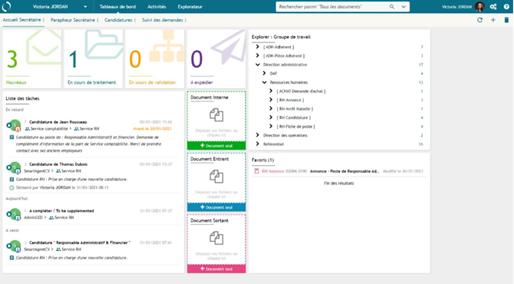
\includegraphics{elise.png}}
\caption{Capture d'écran de Elise}
\label{fig:captureElise}
\end{figure}


L'espace de travail Elise est un regroupement de services et d'utilisateurs. Les espaces de travail permettent de rassembler les documents pour lesquels les utilisateurs et services de l'espace de travail ont une tâche à effectuer.

Il existe trois types d'espaces de travail sous Elise :

\begin{itemize}

\item \textbf{Espace de travail par défaut} : Cet espace de travail est composé du service principal d'utilisateur et de lui-même.
\item \textbf{Espaces de travail personnels} : Espaces de travail que l'utilisateur peut créer et configurer lui-même selon ses besoins.
\item \textbf{Espaces de travail de services} : Espaces de travail prédéfinis que l'utilisateur peut ajouter dans leur liste d'espaces de travail pour en faciliter l'accès.
\end{itemize}

Le tableau de bord d'Elise est une partie personnalisable de l'interface qui permet de proposer des vues de l'espace de travail en fonction des besoins. 

Il existe deux types de tableaux de bord sous Elise :

\begin{itemize}
\item \textbf{Tableaux de bord personnels} : que l'utilisateur peut créer, modifier ou supprimer selon ses besoins.
\item \textbf{Tableaux de bords partagés} : prédéfinis et déployés par l'administrateur.
\end{itemize}

Un tableau de bord d'Elise est un ensemble de widgets. Où un widget est un élément de tableau de bord personnalisable afin d'afficher des informations et/ou de créer une interface vers une fonctionnalité de l'application.

Les différents types de widgets sont :

\begin{itemize}

\item \textbf{Widget compteur} : qui définit les nombres des documents selon leurs types existants dans le courrier.
\item \textbf{Widget graphique} : qui représente les statistiques de type de documents.
\item \textbf{Widget liste de documents} : qui définit les documents selon leurs types existants dans le courrier.
\item \textbf{Widget liste des tâches} : qui définit les tâches affectées aux utilisateurs.
\item \textbf{Widget note} : qui définit les notes de l'utilisateur.
\item \textbf{Widget nouveau document} : qui permet à l'utilisateur d'ajouter un document.
\item \textbf{Widget page web}
\item \textbf{Widget vue dynamique}
\item \textbf{Widget raccourci} : qui est un raccourci à un document ou à un site web.

\end{itemize}

Dans Elise, un document correspond à un enregistrement complet. Un document contient les éléments suivants :

\begin{itemize}
\item \textbf{Propriétés du document} : Les propriétés sont des données contenant les informations associées à un document.
\item \textbf{Fichiers} : Fichiers numériques liés au document et qui sont éditables par les utilisateurs.
\item \textbf{Les tâches} : Les tâches sont des actions à effectuer sur des documents.
\item \textbf{Un processus} : est un ensemble de tâches définissant les actions à réaliser sur un document.
\item \textbf{Les liens} : Propriétés de type URL qui sont ajoutées soit par un automate soit manuellement.
\item \textbf{Historique des événements} : Les événements gardent la trace de toutes les actions effectuées sur le document.
\end{itemize}

Les différents états du document sont les suivants :

\begin{itemize}

\item \textbf{Sans affectation} : État des documents qui ont été créés mais pour lesquels l'ensemble des propriétés obligatoires n'est pas renseigné et/ou aucune tâche n'est encore attribuée. (Cas documents numérisés non encore enregistrés)
\item \textbf{Préparé} : État des documents pour lesquels l'ensemble des propriétés obligatoires est renseigné et au moins une tâche est attribuée. Le changement d'état depuis l'état « Préparé » vers l'état « en cours de traitement » se fait en distribuant le document.
\item \textbf{En circulation} : État des documents pour lesquels il y a des tâches actives en cours de traitement et qui n'ont pas été clôturés. Le changement d'état depuis l'état « En circulation » vers « Clôturé » se fait en clôturant le document.
\item \textbf{Clôturé} : État des documents pour lesquels toutes les tâches qui devaient être effectuées sont terminées et qui ont été clôturés. Le changement d'état depuis l'état « Clôturé » vers l'état « Archivé » se fait en archivant le document.
\item \textbf{Archivé} : État des documents pour lesquels la période d'utilité dans Elise est terminée et qui ne nécessitent donc plus d'être accessibles par les utilisateurs.

\end{itemize}

NeoLedge a une version actuelle du Elise Mobile qui se trouve déjà sur le marché du mobile hébergée dans Play store et App store.

La figure \ref{fig:captureEliseMobile} représente quelques captures d'écran de l'application Elise Mobile existante.\\

% capture d'ecran elimse mobile actuelle
\begin{figure}[!h]
\centering
\fbox{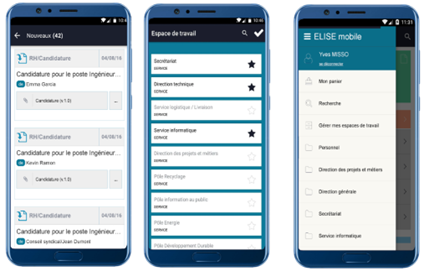
\includegraphics{eliseMobile.png}}
\caption{Capture d'écran de Elise Mobile}
\label{fig:captureEliseMobile}
\end{figure}

Elise Mobile est une application mobile pour plateformes iOS et Android :

\begin{itemize}
\item \textbf{Simple à utiliser} : Elise Mobile est une application intuitive et facile à utiliser. Elle permet de gérer les documents et les tâches depuis n'importe quel endroit et à tout moment.
\item \textbf{Facile à déployer} : Elise Mobile est une application qui ne nécessite pas de configuration particulière. Elle est disponible sur les plateformes iOS et Android.
\item \textbf{Au ROI immédiat} : Elise Mobile permet de gagner du temps et de l'argent en permettant aux utilisateurs de gérer leurs documents et leurs tâches.
\end{itemize}

Elle a été développée en Xamarin depuis le 10 octobre 2018. Elle est en version 1.2.1 jusqu'à présent.

Avec Elise Mobile, les utilisateurs de la solution de Gestion électronique de Contenu Elise peuvent :

\begin{itemize}
%   	Collaborer à distance :
% o	Accéder à l'ensemble de leurs tâches selon leur état de traitement (Nouveaux, En cours, Terminés, etc)
% o	Superviser leurs processus métiers
% o	Effectuer des recherches dans la base documentaire
% 	Décider en quelques instants
% o	Traiter leurs tâches
% o	Valider/Refuser rapidement les actions demandées
% o	Demander/Transférer des tâches
% o	Respecter les délais
% 	Superviser leurs espaces de travail
% o	Accéder aux espaces de travail de leurs différents services
% o	Visualiser les tâches en cours o Contrôler les échéances

\item \textbf{Collaborer à distance} : 
  \begin{itemize}
  \item Accéder à l'ensemble de leurs tâches selon leur état de traitement (Nouveaux, En cours, Terminés, etc)
  \item Superviser leurs processus métiers
  \item Effectuer des recherches dans la base documentaire
  \end{itemize}
\item \textbf{Décider en quelques instants} :
  \begin{itemize}
  \item Traiter leurs tâches
  \item Valider/Refuser rapidement les actions demandées
  \item Demander/Transférer des tâches
  \item Respecter les délais
  \end{itemize}
\item \textbf{Superviser leurs espaces de travail} :
  \begin{itemize}
    \item Accéder aux espaces de travail de leurs différents services
    \item Visualiser les tâches en cours o Contrôler les échéances
  \end{itemize}
\end{itemize}


\subsection{Étude technique}
Elise est une solution d'architecture architecture 3 tiers, illustrée par la figure ci-dessous 
% image architecture_elise
\begin{figure}[H]
  \centering
  \fbox{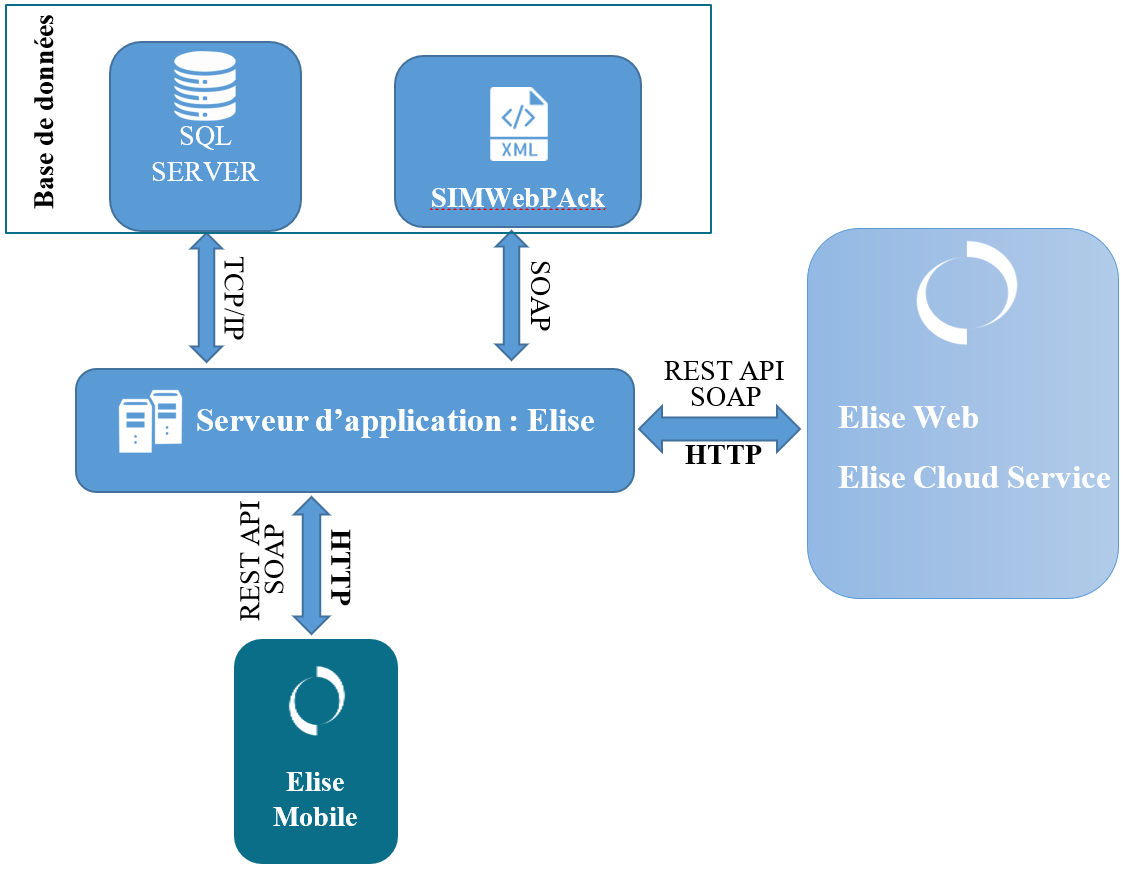
\includegraphics[width=0.8\textwidth]{architecture_elise}}
  \caption{Architecture Elise}
  \label{fig:architecture_elise}
\end{figure}
Cette architecture est composée de trois couches (3 tiers) :

\subsubsection{La couche client (ou la couche présentation)}
C'est la couche frontale de l'application. Elle comprend l'interface utilisateur. Pour notre solution c'est l'application Elise web et les autres applications de ECS : Elise Cloud Service. Et nous allons intégrons notre application mobile à cette couche. Ou toutes les applications de cette couche communiquent avec les autres couches avec des appels web services.

\subsubsection{La couche applicative}
Contient la logique métier fonctionnelle qui pilote les fonctionnalités essentielles d'une application. Dans notre cas, c'est le serveur d'application Elise.

\subsubsection{	La couche d'accès aux données}
Elle contient les données de l'application. Pour notre solution nous avons deux types de base de données ; une base de données relationnelles et une base de données XML.

Cette architecture nous offre la séparation entre l'interface utilisateur, la logique métier et la couche de stockage de données. Cela donne une plus grande flexibilité aux équipes de développement en leur permettant de mettre à jour une partie spécifique d'une application indépendamment des autres parties.


\subsection{Critique de l'existant}
L'étude de l'application existante nous a permis de porter des jugements objectifs afin de projeter de fournir ainsi un système plus fiable.

Parmi les lacunes rencontrées, nous citons :
\begin{itemize}
  % \item Elise est une solution développée de base en ASP. Net Back et front de l'ancienne version d'Asp. Net c'est pour cela l'application actuelle est non responsive et c'est à partir de la version 6 de Elise que NeoLedge a décidé de migrer le front vers les nouvelles technologies. 
  % \item Elise utilise une base de données locale qui est SIMWebPack et qui est une solution proposée par NeoLedge pour enregistrer les documents sous la forme de XML.
  \item La version actuelle d'Elise mobile ne répond pas aux besoins des utilisateurs par rapport à Elise web ce qui invoque de mauvaises expériences utilisateurs.
  \item La version actuelle d'Elise mobile ne renferme pas toutes les fonctionnalités du Elise version web.
\end{itemize}

\subsection{Solution proposée}
Notre solution consiste à mettre en place une solution responsive de Elise qui offre une grande partie des fonctionnalités de la version web actuelle d'Elise tout en gardant les mêmes interfaces pour améliorer l'expérience d'utilisateur. Parmi les fonctionnalités que nous allons traiter, nous citons :

\begin{itemize}
  \item Connecter un utilisateur de Elise à son profil
  \item Consulter les espaces de travail
  \item Accéder à un document
  \item Rechercher un document / un service ou un utilisateur spécifique
  \item Gérer les signatures
  \item Gérer l'abscence
  \item Gérer les documents
  \begin{itemize}
    \item Gérer les tâches d'un document
    \item Possibilité de signer des documents.
    \item Signature possible en utilisant des signatures antérieures ou manuellement.
    \item Possibilité d'utiliser des signatures électroniques.
    \item	Ajouter des fichiers aux documents
  \end{itemize}
  \item Notifications push : Possibilité de recevoir des notifications push pour les mises à jour de documents ou les tâches à effectuer.
\end{itemize}

\section{Méthodologies adoptées}
Au cours de cette section, nous détaillons les méthodologies utilisées qui nous ont permis d'avancer dans la réalisation de notre projet.

\subsection{Méthodologie de modélisation et de conception}
Pour la réalisation d'un projet informatique, une méthode de modélisation et de conception est un procédé qui a pour objectif de permettre de formaliser les étapes préliminaires du développement d'un système afin de rendre ce développement plus fidèle aux besoins du client. C'est pour cela qu'on a choisi UML (Unified Modeling Language) pour la conception de notre projet.\\

\medskip

UML\cite{umlCite} est un langage de modélisation graphique à base de pictogrammes conçu comme une méthode normalisée de visualisation dans les domaines du développement logiciel et en conception orientée objet.



\subsection{Méthodologie de gestion de projet}
Avec les progrès en technologie de l'information et les investissements dans les infrastructures, beaucoup de méthodes de gestion de projet ont vu le jour. Certes, ces méthodes jouent un rôle primordial dans la réussite ou l'échec d'un projet, d'où le choix, représente une décision importante pour les entreprises. Dans cette partie, nous allons expliquer notre choix de la méthode. Il existe en fait deux grandes familles de méthodes de la gestion du projet : les méthodes dites classiques et les méthodes agiles. Nous privilégierons plutôt les méthodes classiques lorsqu'on a une idée précise du projet, avec un planning bien détaillé et où nous avons anticipé tous les risques possibles. Quant aux méthodes Agiles, nous les choisirons plutôt pour les gros projets, celles-ci permettent une meilleure adaptabilité, visibilité et gestion des risques. Nous privilégierons également les méthodes Agiles pour les projets où il n'y a pas de documents détaillés, ou quand le client est indécis. Le client pourra alors voir l'évolution du projet et l'adapter à ses besoins sans pour autant nous obliger à recommencer tout le travail que nous avons fourni depuis le début. Elles sont menées dans un esprit collaboratif et elles s'adaptent aux approches incrémentales. Elles engendrent des produits de haute qualité tout en tenant compte de l'évolution des besoins du client.

\subsubsection{Choix méthodologique}
Notre choix méthodologique et en convenance à notre projet, nous avons opté pour l'utilisation du framework Scrum. C'est en fait le framework le plus utilisé, le plus éprouvé, documenté et supporté. Il s'agit d'un cadre de travail en équipe pluridisciplinaire permettant de répondre à des problèmes complexes et changeants, centré sur l'architecture.
\subsubsection{Pourquoi Scrum}
Dans le cadre de notre projet et afin d'assurer le bon déroulement des différentes phases de ce dernier, nous avons opté pour le framework agile Scrum pour la conception et le développement de notre système pour des raisons bien déterminées. En effet, le framework Scrum s'adapte parfaitement à la décomposition de notre projet de fin d'études.

Il se base sur les avantages suivants :

\begin{itemize}
  \item Plus de souplesse et de réactivité.
  \item Grande capacité d'adaptation au changement grâce à des itérations courtes.
  \item Satisfaire au mieux les besoins du client.
\end{itemize}



SCRUM est une méthodologie agile qui consiste à avoir une équipe soudée orientant le projet au fil de son avancement afin d'atteindre un but. Cette approche est à la fois dynamique et productive, engendre la réalisation des fonctionnalités par itération en incluant la participation du client. Chaque itération peut durer de deux à quatre semaines, à la fin de chaque sprint un produit fonctionnel doit être livré. En effet, Scrum définit trois rôles qui sont :

\begin{itemize}
  \item \textbf{Product Owner }(Le gestionnaire de produit):
  Le responsable du produit de l'équipe projet client et il représente les utilisateurs finaux. C'est lui qui va définir et prioriser la liste des fonctionnalités du produit et choisir la date et le contenu de chaque sprint sur la base des valeurs (charges) qui lui sont communiquées par l'équipe.
  \item \textbf{Scrum Master} (Le maître de Scrum):
  Véritable facilitateur sur le projet, il veille à ce que chacun puisse travailler au maximum de ses capacités en éliminant les obstacles et en protégeant l'équipe des perturbations extérieures.
  \item \textbf{L'équipe de développement} (L'équipe de projet):
  L'équipe de réalisation contient au minimum deux développeurs. Elle regroupe tous les rôles habituellement nécessaires à un projet, à savoir l'architecte, le concepteur, le développeur, le testeur, etc.
\end{itemize}

Le cycle de vie Scrum est illustré par la figure \ref{fig:cycle_de_vie_scrum}.

\begin{figure}[!h]
  \centering
  \fbox{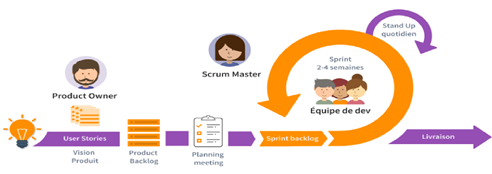
\includegraphics{cycle_de_vie_scrum.png}}
  \caption{Cycle de vie Scrum}
  \label{fig:cycle_de_vie_scrum}
\end{figure}

\section{Environnement de développement}
Avant d'entamer la mise en œuvre de notre projet, nous allons d'abord décrire l'environnement et les outils de travail que nous utiliserons. Nous commencerons par définir l'environnement matériel, suivi de l'environnement logiciel. Enfin, nous présenterons les différents langages et frameworks que nous utiliserons dans le cadre de ce projet.

\subsection{Environnement matériel}

\begin{longtable}{|p{0.3\linewidth}|p{0.6\linewidth}|}
      \hline
      Environnement matériel & Description \\
      \hline
      
      \begin{minipage}{\linewidth}
       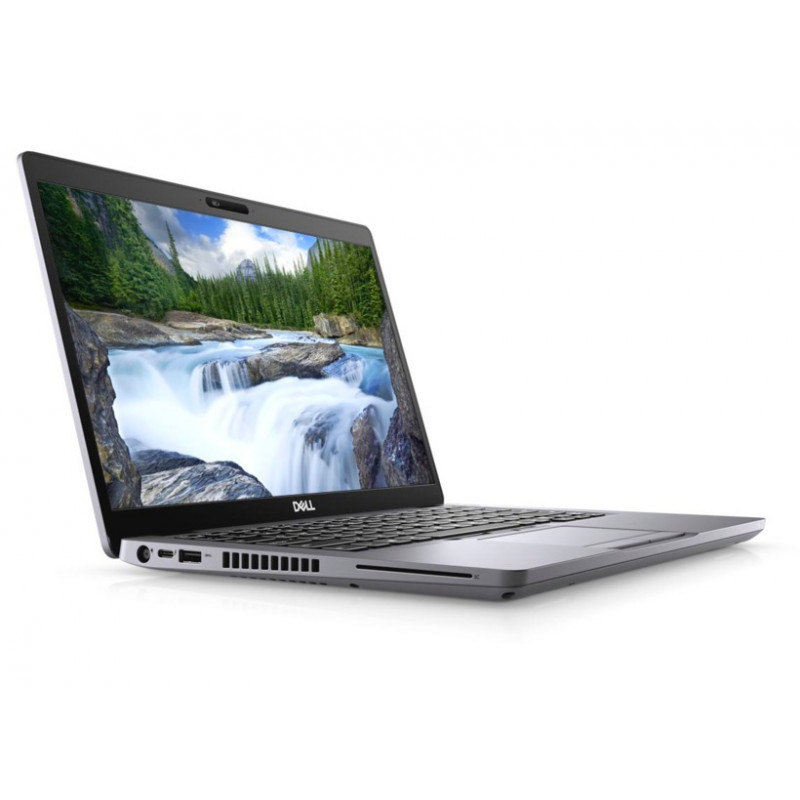
\includegraphics[width=\linewidth]{pc.jpg}
      \end{minipage} &
      \begin{minipage}{\linewidth}
        \vspace{0.2cm}
        \textbf{PC DELL Latitude 5510}
        \begin{itemize}
          \item \textbf{Quantité} : 2
          \item \textbf{Processeur} : Intel Core i7-10610U 
          \item \textbf{Mémoire} : 16 Go DDR4 
          \item \textbf{Stockage} : 512Go SSD 
          \item \textbf{Carte graphique} : NVIDIA GeForce MX250 
          \item \textbf{Système d'exploitation} : Windows 10 
        \end{itemize}
        \vspace{0.2cm}
      \end{minipage} \\
      \hline
      \begin{minipage}{\linewidth}
       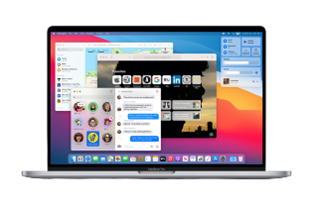
\includegraphics[width=\linewidth]{macbookpro}
      \end{minipage} &
      \begin{minipage}{\linewidth}
        \vspace{0.2cm}
        \textbf{MacBook Pro}
        \begin{itemize}
          \item \textbf{Processeur} : Puce Apple M1 - CPU 8 
          \item \textbf{Mémoire} : 8 Go DDR4
          \item \textbf{Stockage} : 256 Go SSD
          \item \textbf{Système d'exploitation} : macOS Big Sur 
        \end{itemize}
        \vspace{0.2cm}
      \end{minipage} \\


      \hline
      \begin{minipage}{\linewidth}
       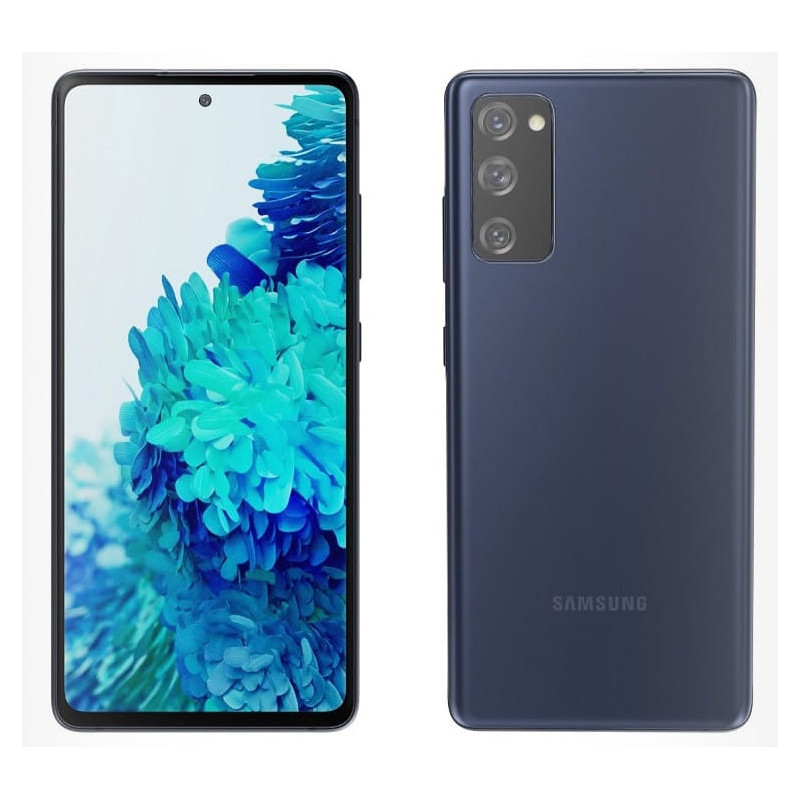
\includegraphics[width=\linewidth]{samsungs20}
      \end{minipage} &
      \begin{minipage}{\linewidth}
        \vspace{0.2cm}
        \textbf{Samsung Galaxy S20 FE 5G}
        \begin{itemize}
          \item \textbf{Processeur} : Cortex-A55 
          \item \textbf{Mémoire} : 12 Go 
          \item \textbf{Stockage} : 128 Go
          \item \textbf{Système d'exploitation} : Android 13
        \end{itemize}
        \vspace{0.2cm}
      \end{minipage} \\

      \hline
      \begin{minipage}{\linewidth}
       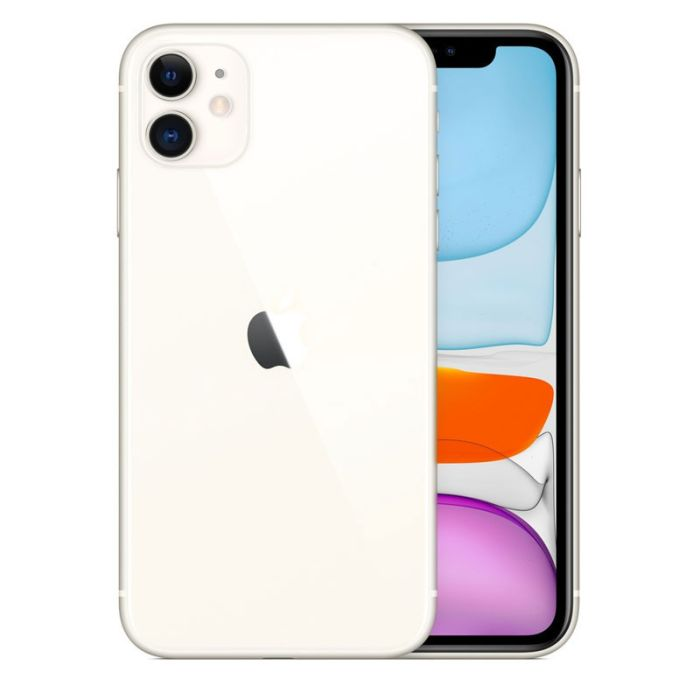
\includegraphics[width=\linewidth]{iphone11}
      \end{minipage} &
      \begin{minipage}{\linewidth}
        \vspace{0.2cm}
        \textbf{Iphone 11}
        \begin{itemize}
          \item \textbf{Processeur} : Apple A13 Bionic
          \item \textbf{Mémoire} : 4 Go
          \item \textbf{Stockage} : 64 Go
          \item \textbf{Système d'exploitation} : iOS 16.3
        \end{itemize}
        \vspace{0.2cm}
      \end{minipage} \\

      \hline
      
      


  \caption{Environnement matériel}
  \label{tab:environnement_materiel}
\end{longtable}

\subsection{Environnement logiciel}
Au cours de cette section, nous dresserons une liste des outils utilisés pour étudier et mettre en place notre application tout au long du projet.

\begin{itemize}
  \item \textbf{Windows 10} :\\
  \begin{minipage}{\linewidth}
    \begin{wrapfigure}{l}{0.125\textwidth}
      \vspace{-0.5cm}
      
\includegraphics[width=1\linewidth]{win10.jpg} 
    \end{wrapfigure}
    Windows 10 est un système d'exploitation de la famille Windows NT développé par la société américaine Microsoft.\cite{windows10}
    \end{minipage}

    \vspace{0.5cm}

  \item \textbf{Visual Studio Code} :\\
  \begin{minipage}{\linewidth}
    \begin{wrapfigure}{l}{0.125\textwidth}
      \vspace{-0.5cm}
      
\includegraphics[width=0.9\linewidth]{vscode.png} 
    \end{wrapfigure}
    Un éditeur de code extensible développé par Microsoft pour Windows, Linux et macOS. Les fonctionnalités incluent
     la prise en charge du débogage, la mise en évidence de la syntaxe, la complétion intelligente du code, les snippets, la refactorisation du code et Git intégrer. \cite{vscode}
  \end{minipage}
    
  \item \textbf{XCode} :\\
  \begin{minipage}{\linewidth}
    \begin{wrapfigure}{l}{0.125\textwidth}
      \vspace{-0.5cm}
      
\includegraphics[width=0.9\linewidth]{xcode} 
    \end{wrapfigure}
    Xcode est un environnement de développement pour macOS, ainsi que pour iOS, watchOS et tvOS. \cite{xcode}
    \end{minipage}

    \vspace{0.5cm}
    \item \textbf{Android Studio} :\\
    \begin{minipage}{\linewidth}
      \begin{wrapfigure}{l}{0.125\textwidth}
        \vspace{-0.5cm}
        
\includegraphics[width=0.9\linewidth]{android.png} 
      \end{wrapfigure}
      Android Studio est un environnement de développement intégré (IDE) pour le développement d'applications Android. Il est basé sur IntelliJ IDEA et est développé par Google. \cite{androidStudio}
    \end{minipage}

    \vspace{0.5cm}

    \item \textbf{Postman} :\\
    \begin{minipage}{\linewidth}
      \begin{wrapfigure}{l}{0.125\textwidth}
        \vspace{-0.5cm}
        
\includegraphics[width=0.9\linewidth]{postman.jpg} 
      \end{wrapfigure}
      Postman est un outil de développement de logiciels qui permet de tester et de déboguer des API. Il permet de créer des requêtes HTTP et de les envoyer à un serveur. Il permet également de créer des collections de requêtes et de les organiser en dossiers. \cite{postman}
    \end{minipage}

    \vspace{0.5cm}
    \item \textbf{Git} :\\
    \begin{minipage}{\linewidth}
      \begin{wrapfigure}{l}{0.125\textwidth}
        \vspace{-0.5cm}
        
\includegraphics[width=0.9\linewidth]{git.jpg} 
      \end{wrapfigure}
      Git est un logiciel de gestion de versions décentralisé. Il permet de gérer les versions d'un projet informatique et de collaborer avec d'autres développeurs. \cite{git}
    \end{minipage}
    

    \vspace{0.5cm}
    \item \textbf{Azure DevOps} :\\
    \begin{minipage}{\linewidth}
      \begin{wrapfigure}{l}{0.125\textwidth}
        \vspace{-0.5cm}
        
\includegraphics[width=0.9\linewidth]{AzureDevOps.png} 
      \end{wrapfigure}
      Azure DevOps est un ensemble d'outils de développement logiciel en tant que service (SaaS) fourni par Microsoft. Il fournit des services de gestion de projets, de gestion de code source, de gestion de tests et de gestion de la qualité du logiciel. \cite{azureDevOps}
    \end{minipage}

    \vspace{0.5cm}
    \item \textbf{Figma} :\\
    \begin{minipage}{\linewidth}
      \begin{wrapfigure}{l}{0.125\textwidth}
        \vspace{-0.8cm}
        
\includegraphics[width=0.9\linewidth]{figma.jpg} 
      \end{wrapfigure}
      Figma est un outil de conception graphique. Il permet de créer des maquettes de sites web et d'applications mobiles. \cite{figma}
    \end{minipage}

    \vspace{0.5cm}
    \item \textbf{Draw.io} :\\
    \begin{minipage}{\linewidth}
      \begin{wrapfigure}{l}{0.125\textwidth}
        \vspace{-0.5cm}
        
\includegraphics[width=0.9\linewidth]{drawio.png} 
      \end{wrapfigure}
      Draw.io est un logiciel de dessin graphique multiplateforme gratuit et open source développé en HTML5 et JavaScript. Son interface peut être utilisée pour créer tous types de diagrammes. \cite{drawio}
    \end{minipage}

    \vspace{0.5cm}
    \item \textbf{Microsoft Teams} :\\
    \begin{minipage}{\linewidth}
      \begin{wrapfigure}{l}{0.125\textwidth}
        \vspace{-0.5cm}
        
\includegraphics[width=0.9\linewidth]{teams.png} 
      \end{wrapfigure}
      Microsoft Teams est un logiciel de messagerie instantanée et de collaboration en ligne développé par Microsoft. Il permet de créer des salons de discussion, de partager des fichiers et de collaborer en temps réel. \cite{teams}
    \end{minipage}

    \vspace{0.5cm}
    \item \textbf{Latex} :\\
    \begin{minipage}{\linewidth}
      \begin{wrapfigure}{l}{0.125\textwidth}
        \vspace{-0.5cm}
        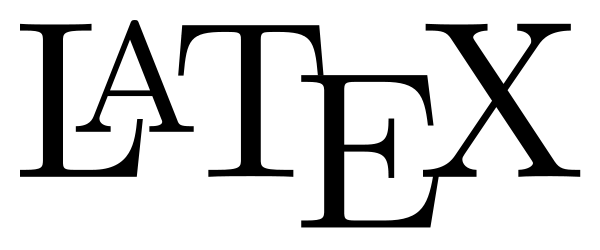
\includegraphics[width=0.9\linewidth]{latex.png} 
      \end{wrapfigure}
      LaTeX est un langage de description de documents. Il permet de créer tous types de documents. Il est utilisé pour la rédaction de livres, de rapports, de thèses, de journaux, de présentations, de documents techniques, etc. \cite{latex}
    \end{minipage}

    \vspace{0.5cm}
    \item \textbf{NodeJs} :\\
    \begin{minipage}{\linewidth}
      \begin{wrapfigure}{l}{0.125\textwidth}
        \vspace{-0.5cm}
        
\includegraphics[width=0.9\linewidth]{nodejs.png}
      \end{wrapfigure}
      Node.js est une plateforme logicielle libre en JavaScript, orientée vers les applications réseau évènementielles hautement concurrentes. \cite{nodejs}
    \end{minipage}
    \vspace{0.5cm}

    \item \textbf{Firebase} :\\
    \begin{minipage}{\linewidth}
      \begin{wrapfigure}{l}{0.125\textwidth}
        \vspace{-0.5cm}
        
\includegraphics[width=0.9\linewidth]{firebase} 
      \end{wrapfigure}
      Firebase est un ensemble de services d'hébergement pour n'importe quel type d'application.
      Il propose d'héberger en NoSQL et en temps réel des bases de données, du contenu, et des notifications, etc. \cite{firebase}
    \end{minipage}
  \vspace{0.5cm}

    \item \textbf{json-server} :\\
    \begin{minipage}{\linewidth}
      \begin{wrapfigure}{l}{0.125\textwidth}
        \vspace{-0.5cm}
        
\includegraphics[width=0.9\linewidth]{json-server} 
      \end{wrapfigure}
      json-server est un outil qui permet de créer un serveur REST à partir d'un fichier JSON ou d'un fichier JavaScript. \cite{jsonServer}
    \end{minipage}
  \end{itemize}


  \subsection{Technologies utilisées}

  \begin{itemize}
    \item \textbf{Ionic} :\\
    \begin{minipage}{\linewidth}
      \begin{wrapfigure}{l}{0.125\textwidth}
        \vspace{-0.5cm}
        
\includegraphics[width=0.9\linewidth]{ionic.png} 
      \end{wrapfigure}
      Ionic est un UI toolkit open source pour la création d'applications mobiles performantes et de haute qualité à l'aide de technologies web telles que HTML, CSS et JavaScript, avec des intégrations pour des frameworks populaires tels que Angular, React et Vue. \cite{ionic}
    \end{minipage}
  
    \vspace{0.5cm}
  
    \item \textbf{Vue3} :\\
    \begin{minipage}{\linewidth}
      \begin{wrapfigure}{l}{0.125\textwidth}
        \vspace{-0.5cm}
        
\includegraphics[width=0.9\linewidth]{vue.png} 
      \end{wrapfigure}
      Vue.js est un framework JavaScript open source pour la création d'interfaces utilisateur et d'applications web monopages. \cite{vuejs}
    \end{minipage}
  
    \vspace{0.5cm}
  
    \item \textbf{Capacitor} :\\
    \begin{minipage}{\linewidth}
      \begin{wrapfigure}{l}{0.125\textwidth}
        \vspace{-0.5cm}
        
\includegraphics[width=0.9\linewidth]{capacitor.png} 
      \end{wrapfigure}
      Capacitor est un runtime natif open source pour la création d'applications Web natives. Il permet de créer des applications iOS, Android et des applications Web progressives multiplateformes à l'aide de JavaScript, HTML et CSS. \cite{capacitor}
    \end{minipage}
  
    \vspace{0.5cm}
  
    \item \textbf{Typescript} :\\
    \begin{minipage}{\linewidth}
      \begin{wrapfigure}{l}{0.125\textwidth}
        \vspace{-0.5cm}
        
\includegraphics[width=0.9\linewidth]{typescript.png} 
      \end{wrapfigure}
      TypeScript est un langage de programmation libre et open source développé par Microsoft. Il est un sur-ensemble de JavaScript, c'est-à-dire qu'il ajoute des fonctionnalités à ce dernier. \cite{typescript}
    \end{minipage}
  
    \vspace{0.5cm}
  
    \item \textbf{Javascript} :\\
    \begin{minipage}{\linewidth}
      \begin{wrapfigure}{l}{0.125\textwidth}
        \vspace{-0.5cm}
        
\includegraphics[width=0.9\linewidth]{javascript.png} 
      \end{wrapfigure}
      JavaScript est un langage de programmation de scripts principalement employé dans les pages web interactives et à ce titre est une partie essentielle des applications web. \cite{javascript}
    \end{minipage}

    \vspace{0.5cm}
  
    \item \textbf{Pinia} :\\
    \begin{minipage}{\linewidth}
      \begin{wrapfigure}{l}{0.125\textwidth}
        \vspace{-0.5cm}
        
\includegraphics[width=0.9\linewidth]{pinia.png} 
      \end{wrapfigure}
      Pinia est une bibliothèque de magasin et un framework de gestion d'état pour Vue.js. Conçu principalement pour créer des applications Web frontales, il utilise une syntaxe déclarative et propose sa propre API de gestion d'état. \cite{pinia}
    \end{minipage}
    
    \vspace{0.5cm}
  
    \item \textbf{PlantUML} :\\
    \begin{minipage}{\linewidth}
      \begin{wrapfigure}{l}{0.125\textwidth}
        \vspace{-0.5cm}
        
\includegraphics[width=0.9\linewidth]{plantuml.png} 
      \end{wrapfigure}
      PlantUML est un outil open-source permettant aux utilisateurs de créer des diagrammes à partir d'un langage de texte simple. \cite{plantuml}
    \end{minipage}

    \item \textbf{Jest} :\\
    \begin{minipage}{\linewidth}
      \begin{wrapfigure}{l}{0.125\textwidth}
        \vspace{-0.5cm}
        
\includegraphics[width=0.9\linewidth]{jest.png} 
      \end{wrapfigure}
      Jest est un framework de test JavaScript construit sur Jasmine et maintenu par Meta. Il a été conçu et construit en mettant l'accent sur la simplicité et la prise en charge des grandes applications Web. \cite{jest}
    \end{minipage}
  
    \vspace{0.5cm}
    \item \textbf{Express} :\\
    \begin{minipage}{\linewidth}
      \begin{wrapfigure}{l}{0.125\textwidth}
        \vspace{-0.5cm}
        
\includegraphics[width=0.9\linewidth]{express.png}
      \end{wrapfigure}
      Express est un framework pour construire des applications web basées sur Node.js. C'est de fait le framework standard pour le développement de serveur en Node.js.  \cite{express}
    \end{minipage}

  
  \end{itemize}



\section*{Conclusion}
Au cours de ce chapitre qui constitue une étape primordiale pour fixer les repères de notre projet. Nous avons présenté l'organisme d'accueil et les attentes du projet. En effet, nous avons mené une étude de l'existant afin de mieux cerner les fonctionnalités de notre solution révélant les limites de la solution existante. Nous avons également déterminé le cadre du travail ainsi que la méthodologie à emprunter lors de ce projet.

Dans le chapitre qui suit nous allons décrire la conception de l'application en détaillant ses spécifications, ses acteurs et le product backlog contenant les fonctionnalités de l'application.


\chapter{Planification du Backlog Product}
\addcontentsline{toc}{chapter}{Planification du Backlog Product}
\markboth{Planification du Backlog Product}{Planification du Backlog Product}

\label{chap:analyseEtConception}
% section starts from 1 
%\minitoc

\section*{Introduction}
Afin de pouvoir implémentées les fonctionnalités recensées au début de ce projet, nous
s'intéressons dans ce chapitre à l'étude conceptuelle de notre application. C'est une phase de spécification et de modélisation conceptuelle basée sur le langage UML à travers les diagrammes de cas d'utilisation, les diagrammes de séquences et classes. Ceci nous permet de tracer une meilleure stratégie d'implémentation des besoins fonctionnels tout en respectant les contraintes identifiées. Ensuite, nous exposerons les besoins non fonctionnels ainsi que notre backlog de produit.

\section{Identifications des acteurs}
Un utilisateur est une entité extérieure au système de modélisation qui représente et
interagit directement avec une personne, un appareil. Chaque acteur dispose d'un ensemble
d'actions correspondant à la fonction dont il a besoin. Dans notre projet

L'application « Elise » Mobile fait intervenir plusierus acteurs comme le montre le tableau ci-après.

\begin{table}[h]
\setlength\tabcolsep{3pt}
\centering
\begin{tabularx}{\textwidth}{|c|L|}
\hline
Acteur  &  Rôles \\ 
\hline
\textbf{Collaborateur}  &  Accéde aux documents qui lui sont partagés, peut les modifier et les partager selon les tâches qui lui sont assignées \\ \hline
\textbf{Secrétaire}  &  Même rôle que le collaborateur avec en plus l'accès aux documents partagés par les autres de son service et les documents partagés par les autres services des collaborateurs \\ \hline
\textbf{Chef de service}  &  Même rôle que le secrétaire avec en plus l'accès aux documents partagés par les autres services subalternes \\ \hline
\end{tabularx}
\caption{Acteurs de l'application}
\label{tab:acteurs}
\end{table}



% note
\begin{small}
  Ces rôles/droits sont définis et appliqués par défaut par le système. Il est possible de les modifier selon les besoins spécifiques du client.
\end{small}


\section{Besoins fonctionnels des collaborateurs}
Notre application est desinée aux utilisateurs suivants : les collaborateurs, les secrétaires et les chefs de service. Chacun d'eux dispose d'un ensemble d'actions correspondant à la fonction dont il a besoin.

\begin{itemize}
% \item \textbf{Authentification} : L'utilisateur doit pouvoir s'authentifier à l'application pour pouvoir accéder à ses documents.
% \item \textbf{Consultation de profil} : L'utilisateur doit pouvoir consulter son profil.
% \item \textbf{Modification de profil} : L'utilisateur doit pouvoir modifier son profil.
% \item \textbf{Declaration d'absence} : L'utilisateur doit pouvoir déclarer son absence.
% \item \textbf{Annulation d'absence} : L'utilisateur doit pouvoir annuler son absence.
% \item \textbf{Affectation de delegé} : L'utilisateur doit pouvoir affecter un ou plusieurs délégué(s) pour le remplacer en cas d'absence.
% \item \textbf{Suppression de delegé} : L'utilisateur doit pouvoir supprimer un ou plusieurs délégué(s) affecté(s).
% \item \textbf{Recherche d'un utilisateur/service} : L'utilisateur doit pouvoir rechercher un utilisateur ou un service.
% \item \textbf{Reception de notification} : L'utilisateur doit pouvoir recevoir une notification de rappel.
% \item \textbf{Désactivation de notification} : L'utilisateur doit pouvoir désactiver les notifications.
% \item \textbf{Consulter espace de travail utilisateur} : L'utilisateur doit pouvoir consulter son espace de travail.
% \item \textbf{Consulter espace de travail personnalisé} : L'utilisateur doit pouvoir consulter son espace de travail personnalisé.
% \item \textbf{Supprimer espace de travail personnalisé} : L'utilisateur doit pouvoir supprimer son espace de travail personnalisé.
% \item \textbf{Modifier espace de travail personnalisé} : L'utilisateur doit pouvoir modifier son espace de travail personnalisé.
% \item \textbf{Ajouter un espace de travail personnalisé} : L'utilisateur doit pouvoir ajouter un espace de travail personnalisé.
% \item \textbf{Accéder aux espaces de travail de ses différents services} : L'utilisateur doit pouvoir accéder aux espaces de travail de ses différents services.
% \item \textbf{Consulter tableau de bord partagé et personnel} : L'utilisateur doit pouvoir consulter son tableau de bord partagé et personnel.
% \item \textbf{Consulter les widgets du tableau de bord personnel} : L'utilisateur doit pouvoir consulter les widgets de son tableau de bord personnel.
% \item \textbf{Ajouter un widget dans le tableau de bord personnel} : L'utilisateur doit pouvoir ajouter un widget dans son tableau de bord personnel.
% \item \textbf{Supprimer un widget dans le tableau de bord personnel} : L'utilisateur doit pouvoir supprimer un widget dans son tableau de bord personnel.
% \item \textbf{Configurer un widget du tableau de bord personnel} : L'utilisateur doit pouvoir configurer un widget de son tableau de bord personnel.
% \item \textbf{Ajouter un tableau de bord personnel} : L'utilisateur doit pouvoir ajouter un tableau de bord personnel.
% \item \textbf{Supprimer un tableau de bord personnel} : L'utilisateur doit pouvoir supprimer un tableau de bord personnel.
% \item \textbf{Modifier un tableau de bord personnel} : L'utilisateur doit pouvoir modifier un tableau de bord personnel.
% \item \textbf{Rechercher un document selon le filtre} : L'utilisateur doit pouvoir rechercher un document selon le filtre.
% \item \textbf{Accéder à l'ensemble de ses tâches} : L'utilisateur doit pouvoir accéder à l'ensemble de ses tâches.
% \item \textbf{Superviser son processus métier} : L'utilisateur doit pouvoir superviser son processus métier.
% \item \textbf{Démarrer une tâche dans un document} : L'utilisateur doit pouvoir démarrer une tâche dans un document.
% \item \textbf{Modifier informations d'un document} : L'utilisateur doit pouvoir modifier les informations d'un document.
% \item \textbf{Consulter les fichiers d'un document} : L'utilisateur doit pouvoir consulter les fichiers d'un document.
% \item \textbf{Supprimer un fichier d'un document} : L'utilisateur doit pouvoir supprimer un fichier d'un document.
% \item \textbf{Ajouter un fichier à un document} : L'utilisateur doit pouvoir ajouter un fichier à un document.
% \item \textbf{Consulter l'historique d'un document} : L'utilisateur doit pouvoir consulter l'historique d'un document.
% \item \textbf{Consulter les tâches d'un document} : L'utilisateur doit pouvoir consulter les tâches d'un document.
% \item \textbf{Supprimer une tâche d'un document} : L'utilisateur doit pouvoir supprimer une tâche d'un document.
% \item \textbf{Ajouter une tâche à un document} : L'utilisateur doit pouvoir ajouter une tâche à un document.
% \item \textbf{Consulter l'historique d'une tâche} : L'utilisateur doit pouvoir consulter l'historique d'une tâche.
% \item \textbf{Consulter les signatures} : L'utilisateur doit pouvoir consulter les signatures.
% \item \textbf{Ajouter une signature} : L'utilisateur doit pouvoir ajouter une signature.
% \item \textbf{Supprimer une signature} : L'utilisateur doit pouvoir supprimer une signature.
% \item \textbf{Signer un document manuellement} : L'utilisateur doit pouvoir signer un document manuellement.
% \item \textbf{Signer un document à l'aide des signatures enregistrées} : L'utilisateur doit pouvoir signer un document à l'aide des signatures enregistrées.

\item \textbf{Authentification}
% \item \textbf{Consultation de profil}
% \item \textbf{Modification de profil}
\item \textbf{Gérer le profil}
% \item \textbf{Declaration d'absence}
% \item \textbf{Annulation d'absence}
% \item \textbf{Affectation de delegé}
% \item \textbf{Suppression de delegé}
% \item \textbf{Recherche d'un utilisateur/service}
\item \textbf{Gérer l'absence}
% \item \textbf{Reception de notification}
% \item \textbf{Désactivation de notification}
\item \textbf{Gérer les notifications}
% \item \textbf{Consulter espace de travail utilisateur}
% \item \textbf{Consulter espace de travail personnalisé}
% \item \textbf{Supprimer espace de travail personnalisé}
% \item \textbf{Modifier espace de travail personnalisé}
% \item \textbf{Ajouter un espace de travail personnalisé}
\item \textbf{Accéder aux espaces de travail de ses différents services}
% \item \textbf{Consulter tableau de bord partagé et personnel}
% \item \textbf{Consulter les widgets du tableau de bord personnel}
% \item \textbf{Ajouter un widget dans le tableau de bord personnel}
% \item \textbf{Supprimer un widget dans le tableau de bord personnel}
% \item \textbf{Configurer un widget du tableau de bord personnel}
% \item \textbf{Ajouter un tableau de bord personnel}
% \item \textbf{Supprimer un tableau de bord personnel}
% \item \textbf{Modifier un tableau de bord personnel}
\item \textbf{Rechercher des documents}
\item \textbf{Consulter les documents favoris}
\item \textbf{Accéder à l'ensemble de ses tâches}
% \item \textbf{Superviser son processus métier}
% \item \textbf{Démarrer une tâche dans un document}
% \item \textbf{Modifier informations d'un document}
% \item \textbf{Consulter les fichiers d'un document}
% \item \textbf{Supprimer un fichier d'un document}
% \item \textbf{Ajouter un fichier à un document}
\item \textbf{Gérer les fichiers d'un document}
\item \textbf{Consulter l'historique d'un document}
% \item \textbf{Consulter les tâches d'un document}
% \item \textbf{Supprimer une tâche d'un document}
% \item \textbf{Ajouter une tâche à un document}
% \item \textbf{Consulter l'historique d'une tâche}
\item \textbf{Gérer les tâches d'un document}
% \item \textbf{Consulter les signatures}
% \item \textbf{Ajouter une signature}
% \item \textbf{Supprimer une signature}
\item \textbf{Gérer les signatures}
% \item \textbf{Signer un document manuellement}
% \item \textbf{Signer un document à l'aide des signatures enregistrées}
\item \textbf{Signer un document}

\end{itemize}



% \section{Conception}
% \subsection{Diagramme de cas d'utilisation}
% % \begin{figure}[h]
% % \centering
% % \includegraphics[width=0.8\textwidth]{cas}
% % \caption{Diagramme de cas d'utilisation}
% % \end{figure}
% % include pdf
% Pour répondre aux besoins fonctionnels décrits ci-dessus, nous allons présenter le diagramme de cas d'utilisation global illustré dans la figure ci-dessous.
% \begin{figure}[!h]
% \centering
% 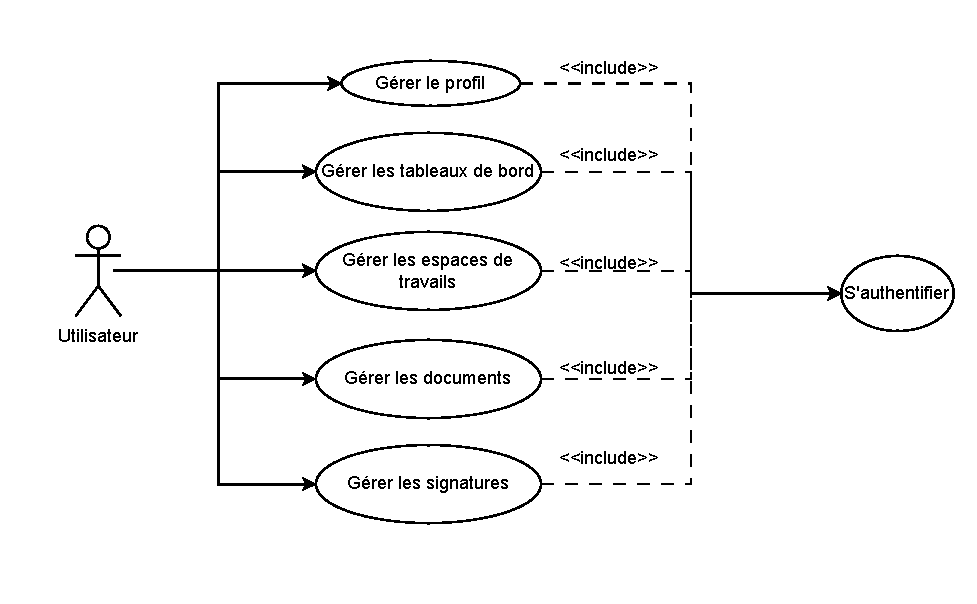
\includegraphics[width=0.6\textwidth]{useCaseGeneral}
% \caption{Diagramme de cas d'utilisation global}
% \end{figure}

% \section{Le pilotage du projet par SCRUM}
% Scrum est basé sur un ensemble de concepts permettant d'assurer une bonne gestion des projets : rôle, artefacts, sprint et réunion.

% \subsection{Identification de l'équipe SCRUM}
% L'équipe joue un rôle capital dans Scrum : elle permet d'optimiser la productivité et la
% flexibilité.

% Afin de parvenir à ces objectifs, elle doit s'auto organiser et être multi compétente. Elle doit également avoir un champ d'action suffisant pour la soutenir dans la réalisation de son travail
% Dans le contexte de notre projet, on trouve :

% \begin{itemize}
%   \item \textbf{Product Owner} Quentin DEMARTHE
%   \item \textbf{Scrum Master} Rabii MEJAI
%   \item \textbf{Equipe de développement} : Mohamed Youssef CHLENDI, Raed CHARRAD
% \end{itemize}

\section{Les User Stories}
Une user story est une expression qui décrit un point de vue de l'utilisateur et a pour objectif de donner une valeur au travail. Elle contient généralement trois éléments descriptifs de la fonctionnalité : 

  \textbf{Qui est l'utilisateur ? Qu'est-ce qu'il veut faire ? Et pourquoi veut-il le faire ?}

L'expression qui est souvent utilisée pour formuler une user story est « En tant que \textbf{'qui'}, je veux \textbf{'quoi'} afin de \textbf{'pourquoi'} ». Cette structure permet de décrire de manière concise les besoins des utilisateurs et de les prendre en compte dans la planification et le développement du produit.


% Jump page
\newpage
\begin{landscape}



  \begin{adjustwidth}{-1cm}{}
    % \usepackage{longtable}
      
      \begin{longtable}{|c|p{3cm}|p{8cm}|c|c|p{2cm}|p{2cm}|c|}
        % \centering
        \hline
    ID  &   User Story  &  Description   &  Compléxité  &  Priorité  &  Période  &  Sprint  &   \\
    % \hline
    % 1  &  Gestion d'accès et de profil  &  Texte sur une seule ligne  &  Ligne 1  &  1 \\
    \hline
    TS1  &  Formation sur la solution Elise  &  En tant que membre de l'équipe scrum, je souhaite comprendre pleinement la fonctionnalité du système Elise afin de reproduire sa logique dans une application mobile.   &  Moyenne  &  2  &  Du 8  à 12  Février  &  \multirow{3}{2cm}{
      \begin{center}
        
        \textbf{Sprint 1 :} Préparation de l’environnement du travail et étude de la solution
      \end{center}
      }  &  \multirow{19}{2.5cm}[-10.5ex]{\textbf{Release 1}}  \\
    \cline{1-6}
    TS2  &  Formation en développement mobile avec Ionic Vue et Capacitor  &  En tant que scrum team, je souhaite me former au développement mobile en utilisant les technologies Ionic Vue et Capacitor. Cette formation doit me permettre de maîtriser les compétences essentielles pour créer des applications mobiles multiplateformes de qualité.  &  Moyenne  &  1  &  Du 13  à 16 Février  &  &  \\
    \cline{1-6}
    TS3  &  Installer et configurer l'environnement de développement  &  En tant que développeur, je veux installer et configurer le logiciel Visual Studio Code et Android studio pour travailler sur le projet en utilisant les technologies suivantes: Ionic Vue, .NET Core 6 et Capacitor.  &  Facile  &  1  &  16 Février  &  & \\
    \cline{1-6}
    TS4  &  Développer des prototypes  &  En tant que développeur, je veux développer des prototypes de l'application mobile afin de tester les fonctionnalités et de valider les choix techniques.  &  Moyenne  &  1  &  Du 17  à 22 Février  &  & \\

    \cline{1-7}

    US1 & Création de signature & En tant qu'utilisateur, je veux créer une signature numérique en dessinant ma signature à l'aide de mon doigt ou de mon stylet sur l'écran tactile de mon appareil mobile, afin de la réutiliser facilement lors de la signature de documents. & Moyenne & 2 & Du 23 à 27 Février  & \multirow{5}{2cm}{\textbf{Sprint 2 :} 
Gestion des signatures}  & \\

    % afficher la liste des signatures
    \cline{1-6}
    US2 & Affichage de la liste des signatures & En tant qu'utilisateur, je veux afficher la liste des signatures que j'ai créées auparavant, afin de pouvoir les utiliser pour signer un document. & Facile & 1 &  du 27 à 28 Février &  & \\

    \cline{1-6}
    US3 & Suppression de signature & En tant qu'utilisateur, je veux supprimer une signature numérique que j'ai créée auparavant, en cas de besoin ou si ma signature a changé, afin de ne pas utiliser une signature obsolète ou inexacte. & Facile & 2 &   28 Février &  &\\

    \cline{1-6}
    US4 & Visualisation de signature & En tant qu'utilisateur, je veux pouvoir visualiser ma signature numérique, pour m'assurer qu'elle est correcte. & Moyenne & 2 &  du 1 à 2 Mars &  &\\

    \cline{1-6}
    US4 & Ajout de signature à l'aide d'OCR & En tant qu'utilisateur, je veux ajouter ma signature en utilisant la camera de mon appareil ou une image, afin de gagner du temps et de faciliter le processus de signature. & Difficile & 2 & du 3 à 9 Mars &  & \\



    \cline{1-7}
    US11&Recherche de documents&En tant qu'utilisateur, je veux rechercher des documents en utilisant différents critères, tels que le nom, la date, le type ou le contenu, afin de trouver rapidement les documents dont j'ai besoin.&Difficile&2&du 10 à 13 Mars&\multirow{7}{2cm}{\textbf{Sprint 3 :} 
    Gestion des documents}&\\

    \cline{1-6}
    US12&Afficher documents favoris&En tant qu'utilisateur, je veux affiches les favoris, afin de trouver rapidement les documents dont j'ai besoin. &Moyenne&2&du 14 à 15 Mars&&\\

    \cline{1-6}
    US6&Accès aux documents&En tant qu'utilisateur, je veux récupérer les informations relatives à un document, telles que la date de création, les utilisateurs qui ont accédé au document et les tâches associées, afin de suivre l'historique du document et de mieux comprendre son contexte, les modifier ou de les signer.&Moyenne&2&du 16 à 17 Mars&&\\
    \cline{1-6}
    US6&Télécharger un document&En tant qu'utilisateur, je veux télécharger les fichiers attachés à un document, afin de garder une copie locale.&Moyenne&2&du 16 à 17 Mars&&\\

    \cline{1-6}
    
    US7&Consulter les fichiers d'un document&En tant qu'utilisateur, je veux consulter la liste des fichiers attachés à un document, afin de les visualiser. &Moyenne&2&du 18 à 19 Mars&&\\
    
    \cline{1-6}
    US8&Consulter les tâches&En tant qu'utilisateur, je veux consulter la liste des tâches associées à un document, afin de suivre l'état d'avancement des tâches et de savoir qui est responsable de chaque tâche. &Moyenne&2&du 20 à 21 Mars&&\\


    \cline{1-6}
    US9&Ajout de fichiers à un document&En tant qu'utilisateur, je veux ajouter des fichiers supplémentaires à un document existant, afin de rassembler toutes les informations nécessaires dans un seul document et de faciliter le partage des informations.&Moyenne&2&du 21 à 22 Mars&&\\
    \cline{1-6}
    % US10&Suppression d'un fichier dans un document&En tant qu'utilisateur, je veux pouvoir supprimer un fichier spécifique qui a été ajouté à un document, afin de maintenir la pertinence et la validité des documents stockés dans l'application. &Moyenne&2&du 23 à 24 Mars&&\\
    % \cline{1-6}


    %   % Demander une tache
    % US13&Demander une tâche&En tant qu'utilisateur, je veux demander une tâche dans un document en assignant une personne responsable, en définissant une date d'échéance et en ajoutant des commentaires, afin de faciliter la collaboration et le suivi des tâches.&Difficile&2&&&\\	

    \cline{1-6}
    % Transferer une tache a un autre utilisateur
    US14&Transferer une tâche&En tant qu'utilisateur, je veux transferer une tâche dans un document a un autre utilisateur, afin que ce dernier puisse la prendre en charge.&Moyenne&2&&&\\
    \cline{1-6}
    US15&Traitment d'une tâche dans un document&En tant qu'utilisateur, je veux pouvoir terminer une tâche dans un document en la marquant comme terminée et en ajoutant des commentaires sur le travail effectué, afin de clôturer la tâche et de faciliter le suivi du projet. &Moyenne&2&&&\\


    % \cline{1-6}
    % US5 & Vérification d'authenticité de la signature & En tant qu'utilisateur, je veux vérifier l'authenticité d'une signature numérique ajoutée à un document, pour m'assurer que la signature est valide et qu'elle n'a pas été falsifiée ou modifiée depuis sa création. & Difficile & 2 & 3 Avril  &  & \\

    \cline{1-7}

    US16&Visualisation de fichiers&En tant qu'utilisateur, je veux visualiser des fichiers stockés dans le document, afin de consulter leur contenu sans avoir besoin d'une autre application ou d'un autre dispositif.&Difficile&2&du 20 à 26 Mars&\multirow{2}{2cm}{\textbf{Sprint 4 :} Visualisation et signature de fichiers}&\\

    \cline{1-6}
    US17&Téléchargement de fichiers&En tant qu'utilisateur, je veux télécharger un fichier, afin d'avoir une copie locale du fichier sur mon appareil.&Difficile&2&du 27 à 28 Mars&&\\
    \cline{1-6}

    US17&Signature de fichiers avec image&En tant qu'utilisateur, je souhaite signer des fichiers avec image, Je veux être en mesure de sélectionner une signature pré-enregistrée parmi celles que j'ai créées précédemment, en utilisant simplement un système de glisser-déposer pour l'appliquer au document à signer.&Difficile&2&du 27 à 28 Mars&&\\
    \cline{1-6}

    US18&Signature de fichiers a main&En tant qu'utilisateur, je souhaite signer des fichiers a main. Je veux signer le document directement en utilisant une méthode de signature manuscrite, en dessinant ma signature.&Difficile&2&du 29 à 30 Mars&&\\
    
    \cline{1-6}
    % Deplacer signature non enregistrée
    US19&Deplacer les signatures non enregistrées&En tant qu'utilisateur, je souhaite déplacer les signatures non enregistrées, afin de les positionner correctement.&Difficile&2&31 Mars&&\\
    
    \cline{1-6}
    % Supprimer signature non enregistrée
    US19&Supprimer les signatures non enregistrées&En tant qu'utilisateur, je souhaite supprimer les signatures non enregistrées, afin d'annuler la signature.&Difficile&2&31 Mars&&\\

    % Confirmer ou annuler la signature
    \cline{1-6}
    US20&Confirmer ou annuler la signature&En tant qu'utilisateur, je souhaite confirmer ou annuler la signature, afin de la valider ou de la supprimer.&Difficile&2&31 Mars&&\\
    

    \cline{1-8}
    US21&Connexion simple avec le mot de passe et l'email&En tant qu'utilisateur, je veux connecter à l'application Elise Mobile en utilisant mes identifiants (adresse e-mail et mot de passe).&Moyenne&2&du 4 à 5 Avril&\multirow{3}{2cm}{\textbf{Sprint 5 :} Gestion d' authentification simple }&\multirow{11}{2.5cm}{Release 2}\\

    \cline{1-6}
    US22&Déconnexion&En tant qu'utilisateur, je veux déconnecter de l'application Elise Mobile afin de protéger mes informations et données personnelles en cas de perte ou de vol de mon téléphone portable. La déconnexion doit être facile d'accès et rapide.&Moyenne&2&6 Avril&&\\
    \cline{1-6}
    US23&Formation sur le protocole OIDC&En tant que scrum team, je souhaite me former sur le protocole OIDC. Cette formation doit me permettre de maîtriser les compétences essentielles pour mettre en place une authentification et une autorisation sécurisées dans notre application mobile.&&&du 6 à 7 Avril&&\\
    \cline{1-6}
    US24&Connexion à l'aide du protocole OIDC&En tant qu'utilisateur, je veux pouvoir me connecter à l'application Elise Mobile en utilisant mon compte Microsoft.&Difficle&2&du 10 à 17 Avril&&\\

    \cline{1-6}
    US25&Déconnexion&En tant qu'utilisateur, je veux déconnecter de l'application Elise Mobile afin de protéger mes informations et données personnelles en cas de perte ou de vol de mon téléphone portable. La déconnexion doit être facile d'accès et rapide.&Moyenne&2&18 Avril&&\\

     \cline{1-7}

    US26&Gestion des préférences d'affichage&En tant qu'utilisateur, je veux gérer mes préférences d'affichage de l'application la couleur du thème  afin de personnaliser l'expérience utilisateur.&Moyenne&2&19 Avril&\multirow{5}{2cm}{\textbf{Sprint 7 : }Gestion du Profile, d'absence et de délégué}&\\

    \cline{1-6}
    US27&Gestion des préférences de notification&En tant qu'utilisateur, je veux gérer mes préférences de notification pour choisir les types de notifications que je souhaite recevoir et ceux que je ne souhaite pas recevoir afin de contrôler les informations qui me sont envoyées.&Moyenne&2&du 22 à 23 Avril &&\\

    \cline{1-6}
    US28&Visualisation des informations personnelles&En tant qu'utilisateur, je veux visualiser mes informations personnelles telles que mon nom, mon adresse email afin de vérifier leur exactitude et leur actualisation.&Moyenne&2&24 Avril&&\\


    \cline{1-6}
    US30&Modification de la photo de profil&En tant qu'utilisateur, je veux modifier ma photo de profil pour qu'elle reflète mieux mon image professionnelle ou personnelle actuelle.&Moyenne&2&24 Avril&&\\

    \cline{1-6}
    US31&Déclaration d'absence&En tant qu'utilisateur, je veux déclarer une absence en spécifiant la date de début et la date de fin de mon absence, afin d'informer mes collègues et mes supérieurs hiérarchiques.&Moyenne&2&du 25 à 26 Avril&&\\

    \cline{1-6}
    US32&Annulation d'une déclaration d'absence&En tant qu'utilisateur, je veux annuler ma déclaration d'absence si ma situation change et que je suis en mesure de travailler pendant la période initialement déclarée, afin de mettre à jour l'ensemble des parties prenantes informées de mon absence.&Moyenne&2&26 Avril&& \\
    \cline{1-6}

    \cline{1-6}
    US33&Recherche et affectation de délégué&En tant qu'utilisateur, je veux rechercher un utilisateur ou un service et l'affecter comme délégué pendant mon absence afin de lui donner les droits nécessaires pour gérer certaines tâches ou projets en mon absence.&Moyenne&2&du 27 Avril à 2 Mai && \\
    \cline{1-6}
    US34&Suppression d'un délégué pendant l'absence&En tant qu'utilisateur, je veux supprimer un délégué que j'avais désigné pendant mon absence, en cas de besoin ou si je ne suis plus d'accord avec mon choix initial.&Moyenne&2&3 Mai&&\\

    \cline{1-7}
    US35&Visualisation des statistiques&En tant qu'utilisateur, je veux pouvoir visualiser les statistiques de l'application afin de suivre l'évolution de l'application.&Moyenne&2&&\multirow{4}{2cm}{\textbf{Sprint 8 :}Consultation des statistique}&\\
    
    \cline{1-6}
    US36&Refraichissement des données&En tant qu'utilisateur, je veux pouvoir refraichir les données de l'application afin de voir les dernières informations.&Moyenne&2&&&\\

    % US35&Ajouter des widgets de différents types&En tant qu'utilisateur, je veux pouvoir ajouter des widgets de différents types sur ma page d'accueil, afin de suivre les informations importantes pour mon travail quotidien.&Moyenne&2&&\multirow{4}{2cm}{\textbf{Sprint 8 :}Gestion de page d'acceuil}&\\

    % \cline{1-6}
    % US36&Supprimer les widgets existants sur ma page&En tant qu'utilisateur, je veux pouvoir supprimer les widgets existants sur ma page d'accueil, afin de personnaliser ma page en fonction de mes besoins actuels.&Moyenne&2&&&\\

    % \cline{1-6}
    % US37&Modifier les paramètres de chaque widget&En tant qu'utilisateur, je veux pouvoir modifier les paramètres de chaque widget, tels que le titre, la taille, la couleur et le type d'informations affichées, afin de adapter chaque widget à mes besoins.&Difficile&2&&&\\

    % \cline{1-6}
    % US37&Réorganiser les widgets sur ma page&En tant qu'utilisateur, je veux pouvoir réorganiser les widgets sur ma page d'accueil, afin de mettre en évidence les informations les plus importantes en haut de la page.&Difficile&2&&&\\

    \hline
        \caption{Product Backlog}
        \label{tab:product_backlog}
      
      \end{longtable}
    \end{adjustwidth}
\end{landscape}

\section{Spécifications des besoins non fonctionnels}
Afin d'optimiser le fonctionnement de notre application, elle doit répondre aux différents besoins non fonctionnels présentés ci-dessous que nous devons prendre en compte afin d'assurer une meilleure utilisation et une meilleure gestion :

\begin{itemize}
\item \textbf{Performance} : L'application doit être capable de répondre aux besoins des utilisateurs en temps réel.
\item \textbf{Fiabilité} : L'application doit être fiable et ne pas présenter de dysfonctionnement, et les données fournies par l'application doivent être fiables.
\item \textbf{Usabilité} : L'application doit être facilement utilisable et compréhensible par les utilisateurs.
\item \textbf{Sécurité} : L'application doit être sécurisée et ne pas présenter de faille de sécurité.
\item \textbf{Disponibilité} : L'application doit être disponible 24h/24 et 7j/7.
\item \textbf{Maintenabilité} : L'application doit être facilement maintenable.
\item \textbf{Interopérabilité} : L'application doit être compatible avec les différents systèmes d'exploitation.
\item \textbf{Portabilité} : L'application doit être facilement portable.
\item L'application doit connecter au serveur d'application privée de l'entreprise.
\end{itemize}

% Conclusion
\section*{Conclusion}
Au cours de ce chapitre nous avons présenté les différents acteurs qui vont interagir avec notre application. Ensuite, nous avons cité les User stories, regroupées dans le Product Backlog qui décrit les fonctionnalités de chaque acteur et la répartition de ces User Stories en sprints et en différents releases. Et enfin nous avons défini les besoins non fonctionnels de notre solution.
\chapter{Release 1}
\addcontentsline{toc}{chapter}{Release 1}
\markboth{Release 1}{Release 1}
\renewcommand\fbox{\fcolorbox{blue}{white}}
\label{chap:release1}
% section starts from 1 
%\minitoc

\section*{Introduction}

Ce chapitre présente la première version de notre application. Il est composé de cinq sprints qui ont été réalisés en 10 semaines. Nous avons commencé par la conception de l'application, puis nous avons implémenté les fonctionnalités de base de l'application tels que la gestion des documents et des signatures. Dans ce chapitre, nous décrirons en détail les fonctionnalités de chaque sprint, les défis que nous avons rencontrés et les solutions que nous avons apportées pour les surmonter.

Release 1 : (Du 8 Février Au 19 Avril)

\fbox{\begin{minipage}{30em}
  \textbf{Organisation des sprints :} \\
  Cette release contient les quatre sprints:
  \begin{itemize}
    \item \textbf{Sprint 1:} Préparation de l'environnement du travail et étude de la solution.
    \item \textbf{Sprint 2:} Gestion des signatures.
    \item \textbf{Sprint 3:} Gestion des documents.
    \item \textbf{Sprint 4:} Visualisation et signature de fichiers.
  \end{itemize}
\end{minipage}}

\section{Sprint 1 (Préparation de l'environnement du travail et étude de la solution)}

\subsection{Sprint Goal}
L'objectif de ce sprint est de préparer l'environnement de travail et d'étudier la solution ainsi que les technologies à utiliser.

\subsection{Sprint Backlog}

\begin{adjustwidth}{-1cm}{}
  % \usepackage{longtable}
    
    \begin{longtable}{|c|p{6cm}|c|p{6cm}|c|}
      % \centering
      \hline
      \textbf{ID} & \textbf{User story} & \textbf{ID}  & \textbf{Tâche} & \textbf{Durée} \\
      \hline

    1 & En tant que membre de l'équipe scrum, je
    souhaite comprendre pleinement la fonctionnalité du système Elise afin de reproduire sa logique dans une application mobile. &  1.1 &suivre une formation préparée par la société sur Elise.&3 Jours\\
    \cline{1-5}
    2 & \multirow{5}{6cm}{En tant que scrum team, je souhaite me former au développement mobile en utilisant les technologies Ionic Vue et Capacitor. Cette formation doit me permettre de maîtriser les compétences essentielles pour créer des applications mobiles multiplateformes de qualité.}  &  2.1 &Suivre une formation sur Youtube qui explique les notions de base d'Ionic.&\multirow{4}{2cm}{3.5 Jours}\\
    \cline{3-4}
    &  &  2.2 &Suivre une formation sur Youtube qui explique les notions de base du Capacitor.&\\
    \cline{3-4}
    &  &  2.3 &Suivre une formation sur Youtube qui explique les notions de base du Soap.&\\
    \cline{3-4}
    &  &  2.4 &Suivre une formation sur Youtube qui explique les notions de base du .NET core 6.&\\
    \cline{1-5}
    3 & En tant que membre de l'équipe scrum, je souhaite installer et configurer l'environnement de développement. &  3.1 &Installer VS code.&\multirow{7}{2cm}{0.5 Jours}\\
    \cline{3-4}
    &  &  3.2 &Installer Android Studio.&\\
    \cline{3-4}
    &  &  3.3 &Installer .NET Core 6 .&\\
    \cline{3-4}
    &  &  3.4 &Installer Ionic Version6.&\\
    \cline{3-4}
    &  &  3.5 &Installer Vue Js Version 3.&\\
    \cline{3-4}
    &  &  3.6 &Installer Capacitor Version 4.&\\
    \cline{3-4}
    &  &  3.7 &Installer SoapUi.&\\
    \cline{1-5}
    4 & En tant que développeur, je veux développer des prototypes de l'application mobile afin de tester les fonctionnalités et de valider les choix techniques &  4.1 &\textbf{Application 1} Développer une application mobile qui consomme le webservice soap pour afficher les données de la météo.&\multirow{4}{2cm}{4 Jours}\\
    \cline{3-4}
    &  &  4.2 &\textbf{Application 2} Développer une application mobile qui permet la création d'une signature.&\\
    \cline{3-4}
    &  &  4.3 &\textbf{Application 3} Développer une application mobile qui permet de visualiser un fichier PDF.&\\
    \cline{3-4}
    &  &  4.4 &\textbf{Application 4} Développer une application mobile qui permet de signer un fichier PDF en utilisant les deux solutions 2 et 3.&\\
    \cline{1-5}

  \hline

  \caption{Sprint Backlog du Sprint 1}
  \label{tab:sprint-backlog-1}
\end{longtable}
\end{adjustwidth}
\subsection{Sprint Review}
Suite à cette Technical Story, nous avons préparé notre environnement de travail où nous aurons les possibilités de terminer les prochains sprints.

\subsection{Sprint Retrospective}

\begin{itemize}
  \item \textbf{Ce qui a bien fonctionné :}
  \begin{itemize}
    \item Nous avons pu suivre les formations préparées par la société.
    \item Nous avons pu suivre les formations sur Youtube.
    \item Nous avons pu installer les outils nécessaires pour le développement.
    \item Nous avons bien mis nos connaissances en pratique dans certains projets préparatoires (Application 1, 2, 3 et 4).
  \end{itemize}
  \item \textbf{Ce qui n'a pas bien fonctionné :}
  
  Nous avons remarqué que le temps de formation est très réduit, nous avons donc décidé de suivre des formations sur Youtube pour nous former sur les technologies à utiliser en plus de la formation préparée par la société.
\end{itemize}

\section{Sprint 2 (Gestion des signatures)}

\subsection{Sprint Goal}

L'objectif de ce sprint est de développer et mettre en place un système de gestion des signatures permettant aux utilisateurs d'ajouter et de visualiser facilement les signatures crée, tout en garantissant la sécurité.

\subsection{Sprint Backlog}


\begin{adjustwidth}{-1cm}{}
  % \usepackage{longtable}
    
    \begin{longtable}{|c|p{6cm}|c|p{6cm}|c|}
      % \centering
      \hline
      \textbf{ID} & \textbf{User story} & \textbf{ID}  & \textbf{Tâche} & \textbf{Durée} \\
      \hline
      \multirow{2}{*}{1} & En tant qu'utilisateur, je veux créer une signature numérique en dessinant ma signature à l'aide de mon doigt ou de mon stylet sur l'écran tactile de mon appareil mobile, afin de la réutiliser facilement lors de la signature de documents. & 1.1 & Préparer les interfaces sur Figma. & \multirow{3}{*}{2.5 Jour} \\
      \cline{3-4}
      & & 1.2 & Développer l'interface de création de signature. & \\
      \cline{3-4}
      & & 1.3 & Développer la fonction qui permet de créer une signature. & \\
      \cline{1-5}
      \multirow{2}{*}{2} & En tant qu'utilisateur, je veux lister les signatures que j'ai créées, afin de les visualiser facilement. & 2.1 & Préparer les interfaces sur Figma. & \multirow{3}{*}{1 Jour} \\
      \cline{3-4}
      & & 2.2 & Développer l'interface de listage des signatures. & \\
      \cline{3-4}
      & & 2.3 & Développer la fonction qui permet de lister les signatures. & \\
      \cline{1-5}
      \multirow{2}{*}{3} & En tant qu'utilisateur, je veux supprimer une signature que j'ai créée, afin de ne pas utiliser une signature
      obsolète ou inexacte. & 3.1 & Préparer les interfaces sur Figma. & \multirow{3}{*}{0.5 Jour} \\
      \cline{3-4}
      & & 3.2 & Développer l'interface de suppression des signatures. & \\
      \cline{3-4}
      & & 3.3 & Développer la fonction qui permet de supprimer une signature. & \\
      \cline{1-5}
      \multirow{2}{*}{4} & En tant qu'utilisateur, je veux visualiser une signature que j'ai créée, pour m'assurer qu'elle est correcte. & 4.1 & Préparer les interfaces sur Figma. & \multirow{3}{*}{2 Jour} \\
      \cline{3-4}
      & & 4.2 & Développer l'interface de visualisation des signatures. & \\
      \cline{3-4}
      & & 4.3 & Développer la fonction qui permet de visualiser une signature. & \\
      \cline{1-5}
      \multirow{2}{*}{5} & En tant qu'utilisateur d'Elise mobile, je veux ajouter ma signature en utilisant la camera de mon appareil ou une image, afin de gagner du temps et de faciliter le processus de signature. & 5.1 & Préparer les interfaces sur Figma. & \multirow{3}{*}{5 Jour} \\
      \cline{3-4}
      & & 5.2 & Développer l'interface d'ajout de signature. & \\
      \cline{3-4}
      & & 5.3 & Développer la fonction qui permet d'ajouter une signature a l'aide de la camera. & \\
      \cline{3-4}
      & & 5.4 & Développer la fonction qui permet d'ajouter une signature a l'aide d'une image. & \\
      \cline{1-5}

  \hline
  \caption{Sprint backlog du Sprint 2}
  \label{tab:sprint-backlog-2}
\end{longtable}
\end{adjustwidth}

\subsection{Implémentation du Sprint 2}
\textbf{•	Diagramme de cas d'utilisation du sprint 2 : « Gestion des signatures »}

% add image
\begin{figure}[H]
  \centering
  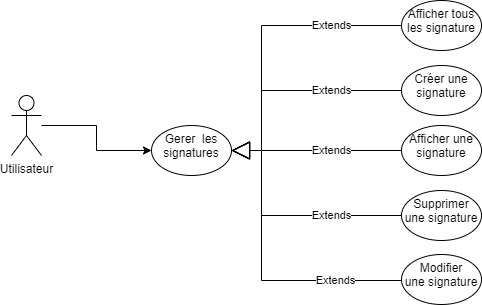
\includegraphics[width=0.8\textwidth]{use_case_signature_sprint_2}
  \caption{Diagramme de cas d'utilisation du sprint 2 : « Gestion des signatures »}
  \label{fig:UseCaseDiagram}
\end{figure}

\subsubsection{Analyse des besoins:}
\textbf{•	Description textuelle de cas d'utilisation « Créer une signature »}

\begin{longtable}{|p{5cm}|p{10cm}|}
\hline
\textbf{Cas d'utilisation}&Créer une signature\\
\hline
\textbf{Acteurs}&Utilisateur\\
\hline
\textbf{Pré Condition}&L'utilisateur doit être authentifié\\
\hline
\textbf{Post Condition}&Création d'une signature\\
\hline
\textbf{Scénario Nominal}&
\vspace{-\baselineskip}
\begin{enumerate}
    \setcounter{enumi}{1}
  \item L'utilisateur dessine sa signature sur le pad.
  \item L'utilisateur clique sur le bouton enregistrer.
  \item Le système affiche un panneau d'ajout de nom.
  \item L'utilisateur entre le nom de la signature.
  \item L'utilisateur clique sur le bouton enregistrer.
  \item Le système enregistre la signature.
  \item Le système affiche un message de succès.
  \item Le system cache le panneau d'ajout de nom.
\end{enumerate}\\
\hline
\textbf{Scénario Alternatif}&
\vspace{-\baselineskip}
\begin{enumerate}
      \item [2.1] L'utilisateur ne dessine pas sa signature sur le pad.
      \item [2.2] Le système affiche un message d'erreur pour s'assurer de dessiner la signature.
      \item [5.1] L'utilisateur ne donne pas de nom à la signature.
      \item [5.2] Le système affiche un message d'erreur pour s'assurer de donner un nom à la signature.
\end{enumerate}\\
\hline
\textbf{Scénario d'exception}&Erreur de connexion\\
\hline
\caption{Description textuelle du diagramme de cas d'utilisation « Créer une signature »}
\label{tab:use_case_create_signature}
\end{longtable}

% \textbf{Terminologie paragraphe :} \\
% \textbf{OCR :} signifie Optical Character Recognition (reconnaissance optique de caractères en français). Il s'agit d'un processus de conversion d'images numérisées de textes en fichiers éditables et interprétables par des ordinateurs.
  

\textbf{•	Description textuelle de cas d'utilisation « Afficher les signatures »}

\begin{longtable}{|p{5cm}|p{10cm}|}
\hline
\textbf{Cas d'utilisation}&Afficher les signatures\\
\hline
\textbf{Acteurs}&Utilisateur \\
\hline
\textbf{Pré Condition}&L'utilisateur doit être authentifié\\
\hline
\textbf{Post Condition}&Affichage des signatures\\
\hline
\textbf{Scénario Nominal}&
\vspace{-\baselineskip}
\begin{enumerate}
    \setcounter{enumi}{1}
    \item L'utilisateur clique sur le bouton « Signatures ».
    \item Le système affiche la liste des signatures.
\end{enumerate}\\
\hline
\textbf{Scénario alternatif}&
\begin{enumerate}
  \item [2.1] L'utilisateur n'a pas de signature.
  \item [2.2] Le système affiche un message pour l'inviter à créer une signature.
\end{enumerate}\\
\hline
\textbf{Scénario d'exception}&Erreur de connexion\\
\hline
\caption{Description textuelle du diagramme de cas d'utilisation « Afficher les signatures »}
\label{tab:use_case_view_signature}
\end{longtable}


\textbf{•	Description textuelle de cas d'utilisation « Supprimer une signature »}

\begin{longtable}{|p{5cm}|p{10cm}|}
\hline
\textbf{Cas d'utilisation}&Supprimer une signature\\
\hline
\textbf{Acteurs}&Utilisateur \\
\hline
\textbf{Pré Condition}&L'utilisateur doit être authentifié et avoir des signatures.\\
\hline
\textbf{Post Condition}&Suppression  d'une signature\\
\hline
\textbf{Scénario Nominal}&
\vspace{-\baselineskip}
\begin{enumerate}
    \setcounter{enumi}{1}
    \item L'utilisateur clique sur le bouton supprimer.
    \item Le système affiche une alerte de vérification.
    \item L'utilisateur clique sur le bouton confirme.
    \item La signature est supprimer de la base.
    \item Le système affiche un message de succès.
\end{enumerate}\\
\hline
\textbf{Scénario d'exception}&Erreur de connexion\\
\hline
\caption{Description textuelle du diagramme de cas d'utilisation « Supprimer une signature »}
\label{tab:use_case_delete_signature}
\end{longtable}


\textbf{•	Description textuelle de cas d'utilisation « Visualiser une signature »}

\begin{longtable}{|p{5cm}|p{10cm}|}
\hline
\textbf{Cas d'utilisation}&Visualiser une signature\\
\hline
\textbf{Acteurs}&Utilisateur \\
\hline
\textbf{Pré Condition}&L'utilisateur doit être authentifié et avoir des signatures.\\
\hline
\textbf{Post Condition}&Visualisation d'une signature\\
\hline
\textbf{Scénario Nominal}&
\vspace{-\baselineskip}
\begin{enumerate}
    \setcounter{enumi}{1}
    \item L'utilisateur clique sur le bouton visualiser.
    \item Le système affiche la signature.
\end{enumerate}\\
\hline
\textbf{Scénario d'exception}&Erreur de connexion\\
\hline
\caption{Description textuelle du diagramme de cas d'utilisation « Visualiser une signature »}
\label{tab:use_case_view_single_signature}
\end{longtable}


\textbf{•	Description textuelle de cas d'utilisation « Créer une signature a l'aide du caméra ou d'image »}
\begin{longtable}{|p{5cm}|p{10cm}|}
\hline
\textbf{Cas d'utilisation}&Créer une signature a l'aide du caméra ou d'image\\
\hline
\textbf{Acteurs}&Utilisateur \\
\hline
\textbf{Pré Condition}&L'utilisateur doit être authentifié.\\
\hline
\textbf{Post Condition}&Création d'une signature\\
\hline
\textbf{Scénario Nominal}&
\vspace{-\baselineskip}
\begin{enumerate}
    \setcounter{enumi}{1}
    \item L'utilisateur clique sur le bouton Importer.
    \item Le système affiche une fenêtre pour choisir ou prendre une image.
    \item L'utilisateur choisit l'image.
    \item Le système affiche l'image pour que l'utilisateur puisse la redimensionner.
    \item L'utilisateur redimensionne l'image.
    \item Le système récupère la signature de la partie de l'image choisie et l'affiche pour que l'utilisateur puisse la modifier.
    \item L'utilisateur modifie la signature.
    \item Le systeme procède à la création de la signature. // TODO !!
\end{enumerate}\\
\hline
\textbf{Scénario alternatif}&
\begin{enumerate}
  \item [2.1] L'utilisateur choisit une fichier qui n'est pas une image.
  \item [2.2] Le système affiche un message d'erreur.
  \item [4.1] L'utilisateur annule la redimension.
  \item [4.2] Le scenario reprend à l'étape 2.
\end{enumerate}\\
\hline
\textbf{Scénario d'exception}&Erreur de connexion\\
\hline
\caption{Description textuelle du diagramme de cas d'utilisation « Créer une signature a l'aide du caméra ou d'image »}
\label{tab:use_case_create_signature_from_image}
\end{longtable}

Pour créer notre plateforme, nous avons pensé qu'il était nécessaire de réaliser une maquette. Les maquettes nous aident à concevoir des interfaces qui répondent aux attentes et aux besoins du client. Elles permettent également de s'assurer que les besoins du client sont adaptés au projet. Nous avons réalisé un prototype de notre système, comme le montrent les figures ci-dessous. Tout au long de notre projet, nous présenterons des maquettes.

\begin{figure}[H]
  \centering
  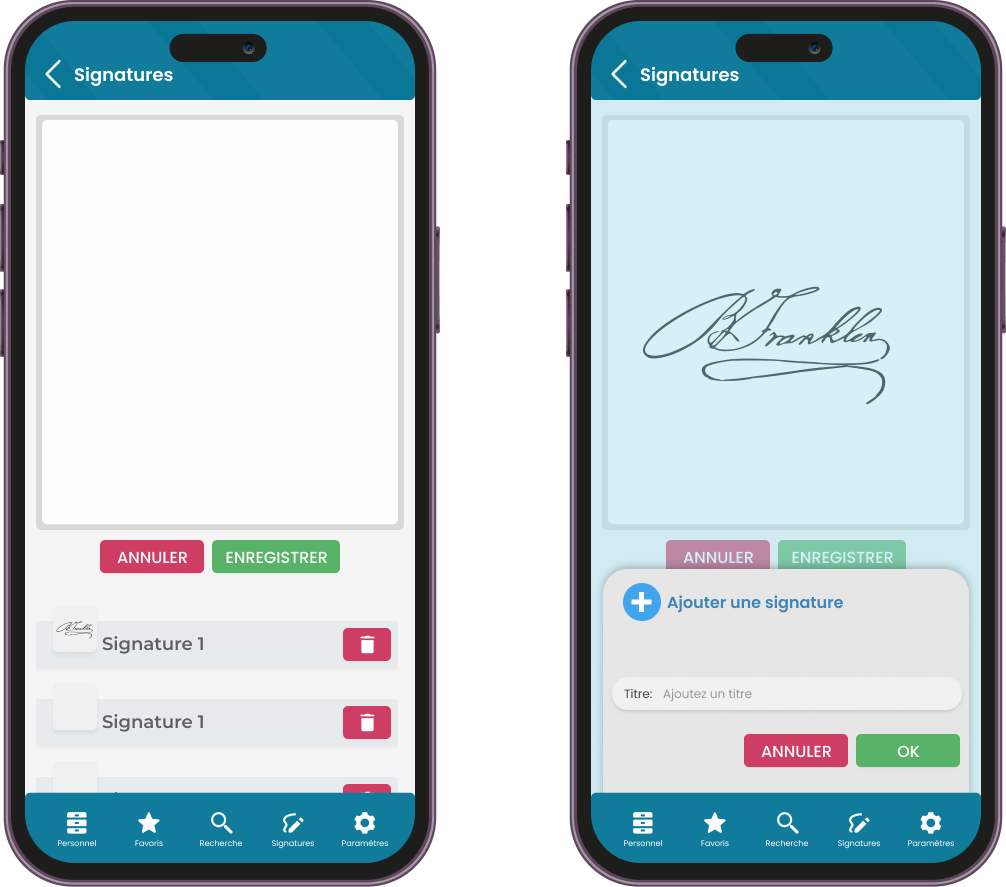
\includegraphics[width=0.7\textwidth]{design_signatures}
  \caption{Maquette de la page des signatures}
  \label{fig:design_signatures}
\end{figure}

\begin{figure}[H]
  \centering
  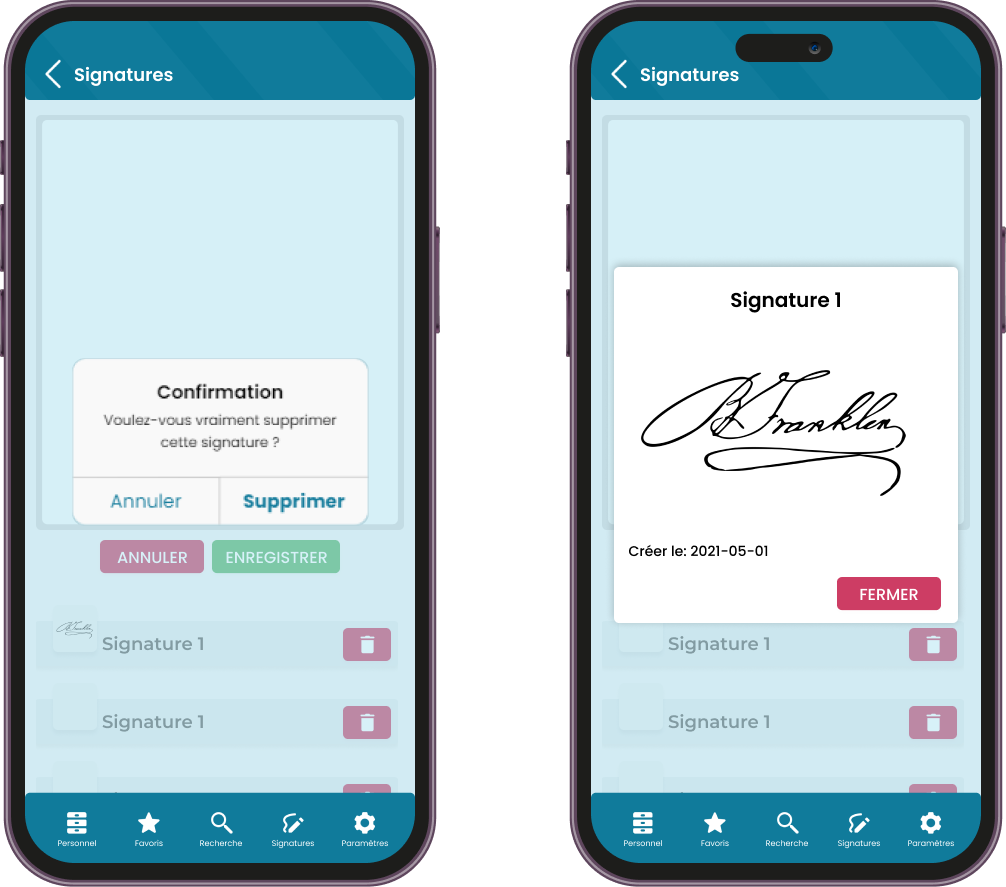
\includegraphics[width=0.7\textwidth]{preview_delete_signature}
  \caption{Maquette de la page de visualisation et de suppression d'une signature}
  \label{fig:design_preview_delete_signature}
\end{figure}

Pour avoir une représentation temporelle des interactions entre les objets de notre système et de la chronologie des messages échangés entre eux et avec les acteurs nous avons réalisé les diagrammes de séquence représentés ci-dessous

\textbf{•	Diagramme de séquence de cas d'utilisation « Créer une signature  »}
\begin{figure}[H]
  \centering
  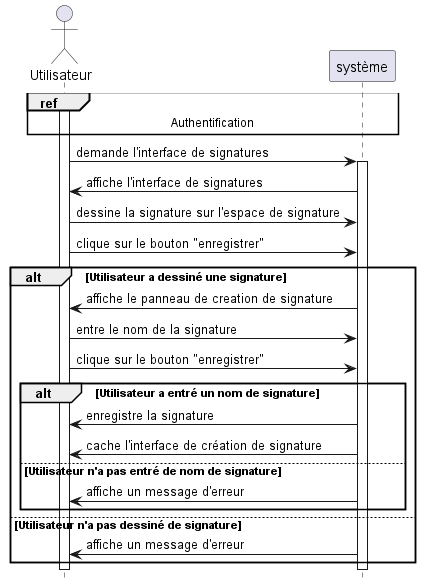
\includegraphics[width=0.7\textwidth]{out/diagrams/signatures/create/create_signature}
  \caption{Diagramme de séquence de cas d'utilisation « Créer une signature  »}
  \label{fig:sequence_create_signature}
\end{figure}

\textbf{•	Diagramme de séquence de cas d'utilisation « Supprimer une signature  »}
\begin{figure}[H]
  \centering
  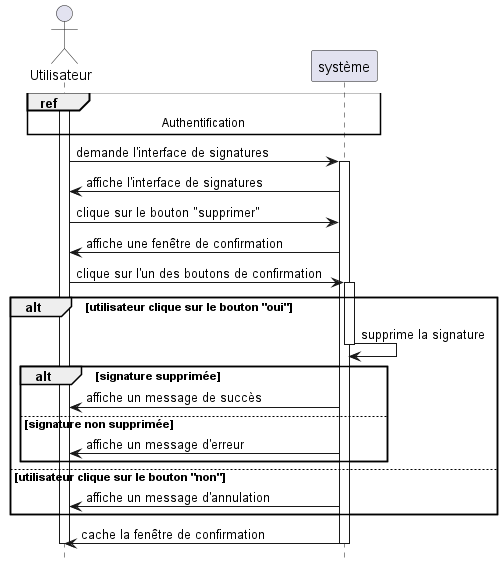
\includegraphics[width=0.7\textwidth]{out/diagrams/signatures/delete/delete_signature}
  \caption{Diagramme de séquence de cas d'utilisation « Supprimer une signature  »}
  \label{fig:sequence_delete_signature}
\end{figure}

\textbf{•	Diagramme de séquence de cas d'utilisation « Visualiser une signature  »}
\begin{figure}[H]
  \centering
  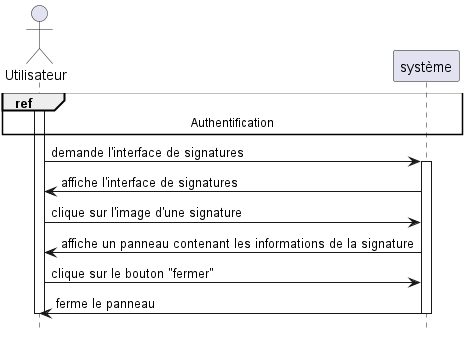
\includegraphics[width=0.7\textwidth]{out/diagrams/signatures/view/view_signature}
  \caption{Diagramme de séquence de cas d'utilisation « Visualiser une signature  »}
  \label{fig:sequence_view_signature}
\end{figure}

\textbf{•	Diagramme de séquence de cas d'utilisation « Modifier une signature  »}
\begin{figure}[H]
  \centering
  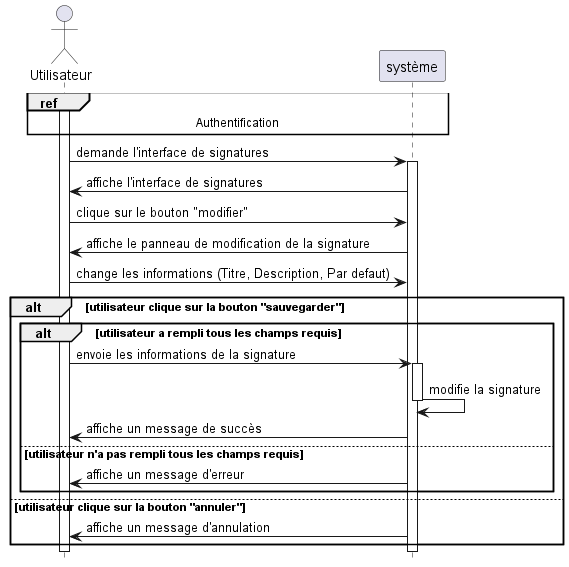
\includegraphics[width=0.7\textwidth]{out/diagrams/signatures/update/update_signature}
  \caption{Diagramme de séquence de cas d'utilisation « Modifier une signature  »}
  \label{fig:sequence_update_signature}
\end{figure}

\subsubsection{Analyse détaillée}
La présentation de démarche d'analyse fonctionnelle d'un sprint est très importante pour la satisfaction d'un client parce qu'elle consiste à caractériser les fonctions offertes par un produit.
Donc, nous allons faire l'analyse des différents cas d'utilisation en utilisant le diagramme de classes d'analyse.

Les objets de diagramme d'analyse sont les suivants :
% View
\begin{itemize}
  \item \textbf{View} : représente la vue de l'application.
  \item \textbf{ViewModel} : représente le modèle de la vue.
  \item \textbf{Model} : représente le modèle de l'application.
  \item \textbf{EliseWebService} : représente le web service de l'application Elise.
\end{itemize}

\textbf{•	Diagramme de classe d'analyse de sprint 2 }
\newpage

\begin{figure}
  \centering
  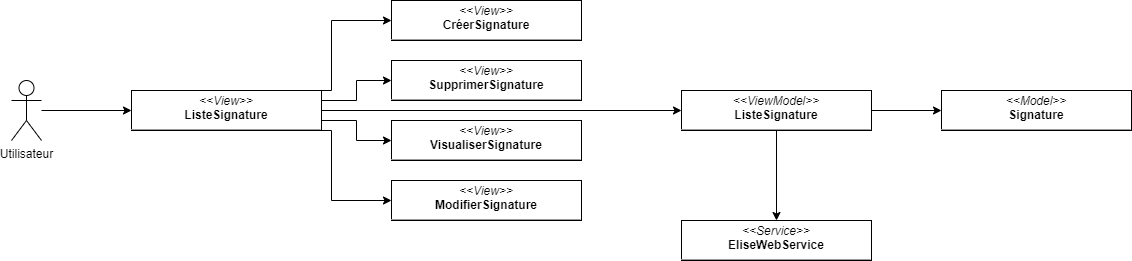
\includegraphics[width=1\textwidth]{dca_sprint2}
  \caption{Diagramme de classe d'analyse de sprint 2}
  \label{fig:class_analyse_signatures}
\end{figure}


\subsubsection{Conception}

Après la présentation des diagrammes d'analyse, nous avons présenté dans cette partie les diagrammes de conception.\\ 
Nous allons présenter dans cette partie les diagrammes de conception de sprint 2. \\
\textbf{•	Diagramme de classe de conception de sprint 2 : « Gestion des signatures »}

% add image
\begin{figure}[H]
  \centering
  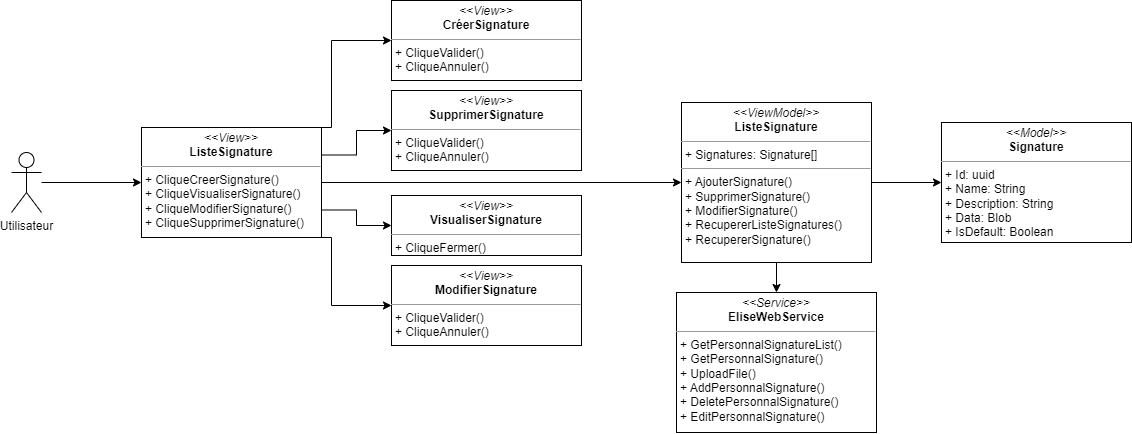
\includegraphics[width=1\textwidth]{dcc_spint2}
  \caption{Diagramme de classe de conception de sprint 2 : « Gestion des signatures »}
  \label{fig:class_diagram_signatures}
\end{figure}


\begin{figure}[H]
  \centering
  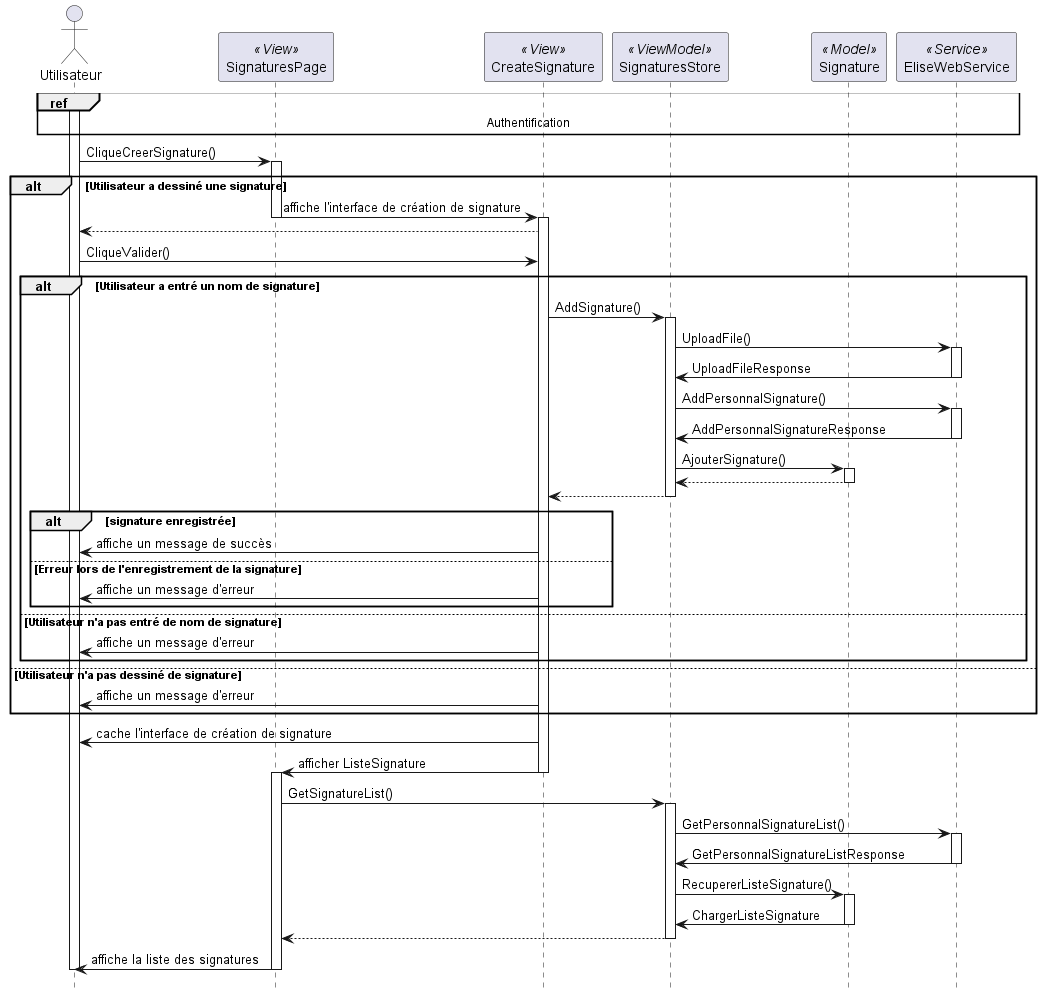
\includegraphics[width=1\textwidth]{out/diagrams/signatures/sequence_create/sequence_create_signature}
  \caption{Diagramme de séquence de conception de cas d'utilisation « Créer une signature  »}
  \label{fig:sequence_conception_create_signature}
\end{figure}

\begin{figure}[H]
  \centering
  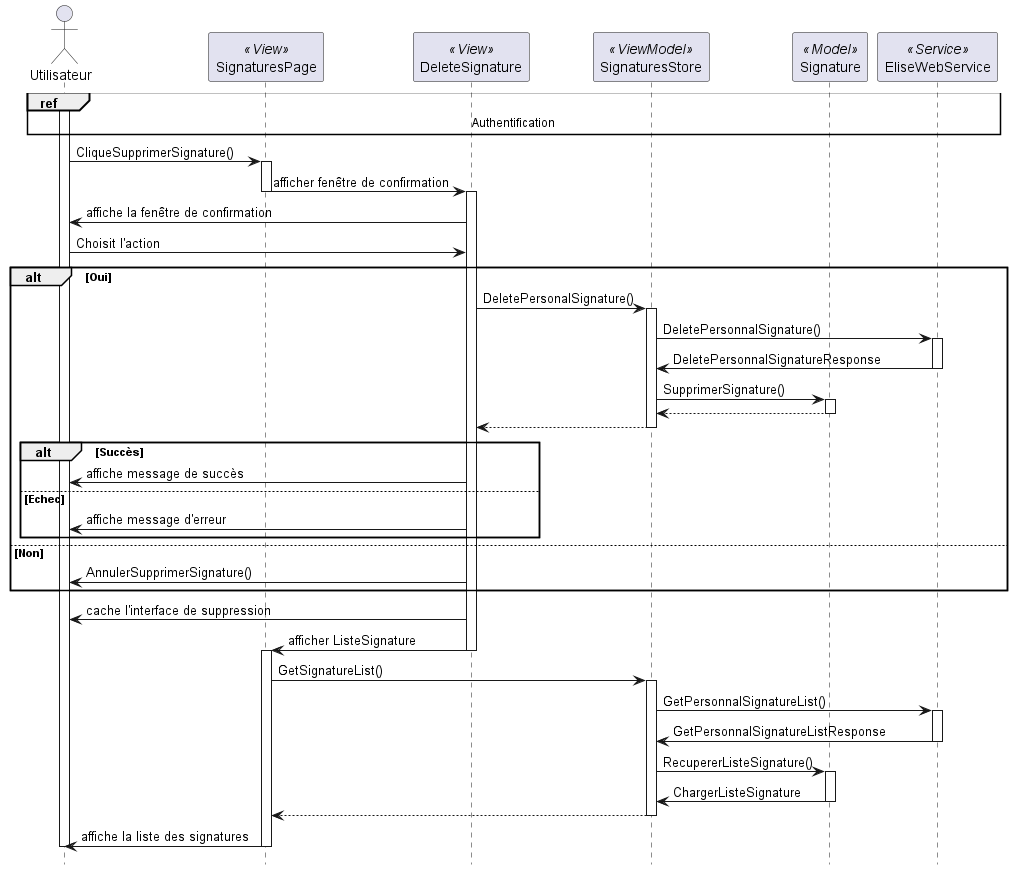
\includegraphics[width=1\textwidth]{out/diagrams/signatures/sequence_delete/sequence_delete_signature}
  \caption{Diagramme de séquence de conception de cas d'utilisation « Supprimer une signature  »}
  \label{fig:sequence_conception_delete_signature}
\end{figure}

\begin{figure}[H]
  \centering
  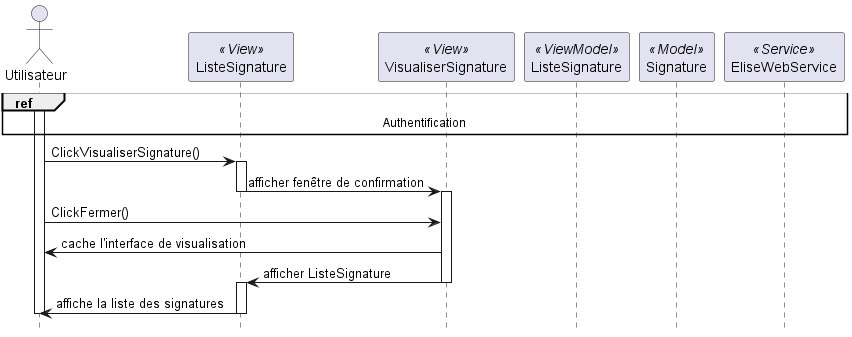
\includegraphics[width=0.7\textwidth]{out/diagrams/signatures/sequence_view/sequence_view_signature}
  \caption{Diagramme de séquence de conception de cas d'utilisation « Visualiser une signature  »}
  \label{fig:sequence_conception_view_signature}
\end{figure}

\begin{figure}[H]
  \centering
  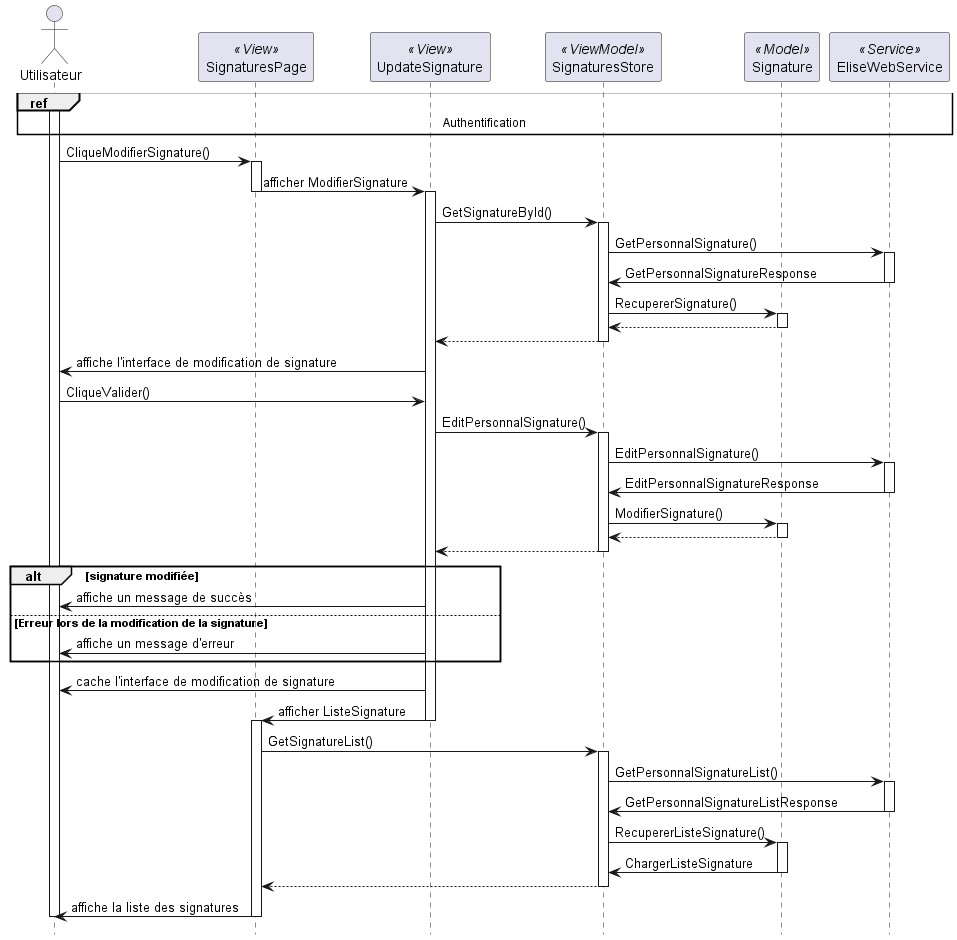
\includegraphics[width=1\textwidth]{out/diagrams/signatures/sequence_update/sequence_update_signature}
  \caption{Diagramme de séquence de conception de cas d'utilisation « Modifier une signature  »}
  \label{fig:sequence_conception_update_signature}
\end{figure}





\subsubsection{Réalisation}

Après la présentation des diagrammes d'analyse, nous avons présenté dans cette partie des captures d'écran de l'application.

\textbf{•	Interface de création d'une signature:}

Cette capture d'écran, représente l'interface de création d'une signature par un utilisateur

% add image
\begin{figure}[H]
  \centering
  \includegraphics[width=0.35\textwidth, height=0.35\textheight,keepaspectratio=true]{signature_creation}
  \caption{Interface de création d'une signature}
  \label{fig:signature_creation}
\end{figure}

\textbf{•	Signer puis cliquer sur « save » : Interface de saisie du titre:}\\
Cette capture d'écran, représente l'interface de saisie du titre de la signature par un utilisateur
% add image
\begin{figure}[H]
  \centering
  \includegraphics[width=0.35\textwidth, height=0.35\textheight,keepaspectratio=true]{signature_form}
  \caption{Interface de saisie du titre de la signature}
  \label{fig:signature_title}
\end{figure}

\textbf{•	Interface de visualisation d'une signature:}\\
Cette capture d'écran, représente l'interface de visualisation d'une signature par un utilisateur

% add image
\begin{figure}[H]
  \centering
  \includegraphics[width=0.35\textwidth, height=0.35\textheight,keepaspectratio=true]{signature_preview}
  \caption{Interface de visualisation d'une signature}
  \label{fig:signature_view}
\end{figure}

\textbf{•	Interface de suppression d'une signature:}\\
Cette capture d'écran, représente l'interface de suppression d'une signature par un utilisateur

% add image
\begin{figure}[h!]
  \centering
  \includegraphics[width=0.35\textwidth, height=0.35\textheight,keepaspectratio=true]{signature_delete}
  \caption{Interface de suppression d'une signature}
  \label{fig:signature_delete}
\end{figure}



\subsection{Sprint Review:}
A la fin de ce sprint, nous avons planifié une réunion dans la société Neoledge afin de vérifier notre démarche de travail par rapport au besoin de client tout en respectant le délai que nous avons prévu.

Nous avons fait une démonstration durant laquelle nous allons présenter notre incrément :

\begin{itemize}
  \item La création d'une signature.
  \item La visualisation de la signature.
  \item La suppression de la signature.
\end{itemize}

\subsection{Sprint retrospective:}

Après la Sprint Review, nous avons réfléchi à des pistes pour améliorer la qualité et l'efficacité de notre application.

\noindent\textbf{•	Ce qui s'est bien passé :}
\begin{itemize}
  \item Nous avons bien partagé les tâches entre nous à travers le logiciel Azure DevOps. 
  \item Nous avons terminé le sprint dans le délai.
\end{itemize}

\noindent\textbf{•	Ce qui s'est mal passé :}
\begin{itemize}
  \item L'intégration du bibliothèque vue-signature-pad
  \item Un problème rencontré lors de la sauvegarde de la signature était que l'image enregistrée occupait la totalité de l'espace du pad, ce qui nécessitait ensuite une étape de découpe pour obtenir uniquement la partie signée.
\end{itemize}

% sprint =3
\section{Sprint 3 « Gestion des documents »}
\subsection{Sprint Goal:}

L'objectif de ce sprint est de développer et mettre en place un système de gestion des documents permettant aux utilisateurs de consulter les informations du document, consulter et gérer un fichier dans un document, consulter et gérer les tâches dans un document, chercher un document et consulter la liste des documents en favoris

\pagebreak

\subsection{Sprint Backlog « Gestion des documents »}

\begin{longtable}{|p{4cm}|p{7cm}|p{2cm}|p{2cm}|}
  \hline
  \textbf{Les items} &\textbf{Les tâches} & \textbf{Période} & \textbf{Sprint} \\
  \hline
  \vspace{-\baselineskip}
  \begin{enumerate}
    \setcounter{enumi}{1}
    \itemsep0em 
      \item Accéder à un document.
      \item Consulter la liste des fichiers d'un document
      \item Ajoutez un fichier à un document.
      % \item Supprimer un fichier d'un document.
      \item Consulter la liste des tâches d'un document.
      % \item Démarrer une tâche.
      \item Transférer une tâche.
      \item Terminer une tâche.
      \item Consulter la liste des documents en favoris.
      \item Chercher un document.
      

  \end{enumerate}
  &
  \vspace{-\baselineskip}
  \begin{itemize}
    \itemsep0em 
    \item Préparer les interfaces sur Figma.
    \item Développer l'interface des favoris.
    \item Développer l'interface des documents.
    \item Développer l'interface de recherche de documents.
    \item Développer l'interface de liste des fichiers.
    \item Développer l'interface de liste des tâches.
    \item Développer une fonction qui permet de récupérer la liste des documents d'une base de donner.
    \item Développer une fonction qui permet de récupérer la liste des documents en favoris.
    \item Développer une fonction qui permet de chercher un document.
    \item Développer une fonction qui permet ajouter un fichier à un document.
    \item Développer une fonction qui permet de supprimer un fichier.
    \item Développer une fonction qui permet de démarrer une tâche d'un document.
    \item Développer une fonction qui permet de transférer une tâche.
    \item Développé une fonction qui permet de terminer une tâche.

  \end{itemize}
  &
  De 8 à 15 février  
  &
  3
  \\
  \hline
  \caption{Product Backlog Sprint 3}
  \label{tab:product_backlog_sprint_3}



\end{longtable}


\subsection{Implémentation du Sprint 3}
\textbf{•	Diagramme de cas d'utilisation du sprint 3 : « Gestion des documents »}

% add image
\begin{figure}[H]
  \centering
  \includegraphics[width=0.8\textwidth]{use_case_documents_sprint_3}
  \caption{Diagramme de cas d'utilisation du sprint 3 : « Gestion des documents »}
  \label{fig:UseCaseDiagramSprint3}
\end{figure}


\subsubsection{Analyse des besoins:}
\textbf{•	Description textuelle de cas d'utilisation « Accéder à un document »}

\begin{longtable}{|p{5cm}|p{10cm}|}
\hline
\textbf{Cas d'utilisation}&Accéder à un document\\
\hline
\textbf{Acteurs}&Utilisateur\\
\hline
\textbf{Pré Condition}&Le document existe\\
\hline
\textbf{Post Condition}&Consultation d'un document\\
\hline
\textbf{Scénario Nominal}&
\vspace{-\baselineskip}
\begin{enumerate}
    \setcounter{enumi}{1}
    \item L'utilisateur clique sur le document.
    \item Le système affiche l'interface de document.
    
\end{enumerate}\\
\hline
\textbf{Scénario Alternatif}&
\vspace{-\baselineskip}
\begin{enumerate}
    \setcounter{enumi}{2}
    \item Aucun résultat.
\end{enumerate}\\
\hline
\textbf{Scénario d'exception}&Erreur de connexion\\
\hline
\end{longtable}


\textbf{•	Description textuelle de cas d'utilisation « consulter la liste des fichiers d'un document »}

\begin{longtable}{|p{5cm}|p{10cm}|}
\hline
\textbf{Cas d'utilisation}&Consulter la liste des fichiers d'un document\\
\hline
\textbf{Acteurs}&Utilisateur\\
\hline
\textbf{Pré Condition}&Le document existe\\
\hline
\textbf{Post Condition}&Consultation de la liste des fichiers\\
\hline
\textbf{Scénario Nominal}&
\vspace{-\baselineskip}
\begin{enumerate}
    \setcounter{enumi}{1}
    \item L'utilisateur clique sur le bouton fichier.
    \item Le système affiche l'interface de la liste des fichiers.
    
\end{enumerate}\\
\hline
\textbf{Scénario Alternatif}&
\vspace{-\baselineskip}
\begin{enumerate}
    \setcounter{enumi}{2}
    \item Aucun résultat.
\end{enumerate}\\
\hline
\textbf{Scénario d'exception}&Erreur de connexion\\
\hline
\end{longtable}

\textbf{•	Description textuelle de cas d'utilisation « ajouter un fichier à un document »}

\begin{longtable}{|p{5cm}|p{10cm}|}
\hline
\textbf{Cas d'utilisation}&Ajouter un fichier à un document\\
\hline
\textbf{Acteurs}&Utilisateur\\
\hline
\textbf{Pré Condition}&Le document existe\\
\hline
\textbf{Post Condition}&Fichier ajouté\\
\hline
\textbf{Scénario Nominal}&
\vspace{-\baselineskip}
\begin{enumerate}
    \setcounter{enumi}{1}
    \item L'utilisateur clique sur le bouton ajouter.
    \item Le système affiche l'interface d'ajout des fichiers.
    \item L'utilisateur ajoute le fichier et clique sur le bouton confirmer.
    \item le système affiche un message des succès.
    
    
\end{enumerate}\\
\hline
\textbf{Scénario Alternatif}&
\vspace{-\baselineskip}
\begin{enumerate}
    \setcounter{enumi}{3}
    \item L'utilisateur annule l'ajout du fichier.
\end{enumerate}\\
\hline
\textbf{Scénario d'exception}&Erreur de connexion\\
\hline
\end{longtable}


% \textbf{•	Description textuelle de cas d'utilisation « supprimer un fichier dans un document »}

% \begin{longtable}{|p{5cm}|p{10cm}|}
% \hline
% \textbf{Cas d'utilisation}&Supprimer un fichier d'un document\\
% \hline
% \textbf{Acteurs}&Utilisateur\\
% \hline
% \textbf{Pré Condition}&Le document existe\\
% \hline
% \textbf{Post Condition}&Fichier supprimé\\
% \hline
% \textbf{Scénario Nominal}&
% \vspace{-\baselineskip}
% \begin{enumerate}
%     \setcounter{enumi}{1}
%     \item L'utilisateur clique sur le bouton supprimer.
%     \item Le système affiche une alerte de confirmation.
%     \item L'utilisateur clique sur le bouton confirmer.
%     \item le système supprime le fichier et affiche un message des succès.
    
    
    
% \end{enumerate}\\
% \hline
% \textbf{Scénario Alternatif}&
% \vspace{-\baselineskip}
% \begin{enumerate}
%     \setcounter{enumi}{3}
%     \item L'utilisateur annule la suppression du fichier.
% \end{enumerate}\\
% \hline
% \textbf{Scénario d'exception}&Erreur de connexion\\
% \hline
% \end{longtable}



\textbf{•	Description textuelle de cas d'utilisation « consulter la liste des tâches d'un document »}

\begin{longtable}{|p{5cm}|p{10cm}|}
\hline
\textbf{Cas d'utilisation}&Consulter la liste des tâches d'un document\\
\hline
\textbf{Acteurs}&Utilisateur\\
\hline
\textbf{Pré Condition}&Le document existe\\
\hline
\textbf{Post Condition}&Consultation des tâches\\
\hline
\textbf{Scénario Nominal}&
\vspace{-\baselineskip}
\begin{enumerate}
    \setcounter{enumi}{1}
    \item L'utilisateur clique sur le bouton tâches.
    \item Le système affiche l'interface de la liste des tâches.
    
\end{enumerate}\\
\hline
\textbf{Scénario Alternatif}&
\vspace{-\baselineskip}
\begin{enumerate}
    \setcounter{enumi}{3}
    \item Aucun tâche trouvée.
\end{enumerate}\\
\hline
\textbf{Scénario d'exception}&Erreur de connexion\\
\hline
\end{longtable}



\textbf{•	Description textuelle de cas d'utilisation « Demander une tâche »}

\begin{longtable}{|p{5cm}|p{10cm}|}
\hline
\textbf{Cas d'utilisation}&Demander une tâche\\
\hline
\textbf{Acteurs}&Utilisateur\\
\hline
\textbf{Pré Condition}&La document a au moins une tâche\\
\hline
\textbf{Post Condition}&Tâche demandée\\
\hline
\textbf{Scénario Nominal}&
\vspace{-\baselineskip}
\begin{enumerate}
    \setcounter{enumi}{1}
    \item L'utilisateur clique sur le bouton demander.
    \item Le système affiche un modal de demande de tâche.
    \item L'utilistauer rempli le formulaire.
    \item L'utilisateur clique sur le bouton confirmer.
    \item Le système cache le modal de demande de tâche.
    \item Le système affiche un message de succès.
\end{enumerate}\\
\hline
\textbf{Scénario Alternatif}&
\vspace{-\baselineskip}
\begin{enumerate}
    \setcounter{enumi}{4}
    \item L'utilisateur annule la demande de tâche.
    \item Le système cache le modal de demande de tâche.
\end{enumerate}\\
\hline
\textbf{Scénario d'exception}&Erreur de connexion\\
\hline
\end{longtable}


\textbf{•	Description textuelle de cas d'utilisation « Tranférer une tâche »}

\begin{longtable}{|p{5cm}|p{10cm}|}
\hline
\textbf{Cas d'utilisation}&Tranférer une tâche\\
\hline
\textbf{Acteurs}&Utilisateur\\
\hline
\textbf{Pré Condition}&La document a au moins une tâche\\
\hline
\textbf{Post Condition}&Tâche transférée\\
\hline
\textbf{Scénario Nominal}&
\vspace{-\baselineskip}
\begin{enumerate}
    \setcounter{enumi}{1}
    \item L'utilisateur clique sur le bouton transférer.
    \item Le système affiche un modal de transfert de tâche.
    \item L'utilistauer rempli le formulaire.
    \item L'utilisateur clique sur le bouton confirmer.
    \item Le système cache le modal de transfert de tâche.
    \item Le système affiche un message de succès.
\end{enumerate}\\
\hline
\textbf{Scénario Alternatif}&
\vspace{-\baselineskip}
\begin{enumerate}
    \setcounter{enumi}{4}
    \item L'utilisateur annule la transfert de tâche.
    \item Le système cache le modal de transfert de tâche.
\end{enumerate}\\
\hline
\textbf{Scénario d'exception}&Erreur de connexion\\
\hline
\end{longtable}

\textbf{•	Description textuelle de cas d'utilisation « Terminer une tâche »}

\begin{longtable}{|p{5cm}|p{10cm}|}
\hline
\textbf{Cas d'utilisation}&Terminer une tâche\\
\hline
\textbf{Acteurs}&Utilisateur\\
\hline
\textbf{Pré Condition}&La document a au moins une tâche\\
\hline
\textbf{Post Condition}&Tâche terminée\\
\hline
\textbf{Scénario Nominal}&
\vspace{-\baselineskip}
\begin{enumerate}
    \setcounter{enumi}{1}
    \item L'utilisateur clique sur le bouton terminer.
    \item Le système affiche un modal de confirmation de terminaison de tâche.
    \item L'utilisateur clique sur le bouton confirmer.
    \item Le système cache le modal de confirmation de terminaison de tâche.
    \item Le système affiche un message de succès.
\end{enumerate}\\
\hline
\textbf{Scénario Alternatif}&
\vspace{-\baselineskip}
\begin{enumerate}
    \setcounter{enumi}{4}
    \item L'utilisateur annule la terminaison de tâche.
    \item Le système cache le modal de confirmation de terminaison de tâche.
\end{enumerate}\\
\hline
\textbf{Scénario d'exception}&Erreur de connexion\\
\hline
\end{longtable}



\textbf{•	Description textuelle de cas d'utilisation « Consulter la liste des documents en favoris  »}

\begin{longtable}{|p{5cm}|p{10cm}|}
\hline
\textbf{Cas d'utilisation}&Consulter la liste des documents en favoris\\
\hline
\textbf{Acteurs}&Utilisateur\\
\hline
\textbf{Pré Condition}&L'utilisateur a au moins un document en favoris\\
\hline
\textbf{Post Condition}&Affichage de la liste des documents en favoris\\
\hline
\textbf{Scénario Nominal}&
\vspace{-\baselineskip}
\begin{enumerate}
    \setcounter{enumi}{1}
    \item L'utilisateur clique sur le bouton favoris.
    \item Le système affiche la liste des documents en favoris.
\end{enumerate}\\
\hline
\textbf{Scénario Alternatif}&
\vspace{-\baselineskip}
\begin{enumerate}
    \setcounter{enumi}{2}
    \item Aucun document en favoris.
\end{enumerate}\\
\hline
\textbf{Scénario d'exception}&Erreur de connexion\\
\hline
\end{longtable}




\textbf{•	Description textuelle de cas d'utilisation « Chercher un document »}

\begin{longtable}{|p{5cm}|p{10cm}|}
\hline
\textbf{Cas d'utilisation}&Chercher un document\\
\hline
\textbf{Acteurs}&Utilisateur\\
\hline
\textbf{Pré Condition}&\\
\hline
\textbf{Post Condition}&Liste des documents correspondant à la recherche\\
\hline
\textbf{Scénario Nominal}&
\vspace{-\baselineskip}
\begin{enumerate}
    \setcounter{enumi}{1}
    \item L'utilisateur clique sur le bouton rechercher.
    \item Le système affiche l'inteface de recherche des documents.
    \item L'utilisateur rempli le formulaire de recherche.
    \item Le système affiche la liste des documents correspondant à la recherche.
\end{enumerate}\\
\hline
\textbf{Scénario Alternatif}&
\vspace{-\baselineskip}
\begin{enumerate}
    \setcounter{enumi}{4}
    \item Aucun document correspondant à la recherche.
\end{enumerate}\\
\hline
\textbf{Scénario d'exception}&Erreur de connexion\\
\hline
\end{longtable}


% Add sequence system
\textbf{•	Diagramme de séquence de cas d'utilisation « Accéder à un document  »}
\begin{figure}[H]
  \centering
  \includegraphics[width=0.7\textwidth]{out/diagrams/documents/preview/preview_document}
  \caption{Diagramme de séquence de cas d'utilisation « Accéder à un document  »}
  \label{fig:sequence_Accederaundocument}
\end{figure}
\textbf{•	Diagramme de séquence de cas d'utilisation « Consulter la liste des fichiers d'un document  »}
\begin{figure}[H]
  \centering
  \includegraphics[width=0.7\textwidth]{out/diagrams/documents/previewFiles/preview_files_document}
  \caption{Diagramme de séquence de cas d'utilisation « Consulter la liste des fichiers d'un document  »}
  \label{fig:sequence_previewFiles}
\end{figure}
\textbf{•	Diagramme de séquence de cas d'utilisation « Consulter la liste des tâches d'un document  »}
\begin{figure}[H]
  \centering
  \includegraphics[width=0.7\textwidth]{out/diagrams/documents/previewTasks/preview_tasks_document}
  \caption{Diagramme de séquence de cas d'utilisation « Consulter la liste des tâches d'un document  »}
  \label{fig:sequence_previewTasks}
\end{figure}
\textbf{•	Diagramme de séquence de cas d'utilisation « Transferer une tâche  »}
\begin{figure}[H]
  \centering
  \includegraphics[width=1\textwidth]{out/diagrams/documents/transfer_task/transfer_task}
  \caption{Diagramme de séquence de cas d'utilisation « Transferer une tâche  »}
  \label{fig:sequence_transfer_task}
\end{figure}
\textbf{•	Diagramme de séquence de cas d'utilisation « Terminer une tâche  »}
\begin{figure}[H]
  \centering
  \includegraphics[width=1\textwidth]{out/diagrams/documents/terminer_task/terminer_task}
  \caption{Diagramme de séquence de cas d'utilisation « Terminer une tâche  »}
  \label{fig:sequence_terminer_task}
\end{figure}
\textbf{•	Diagramme de séquence de cas d'utilisation « Ajoutez un fichier à un document  »}
\begin{figure}[H]
  \centering
  \includegraphics[width=1\textwidth]{out/diagrams/documents/add_file/add_file}
  \caption{Diagramme de séquence de cas d'utilisation « Ajoutez un fichier à un document  »}
  \label{fig:sequence_add_file}
\end{figure}
\textbf{•	Diagramme de séquence de cas d'utilisation « Consulter la liste des documents en favoris  »}
\begin{figure}[H]
  \centering
  \includegraphics[width=0.7\textwidth]{out/diagrams/documents/favoris/favorit_document}
  \caption{Diagramme de séquence de cas d'utilisation « Consulter la liste des documents en favoris  »}
  \label{fig:sequence_favorit_document}
\end{figure}
\textbf{•	Diagramme de séquence de cas d'utilisation « Chercher un document  »}
\begin{figure}[H]
  \centering
  \includegraphics[width=0.7\textwidth]{out/diagrams/documents/chercher/charcher_document}
  \caption{Diagramme de séquence de cas d'utilisation « Chercher un document  »}
  \label{fig:sequence_charcher_document}
\end{figure}

\subsubsection{Analyse détaillée}
\textbf{•	Diagramme de classe d'analyse de sprint "3" }
\newpage

\begin{figure}
  \centering
  \includegraphics[width=1\textwidth]{dca_sprint3}
  \caption{Diagramme de classe d'analyse de sprint 3}
  \label{fig:class_analyse_signatures3}
\end{figure}


\subsubsection{Conception}

Après la présentation des diagrammes d'analyse, nous avons présenté dans cette partie les diagrammes de conception.
Nous allons présenter dans cette partie les diagrammes de conception de sprint 3.
\newpage 
\begin{landscape}

\textbf{•	Diagramme de classe de conception de sprint 3 : « Gestion des documents »}

\begin{figure}[H]
  \centering
  \includegraphics[height=0.8\textheight]{dcc_spint3}
  \caption{Diagramme de classe de conception de sprint 3 : « Gestion des signatures »}
  \label{fig:class_diagram_signatures3}
\end{figure}
\end{landscape}
\newpage
\begin{figure}[H]
  \centering
  \includegraphics[width=1\textwidth]{out/diagrams/documents/sequence_preview/sequence_preview}
  \caption{Diagramme de séquence de conception de cas d'utilisation « Accéder à un document »}
  \label{fig:sequence_conception_preview_document}
\end{figure}
\begin{figure}[H]
  \centering
  \includegraphics[width=1\textwidth]{out/diagrams/documents/sequence_preview_files/sequence_preview_files}
  \caption{Diagramme de séquence de conception de cas d'utilisation « Consulter la liste des fichiers d'un document »}
  \label{fig:sequence_conception_previewFiles}
\end{figure}
\begin{figure}[H]
  \centering
  \includegraphics[width=1\textwidth]{out/diagrams/documents/sequence_preview_tasks/sequence_preview_tasks}
  \caption{Diagramme de séquence de conception de cas d'utilisation « Consulter la liste des tâches d'un document »}
  \label{fig:sequence_conception_previewTasks}
\end{figure}
\begin{figure}[H]
  \centering
  \includegraphics[width=1\textwidth]{out/diagrams/documents/sequence_transfer_task/sequence_transfer_task}
  \caption{Diagramme de séquence de conception de cas d'utilisation « Transferer une tâche »}
  \label{fig:sequence_conception_transferTask}
\end{figure}
\begin{figure}[H]
  \centering
  \includegraphics[width=1\textwidth]{out/diagrams/documents/sequence_terminer_task/sequence_terminer_task}
  \caption{Diagramme de séquence de conception de cas d'utilisation « Terminer une tâche »}
  \label{fig:sequence_conception_terminerTask}
\end{figure}
\begin{figure}[H]
  \centering
  \includegraphics[width=1\textwidth]{out/diagrams/documents/sequence_add_file/sequence_add_file}
  \caption{Diagramme de séquence de conception de cas d'utilisation « Ajoutez un fichier à un document »}
  \label{fig:sequence_conception_addFile}
\end{figure}
\begin{figure}[H]
  \centering
  \includegraphics[width=1\textwidth]{out/diagrams/documents/sequence_favoris/sequence_favoris}
  \caption{Diagramme de séquence de conception de cas d'utilisation « Consulter la liste des documents en favoris »}
  \label{fig:sequence_conception_favoritDocument}
\end{figure}
\begin{figure}[H]
  \centering
  \includegraphics[width=1\textwidth]{out/diagrams/documents/sequence_chercher/sequence_chercher}
  \caption{Diagramme de séquence de conception de cas d'utilisation « Chercher un document »}
  \label{fig:sequence_conception_charcherDocument}
\end{figure}

\subsubsection{Réalisation}

Après la présentation des diagrammes d'analyse, nous avons présenté dans cette partie des captures d'écran de l'application.

\textbf{•	Accès aux documents:}

Cette capture d'écran, représente l'interface d'accès aux documents par un utilisateur

% add image
\begin{figure}[H]
  \centering
  \includegraphics[width=0.35\textwidth, height=0.35\textheight,keepaspectratio=true]{acces_aux_document}
  \caption{Interface d'accès aux documents}
  \label{fig:acces_aux_document}
\end{figure}

\textbf{•	Consulter les fichiers d'un document:}

Cette capture d'écran, représente l'interface de consultation des fichiers d'un document par un utilisateur

% add image
\begin{figure}[H]
  \centering
  \includegraphics[width=0.35\textwidth, height=0.35\textheight,keepaspectratio=true]{consult_document_files}
  \caption{Interface de consultation des fichiers d'un document}
  \label{fig:consult_document_files}
\end{figure}

\textbf{•	Consulter les tâches d'un document:}

Cette capture d'écran, représente l'interface de consultation des tâches d'un document par un utilisateur

% add image
\begin{figure}[H]
  \centering
  \includegraphics[width=0.35\textwidth, height=0.35\textheight,keepaspectratio=true]{consult_document_tasks}
  \caption{Interface de consultation des tâches d'un document}
  \label{fig:consult_document_tasks}
\end{figure}

\textbf{•	Ajout de fichiers à un document:}

Cette capture d'écran, représente l'interface d'ajout de fichiers à un document par un utilisateur

% add image
\begin{figure}[H]
  \centering
  \includegraphics[width=0.35\textwidth, height=0.35\textheight,keepaspectratio=true]{add_document_files}
  \caption{Interface d'ajout de fichiers à un document}
  \label{fig:add_document_files}
\end{figure}

\textbf{• Suppression de fichiers d'un document:}

Cette capture d'écran, représente l'interface de suppression de fichiers d'un document par un utilisateur

% add image
\begin{figure}[H]
  \centering
  \includegraphics[width=0.35\textwidth, height=0.35\textheight,keepaspectratio=true]{delete_document_files}
  \caption{Interface de suppression de fichiers d'un document}
  \label{fig:delete_document_files}
\end{figure}


\textbf{•	Recherche d'un document:}

Cette capture d'écran, représente l'interface de recherche d'un document par un utilisateur

% add image
\begin{figure}[H]
  \centering
  \includegraphics[width=0.35\textwidth, height=0.35\textheight,keepaspectratio=true]{search_document}
  \caption{Interface de recherche d'un document}
  \label{fig:search_document}
\end{figure}

\textbf{•	Consulter les documents en favoris:}

Cette capture d'écran, représente l'interface de consultation des documents en favoris par un utilisateur

% add image
\begin{figure}[H]
  \centering
  \includegraphics[width=0.35\textwidth, height=0.35\textheight,keepaspectratio=true]{consult_favoris_documents}
  \caption{Interface de consultation des documents en favoris}
  \label{fig:consult_favoris_documents}
\end{figure}

\textbf{•	Demander une tâche:}

Cette capture d'écran, représente l'interface de demande d'une tâche par un utilisateur

% add image
\begin{figure}[H]
  \centering
  \includegraphics[width=0.35\textwidth, height=0.35\textheight,keepaspectratio=true]{ask_task}
  \caption{Interface de demande d'une tâche}
  \label{fig:ask_task}
\end{figure}

\textbf{•	Transférer une tâche:}

Cette capture d'écran, représente l'interface de transfert d'une tâche par un utilisateur

% add image
\begin{figure}[H]
  \centering
  \includegraphics[width=0.35\textwidth, height=0.35\textheight,keepaspectratio=true]{transfer_task}
  \caption{Interface de transfert d'une tâche}
  \label{fig:transfer_task}
\end{figure}

\textbf{•	Terminaison d'une tâche dans un document:}

Cette capture d'écran, représente l'interface de terminaison d'une tâche dans un document par un utilisateur

% add image
\begin{figure}[H]
  \centering
  \includegraphics[width=0.35\textwidth, height=0.35\textheight,keepaspectratio=true]{end_task}
  \caption{Interface de terminaison d'une tâche dans un document}
  \label{fig:end_task}
\end{figure}




\subsection{Sprint Review:}
A la fin de ce sprint, nous avons planifié une réunion dans la société Neoledge avec le vise avis à Lille, France afin de vérifier notre démarche de travail par rapport au besoin de client tout en respectant le délai que nous avons prévu.
Nous avons fait une démonstration durant laquelle nous allons présenter notre incrément :
\begin{itemize}
  \item La consultation d'un document.
  \item La gestion des fichiers d'un document.
  \item La gestion des taches d'un document.
  \item La recherche d'un document.
  \item La consultation de la liste des documents en favoris.
\end{itemize}

\subsection{Sprint Retrospective:}

Après la Sprint Review, nous avons réfléchi à des pistes pour améliorer la qualité et l'efficacité de notre application.
\noindent\textbf{•	Ce qui a bien passé :}
Nous avons terminé le sprint dans le délai.
\noindent\textbf{•	Ce qui s'est mal passé :}
Manque de documentation de l'ionic 


% SPrint 4 visualisation et signature d'un fichier
\section{Sprint 4 (Visualisation et signature d'un fichier)}
\subsection{Sprint Goal:}
L'objectif de ce sprint est de développer et mettre en place un système de visualisation et signature d'un fichier permettant aux utilisateurs de consulter le fichier et le signer par plusieurs méthodes.


\subsection{Sprint Backlog « Visualisation et signature d'un fichier »:}

\begin{longtable}{|p{4cm}|p{7cm}|p{2cm}|p{2cm}|}
  \hline
  \textbf{Les items} &\textbf{Les tâches} & \textbf{Période} & \textbf{Sprint} \\
  \hline
  \vspace{-\baselineskip}
  \begin{enumerate}
    \setcounter{enumi}{1}
    \itemsep0em 
      \item Visualiser un fichier
      \item Signer à main un fichier
      \item Signé par glisser et déposer une image dans un fichier.
      \item Modifier la position d'une signature d'un fichier.
      \item Supprimer une signature dans fichier.
      \item Confirmer ou annuler la signature d'un fichier
  \end{enumerate}
  &
  \vspace{-\baselineskip}
  \begin{itemize}
    \itemsep0em 
    \item Préparer les interfaces sur Figma.
    \item Développer l'interface de visualisation d'un fichier.
    \item Développer un package neo-pdf-viewer qui permet d'afficher un fichier PDF à partir d'une base 64
    \item Publier le package.
    \item Intégrer le package dans notre projet.
    \item Développer une fonction qui permet de signer un main un fichier
    \item Développer le panel qui contient la liste des signatures
    \item Développer une fonction qui permet de signer par glisser et déposer une image dans un fichier.
    \item Développer une fonction qui permet de modifier la position d'une signature d'un fichier
    \item Développer une fonction qui permet de supprimer une signature d'un fichier.
    \item Développer une fonction qui permet de confirmer ou annuler la signature d'un fichier


  \end{itemize}
  &
  De 8 à 15 février  
  &
  4
  \\
  \hline
  \caption{Product Backlog Sprint 4}
  \label{tab:product_backlog_sprint_4}



\end{longtable}


\subsection{Implémentation du Sprint 4}
\textbf{•	Diagramme de cas d'utilisation du sprint 4 : « Visualisation et signature d'un fichier »}

% add image
\begin{figure}[H]
  \centering
  \includegraphics[width=0.8\textwidth]{use_case_documents_sprint_4}
  \caption{Diagramme de cas d'utilisation du sprint 4 : « Visualisation et signature d'un fichier »}
  \label{fig:UseCaseDiagram}
\end{figure}

\subsubsection{Analyse des besoins:}
\textbf{•	Description textuelle de cas d'utilisation « visualiser un fichier  »}

\begin{longtable}{|p{5cm}|p{10cm}|}
\hline
\textbf{Cas d'utilisation}&Visualiser un fichier\\
\hline
\textbf{Acteurs}&Utilisateur\\
\hline
\textbf{Pré Condition}&Le fichier existe\\
\hline
\textbf{Post Condition}&Le fichier est visualisé\\
\hline
\textbf{Scénario Nominal}&
\vspace{-\baselineskip}
\begin{enumerate}
    \setcounter{enumi}{1}
  \item L'utilisateur clique sur le fichier.
  \item le système affiche le fichier.
\end{enumerate}\\
\hline
\textbf{Scénario Alternatif}&
\vspace{-\baselineskip}
\begin{enumerate}
    \setcounter{enumi}{2}
    \item Aucun résultat.
\end{enumerate}\\
\hline
\textbf{Scénario d'exception}&Erreur de connexion\\
\hline
\end{longtable}

\textbf{•	Description textuelle de cas d'utilisation « Signer à main un fichier »}

\begin{longtable}{|p{5cm}|p{10cm}|}
\hline
\textbf{Cas d'utilisation}&Signer à main un fichier\\
\hline
\textbf{Acteurs}&Utilisateur\\
\hline
\textbf{Pré Condition}&Le fichier existe\\
\hline
\textbf{Post Condition}&La signature est tracée\\
\hline
\textbf{Scénario Nominal}&
\vspace{-\baselineskip}
\begin{enumerate}
    \setcounter{enumi}{1}
  \item L'utilisateur fait une longue clique sur le fichier
  \item Le système affiche un bouton pour choisir signature à main. 
  \item L'utilisateur clique sur le bouton signature à main.
  \item L'utilisateur trace sa signature.
  \item Le système affiche les 2 boutons confirmer et annuler
  \item L'utilisateur click sur le bouton confirmer
  \item Le système signe le fichier et affiche un message des succès
\end{enumerate}\\
\hline
\textbf{Scénario Alternatif}&
\vspace{-\baselineskip}
\begin{enumerate}
    \setcounter{enumi}{6}
    \item L'utilisateur click sur le bouton annuler
    \item Le tracé de la signature est effacé.
\end{enumerate}\\
\hline
\textbf{Scénario d'exception}&Erreur de connexion\\
\hline
\end{longtable}

\textbf{•	Description textuelle de cas d'utilisation « Signer par glisser et déposer une image dans un fichier »}

\begin{longtable}{|p{5cm}|p{10cm}|}
\hline
\textbf{Cas d'utilisation}&Signer par glisser et déposer une image dans un fichier\\
\hline
\textbf{Acteurs}&Utilisateur\\
\hline
\textbf{Pré Condition}&Le fichier existe\\
\hline
\textbf{Post Condition}&La signature est placée\\
\hline
\textbf{Scénario Nominal}&
\vspace{-\baselineskip}
\begin{enumerate}
    \setcounter{enumi}{1}
    \item L'utilisateur clique sur le bouton du panel.
    \item Le système affiche le panel qui contient la liste des signatures.
    \item L'utilisateur glisse une signature.
    \item L'utilisateur dépose la signature dans le fichier.
    \item Le système signe le fichier et affiche un message des succès
    
\end{enumerate}\\
\hline
\textbf{Scénario Alternatif}&
\vspace{-\baselineskip}
\begin{enumerate}
    \setcounter{enumi}{4}
    \item L'utilisateur dépose la signature hors du fichier.
\end{enumerate}\\
\hline
\textbf{Scénario d'exception}&Erreur de connexion\\
\hline
\end{longtable}


\textbf{•	Description textuelle de cas d'utilisation « Modifier la position d'une signature d'un fichier »}

\begin{longtable}{|p{5cm}|p{10cm}|}
\hline
\textbf{Cas d'utilisation}&Modifier la position d'une signature d'un fichier\\
\hline
\textbf{Acteurs}&Utilisateur\\
\hline
\textbf{Pré Condition}&La signature est placée et l'utilisateur n'a pas encore confirmer les changements\\
\hline
\textbf{Post Condition}&La position de la signature est modifiée\\
\hline
\textbf{Scénario Nominal}&
\vspace{-\baselineskip}
\begin{enumerate}
    \setcounter{enumi}{1}
    \item L'utilisateur clique sur la signature et la déplace.
    \item Le système modifie la position de la signature.
\end{enumerate}\\
\hline
\textbf{Scénario Alternatif}&
\vspace{-\baselineskip}
\begin{enumerate}
    \setcounter{enumi}{4}
    \item L'utilisateur dépose la signature hors du fichier.
    \item Le système annule les changements.
\end{enumerate}\\
\hline
\textbf{Scénario d'exception}&Erreur de connexion\\
\hline
\end{longtable}

\textbf{•	Description textuelle de cas d'utilisation « Supprimer une signature d'un fichier  »}

\begin{longtable}{|p{5cm}|p{10cm}|}
\hline
\textbf{Cas d'utilisation}&Supprimer une signature d'un fichier \\
\hline
\textbf{Acteurs}&Utilisateur\\
\hline
\textbf{Pré Condition}&La signature est placée et l'utilisateur n'a pas encore confirmer les changements\\
\hline
\textbf{Post Condition}&La signature est supprimée\\
\hline
\textbf{Scénario Nominal}&
\vspace{-\baselineskip}
\begin{enumerate}
    \setcounter{enumi}{1}
    \item L'utilisateur déplace la signature dans la zone de suppression.
    \item Le système supprime la signature d'un fichier
\end{enumerate}\\
\hline
\textbf{Scénario Alternatif}&
\vspace{-\baselineskip}
\begin{enumerate}
    \setcounter{enumi}{4}
    \item L'utilisateur dépose la signature hors du fichier.
    \item Le système annule les changements.
\end{enumerate}\\
\hline
\textbf{Scénario d'exception}&Erreur de connexion\\
\hline
\end{longtable}


\textbf{•	Description textuelle de cas d'utilisation « Confirmer ou annuler les changements d'un fichier »}

\begin{longtable}{|p{5cm}|p{10cm}|}
\hline
\textbf{Cas d'utilisation}&Confirmer ou annuler les changements d'un fichier\\
\hline
\textbf{Acteurs}&Utilisateur\\
\hline
\textbf{Pré Condition}&Le fichier est modifié\\
\hline
\textbf{Post Condition}&Les changements sont enregistrés ou annulés\\
\hline
\textbf{Scénario Nominal}&
\vspace{-\baselineskip}
\begin{enumerate}
    \setcounter{enumi}{1}
    \item L'utilisateur clique sur le bouton confirmer.
    \item Le système enregistre les changements et affiche un message des succès.
\end{enumerate}\\
\hline
\textbf{Scénario Alternatif}&
\vspace{-\baselineskip}
\begin{enumerate}
    \setcounter{enumi}{1}
    \item L'utilisateur clique sur le bouton annuler.
    \item Le système annule les changements.
\end{enumerate}\\
\hline
\textbf{Scénario d'exception}&Erreur de connexion\\
\hline
\end{longtable}

% \textbf{•	Description textuelle de cas d'utilisation « Afficher la liste des signatures »}

% \begin{longtable}{|p{5cm}|p{10cm}|}
% \hline
% \textbf{Cas d'utilisation}&Afficher la liste des signatures\\
% \hline
% \textbf{Acteurs}&Utilisateur\\
% \hline
% \textbf{Pré Condition}&Le fichier existe\\
% \hline
% \textbf{Post Condition}&La liste des signatures est affichée\\
% \hline
% \textbf{Scénario Nominal}&
% \vspace{-\baselineskip}
% \begin{enumerate}
%     \setcounter{enumi}{1}
%     \item L'utilisateur glisse la liste des signatures.
%     \item Le système affiche le panel qui contient la liste des signatures.
% \end{enumerate}\\
% \hline
% \textbf{Scénario d'excepetion}&Erreur de connexion\\
% \hline
% \end{longtable}


\subsubsection{Analyse détaillée}

DIAGRAMAT HNI 

\subsubsection{Conception}

Après la présentation des diagrammes d'analyse, nous avons présenté dans cette partie les diagrammes de conception.
Nous allons présenter dans cette partie les diagrammes de conception de sprint 4.

\textbf{•	Diagramme de classe de conception de sprint 4 : « Visualisation et signature
d'un fichier »}

% add image
\begin{figure}[H]
  \centering
  \includegraphics[width=0.8\textwidth, height=0.8\textheight, keepaspectratio=true]{class_diagram_sprint4}
  \caption{Diagramme de classe de conception de sprint 2 : « Visualisation et signature
  d'un fichier »}
  \label{fig:ClassDiagramSprint4}
\end{figure}

\subsubsection{Réalisation}

\subsection{Sprint review:}


A la fin de ce sprint, nous avons planifié une autre réunion dans la société Neoledge  afin de vérifier notre démarche de travail par rapport au besoin de client tout en respectant le délai que nous avons prévu.

Nous avons fait une démonstration durant laquelle nous allons présenter notre incrément :
\begin{itemize}
  \item La visualisation d'un fichier.
  \item La signature à main d'un fichier.
  \item La signature par glisser et déposer une image dans un fichier.
  \item La modification de la position d'une signature d'un fichier.
  \item La suppression d'une signature d'un fichier.
  \item La confirmation ou l'annulation de la signature d'un fichier
\end{itemize}

\subsection{Sprint retrospective:}

Après la Sprint Review, nous avons réfléchi à des pistes pour améliorer la qualité et l'efficacité de notre application.


\noindent\textbf{•	Ce qui s'est bien passé :}
Nous avons terminé le sprint dans le délai.
\noindent\textbf{•	Ce qui s'est mal passé :}
\begin{itemize}
  \item Manque de documentation de l'ionic
  \item Difficulté tu développement du package neo-pdf-viewer et son intégration dans notre projet
  \item Difficultés de déposer la signature à la position exacte.
\end{itemize}


\chapter*{Release 2}
\addcontentsline{toc}{chapter}{Release 2}
\markboth{Release 2}{Release 2}
\label{chap:release2}
\setcounter{part}{0}
\setcounter{chapter}{0}
\setcounter{section}{0}
\renewcommand{\thechapter}{\arabic{chapter}}
\renewcommand{\thepart}{\arabic{part}}
\renewcommand{\thesection}{\arabic{section}}

\section*{Introduction}

Ce chapitre présente la deuxieme version de notre application. Il est composé de quatre sprints qui ont été réalisés en 8 semaines. Nous avons commencé par l'ajout de la fonctionnalité d'authentification a l'aide en utilisant l'OIDC, puis nous avons ajouté la fonctionnalité de gestion de profil, absence et de delegation. Enfin, nous avons ajouté la fonctionnalité de consultation des statistiques. Dans ce chapitre, nous décrirons en détail les fonctionnalités de chaque sprint, les défis que nous avons rencontrés et les solutions que nous avons apportées pour les surmonter.

Release 2 : (Du 3 Avril au 27 Mai 2023)

\fbox{\begin{minipage}{30em}
  \textbf{Organisation des sprints :} \\
  Cette release contient les quatre sprints :
  \begin{itemize}
    \item \textbf{Sprint 5 :} Gestion d'authentification OIDC et verification biometrique.
    \item \textbf{Sprint 6 :} Paramétrage des applications et gestion de profil et absence.
    \item \textbf{Sprint 7 :} Consultation des statistique
    \item \textbf{Sprint 8 :} .....
  \end{itemize}
\end{minipage}}

\section{Sprint 5 (Gestion d'authentification OIDC et verification biometrique)}

\subsection{Sprint Goal}
Le sprint actuel a pour objectif de présenter une analyse approfondie de l'authentification OIDC et de la vérification biométrique en tant que méthodes d'identification de l'utilisateur.

\subsection{Sprint Backlog}


\begin{adjustwidth}{-1cm}{}
  % \usepackage{longtable}
    
    \begin{longtable}{|c|p{6cm}|c|p{6cm}|c|}
      % \centering
      \hline
      \textbf{ID} & \textbf{User story} & \textbf{ID}  & \textbf{Tâche} & \textbf{Durée} \\
      \hline
      \multirow{2}{*}{1} & En tant que membre scrum, je souhaite me former sur le protocole OIDC. Cette formation doit me permettre de maîtriser les compétences essentielles pour mettre en place une authentification et une autorisation sécurisées dans notre application mobile.
      & 1.1 & Étudier les spécifications techniques d'OIDC pour comprendre comment les implémenter dans notre application mobile. & \multirow{3}{*}{2.5 Jour} \\
      \cline{1-5}
      \multirow{1}{*}{2} & En tant qu'utilisateur, je veux me connecter à l'application Elise Mobile a l'aide d'un compte OIDC. & 2.1 & Développer la fonction qui permet de connecter. &  \multirow{1}{*}{2.5 Jour} \\
      \cline{1-5}
      \multirow{1}{*}{3} & En tant qu'utilisateur, je veux me déconnecter de l'application Elise Mobile. & 3.1 & Mettre à jour la fonction de déconnexion. & \multirow{1}{*}{0.5 Jour} \\
      \cline{1-5}
      \multirow{2}{*}{4} & \multirow{2}{6cm}{En tant qu'utilisateur, je veux sécuriser les actions sensibles de l'application Elise Mobile en utilisant la vérification biométrique (empreinte digitale, reconnaissance faciale).} & 4.1.& Développer la fonctionnalité d'authentification biométrique pour l'empreinte digitale et la reconnaissance faciale. & \multirow{2}{*}{0.5 Jour} \\
      \cline{3-4}
      & & 4.2 & Intégrer les fonctions de vérification biométrique dans certaines actions sensibles tels que la gestion de signature, la signature du document et la gestion des taches. & \\
      \cline{1-5}
  \hline
  \caption{Sprint backlog du Sprint 5}
  \label{tab:sprint-backlog-5}
\end{longtable}
\end{adjustwidth}


\subsection{Implémentation du Sprint 5}
\textbf{•	Diagramme de cas d'utilisation du sprint 5}

% add image
\begin{figure}[H]
  \centering
  \fbox{\includegraphics[width=0.8\textwidth]{use_case_sprint_5}}
  \caption{Diagramme de cas d'utilisation du sprint 5}
  \label{fig:UseCaseDiagramSp51}
\end{figure}

\subsubsection{Analyse des besoins}
\textbf{•	Description textuelle de cas d'utilisation « Connexion à l'aide du protocole OIDC  »}

\begin{longtable}{|p{5cm}|p{10cm}|}
\hline
\textbf{Cas d'utilisation}&Connexion à l'aide du protocole OIDC\\
\hline
\textbf{Acteurs}&Utilisateur\\
\hline
\textbf{Pré Condition}&L'utilisateur doit avoir un compte OIDC\\
\hline
\textbf{Post Condition}&Authentification\\
\hline
\textbf{Scénario Nominal}&
\vspace{-\baselineskip}
\begin{enumerate}
  \setcounter{enumi}{1}
    \item L'utilisateur saisit le serveur
    \item L'utilisateur clique sur le bouton connexion
    \item Le système vérifie si le serveur existe
    \item Le système affiche la page de login de l'application
    \item L'utilisateur clique sur le bouton « OIDC »
    \item Le système affiche la page login de son serveur d'authentification
    \item L'utilisateur connecte avec son compte
    \item Le système affiche la page de connexion 
    \item Le système vérifie le token
    \item Le système affiche la page d'accueil 
  
\end{enumerate}\\
\hline
\textbf{Scénario alternatif}&
\vspace{-\baselineskip}
\begin{enumerate}
  \item [4.1] Le système affiche le message « le serveur n'existe pas »
  \item [10.1] Le système affiche un message d'erreur
\end{enumerate}\\
\hline
\textbf{Scénario d'exception}&Erreur de connexion\\
\hline
\caption{Description textuelle du diagramme de cas d'utilisation « Consulter les statistiques »}
\label{tab:use_case_oidc_connect}
\end{longtable}

\textbf{•	Description textuelle de cas d'utilisation « Vérification biométrique  »}

\begin{longtable}{|p{5cm}|p{10cm}|}
\hline
\textbf{Cas d'utilisation}&Vérification biométrique \\
\hline
\textbf{Acteurs}&Utilisateur \\
\hline
\textbf{Pré Condition}&
\vspace{-\baselineskip}
\begin{enumerate}
  \setcounter{enumi}{1}
  \item L'utilisateur doit posséder un appareil compatible avec la vérification biométrique
  \item L'utilisateur doit permettre à l'application d'utiliser la vérification biométrique
\end{enumerate}\\
\hline
\textbf{Post Condition}&Vérification biométrique\\
\hline
\textbf{Scénario Nominal}&
\vspace{-\baselineskip}
\begin{enumerate}
    \setcounter{enumi}{1}
    \item L'utilisateur faire l'une des actions sensibles.
    \item Le système vérifie que la dernière date de vérification est supérieure à 5 minutes 
    \item Le système demande une vérification biométrique
    \item L'utilisateur vérifie son identité
    \item Le système vérifie L'identité 
    \item Le système met à jour la date de vérification
    \item Le système exécute L'action
    \item Le système affiche le message de succès
    
\end{enumerate}\\
\hline
\textbf{Scénario alternatif}&
\vspace{-\baselineskip}
\begin{enumerate}
  \item [4.1] Le système passe directement à la 7-ème étape 
  \item [6.1] Le système empêche l'action  
\end{enumerate}\\
\hline
\textbf{Scénario d'exception}&Erreur de connexion\\
\hline
\caption{Description textuelle du diagramme de cas d'utilisation « Consulter les documents a l'aide de filtre rapide »}
\label{tab:use_case_biometric_verification}
\end{longtable}

\begin{figure}[H]
  \centering
  \fbox{\includegraphics[width=0.7\textwidth]{design_OIDC}}
  \caption{Maquette de la page de connexion à l'aide du protocole OIDC}
  \label{fig:design_OIDC}
\end{figure}


Pour avoir une représentation temporelle des interactions entre les objets de notre système et de la chronologie des messages échangés entre eux et avec les acteurs nous avons réalisé les diagrammes de séquence représentés ci-dessous

\begin{figure}[H]
  \centering
  \fbox{\includegraphics[width=0.7\textwidth]{out/diagrams/sprint5/auth_OIDC/auth_OIDC}}
  \caption{Diagramme de séquence de cas d'utilisation « Connexion à l'aide du protocole OIDC »}
  \label{fig:sequence_auth_OIDC}
\end{figure}

\begin{figure}[H]
  \centering
  \fbox{\includegraphics[width=0.7\textwidth]{out/diagrams/sprint5/logout_OIDC/logout_OIDC}}
  \caption{Diagramme de séquence de cas d'utilisation « Déconnexion »}
  \label{fig:sequence_logout_OIDC}
\end{figure}


\begin{figure}[H]
  \centering
  \fbox{\includegraphics[width=0.7\textwidth]{out/diagrams/sprint5/verification_biometrique/verification_biometrique}}
  \caption{Diagramme de séquence de cas d'utilisation « Vérification biométrique »}
  \label{fig:sequence_verification_biometrique}
\end{figure}  
\textbf{Note : C'est un diagramme général qui illustre le processus de vérification biométrique pour différentes actions qui nécessitent une authentification sécurisée, telles que la gestion de signatures, la gestion des tâches et la signature de documents. Ce diagramme montre comment l'utilisateur doit effectuer une vérification biométrique en utilisant des technologies telles que la reconnaissance faciale ou la reconnaissance d'empreintes digitales, pour accéder à des fonctionnalités sensibles de l'application.}


\subsubsection{Analyse détaillée}
La présentation de démarche d'analyse fonctionnelle d'un sprint est très importante pour la satisfaction d'un client parce qu'elle consiste à caractériser les fonctions offertes par un produit.
Donc, nous allons faire l'analyse des différents cas d'utilisation en utilisant le diagramme de classes d'analyse.


% spacing between paragraphs
\setlength{\parskip}{1em}
% spacing left
\setlength{\parindent}{0em}

\textbf{•	Diagramme de classe d'analyse de sprint 5 }


\begin{figure}[H]
  \centering
  \fbox{\includegraphics[width=1\textwidth]{dca_sprint5}}
  \caption{Diagramme de classe d'analyse de sprint 5}
  \label{fig:class_analyse_sprint5}
\end{figure}


\subsubsection{Conception}

Après la présentation des diagrammes d'analyse, nous avons présenté dans cette partie les diagrammes de conception.\\ 
Nous allons présenter dans cette partie les diagrammes de conception de sprint 5. \\
\textbf{•	Diagramme de classe de conception de sprint 5}

% add image
\begin{figure}[H]
  \centering
  \fbox{\includegraphics[width=1\textwidth]{dcc_sprint5}}
  \caption{Diagramme de classe de conception de sprint 5}
  \label{fig:class_diagram_51}
\end{figure}


\begin{figure}[H]
  \centering
  \fbox{\includegraphics[width=1\textwidth]{out/diagrams/sprint5/sequence_OIDC/sequence_OIDC}}
  \caption{Diagramme de séquence de conception de cas d'utilisation « Connexion à l'aide du protocole OIDC »}
  \label{fig:sequence_conception_auth_OIDC}
\end{figure}

\begin{figure}[H]
  \centering
  \fbox{\includegraphics[width=1\textwidth]{out/diagrams/sprint5/sequence_Logout/sequence_Logout}}
  \caption{Diagramme de séquence de conception de cas d'utilisation « Déconnexion »}
  \label{fig:sequence_conception_logout_OIDC}
\end{figure}

\begin{figure}[H]
  \centering
  \fbox{\includegraphics[width=1\textwidth]{out/diagrams/sprint5/sequence_verification_biometrique/sequence_verification_biometrique}}
  \caption{Diagramme de séquence de conception de cas d'utilisation « Vérification biométrique »}
  \label{fig:sequence_conception_verification_biometrique}
\end{figure}

\subsubsection{Réalisation}

Après la présentation des diagrammes d'analyse, nous avons présenté dans cette partie des captures d'écran de l'application.

% add image
\begin{figure}[H]
  \centering
  \fbox{\includegraphics[width=0.7\textwidth, height=0.7\textheight,keepaspectratio=true]{realisation_OIDC}}
  \caption{Les interfaces de la page de connexion à l'aide du protocole OIDC}
  \label{fig:realisation_OIDC}
\end{figure}
Voir l'annexe \ref{appendix:verification_biometrique} pour plus des captures d'écran de la vérification biométrique dans la version IOS de l'application.

\subsection{Sprint Review}
Dans ce sprint, nous avons travaillé sur la gestion de l'authentification OIDC et de la vérification biométrique en tant que méthodes d'identification de l'utilisateur.
\subsection{Sprint Retrospective}
Nous avons atteint tous les objectifs fixés pour ce sprint :
\begin{itemize}
  \item \textbf{Ce qui a bien fonctionné :}
  \begin{itemize}
    \item Nous avons produit une analyse complète de l'authentification OIDC et de la vérification biométrique, qui a permis d'identifier les avantages et les limites de chaque méthode d'identification de l'utilisateur.
    \item Offrir une solution plus robuste et plus fiable pour les applications qui requièrent un haut niveau de sécurité.
    
  \end{itemize}

    \item \textbf{Ce qui n'a pas bien fonctionné :}
    \begin{itemize}
      \item Nous avons rencontré des difficultés lors de la mise en œuvre de la fonctionnalité de vérification biométrique et l'authentification OIDC dans l'application Elise Mobile,
    \end{itemize}
      
\end{itemize}
\section{Sprint 6 (Paramétrage des applications et gestion de profil et absence)}

\subsection{Sprint Goal}
Le sprint actuel a pour objectif de gerer les paramétres de l'application, le profil utilisateur, les absences et les délégués en fournissant des fonctionnalités telles que la personnalisation des préférences d'affichage et de notification, la visualisation des informations personnelles, la modification de la photo de profil, la déclaration et l'annulation des absences, la recherche et l'affectation des délégués, ainsi que la suppression des délégués pendant une absence.

\subsection{Sprint Backlog}


\begin{adjustwidth}{-1cm}{}
  % \usepackage{longtable}
    
    \begin{longtable}{|c|p{6cm}|c|p{6cm}|c|}
      % \centering
      \hline
      \textbf{ID} & \textbf{User story} & \textbf{ID}  & \textbf{Tâche} & \textbf{Durée} \\
      \hline
      \multirow{2}{*}{1} & En tant qu'utilisateur, je veux accéder à la page des paramètres afin de personnaliser mon interface et pouvoir accéder a mon profil.
      & 1.1 & Préparer l'interface de paramètres sur Figma. & \multirow{3}{*}{2.5 Jour} \\
      \cline{3-4}
      & & 1.2 & Développer l'interface de paramètres	. & \\
      \cline{1-5}
      \multirow{2}{*}{2} & En tant qu'utilisateur, je veux gérer mes préférences d'affichage de l'application la couleur du thème afin de personnaliser mon application.&2.1&Intégrer la fonctionnalité de mettre à jour les préférences d'affichage de l'utilisateur dans l'application &  \multirow{3}{*}{2.5 Jour} \\
      \cline{1-5}
      \multirow{1}{*}{3} & En tant qu'utilisateur, je souhaite pouvoir choisir la langue de l'application afin de personnaliser mon expérience utilisateur et que l'application se mette automatiquement à jour pour afficher tous les éléments dans la langue sélectionnée. & 3.1 &Intégrer la fonctionnalité de choix de la langue de l'application. & \multirow{1}{*}{0.5 Jour} \\
      \cline{1-5}
      \multirow{1}{*}{4} & En tant qu'utilisateur, je souhaite pouvoir vider le cache de l'application afin d'Améliorer les performances de l'application en supprimant les données stockées dans le cache. & 4.1 &Développer la fonction qui permet de Supprimer le cache. & \multirow{1}{*}{0.5 Jour} \\
      \cline{1-5}
      \multirow{1}{*}{5} & En tant qu'utilisateur, je souhaite pouvoir chercher et sélectionner les espaces de travail afin de consulter les différents documents de chaque espace de travail & 5.1 & Développer la fonction qui permet de récupérer et sélectionner des espaces de travail & \multirow{1}{*}{0.5 Jour} \\
      \cline{1-5}
      \multirow{3}{*}{6} & En tant qu'utilisateur, je veux visualiser mes informations personnelles tels que les services et les licences que je possède pour vérifier leur exactitude et leur actualisation & 6.1 & Préparer l'interface de profil sur Figma & \multirow{3}{*}{2.5 Jour} \\
      \cline{3-4}
      & & 6.2 & Développer l'interface de profil & \\
      \cline{3-4}
      & & 6.3 & Développer la fonction qui permet de récupérer les données & \\
      \cline{1-5}
      \multirow{1}{*}{7} & En tant qu'utilisateur, je veux modifier ma photo de profil pour qu'elle reflète mieux mon image professionnelle ou personnelle actuelle.& 7.1 & Développer la fonction qui permet de modifier mon avatar. & \multirow{1}{*}{0.5 Jour} \\
      \cline{1-5}
      \multirow{3}{*}{8} & En tant qu'utilisateur, je veux déclarer une absence en spécifiant la date de début et la date de fin de mon absence, afin d'informer mes collègues et mes supérieurs hiérarchiques.& 8.1 & Préparer l'interface de gestion d'absence sur Figma & \multirow{3}{*}{2.5 Jour} \\
      \cline{3-4}
      & & 8.2 & Développer l'interface de gestion d'absence & \\
      \cline{3-4}
      & & 8.3 & Développer la fonction qui permet de déclarer une absence & \\
      \cline{1-5}
      \multirow{1}{*}{9} & En tant qu'utilisateur, je veux annuler ma déclaration d'absence si ma situation change et que je suis en mesure de travailler pendant la période initialement déclarée, afin de mettre à jour l'ensemble des parties prenantes informées de mon absence. & 9.1 & Développer la fonction qui permet d'annuler une absence & \multirow{1}{*}{0.5 Jour} \\
      \cline{1-5}
      \multirow{1}{*}{10} & En tant qu'utilisateur, je veux rechercher un utilisateur ou un service et l'affecter comme délégué fin de lui donner les droits nécessaires pour gérer certaines tâches ou projets en mon absence. & 10.1 & Développer la fonction qui permet de d'affecter un utilisateur ou un service comme délégué   & \multirow{1}{*}{0.5 Jour} \\
      \cline{1-5}
      \multirow{1}{*}{11} & En tant qu'utilisateur, je veux supprimer un délégué que j'avais désigné, en cas de besoin ou si je ne suis plus d'accord avec mon choix initial & 11.1 & Développer la fonction qui permet de d'affecter un utilisateur ou un service comme délégué   & \multirow{1}{*}{0.5 Jour} \\
    \hline
  \caption{Sprint backlog du Sprint 6}
  \label{tab:sprint-backlog-6}
\end{longtable}
\end{adjustwidth}


\subsection{Implémentation du Sprint 6}
\textbf{•	Diagramme de cas d'utilisation du sprint 6}

% add image
\begin{figure}[H]
  \centering
  \fbox{\includegraphics[width=0.7\textwidth]{use_case_sprint_6}}
  \caption{Diagramme de cas d'utilisation du sprint 6}
  \label{fig:UseCaseDiagramSp61}
\end{figure}


\subsubsection{Analyse des besoins}

\textbf{•	Description textuelle de cas d'utilisation « Consulter la page de paramétre  »}

\begin{longtable}{|p{5cm}|p{10cm}|}
\hline
\textbf{Cas d'utilisation}&Consulter la page de paramétre\\
\hline
\textbf{Acteurs}&Utilisateur\\
\hline
\textbf{Pré Condition}&L'utilisateur doit être authentifié\\
\hline
\textbf{Post Condition}&Accès à la page des paramètres\\
\hline
\textbf{Scénario Nominal}&
\vspace{-\baselineskip}
\begin{enumerate}
  \setcounter{enumi}{1}
    \item L'utilisateur clique sur le bouton paramètres.
    \item Le système affiche l'interface de paramètres.
\end{enumerate}\\
\hline
\caption{Description textuelle du diagramme de cas d'utilisation « Consulter la page de paramétre »}
\label{tab:use_case_consult_settings_page}
\end{longtable}


\textbf{•	Description textuelle de cas d'utilisation « Gérer les préférences d'affichage   »}

\begin{longtable}{|p{5cm}|p{10cm}|}
\hline
\textbf{Cas d'utilisation}&Gérer les préférences d'affichage \\
\hline
\textbf{Acteurs}&Utilisateur\\
\hline
\textbf{Pré Condition}&L'utilisateur doit être authentifié\\
\hline
\textbf{Post Condition}&Le thème de l'application est modifié \\
\hline
\textbf{Scénario Nominal}&
\vspace{-\baselineskip}
\begin{enumerate}
  \setcounter{enumi}{1}
 \item L'utilisateur clique sur le bouton thème.
 \item Le système change le thème sombre de l'application.
\end{enumerate}\\
\hline
\textbf{Scénario Alternatif}&
\vspace{-\baselineskip}
\begin{enumerate}
 \item [2.1] Le système change le thème clair de l'application.
\end{enumerate}\\
\hline
\caption{Description textuelle du diagramme de cas d'utilisation « Gérer les préférences d'affichage  »}
\label{tab:use_case_manage_display_preferences}
\end{longtable}

\textbf{•	Description textuelle de cas d'utilisation « Modifier la langue »}

\begin{longtable}{|p{5cm}|p{10cm}|}
\hline
\textbf{Cas d'utilisation}&Modifier la langue \\
\hline
\textbf{Acteurs}&Utilisateur\\
\hline
\textbf{Pré Condition}&L'utilisateur doit être authentifié\\
\hline
\textbf{Post Condition}&La langue de l'application est modifiée \\
\hline
\textbf{Scénario Nominal}&
\vspace{-\baselineskip}
\begin{enumerate}
  \setcounter{enumi}{1}
  \item L'utilisateur clique sur le bouton langues.
  \item Le système affiche le panneau de la liste des langues disponible.
  \item L'utilisateur clique sur la langue souhaitée 
  \item Le système change la langue de l'application
\end{enumerate}\\
\hline
\caption{Description textuelle du diagramme de cas d'utilisation « Modifier la langue  »}
\label{tab:use_case_change_language}
\end{longtable}


\textbf{•	Description textuelle de cas d'utilisation « Vider le cache »}

\begin{longtable}{|p{5cm}|p{10cm}|}
\hline
\textbf{Cas d'utilisation}&Vider le cache  \\
\hline
\textbf{Acteurs}&Utilisateur\\
\hline
\textbf{Pré Condition}&L'utilisateur doit être authentifié\\
\hline
\textbf{Post Condition}&Le cache de l'application est vide \\
\hline
\textbf{Scénario Nominal}&
\vspace{-\baselineskip}
\begin{enumerate}
  \setcounter{enumi}{1}
  \item L'utilisateur clique sur le bouton vider le cache.
  \item Le système affiche le panneau de confirmation contenant la liste des donnés qui vont être supprimer.
  \item L'utilisateur clique sur le bouton confirmer
  \item Le système vide le cache
\end{enumerate}\\
\hline
\textbf{Scénario Alternatif}&
\vspace{-\baselineskip}
\begin{enumerate}
 \item [3.1] L'utilisateur clique sur le bouton annuler
 \item [3.2] Le système annule l'opération
\end{enumerate}\\
\hline
\caption{Description textuelle du diagramme de cas d'utilisation « Vider le cache  »}
\label{tab:use_case_empty_cache}
\end{longtable}


\textbf{•	Description textuelle de cas d'utilisation « chercher et sélectionner un espace de travail  »}

\begin{longtable}{|p{5cm}|p{10cm}|}
\hline
\textbf{Cas d'utilisation}&chercher et sélectionner un espace de travail   \\
\hline
\textbf{Acteurs}&Utilisateur\\
\hline
\textbf{Pré Condition}&L'utilisateur doit être authentifié\\
\hline
\textbf{Post Condition}&Sélectionner des espaces de travails spécifique \\
\hline
\textbf{Scénario Nominal}&
\vspace{-\baselineskip}
\begin{enumerate}
  \setcounter{enumi}{1}
  \item L'utilisateur clique sur le bouton voir espaces de travail.
  \item Le système affiche le panneau de recherche
  \item L'utilisateur saisit le terme de recherche
  \item Le système affiche les espaces de travail contenant le terme de recherche
  \item L'utilisateur clique sur les espaces de travail souhaités
  \item Le système sauvegarde la liste des espaces de travail sélectionnés 
  
\end{enumerate}\\
\hline
\textbf{Scénario Alternatif}&
\vspace{-\baselineskip}
\begin{enumerate}
 \item [4.1] Le système affiche le message « aucun espace de travail trouver » 
\end{enumerate}\\
\hline
\textbf{Scénario d'Exception}&
Erreur de connexion\\
\hline
\caption{Description textuelle du diagramme de cas d'utilisation « chercher et sélectionner un espace de travail   »}
\label{tab:use_case_search_select_workspace}
\end{longtable}


\textbf{•	Description textuelle de cas d'utilisation « Visualiser les informations personnelles  »}

\begin{longtable}{|p{5cm}|p{10cm}|}
\hline
\textbf{Cas d'utilisation}&Visualiser les informations personnelles   \\
\hline
\textbf{Acteurs}&Utilisateur\\
\hline
\textbf{Pré Condition}&L'utilisateur doit être authentifié\\
\hline
\textbf{Post Condition}&Consultation des informations personnelles \\
\hline
\textbf{Scénario Nominal}&
\vspace{-\baselineskip}
\begin{enumerate}
  \setcounter{enumi}{1}
  \item L'utilisateur clique sur le bouton Modifier le Profile.
  \item Le système affiche l'interface de profile.
\end{enumerate}\\
\hline
\textbf{Scénario Alternatif}&
\vspace{-\baselineskip}
\begin{enumerate}
 \item [2.1] Aucun résultat.
\end{enumerate}\\
\hline
\textbf{Scénario d'Exception}&
Erreur de connexion\\
\hline
\caption{Description textuelle du diagramme de cas d'utilisation « Visualiser les informations personnelles   »}
\label{tab:use_case_view_personal_information}
\end{longtable}

\textbf{•	Description textuelle de cas d'utilisation « Modifier la photo de profil  »}

\begin{longtable}{|p{5cm}|p{10cm}|}
\hline
\textbf{Cas d'utilisation}&Modifier la photo de profil   \\
\hline
\textbf{Acteurs}&Utilisateur\\
\hline
\textbf{Pré Condition}&L'utilisateur doit être authentifié\\
\hline
\textbf{Post Condition}&Photo de profil modifié \\
\hline
\textbf{Scénario Nominal}&
\vspace{-\baselineskip}
\begin{enumerate}
  \setcounter{enumi}{1}
  \item L'utilisateur clique sur le bouton camera.
  \item Le système affiche l'interface de camera.
  \item L'utilisateur prend une photo et clique sur le bouton confirmer 
  \item Le système modifie l'avatar de l'utilisateur
\end{enumerate}\\
\hline
\textbf{Scénario Alternatif}&
\vspace{-\baselineskip}
\begin{enumerate}
 \item [3.1] L'utilisateur reprend une autre photo.
\end{enumerate}\\
\hline
\textbf{Scénario d'Exception}&
Erreur de connexion\\
\hline
\caption{Description textuelle du diagramme de cas d'utilisation « Modifier la photo de profil   »}
\label{tab:use_case_modify_profile_picture}
\end{longtable}

\textbf{•	Description textuelle de cas d'utilisation « Déclarer une absence   »}

\begin{longtable}{|p{5cm}|p{10cm}|}
\hline
\textbf{Cas d'utilisation}&Déclarer une absence    \\
\hline
\textbf{Acteurs}&Utilisateur\\
\hline
\textbf{Pré Condition}&L'utilisateur doit être authentifié\\
\hline
\textbf{Post Condition}&Absence déclarée \\
\hline
\textbf{Scénario Nominal}&
\vspace{-\baselineskip}
\begin{enumerate}
  \setcounter{enumi}{1}
  \item L'utilisateur clique sur le bouton activer absence.
  \item Le système déclare l'absence de l'utilisateur.
  
\end{enumerate}\\
\hline
\textbf{Scénario Alternatif}&
\vspace{-\baselineskip}
\begin{enumerate}
 \item [2.1] Aucun résultat.
\end{enumerate}\\
\hline
\textbf{Scénario d'Exception}&
Erreur de connexion\\
\hline
\caption{Description textuelle du diagramme de cas d'utilisation « Déclarer une absence    »}
\label{tab:use_case_declare_absence}
\end{longtable}

\textbf{•	Description textuelle de cas d'utilisation « Annuler une absence    »}

\begin{longtable}{|p{5cm}|p{10cm}|}
\hline
\textbf{Cas d'utilisation}&Annuler une absence     \\
\hline
\textbf{Acteurs}&Utilisateur\\
\hline
\textbf{Pré Condition}&L'utilisateur doit être authentifié\\
\hline
\textbf{Post Condition}&Absence annulée \\
\hline
\textbf{Scénario Nominal}&
\vspace{-\baselineskip}
\begin{enumerate}
  \setcounter{enumi}{1}
  \item L'utilisateur clique sur le bouton désactiver absence.
  \item Le système désactive l'absence de l'utilisateur.
\end{enumerate}\\
\hline
\textbf{Scénario Alternatif}&
\vspace{-\baselineskip}
\begin{enumerate}
 \item [2.1] Aucun résultat.
\end{enumerate}\\
\hline
\textbf{Scénario d'Exception}&
Erreur de connexion\\
\hline
\caption{Description textuelle du diagramme de cas d'utilisation « Annuler une absence     »}
\label{tab:use_case_cancel_absence}
\end{longtable}


\textbf{•	Description textuelle de cas d'utilisation « Chercher et affecter un délégué     »}

\begin{longtable}{|p{5cm}|p{10cm}|}
\hline
\textbf{Cas d'utilisation}&Chercher et affecter un délégué      \\
\hline
\textbf{Acteurs}&Utilisateur\\
\hline
\textbf{Pré Condition}&L'utilisateur doit être authentifié\\
\hline
\textbf{Post Condition}&Affectation d'un délégué \\
\hline
\textbf{Scénario Nominal}&
\vspace{-\baselineskip}
\begin{enumerate}
  \setcounter{enumi}{1}
  \item L'utilisateur clique sur le bouton ajouter.
  \item Le système affiche le panneau de création.
  \item l'utilisateur saisit le terme de recherche
  \item Le système affiche les services / utilisateurs qui correspond aux termes de recherches
  \item L'utilisateur clique sur le service / utilisateur souhaiter et clique sur confirmer 
  \item Le système ajoute le délégué 
\end{enumerate}\\
\hline
\textbf{Scénario Alternatif}&
\vspace{-\baselineskip}
\begin{enumerate}
 \item [4.1] le Système affiche le message « aucun résultat trouvé » 
\end{enumerate}\\
\hline
\textbf{Scénario d'Exception}&
Erreur de connexion\\
\hline
\caption{Description textuelle du diagramme de cas d'utilisation « Chercher et affecter un délégué      »}
\label{tab:use_case_search_delegate}
\end{longtable}


\textbf{•	Description textuelle de cas d'utilisation « Annuler une Délégation      »}

\begin{longtable}{|p{5cm}|p{10cm}|}
\hline
\textbf{Cas d'utilisation}&Annuler une Délégation       \\
\hline
\textbf{Acteurs}&Utilisateur\\
\hline
\textbf{Pré Condition}&L'utilisateur doit être authentifié\\
\hline
\textbf{Post Condition}&Absence annulée \\
\hline
\textbf{Scénario Nominal}&
\vspace{-\baselineskip}
\begin{enumerate}
  \setcounter{enumi}{1}
  \item L'utilisateur clique sur le bouton supprimer.
  \item Le système affiche le panneau de confirmation.
  \item L'utilisateur clique sur le bouton confirmer
  \item Le système supprime la délégation 
\end{enumerate}\\
\hline
\textbf{Scénario Alternatif}&
\vspace{-\baselineskip}
\begin{enumerate}
  \item [3.1]- L'utilisateur clique sur le bouton annuler
  \item [3.2]- aucun traitement
\end{enumerate}\\
\hline
\textbf{Scénario d'Exception}&
Erreur de connexion\\
\hline
\caption{Description textuelle du diagramme de cas d'utilisation « Annuler une Délégation       »}
\label{tab:use_case_cancel_delegate}
\end{longtable}

\begin{figure}[H]
  \centering
  \fbox{\includegraphics[width=0.7\textwidth]{design_sprint_6}}
  \caption{Maquette de l’interface de paramétrage et de gestion de profile et d'absence}
  \label{fig:MaquetteInterfaceParametrageGestionAbsences}
\end{figure}


Pour avoir une représentation temporelle des interactions entre les objets de notre système et de la chronologie des messages échangés entre eux et avec les acteurs nous avons réalisé les diagrammes de séquence représentés ci-dessous

\begin{figure}[H]
  \centering
  \fbox{\includegraphics[width=0.7\textwidth]{out/diagrams/sprint6/consult_settings_page/consult_settings_page}}
  \caption{Diagramme de séquence de cas d'utilisation « Consulter la page de paramétre »}
  \label{fig:sequence_consult_settings_page}
\end{figure}

\begin{figure}[H]
  \centering
  \fbox{\includegraphics[width=0.7\textwidth]{out/diagrams/sprint6/preferance_affichage/preferance_affichage}}
  \caption{Diagramme de séquence de cas d'utilisation « Gérer les préférences d'affichage »}
  \label{fig:sequence_preference_affichage}
\end{figure}


\begin{figure}[H]
  \centering
  \fbox{\includegraphics[width=0.7\textwidth]{out/diagrams/sprint6/change_language/change_language}}
  \caption{Diagramme de séquence de cas d'utilisation « Changer la langue »}
  \label{fig:sequence_change_language}
\end{figure}

\begin{figure}[H]
  \centering
  \fbox{\includegraphics[width=0.7\textwidth]{out/diagrams/sprint6/clear_cache/clear_cache}}
  \caption{Diagramme de séquence de cas d'utilisation « Vider le cache »}
  \label{fig:sequence_clear_cache}
\end{figure}

\begin{figure}[H]
  \centering
  \fbox{\includegraphics[width=0.7\textwidth]{out/diagrams/sprint6/lister_selectionner_workspaces/lister_selectionner_workspaces}}
  \caption{Diagramme de séquence de cas d'utilisation « Lister et sélectionner les espaces de travail »}
  \label{fig:sequence_lister_selectionner_workspaces}
\end{figure}

\begin{figure}[H]
  \centering
  \fbox{\includegraphics[width=0.7\textwidth]{out/diagrams/sprint6/visualiser_profil/visualiser_profil}}
  \caption{Diagramme de séquence de cas d'utilisation « Visualiser les informations personnelles »}
  \label{fig:sequence_visualiser_profil}
\end{figure}

\begin{figure}[H]
  \centering
  \fbox{\includegraphics[width=0.7\textwidth]{out/diagrams/sprint6/edit_profil_avatar/edit_profil_avatar}}
  \caption{Diagramme de séquence de cas d'utilisation « Modifier la photo de profil »}
  \label{fig:sequence_edit_profil_avatar}
\end{figure}

\begin{figure}[H]
  \centering
  \fbox{\includegraphics[width=0.7\textwidth]{out/diagrams/sprint6/declare_absence/declare_absence}}
  \caption{Diagramme de séquence de cas d'utilisation « Déclarer l'absence »}
  \label{fig:sequence_declare_absence}
\end{figure}

\begin{figure}[H]
  \centering
  \fbox{\includegraphics[width=0.7\textwidth]{out/diagrams/sprint6/annuler_absence/annuler_absence}}
  \caption{Diagramme de séquence de cas d'utilisation « Annuler une déclaration d'absence »}
  \label{fig:sequence_annuler_absence}
\end{figure}

\begin{figure}[H]
  \centering
  \fbox{\includegraphics[width=0.7\textwidth]{out/diagrams/sprint6/search_affect_delegation/search_affect_delegation}}
  \caption{Diagramme de séquence de cas d'utilisation « Rechercher et affecter un délégué »}
  \label{fig:sequence_search_affect_delegation}
\end{figure}

\begin{figure}[H]
  \centering
  \fbox{\includegraphics[width=0.7\textwidth]{out/diagrams/sprint6/annulation_delegation/annulation_delegation}}
  \caption{Diagramme de séquence de cas d'utilisation « Supprimer un délégué »}
  \label{fig:sequence_annulation_delegation}
\end{figure}




\subsubsection{Analyse détaillée}
La présentation de démarche d'analyse fonctionnelle d'un sprint est très importante pour la satisfaction d'un client parce qu'elle consiste à caractériser les fonctions offertes par un produit.
Donc, nous allons faire l'analyse des différents cas d'utilisation en utilisant le diagramme de classes d'analyse.


% spacing between paragraphs
\setlength{\parskip}{1em}
% spacing left
\setlength{\parindent}{0em}

\textbf{•	Diagramme de classe d'analyse de sprint 6 }


\begin{figure}[H]
  \centering
  \fbox{\includegraphics[width=0.9\textwidth]{dca_sprint6}}
  \caption{Diagramme de classe d'analyse de sprint 6}
  \label{fig:class_analyse_sprint6}
\end{figure}


\subsubsection{Conception}

Après la présentation des diagrammes d'analyse, nous avons présenté dans cette partie les diagrammes de conception.\\ 
Nous allons présenter dans cette partie les diagrammes de conception de sprint 6. 
\begin{landscape}

\textbf{•	Diagramme de classe de conception de sprint 6}

\begin{figure}[H]
  \centering
  \fbox{\includegraphics[width=\paperwidth]{dcc_sprint6}}
  \caption{Diagramme de classe de conception de sprint 6}
  \label{fig:class_diagram_61}
\end{figure}
\end{landscape}


\begin{figure}[H]
  \centering
  \fbox{\includegraphics[width=1\textwidth]{out/diagrams/sprint6/sequence_consult_settings_page/sequence_consult_settings_page}}
  \caption{Diagramme de séquence de conception de cas d'utilisation « Consulter la page de paramétre »}
  \label{fig:conception_sequence_consult_settings_page}
\end{figure}

\begin{figure}[H]
  \centering
  \fbox{\includegraphics[width=1\textwidth]{out/diagrams/sprint6/sequence_preferance_affichage/sequence_preferance_affichage}}
  \caption{Diagramme de séquence de conception de cas d'utilisation « Gérer les préférences d'affichage»}
  \label{fig:conception_sequence_preferance_affichage}
\end{figure}

\begin{figure}[H]
  \centering
  \fbox{\includegraphics[width=1\textwidth]{out/diagrams/sprint6/sequence_change_language/sequence_change_language}}
  \caption{Diagramme de séquence de conception de cas d'utilisation «Changer la langue »}
  \label{fig:conception_sequence_change_language}
\end{figure}

\begin{figure}[H]
  \centering
  \fbox{\includegraphics[width=1\textwidth]{out/diagrams/sprint6/sequence_clear_cache/sequence_clear_cache}}
  \caption{Diagramme de séquence de conception de cas d'utilisation «  Vider le cache »}
  \label{fig:conception_sequence_clear_cache}
\end{figure}

\begin{figure}[H]
  \centering
  \fbox{\includegraphics[width=1\textwidth]{out/diagrams/sprint6/sequence_lister_selectionner_workspaces/sequence_lister_selectionner_workspaces}}
  \caption{Diagramme de séquence de conception de cas d'utilisation « Lister et sélectionner les espaces de travail »}
  \label{fig:conception_sequence_lister_selectionner_workspaces}
\end{figure}

\begin{figure}[H]
  \centering
  \fbox{\includegraphics[width=1\textwidth]{out/diagrams/sprint6/sequence_visualiser_profil/sequence_visualiser_profil}}
  \caption{Diagramme de séquence de conception de cas d'utilisation «  Visualiser les informations personnelles »}
  \label{fig:conception_sequence_visualiser_profil}
\end{figure}

\begin{figure}[H]
  \centering
  \fbox{\includegraphics[width=1\textwidth]{out/diagrams/sprint6/sequence_edit_profil_avatar/sequence_edit_profil_avatar}}
  \caption{Diagramme de séquence de conception de cas d'utilisation «  Modifier la photo de profil »}
  \label{fig:conception_sequence_edit_profil_avatar}
\end{figure}

\begin{figure}[H]
  \centering
  \fbox{\includegraphics[width=1\textwidth]{out/diagrams/sprint6/sequence_declare_absence/sequence_declare_absence}}
  \caption{Diagramme de séquence de conception de cas d'utilisation «  Déclarer l'absence »}
  \label{fig:conception_sequence_declare_absence}
\end{figure}

\begin{figure}[H]
  \centering
  \fbox{\includegraphics[width=1\textwidth]{out/diagrams/sprint6/sequence_annuler_absence/sequence_annuler_absence}}
  \caption{Diagramme de séquence de conception de cas d'utilisation « Annuler une déclaration d'absence »}
  \label{fig:conception_sequence_annuler_absence}
\end{figure}

\begin{figure}[H]
  \centering
  \fbox{\includegraphics[width=1\textwidth]{out/diagrams/sprint6/sequence_search_affect_delegation/sequence_search_affect_delegation}}
  \caption{Diagramme de séquence de conception de cas d'utilisation «  Rechercher et affecter un délégué »}
  \label{fig:conception_sequence_search_affect_delegation}
\end{figure}

\begin{figure}[H]
  \centering
  \fbox{\includegraphics[width=1\textwidth]{out/diagrams/sprint6/sequence_annulation_delegation/sequence_annulation_delegation}}
  \caption{Diagramme de séquence de conception de cas d'utilisation « Supprimer un délégué »}
  \label{fig:conception_sequence_annulation_delegation}
\end{figure}




\subsubsection{Réalisation}

Après la présentation des diagrammes d'analyse, nous avons présenté dans cette partie des captures d'écran de l'application.
\begin{figure}[H]
  \centering
  \fbox{\includegraphics[width=0.7\textwidth]{realisation_sprint61}}
  \caption{Realisation de l'interface de paramétrage de l'application et la mode sombre}
  \label{fig:RealisationInterfaceParametrage}
\end{figure}

Vous pouvez voir dans l'annexe \ref{appendix:sombre_ios} des captures d'écran de mode sombre dans la version IOS de l'application.

\begin{figure}[H]
  \centering
  \fbox{\includegraphics[width=0.7\textwidth]{realisation_sprint62}}
  \caption{Realisation de l'interface de modification de profil et gestion d'absence}
  \label{fig:RealisationInterfaceModificationProfil}
\end{figure}

\subsection{Sprint Review}
Dans ce sprint, nous avons implémenté les fonctionnalités suivantes :
\begin{itemize}
  \item \textbf{Paramétrage de l'application :} Nous avons implémenté le paramétrage de l'application dans l'application Elise Mobile, qui permet aux utilisateurs de modifier les paramètres de l'application, tels que la langue, le mode sombre, etc.\\
  \item \textbf{Gestion des absences :} Nous avons implémenté la gestion des absences dans l'application Elise Mobile, qui permet aux utilisateurs de consulter leurs absences et de créer une nouvelle demande d'absence.\\
\end{itemize}
\subsection{Sprint Retrospective}
Nous avons atteint tous les objectifs fixés pour ce sprint :
\begin{itemize}
  \item \textbf{Ce qui a bien fonctionné :}
  \begin{itemize}
    \item L'integration de l'api rest dans l'application Elise Mobile,
    \item L'ajout de la mode sombre dans l'application Elise Mobile,
  \end{itemize}

    \item \textbf{Ce qui n'a pas bien fonctionné :}
    \begin{itemize}
      \item L'ajout de la fonctionnalité de multi-langue dans l'application Elise Mobile dans la deuxième release n'etait pas assez flexible car il faut reécrire tout l'ancien code pour l'adapter avec la nouvelle fonctionnalité.
    \end{itemize}
      
\end{itemize}
\section{Sprint 7 (Consultation des statistique)}

\subsection{Sprint Goal}
L'objectif de ce sprint est de permettre à l'utilisateur de consulter les statistiques de ses documents et consulter les documents a l'aide de filtre rapide de statistique.

\subsection{Sprint Backlog}


\begin{adjustwidth}{-1cm}{}
  % \usepackage{longtable}
    
    \begin{longtable}{|c|p{6cm}|c|p{6cm}|c|}
      % \centering
      \hline
      \textbf{ID} & \textbf{User story} & \textbf{ID}  & \textbf{Tâche} & \textbf{Durée} \\
      \hline
      \multirow{5}{*}{1} & \multirow{5}{6cm}{En tant qu'utilisateur, je veux visualiser les statistiques de l'application afin de suivre l'évolution de l'application.}
      & 1.1 & Préparer les interfaces sur Figma. & \multirow{5}{*}{2.5 Jour} \\
      \cline{3-4}
      & & 1.2 & Développer les différents types de widgets & \\
      \cline{3-4}
      & & 1.3 & Développer la fonction qui recuperer et ranger les statistiques. & \\
      \cline{3-4}
      & & 1.4 & Développer la fonction qui permet de visualiser les statistiques. & \\
      % & & 1.6 & Développer la fonction qui permet de filtrer les documents par statistique. & \\
      \cline{1-5}

      \multirow{2}{*}{2} & En tant qu'utilisateur, je veux basculer entre mes espaces de travail selectionné a fin de consulter les differents statistiques. & 2.1.& Préparer l'interface sur figma. & \multirow{2}{*}{0.5 Jour} \\
      \cline{3-4}
      & &  2.2 & Développer la fonction qui permet de basculer entre les espaces de travail. & \\
      \cline{1-5}
      \multirow{2}{*}{3} & \multirow{2}{6cm}{En tant qu'utilisateur, je veux consulter les documents a l'aide de filtre rapide afin de trouver les documents que je cherche.} & 3.1.& Ajouter la fonction de filtre a l'interface de consultation des statistiques. & \multirow{2}{*}{0.5 Jour} \\
      \cline{3-4}
      & & 3.2 & Développer la fonction qui permet de filtrer les documents par statistique. & \\
      \cline{1-5}
      \multirow{2}{*}{4} & \multirow{2}{6cm}{En tant qu'utilisateur, je veux refraichir les données de l'application afin de voir les dernières informations.} & 4.1.& Ajouter l'interface de rafraichissement des données a chaque page possible. & \multirow{2}{*}{0.5 Jour} \\
      \cline{3-4}
      & & 4.2 & Développer la fonction qui permet de rafraichir les données de chaque page. & \\
  \hline
  \caption{Sprint backlog du Sprint 7}
  \label{tab:sprint-backlog-7}
\end{longtable}
\end{adjustwidth}


\subsection{Implémentation du Sprint 7}
\textbf{•	Diagramme de cas d'utilisation du sprint 7}

% add image
\begin{figure}[H]
  \centering
  \fbox{\includegraphics[width=0.6\textwidth]{use_case_sprint_7}}
  \caption{Diagramme de cas d'utilisation du sprint 7}
  \label{fig:UseCaseDiagramSp71}
\end{figure}

\subsubsection{Analyse des besoins}
\textbf{•	Description textuelle de cas d'utilisation « Consulter les statistiques »}

\begin{longtable}{|p{5cm}|p{10cm}|}
\hline
\textbf{Cas d'utilisation}&Consulter les statistiques\\
\hline
\textbf{Acteurs}&Utilisateur\\
\hline
\textbf{Pré Condition}&L'utilisateur est authentifié\\
\hline
\textbf{Post Condition}&Consultation des statistiques\\
\hline
\textbf{Scénario Nominal}&
\vspace{-\baselineskip}
\begin{enumerate}
  \setcounter{enumi}{1}
      \item L'utilisateur clique sur le bouton « Accueil »
      \item  Le système affiche les statistiques
\end{enumerate}\\
\hline
\textbf{Scénario d'exception}&Erreur de connexion\\
\hline
\caption{Description textuelle du diagramme de cas d'utilisation « Consulter les statistiques »}
\label{tab:use_case_consulter_statistiques}
\end{longtable}

\textbf{•	Description textuelle de cas d'utilisation «Basculer entre les espaces de travail »}

\begin{longtable}{|p{5cm}|p{10cm}|}
  \hline
  \textbf{Cas d'utilisation}&Basculer entre les espaces de travail\\
  \hline
  \textbf{Acteurs}&Utilisateur\\
  \hline
  \textbf{Pré Condition}&L'utilisateur selectionne au moins un espace de travail dans la page des paramètres\\
  \hline
  \textbf{Post Condition}&L'utilisateur bascule entre les espaces de travail\\
  \hline
  \textbf{Scénario Nominal}&
  \vspace{-\baselineskip}
  \begin{enumerate}
    \setcounter{enumi}{1}
        \item L'utilisateur clique sur le bouton a coté du nom de l'espace de travail dans la page d'accueil
        \item Le système affiche la liste des espaces de travail selectionnés
        \item L'utilisateur clique sur l'espace de travail qu'il veut utiliser
        \item Le système récupère les données de l'espace de travail selectionné
  \end{enumerate}\\
  \hline
  \textbf{Scénario d'exception}&Erreur de connexion\\
  \hline
  \caption{Description textuelle du diagramme de cas d'utilisation « Basculer entre les espaces de travail »}
  \label{tab:use_case_basculer_espaces_travail}
  \end{longtable}


\textbf{•	Description textuelle de cas d'utilisation « Consulter les documents a l'aide de filtre rapide »}

\begin{longtable}{|p{5cm}|p{10cm}|}
\hline
\textbf{Cas d'utilisation}&Consulter les documents a l'aide de filtre rapide\\
\hline
\textbf{Acteurs}&Utilisateur \\
\hline
\textbf{Pré Condition}&L'utilisateur doit être authentifié\\
\hline
\textbf{Post Condition}&Consultation des documents a l'aide de filtre rapide\\
\hline
\textbf{Scénario Nominal}&
\vspace{-\baselineskip}
\begin{enumerate}
    \setcounter{enumi}{1}
      \item L'utilisateur clique sur l'une des widget
      \item Le système affiche les documents correspondant au filtre
\end{enumerate}\\
\hline
\textbf{Scénario d'exception}&Erreur de connexion\\
\hline
\caption{Description textuelle du diagramme de cas d'utilisation « Consulter les documents a l'aide de filtre rapide »}
\label{tab:use_case_consulter_documents_filtre_rapide}
\end{longtable}

\textbf{•	Description textuelle de cas d'utilisation « Refraichissement
des données »}

% Note :


\begin{longtable}{|p{5cm}|p{10cm}|}
\hline
\textbf{Cas d'utilisation}&Refraichissement des données\\
\hline
\textbf{Acteurs}&Utilisateur \\
\hline
\textbf{Pré Condition}&L'utilisateur doit être authentifié\\
\hline
\textbf{Post Condition}&Refraichissement des données\\
\hline
\textbf{Scénario Nominal}&
\vspace{-\baselineskip}
\begin{enumerate}
    \setcounter{enumi}{1}
      \item L'utilisateur glisse son doigt vers le bas sur l'écran
      \item Le système affiche les dernières données
\end{enumerate}\\
\hline
\textbf{Scénario d'exception}&Erreur de connexion\\
\hline
\caption{Description textuelle du diagramme de cas d'utilisation « Refraichissement des données »}
\label{tab:use_case_refraichissement_donnees}
\end{longtable}

\textbf{Note : Cette fonctionnalité est disponible sur la page d'accueil, la page de consultation des documents favoris, la page de consultation d'un document et la page des signatures, mais pour des raisons de lisibilité, nous avons choisi de ne pas répéter la description textuelle de ce cas d'utilisation.}

\begin{figure}[H]
  \centering
  \fbox{\includegraphics[width=0.5\textwidth]{design_statistique}}
  \caption{Maquette de la page de statistique et choix d'espace de travail}
  \label{fig:design_statistique}
\end{figure}


Pour avoir une représentation temporelle des interactions entre les objets de notre système et de la chronologie des messages échangés entre eux et avec les acteurs nous avons réalisé les diagrammes de séquence représentés ci-dessous

\begin{figure}[H]
  \centering
  \fbox{\includegraphics[width=0.7\textwidth]{out/diagrams/sprint7/view_stats/view_stats}}
  \caption{Diagramme de séquence de cas d'utilisation « Consulter les statistiques »}
  \label{fig:sequence_view_stats}
\end{figure}

\begin{figure}[H]
  \centering
  \fbox{\includegraphics[width=0.7\textwidth]{out/diagrams/sprint7/switch_workspace/switch_workspace}}
  \caption{Diagramme de séquence de cas d'utilisation « Basculer entre les espaces de travail »}
  \label{fig:sequence_switch_workspace}
\end{figure}

\begin{figure}[H]
  \centering
  \fbox{\includegraphics[width=0.7\textwidth]{out/diagrams/sprint7/docs_quick_filter/docs_quick_filter}}
  \caption{Diagramme de séquence de cas d'utilisation « Consulter les documents a l'aide de filtre rapide »}
  \label{fig:sequence_docs_quick_filter}
\end{figure}

\begin{figure}[H]
  \centering
  \fbox{\includegraphics[width=0.7\textwidth]{out/diagrams/sprint7/refresh_data/refresh_data}}
  \caption{Diagramme de séquence de cas d'utilisation « Refraichissement des données »}
  \label{fig:sequence_refresh_data}
\end{figure}


\subsubsection{Analyse détaillée}
La présentation de démarche d'analyse fonctionnelle d'un sprint est très importante pour la satisfaction d'un client parce qu'elle consiste à caractériser les fonctions offertes par un produit.
Donc, nous allons faire l'analyse des différents cas d'utilisation en utilisant le diagramme de classes d'analyse.


% spacing between paragraphs
\setlength{\parskip}{1em}
% spacing left
\setlength{\parindent}{0em}

\textbf{•	Diagramme de classe d'analyse de sprint 7 }


\begin{figure}[H]
  \centering
  \fbox{\includegraphics[width=1\textwidth]{dca_sprint7}}
  \caption{Diagramme de classe d'analyse de sprint 7}
  \label{fig:class_analyse_sprint7}
\end{figure}


\subsubsection{Conception}

Après la présentation des diagrammes d'analyse, nous avons présenté dans cette partie les diagrammes de conception.\\ 
Nous allons présenter dans cette partie les diagrammes de conception de sprint 7. \\
\begin{landscape}

\textbf{•	Diagramme de classe de conception de sprint 7}

% add image
\begin{figure}[H]
  \centering
  \fbox{\includegraphics[width=1\textwidth]{dcc_sprint7}}
  \caption{Diagramme de classe de conception de sprint 7}
  \label{fig:class_diagram_5}
\end{figure}
\end{landscape}


\begin{figure}[H]
  \centering
  \fbox{\includegraphics[width=1\textwidth]{out/diagrams/sprint7/sequence_view_stats/sequence_view_stats}}
  \caption{Diagramme de séquence de conception de cas d'utilisation « Consulter les statistiques »}
  \label{fig:sequence_conception_consulter_statistiques}
\end{figure}

\begin{figure}[H]
  \centering
  \fbox{\includegraphics[width=1\textwidth]{out/diagrams/sprint7/sequence_switch_workspace/sequence_switch_workspace}}
  \caption{Diagramme de séquence de conception de cas d'utilisation « Basculer entre les espaces de travail »}
  \label{fig:sequence_conception_sequence_switch_workspace}
\end{figure}


\begin{figure}[H]
  \centering
  \fbox{\includegraphics[width=1\textwidth]{out/diagrams/sprint7/sequence_docs_quick_filter/sequence_docs_quick_filter}}
  \caption{Diagramme de séquence de conception de cas d'utilisation « Consulter les documents a l'aide de filtre rapide »}
  \label{fig:sequence_conception_consulter_documents_filtre_rapide}
\end{figure}

\begin{figure}[H]
  \centering
  \fbox{\includegraphics[width=1\textwidth]{out/diagrams/sprint7/sequence_refresh_data/sequence_refresh_data}}
  \caption{Diagramme de séquence de conception de cas d'utilisation « Refraichissement des données »}
  \label{fig:sequence_conception_refraichissement_donnees}
\end{figure}

\subsubsection{Réalisation}

Après la présentation des diagrammes d'analyse, nous avons présenté dans cette partie des captures d'écran de l'application.

% add image
\begin{figure}[H]
  \centering
  \fbox{\includegraphics[width=0.7\textwidth, height=0.7\textheight,keepaspectratio=true]{realisation_sprint7}}
  \caption{Les interfaces de consultation des statistiques et des documents à l'aide de filtre rapide}
  \label{fig:realisation_sprint7}
\end{figure}

La figure \ref{fig:capture_widgets} représente notre version des widgets existants dans l'application web Elise. Cependant, étant donné que le webservice actuel ne prend pas en charge ces types de widgets, cette fonctionnalité ne sera pas disponible dans la version actuelle de l'application. Toutefois, elle sera rendue accessible dès que le webservice sera en mesure de prendre en charge ces widgets, ou lorsque l'application sera migrée vers l'API REST d'Elise.\\

\textbf{Note:} Les types de widgets qui ne sont pas pris en charge par le webservice actuel sont les suivants :
\begin{itemize}
  \item \textbf{Widget de type « Graphic » :} Ce widget permet de représenter les données sous plusieurs formes graphiques (camembert, barre, ligne, etc.).
  \item \textbf{Widget de type « WebPage » :} Ce widget permet d'afficher une page web.
  \item \textbf{Widget de type « TaskList » :} Ce widget permet d'afficher une liste de tâches.
  \item \textbf{Widget de type « DocumentList » :} Ce widget permet d'afficher une liste de documents.
  \item \textbf{Widget de type « Shortcut » :} Ce widget permet d'afficher un raccourci vers une page.
  \end{itemize}

\begin{figure}[H]
  \centering
  \fbox{\includegraphics[width=0.7\textwidth, height=0.7\textheight,keepaspectratio=true]{capture_widgets}}
  \caption{Les widgets de consultation des statistiques}
  \label{fig:capture_widgets}
\end{figure}

\textbf{Note:} Pour prendre ces captures d'écran, nous avons utilisé json-server pour simuler les données.\\
  



\subsection{Sprint Review}
Suite à cette Technical Story, nous avons pu réaliser les fonctionnalités suivantes :
\begin{itemize}
  \item \textbf{Consulter les statistiques :} Cette fonctionnalité permet à l'utilisateur de consulter les statistiques des documents et des signatures.
  \item \textbf{Basculer entre les espaces de travail :} Cette fonctionnalité permet à l'utilisateur de basculer entre les espaces de travail.
  \item \textbf{Consulter les documents à l'aide de filtre rapide :} Cette fonctionnalité permet à l'utilisateur de consulter les documents à l'aide de filtre rapide.
  \item \textbf{Rafraichissement des données :} Cette fonctionnalité permet à l'utilisateur de rafraichir les données.
\end{itemize}

\subsection{Sprint Retrospective}

\begin{itemize}
  \item \textbf{Ce qui a bien fonctionné :}
  \begin{itemize}
    \item Nous avons pu réaliser toutes les fonctionnalités prévues pour ce sprint.
  \end{itemize}

    \item \textbf{Ce qui n'a pas bien fonctionné :}
    \begin{itemize}
      \item Nous avons eu des difficultés à réaliser la fonctionnalité de consultation des statistiques.
    \end{itemize}
      
\end{itemize}

\chapter*{Conclusion Générale et perspectives}
\addcontentsline{toc}{chapter}{Conclusion Générale et perspectives}
\markboth{Conclusion Générale et perspectives}{Conclusion Générale et perspectives}
\label{sec:conclusion}


Au cours de la réalisation de ce projet au sein de l'entreprise Neoledge pendant 4 mois, nous avons pu mettre en pratique nos connaissances acquises au cours de notre parcours universitaire. Notre mission consistait à concevoir et développer une application mobile responsive, utilisant le framework Ionic Vue, pour Elise, le produit phare de la société française NeoLedge. 

\medskip

D'un point de vue technique, nous avons eu l'opportunité d'utiliser divers langages de programmation tels que Vue JS, XML, JavaScript, Ionic et Capacitor. Cette expérience nous a permis de maîtriser le langage de modélisation UML et d'appliquer les concepts fondamentaux du framework de gestion de projet Scrum. Grâce à cette approche, nous avons cherché à adopter les meilleures solutions techniques et méthodes de développement. 

\medskip

Sur le plan personnel, cette expérience pratique et professionnelle nous a permis de découvrir le monde du travail avec ses exigences en matière de discipline et de responsabilité. Ces apprentissages seront précieux pour enrichir nos futurs parcours professionnels et nous aider à atteindre des niveaux d'excellence et de savoir plus élevés. 

\medskip

Parmi les défis rencontrés, nous avons notamment dû maîtriser la technologie Ionic et rechercher la meilleure solution pour développer un lecteur de fichiers dédié à Elise Mobile. 

\medskip

En ce qui concerne les perspectives d'amélioration, nous envisageons d'intégrer des fonctionnalités telles que la reconnaissance de signatures à partir d'une image scannée. De plus, nous pourrions envisager l'intégration de la fonctionnalité de signature numérique des documents à l'aide d'une carte RFID ou d'une clé USB. 

\medskip

Ce stage ne s'est pas limité à l'apprentissage de nouvelles technologies, il nous a également permis de développer des compétences essentielles telles que la ponctualité, le travail en équipe et l'adaptabilité face aux différents défis et contraintes du monde professionnel. 

\medskip

En conclusion, ce projet nous a offert une expérience enrichissante et nous a permis d'appliquer nos connaissances académiques dans un environnement professionnel concret. Nous remercions l'entreprise Neoledge pour cette opportunité et nous sommes convaincus que les compétences acquises lors de ce stage nous seront précieuses dans nos futures carrières. 



% \chapter{État de l'art}

\clearpage


\section{Introduction}
Lorem ipsum dolor sit amet, consectetur adipiscing elit. Proin posuere euismod neque, non semper nibh viverra sed. Praesent ut varius magna. Fusce ipsum ante, semper nec interdum at, semper et lacus. Nulla ultrices magna a fringilla finibus. Etiam sollicitudin blandit ante. Vivamus blandit rhoncus tincidunt. Morbi sit amet congue purus. Praesent interdum gravida congue. Donec fermentum dui fermentum maximus rutrum.Lorem ipsum dolor sit amet, consectetur adipiscing elit. Proin posuere euismod neque, non semper nibh viverra sed. Praesent ut varius magna. Fusce ipsum ante, semper nec interdum at, semper et lacus. Nulla ultrices magna a fringilla finibus. Etiam sollicitudin blandit ante. Vivamus blandit rhoncus tincidunt. Morbi sit amet congue purus. Praesent interdum gravida congue. Donec fermentum dui fermentum maximus rutrum.


\section{Analyse des points chauds (Hotspots)}
\label{sec:hotspot}
Lorem ipsum dolor sit amet, consectetur adipiscing elit. Proin posuere euismod neque, non semper nibh viverra sed. Praesent ut varius magna. Fusce ipsum ante, semper nec interdum at, semper et lacus. Nulla ultrices magna a fringilla finibus. Etiam sollicitudin blandit ante. Vivamus blandit rhoncus tincidunt. Morbi sit amet congue purus. Praesent interdum gravida congue. Donec fermentum dui fermentum maximus rutrum.

\medskip

\subsection{Définition}
Lorem ipsum dolor sit amet, consectetur adipiscing elit. Proin posuere euismod neque, non semper nibh viverra sed. Praesent ut varius magna. Fusce ipsum ante, semper nec interdum at, semper et lacus. Nulla ultrices magna a fringilla finibus. Etiam sollicitudin blandit ante. Vivamus blandit rhoncus tincidunt. Morbi sit amet congue purus. Praesent interdum gravida congue. Donec fermentum dui fermentum maximus rutrum. \parencite{mennis_spatial_2009}. Lorem ipsum dolor sit amet, consectetur adipiscing elit. Proin posuere euismod neque, non semper nibh viverra sed. Praesent ut varius magna. Fusce ipsum ante, semper nec interdum at, semper et lacus. Nulla ultrices magna a fringilla finibus. Etiam sollicitudin blandit ante. Vivamus blandit rhoncus tincidunt. Morbi sit amet congue purus. Praesent interdum gravida congue. Donec fermentum dui fermentum maximus rutrum.\parencite{shekhar_identifying_2011}.

\medskip

\begin{figure}[hbt!]
  \centering
  \fbox{\includegraphics[width=8cm]{images_pfe/hotspot.png}}
  \caption{Résultat d'une analyse de hotspot \parencite{kalinic_kernel_2018}.}
  \label{fig:vue-snoc-pos}
\end{figure}
\FloatBarrier

Lorem ipsum dolor sit amet, consectetur adipiscing elit. Proin posuere euismod neque, non semper nibh viverra sed. Praesent ut varius magna. Fusce ipsum ante, semper nec interdum at, semper et lacus. Nulla ultrices magna a fringilla finibus. Etiam sollicitudin blandit ante. Vivamus blandit rhoncus tincidunt. Morbi sit amet congue purus. Praesent interdum gravida congue. Donec fermentum dui fermentum maximus rutrum. \parencite{hart_kernel_2014,ansari_methods_2014,kalinic_kernel_2018}, Lorem ipsum dolor sit amet, consectetur adipiscing elit. Proin posuere euismod neque, non semper nibh viverra sed. Praesent ut varius magna. Fusce ipsum ante, semper nec interdum at, semper et lacus. Nulla ultrices magna a fringilla finibus. Etiam sollicitudin blandit ante. Vivamus blandit rhoncus tincidunt. Morbi sit amet congue purus. Praesent interdum gravida congue. Donec fermentum dui fermentum maximus rutrum. \parencite{anderson_kernel_2009,montella_comparative_2010,yu_comparative_2014}, Lorem ipsum dolor sit amet, consectetur adipiscing elit. Proin posuere euismod neque, non semper nibh viverra sed. Praesent ut varius magna. Fusce ipsum ante, semper nec interdum at, semper et lacus. Nulla ultrices magna a fringilla finibus. Etiam sollicitudin blandit ante. Vivamus blandit rhoncus tincidunt. Morbi sit amet congue purus. Praesent interdum gravida congue. Donec fermentum dui fermentum maximus rutrum. \parencite{lin_hotspot_2010}, Lorem ipsum dolor sit amet, consectetur adipiscing elit. Proin posuere euismod neque, non semper nibh viverra sed. Praesent ut varius magna. Fusce ipsum ante, semper nec interdum at, semper et lacus. Nulla ultrices magna a fringilla finibus. Etiam sollicitudin blandit ante. Vivamus blandit rhoncus tincidunt. Morbi sit amet congue purus. Praesent interdum gravida congue. Donec fermentum dui fermentum maximus rutrum. \parencite{bagstad_evaluating_2017}.

\subsection{Méthodes d'analyse des hotspots}

Lorem ipsum dolor sit amet, consectetur adipiscing elit. Proin posuere euismod neque, non semper nibh viverra sed. Praesent ut varius magna. Fusce ipsum ante, semper nec interdum at, semper et lacus. Nulla ultrices magna a fringilla finibus. Etiam sollicitudin blandit ante. Vivamus blandit rhoncus tincidunt. Morbi sit amet congue purus. Praesent interdum gravida congue. Donec fermentum dui fermentum maximus rutrum. \textbf{les méthodes d'interpolation spatiale} (Spatial Interpolation) et \textbf{les méthodes d'analyse de modèle spatial} (Pattern Analysis).

\medskip

Lorem ipsum dolor sit amet, consectetur adipiscing elit. Proin posuere euismod neque, non semper nibh viverra sed. Praesent ut varius magna. Fusce ipsum ante, semper nec interdum at, semper et lacus. Nulla ultrices magna a fringilla finibus. Etiam sollicitudin blandit ante. Vivamus blandit rhoncus tincidunt. Morbi sit amet congue purus. Praesent interdum gravida congue. Donec fermentum dui fermentum maximus rutrum. \parencite{chang_introduction_2019}. PLorem ipsum dolor sit amet, consectetur adipiscing elit. Proin posuere euismod neque, non semper nibh viverra sed. Praesent ut varius magna. Fusce ipsum ante, semper nec interdum at, semper et lacus. Nulla ultrices magna a fringilla finibus. Etiam sollicitudin blandit ante. Vivamus blandit rhoncus tincidunt. Morbi sit amet congue purus. Praesent interdum gravida congue. Donec fermentum dui fermentum maximus rutrum. \textbf{méthode d'estimation de la densité du noyau}.

\medskip

Lorem ipsum dolor sit amet, consectetur adipiscing elit. Proin posuere euismod neque, non semper nibh viverra sed. Praesent ut varius magna. Fusce ipsum ante, semper nec interdum at, semper et lacus. Nulla ultrices magna a fringilla finibus. Etiam sollicitudin blandit ante. Vivamus blandit rhoncus tincidunt. Morbi sit amet congue purus. Praesent interdum gravida congue. Donec fermentum dui fermentum maximus rutrum. \parencite{chang_introduction_2019}. Lorem ipsum dolor sit amet, consectetur adipiscing elit. Proin posuere euismod neque, non semper nibh viverra sed. Praesent ut varius magna. Fusce ipsum ante, semper nec interdum at, semper et lacus. Nulla ultrices magna a fringilla finibus. Etiam sollicitudin blandit ante. Vivamus blandit rhoncus tincidunt. Morbi sit amet congue purus. Praesent interdum gravida congue. Donec fermentum dui fermentum maximus rutrum. \textbf{statistique local de Moran} et la \textbf{statistique Gi* de Getis-Ord}.

\medskip

\subsubsection{Méthode d'estimation de la densité du noyeau (Kernel Density Estimation)}
Lorem ipsum dolor sit amet, consectetur adipiscing elit. Proin posuere euismod neque, non semper nibh viverra sed. Praesent ut varius magna. Fusce ipsum ante, semper nec interdum at, semper et lacus. Nulla ultrices magna a fringilla finibus. Etiam sollicitudin blandit ante. Vivamus blandit rhoncus tincidunt. Morbi sit amet congue purus. Praesent interdum gravida congue. Donec fermentum dui fermentum maximus rutrum. \parencite{hart_kernel_2014} (Voir figure \ref{fig:kde}).Lorem ipsum dolor sit amet, consectetur adipiscing elit. Proin posuere euismod neque, non semper nibh viverra sed. Praesent ut varius magna. Fusce ipsum ante, semper nec interdum at, semper et lacus. Nulla ultrices magna a fringilla finibus. Etiam sollicitudin blandit ante. Vivamus blandit rhoncus tincidunt. Morbi sit amet congue purus. Praesent interdum gravida congue. Donec fermentum dui fermentum maximus rutrum. \parencite{gatrell_spatial_1996}. 

\begin{figure}[hbt!]
  \centering
  \fbox{\includegraphics[width=14cm]{images_pfe/}kernel_density_estimation.png}
  \caption{Estimation de la densité du noyau \parencite{hart_kernel_2014}}
  \label{fig:kde}
\end{figure}
\FloatBarrier

\medskip

\medskip

Lorem ipsum dolor sit amet, consectetur adipiscing elit. Proin posuere euismod neque, non semper nibh viverra sed. Praesent ut varius magna. Fusce ipsum ante, semper nec interdum at, semper et lacus. Nulla ultrices magna a fringilla finibus. Etiam sollicitudin blandit ante. Vivamus blandit rhoncus tincidunt. Morbi sit amet congue purus. Praesent interdum gravida congue. Donec fermentum dui fermentum maximus rutrum \parencite{fotheringham_quantitative_2007} :

\medskip

\begin{equation}
   \displaystyle f(x,y) = \frac{1}{nh} \sum_{i=1}^{n} K (\frac{d_i}{h})
   \label{kernel-density-estimation}
\end{equation}

\medskip

où $f(x, y)$ est l'estimation de la densité à l'emplacement $(x, y)$; $n$ est le nombre d'observations; $h$ est le rayon de recherche; $K$ est une fonction du noyau; et $d_i$ est la distance entre l'emplacement $(x, y)$ et l'emplacement de la $i$\up{ème} observation.




\medskip


\begin{figure}[hbt!]
  \centering
  \fbox{\includegraphics[width=10cm]{images_pfe/KDE_result.png}}
  \caption{Exemple de résultat d'une analyse KDE \parencite{romano_visualizing_2017}}
  \label{fig:kde-result}
\end{figure}
\FloatBarrier

\medskip

\subsubsection{La statistique locale de Moran}
Lorem ipsum dolor sit amet, consectetur adipiscing elit. Proin posuere euismod neque, non semper nibh viverra sed. Praesent ut varius magna. Fusce ipsum ante, semper nec interdum at, semper et lacus. Nulla ultrices magna a fringilla finibus. Etiam sollicitudin blandit ante. Vivamus blandit rhoncus tincidunt. Morbi sit amet congue purus. Praesent interdum gravida congue. Donec fermentum dui fermentum maximus rutrum.\parencite{hart_kernel_2014}. 

\medskip

Lorem ipsum dolor sit amet, consectetur adipiscing elit. Proin posuere euismod neque, non semper nibh viverra sed. Praesent ut varius magna. Fusce ipsum ante, semper nec interdum at, semper et lacus. Nulla ultrices magna a fringilla finibus. Etiam sollicitudin blandit ante. Vivamus blandit rhoncus tincidunt. Morbi sit amet congue purus. Praesent interdum gravida congue. Donec fermentum dui fermentum maximus rutrum. \parencite{chang_introduction_2019}.

\medskip

Lorem ipsum dolor sit amet, consectetur adipiscing elit. Proin posuere euismod neque, non semper nibh viverra sed. Praesent ut varius magna. Fusce ipsum ante, semper nec interdum at, semper et lacus. Nulla ultrices magna a fringilla finibus. Etiam sollicitudin blandit ante. Vivamus blandit rhoncus tincidunt. Morbi sit amet congue purus. Praesent interdum gravida congue. Donec fermentum dui fermentum maximus rutrum. \parencite{hart_kernel_2014} :

\medskip

\begin{equation}
    I_i = \frac{x_i - \overline{X}}{ s_i^{2}} \sum_{j=1,j\neq i}^2 w_{ij}  (x_i - \overline{X})
\end{equation}

\medskip

où $x_i$ est un attribut pour l'entité $i$,  $\overline{X}$ est la moyenne de l'attribut correspondant, $w_{ij}$ est le poids spatial entre l'entité $i$ et $j$, et:

\medskip

\begin{equation}
    s_i^2 = \frac{\sum_{j=1,j\neq i}^2 w_{ij}  }{n-1} - \overline{X}^2
\end{equation}

\medskip
avec n égal au nombre total d'entités.
Le score $z_{I_{i}}$ pour les statistiques est calculé comme suit:
\medskip
\begin{equation}
    z_{I_{i}} = \frac{I_i - E [I_i]}{\sqrt{V[I_i]}}
\end{equation}

où:
\medskip

\begin{equation}
    E[I_i] = -\frac{\sum_{j=1,j\neq i}^2 w_{ij} }{n-1}
\end{equation}

\begin{equation}
    V[I_i] = E[I_i^2] - E[I_i]^2
\end{equation}

\medskip

\begin{figure}[hbt!]
  \centering
  \fbox{\includegraphics[width=10cm]{images_pfe/LSA_result.png}}
  \caption{Résultat de l'analyse des points chauds avec la statistique locale de Moran \parencite{aguilar_distribution_2013}}
  \label{fig:lsa-result}
\end{figure}
\FloatBarrier

\medskip

\subsubsection{La statistique Gi*}
\label{subsec-gi-star}
Lorem ipsum dolor sit amet, consectetur adipiscing elit. Proin posuere euismod neque, non semper nibh viverra sed. Praesent ut varius magna. Fusce ipsum ante, semper nec interdum at, semper et lacus. Nulla ultrices magna a fringilla finibus. Etiam sollicitudin blandit ante. Vivamus blandit rhoncus tincidunt. Morbi sit amet congue purus. Praesent interdum gravida congue. Donec fermentum dui fermentum maximus rutrum. \parencite{getis_analysis_1992}. Lorem ipsum dolor sit amet, consectetur adipiscing elit. Proin posuere euismod neque, non semper nibh viverra sed. Praesent ut varius magna. Fusce ipsum ante, semper nec interdum at, semper et lacus. Nulla ultrices magna a fringilla finibus. Etiam sollicitudin blandit ante. Vivamus blandit rhoncus tincidunt. Morbi sit amet congue purus. Praesent interdum gravida congue. Donec fermentum dui fermentum maximus rutrum. \parencite{kalinic_kernel_2018}.Lorem ipsum dolor sit amet, consectetur adipiscing elit. Proin posuere euismod neque, non semper nibh viverra sed. Praesent ut varius magna. Fusce ipsum ante, semper nec interdum at, semper et lacus. Nulla ultrices magna a fringilla finibus. Etiam sollicitudin blandit ante. Vivamus blandit rhoncus tincidunt. Morbi sit amet congue purus. Praesent interdum gravida congue. Donec fermentum dui fermentum maximus rutrum. \parencite{getis_analysis_1992}. Lorem ipsum dolor sit amet, consectetur adipiscing elit. Proin posuere euismod neque, non semper nibh viverra sed. Praesent ut varius magna. Fusce ipsum ante, semper nec interdum at, semper et lacus. Nulla ultrices magna a fringilla finibus. Etiam sollicitudin blandit ante. Vivamus blandit rhoncus tincidunt. Morbi sit amet congue purus. Praesent interdum gravida congue. Donec fermentum dui fermentum maximus rutrum. \parencite{kalinic_kernel_2018}.
\medskip

La statistique Gi* est calculé comme suit \parencite{getis_analysis_1992}:

\medskip

\begin{equation}
    G_i^*(d) = \frac{\sum_{j=1}^n w_{ij}(d)x_j}{\sum_j x_j}
\end{equation}

\medskip
où $(w_{ij})$ est une matrice de poids spatial symétrique binaire avec des uns pour tous les liens définis comme étant à la distance $d$ d'un point $i$ donné, tous les autres liens sont nuls.
\medskip
Le score $Z_i$ est donné comme suit :
\medskip
\begin{equation}
    Z_i = \frac{G_i^*(d) - E [G_i^*(d)]}{\sqrt{V[G_i^*(d)]}}
\end{equation}

\medskip

où :

\medskip

\begin{equation}
    E[G_i^*(d)] = \frac{W_i^*}{n}
\end{equation}

\begin{equation}
    V[G_i^*(d)] = \frac{W_i^*(n - W_i^*)Y_{i2}^*}{n^2(n - 1) (Y_{i1}^*)^2}
\end{equation}

\medskip
avec :

\medskip
\begin{equation}
    W_i^* = \sum_{j=1}^n w_{ij}(d)
\end{equation}
\begin{equation}
    Y_{i1}^* = \frac{\sum_{j=1}^n x_j}{n}
\end{equation}

\begin{equation}
    Y_{i2}^* = \frac{\sum_{i=1}^n \sum_{j=1}^n (x_i x_j)^2}{n} - (Y_{i1}^*)^2
\end{equation}

\medskip

\begin{figure}[hbt!]
  \centering
  \fbox{\includegraphics[width=10cm]{images_pfe/GI_result.png}}
  \caption{Points chauds des colonies de chats sur la période 1991-2011 avec Gi* \parencite{aguilar_distribution_2013}}
  \label{fig:gi-result}
\end{figure}
\FloatBarrier

\medskip

\subsubsection{Comparaison entre les méthodes d'analyse des Hotspots}
Lorem ipsum dolor sit amet, consectetur adipiscing elit. Proin posuere euismod neque, non semper nibh viverra sed. Praesent ut varius magna. Fusce ipsum ante, semper nec interdum at, semper et lacus. Nulla ultrices magna a fringilla finibus. Etiam sollicitudin blandit ante. Vivamus blandit rhoncus tincidunt. Morbi sit amet congue purus. Praesent interdum gravida congue. Donec fermentum dui fermentum maximus rutrum.\parencite{kalinic_kernel_2018}.Lorem ipsum dolor sit amet, consectetur adipiscing elit. Proin posuere euismod neque, non semper nibh viverra sed. Praesent ut varius magna. Fusce ipsum ante, semper nec interdum at, semper et lacus. Nulla ultrices magna a fringilla finibus. Etiam sollicitudin blandit ante. Vivamus blandit rhoncus tincidunt. Morbi sit amet congue purus. Praesent interdum gravida congue. Donec fermentum dui fermentum maximus rutrum. \parencite{kalinic_kernel_2018}.

\medskip

Lorem ipsum dolor sit amet, consectetur adipiscing elit. Proin posuere euismod neque, non semper nibh viverra sed. Praesent ut varius magna. Fusce ipsum ante, semper nec interdum at, semper et lacus. Nulla ultrices magna a fringilla finibus. Etiam sollicitudin blandit ante. Vivamus blandit rhoncus tincidunt. Morbi sit amet congue purus. Praesent interdum gravida congue. Donec fermentum dui fermentum maximus rutrum.\parencite{chang_introduction_2019}. Lorem ipsum dolor sit amet, consectetur adipiscing elit. Proin posuere euismod neque, non semper nibh viverra sed. Praesent ut varius magna. Fusce ipsum ante, semper nec interdum at, semper et lacus. Nulla ultrices magna a fringilla finibus. Etiam sollicitudin blandit ante. Vivamus blandit rhoncus tincidunt. Morbi sit amet congue purus. Praesent interdum gravida congue. Donec fermentum dui fermentum maximus rutrum.

\medskip

Les tableaux \ref{tab:hotspot-analysis-comparison-1} et \ref{tab:hotspot-analysis-comparison-2} récapitulent les différences entre les trois méthodes :

\medskip

\begin{table}[h!]
    \centering
    \begin{tabular}{|c|c|c|}
        \hline
        Num & Méthode & Objectif \\
        \hline
         1 & KDE &  Pour un effet de lissage dans un certain rayon de recherche \\
        \hline
         2 & SLM & Pour détecter la présence de clusters de valeurs similaires \\
        \hline
        3 & Gi* &  Pour détecter la présence de clusters de valeurs faibles et élevées\\
        \hline
    \end{tabular}
    \caption{Les objectifs des trois méthodes d'analyse des hotspots}
    \label{tab:hotspot-analysis-comparison-1}
\end{table}
\FloatBarrier

\medskip

\begin{table}[h!]
    \centering
    \begin{tabular}{|c|c|c|c|c|c|c|}
        \hline
        \multirow{2}{*}{Num} & \multirow{2}{*}{Méthode} & \multicolumn{3}{c|}{Entité} &\multirow{2}{*}{Effet lissant} & \multirow{2}{*}{Z-score} \\
        \cline{3-5}
           & & Point & Ligne & Polygone & &  \\
        \hline
         1 & KDE & ++ & ++ & -- & ++ & --  \\
        \hline
         2 & SLM & ++ & -- & ++ & -- & ++  \\
        \hline
        3 & Gi* & ++ & --  & ++ & -- & ++ \\
        \hline
    \end{tabular}
    \caption{Comparaison entre les trois méthodes d'analyse des hotspots}
    \label{tab:hotspot-analysis-comparison-2}
\end{table}
\FloatBarrier




\section{Problème du voyageur de commerce (Traveling Salesman Problem)}
Lorem ipsum dolor sit amet, consectetur adipiscing elit. Proin posuere euismod neque, non semper nibh viverra sed. Praesent ut varius magna. Fusce ipsum ante, semper nec interdum at, semper et lacus. Nulla ultrices magna a fringilla finibus. Etiam sollicitudin blandit ante. Vivamus blandit rhoncus tincidunt. Morbi sit amet congue purus. Praesent interdum gravida congue. Donec fermentum dui fermentum maximus rutrum.


Lorem ipsum dolor sit amet, consectetur adipiscing elit. Proin posuere euismod neque, non semper nibh viverra sed. Praesent ut varius magna. Fusce ipsum ante, semper nec interdum at, semper et lacus. Nulla ultrices magna a fringilla finibus. Etiam sollicitudin blandit ante. Vivamus blandit rhoncus tincidunt. Morbi sit amet congue purus. Praesent interdum gravida congue. Donec fermentum dui fermentum maximus rutrum.. Les premières études du problème remontent au $18$\up{ème} siècle  avec les travaux d'Hamilton et Kirkman \parencite{davendra_traveling_2010}. Lorem ipsum dolor sit amet, consectetur adipiscing elit. Proin posuere euismod neque, non semper nibh viverra sed. Praesent ut varius magna. Fusce ipsum ante, semper nec interdum at, semper et lacus. Nulla ultrices magna a fringilla finibus. Etiam sollicitudin blandit ante. Vivamus blandit rhoncus tincidunt. Morbi sit amet congue purus. Praesent interdum gravida congue. Donec fermentum dui fermentum maximus rutrum. \parencite{gutin_traveling_2006}. Lorem ipsum dolor sit amet, consectetur adipiscing elit. Proin posuere euismod neque, non semper nibh viverra sed. Praesent ut varius magna. Fusce ipsum ante, semper nec interdum at, semper et lacus. Nulla ultrices magna a fringilla finibus. Etiam sollicitudin blandit ante. Vivamus blandit rhoncus tincidunt. Morbi sit amet congue purus. Praesent interdum gravida congue. Donec fermentum dui fermentum maximus rutrum.

\subsection{Formulation du problème}
Le problème dans sa forme générale peut être formulé comme suit :

\medskip
Soient $ V = \{v_1,...,v_n\} $ l'ensemble des villes (noeuds) à visiter, $ E = \{ (v_i,v_j) | v_i,v_j \in V \}$ l'ensemble des arcs entre les noeuds, $G = (V,E)$ un graphe complet et $C = (c_{ij})_{n × n}$ la matrice des coûts où $c_{ij}$ correspond au coût de l'arc reliant les noeuds $i$ et $j$ dans $G$. Le problème du voyageur de commerce est de trouver un tour (cycle hamiltonien) en $G$ tel que la somme des coûts des arcs du tour soit la plus petite possible.

\medskip

\begin{figure}[hbt!]
  \centering
  \fbox{\includegraphics[width=12cm]{images_pfe/TSP_EXAMPLE.png}}
  \caption{Exemple d'un TSP avec un point de départ et quatre noeuds. Les chiffres sur les arcs représentent les coûts.}
  \label{fig:tsp-example}
\end{figure}
\FloatBarrier

\subsection{Les approches de résolution du TSP}

Pour la résolution du TSP plusieurs approches ont été utilisées. Celles-ci peuvent être classées comme suit : approches exactes, approches heuristiques et approches métaheuristiques.

\medskip

\begin{figure}[hbt!]
  \centering
  \fbox{\includegraphics[width=15cm]{images_pfe/}TSP_RESOLUTION_APPROCHES.png}
  \caption{Approches de résolution du TSP}
  \label{fig:tsp-solutions}
\end{figure}
\FloatBarrier

\medskip

\subsubsection{Approches exactes}
Lorem ipsum dolor sit amet, consectetur adipiscing elit. Proin posuere euismod neque, non semper nibh viverra sed. Praesent ut varius magna. Fusce ipsum ante, semper nec interdum at, semper et lacus. Nulla ultrices magna a fringilla finibus. Etiam sollicitudin blandit ante. Vivamus blandit rhoncus tincidunt. Morbi sit amet congue purus. Praesent interdum gravida congue. Donec fermentum dui fermentum maximus rutrum.. Parmi les solutions citées dans la littérature nous retrouvons l'algorithme Branch \& Bound \parencite{diderich_solving_1996,cotta_hybridizing_1995, tschoke_solving_1995}.

\medskip

\subsubsection{Approches heuristiques}
Lorem ipsum dolor sit amet, consectetur adipiscing elit. Proin posuere euismod neque, non semper nibh viverra sed. Praesent ut varius magna. Fusce ipsum ante, semper nec interdum at, semper et lacus. Nulla ultrices magna a fringilla finibus. Etiam sollicitudin blandit ante. Vivamus blandit rhoncus tincidunt. Morbi sit amet congue purus. Praesent interdum gravida congue. Donec fermentum dui fermentum maximus rutrum. \parencite{anbuudayasankar_survey_2014}.
Lorem ipsum dolor sit amet, consectetur adipiscing elit. Proin posuere euismod neque, non semper nibh viverra sed. Praesent ut varius magna. Fusce ipsum ante, semper nec interdum at, semper et lacus. Nulla ultrices magna a fringilla finibus. Etiam sollicitudin blandit ante. Vivamus blandit rhoncus tincidunt. Morbi sit amet congue purus. Praesent interdum gravida congue. Donec fermentum dui fermentum maximus rutrum.


\medskip

\subsubsection{Les heuristiques constructives}
Lorem ipsum dolor sit amet, consectetur adipiscing elit. Proin posuere euismod neque, non semper nibh viverra sed. Praesent ut varius magna. Fusce ipsum ante, semper nec interdum at, semper et lacus. Nulla ultrices magna a fringilla finibus. Etiam sollicitudin blandit ante. Vivamus blandit rhoncus tincidunt. Morbi sit amet congue purus. Praesent interdum gravida congue. Donec fermentum dui fermentum maximus rutrum. \parencite{anbuudayasankar_survey_2014}. Lorem ipsum dolor sit amet, consectetur adipiscing elit. Proin posuere euismod neque, non semper nibh viverra sed. Praesent ut varius magna. Fusce ipsum ante, semper nec interdum at, semper et lacus. Nulla ultrices magna a fringilla finibus. Etiam sollicitudin blandit ante. Vivamus blandit rhoncus tincidunt. Morbi sit amet congue purus. Praesent interdum gravida congue. Donec fermentum dui fermentum maximus rutrum.
\medskip

\paragraph{Plus proche voisin}
\label{par:nn}
Lorem ipsum dolor sit amet, consectetur adipiscing elit. Proin posuere euismod neque, non semper nibh viverra sed. Praesent ut varius magna. Fusce ipsum ante, semper nec interdum at, semper et lacus. Nulla ultrices magna a fringilla finibus. Etiam sollicitudin blandit ante. Vivamus blandit rhoncus tincidunt. Morbi sit amet congue purus. Praesent interdum gravida congue. Donec fermentum dui fermentum maximus rutrum. $O(n^2)$ \parencite{rosenkrantz_analysis_1977}.
Lorem ipsum dolor sit amet, consectetur adipiscing elit. Proin posuere euismod neque, non semper nibh viverra sed. Praesent ut varius magna. Fusce ipsum ante, semper nec interdum at, semper et lacus. Nulla ultrices magna a fringilla finibus. Etiam sollicitudin blandit ante. Vivamus blandit rhoncus tincidunt. Morbi sit amet congue purus. Praesent interdum gravida congue. Donec fermentum dui fermentum maximus rutrum. à moins de 25\% de la borne inférieure de Held-Karp (Voir \ref{held-karp}) \parencite{johnson_table_1995}.


\medskip


\paragraph{Heuristique d'économies}
Lorem ipsum dolor sit amet, consectetur adipiscing elit. Proin posuere euismod neque, non semper nibh viverra sed. Praesent ut varius magna. Fusce ipsum ante, semper nec interdum at, semper et lacus. Nulla ultrices magna a fringilla finibus. Etiam sollicitudin blandit ante. Vivamus blandit rhoncus tincidunt. Morbi sit amet congue purus. Praesent interdum gravida congue. Donec fermentum dui fermentum maximus rutrum. L'économie de la route reliant les noeuds $i$ et $j$ est donnée par $S_{ij} = c_{oi} + c_{oj} - c_{ij}$ tels que $c_{ij}$ est le coût entre les noeuds $i$ et $j$ et $c_{oi}$ est le coût entre le noeud de départ et le noeud $i$.Lorem ipsum dolor sit amet, consectetur adipiscing elit. Proin posuere euismod neque, non semper nibh viverra sed. Praesent ut varius magna. Fusce ipsum ante, semper nec interdum at, semper et lacus. Nulla ultrices magna a fringilla finibus. Etiam sollicitudin blandit ante. Vivamus blandit rhoncus tincidunt. Morbi sit amet congue purus. Praesent interdum gravida congue. Donec fermentum dui fermentum maximus rutrum. est égale à $O(n^2ln(n))$ \parencite{golden_approximate_1980}. 

\medskip

\subsubsection{Les heuristiques d'amélioration}
Lorem ipsum dolor sit amet, consectetur adipiscing elit. Proin posuere euismod neque, non semper nibh viverra sed. Praesent ut varius magna. Fusce ipsum ante, semper nec interdum at, semper et lacus. Nulla ultrices magna a fringilla finibus. Etiam sollicitudin blandit ante. Vivamus blandit rhoncus tincidunt. Morbi sit amet congue purus. Praesent interdum gravida congue. Donec fermentum dui fermentum maximus rutrum. \parencite{anbuudayasankar_survey_2014}. Lorem ipsum dolor sit amet, consectetur adipiscing elit. Proin posuere euismod neque, non semper nibh viverra sed. Praesent ut varius magna. Fusce ipsum ante, semper nec interdum at, semper et lacus. Nulla ultrices magna a fringilla finibus. Etiam sollicitudin blandit ante. Vivamus blandit rhoncus tincidunt. Morbi sit amet congue purus. Praesent interdum gravida congue. Donec fermentum dui fermentum maximus rutrum.


\paragraph{Les heuristiques 2-opt et 3-opt}
Lorem ipsum dolor sit amet, consectetur adipiscing elit. Proin posuere euismod neque, non semper nibh viverra sed. Praesent ut varius magna. Fusce ipsum ante, semper nec interdum at, semper et lacus. Nulla ultrices magna a fringilla finibus. Etiam sollicitudin blandit ante. Vivamus blandit rhoncus tincidunt. Morbi sit amet congue purus. Praesent interdum gravida congue. Donec fermentum dui fermentum maximus rutrum. (Voir figure \ref{fig:two-opt}). Lorem ipsum dolor sit amet, consectetur adipiscing elit. Proin posuere euismod neque, non semper nibh viverra sed. Praesent ut varius magna. Fusce ipsum ante, semper nec interdum at, semper et lacus. Nulla ultrices magna a fringilla finibus. Etiam sollicitudin blandit ante. Vivamus blandit rhoncus tincidunt. Morbi sit amet congue purus. Praesent interdum gravida congue. Donec fermentum dui fermentum maximus rutrum. (Voir figure \ref{fig:three-opt}).Lorem ipsum dolor sit amet, consectetur adipiscing elit. Proin posuere euismod neque, non semper nibh viverra sed. Praesent ut varius magna. Fusce ipsum ante, semper nec interdum at, semper et lacus. Nulla ultrices magna a fringilla finibus. Etiam sollicitudin blandit ante. Vivamus blandit rhoncus tincidunt. Morbi sit amet congue purus. Praesent interdum gravida congue. Donec fermentum dui fermentum maximus rutrump \parencite{davendra_traveling_2010}. La complexité d'une heuristique k-opt est égale à $O(n^k)$ \parencite{golden_approximate_1980}.

\begin{figure}[hbt!]
  \centering
  \fbox{\includegraphics[width=15cm]{images_pfe/TWO_OPT.png}}
  \caption{Permutation 2-opt.}
  \label{fig:two-opt}
\end{figure}
\FloatBarrier

\begin{figure}[hbt!]
  \centering
  \fbox{\includegraphics[width=15cm]{images_pfe/THREE_OPT.png}}
  \caption{Permutation 3-opt.}
  \label{fig:three-opt}
\end{figure}
\FloatBarrier


\medskip

\paragraph{Heuristique Lin-Kernighan}
\label{par:lin-kernighan}
Lorem ipsum dolor sit amet, consectetur adipiscing elit. Proin posuere euismod neque, non semper nibh viverra sed. Praesent ut varius magna. Fusce ipsum ante, semper nec interdum at, semper et lacus. Nulla ultrices magna a fringilla finibus. Etiam sollicitudin blandit ante. Vivamus blandit rhoncus tincidunt. Morbi sit amet congue purus. Praesent interdum gravida congue. Donec fermentum dui fermentum maximus rutrum. La complexité temporelle de LK est d'environ $O(n^{2.2})$ \parencite{helsgaun_effective_2000}.

\medskip

\paragraph{La borne inférieure de Held-Karp }
\label{held-karp}
Lorem ipsum dolor sit amet, consectetur adipiscing elit. Proin posuere euismod neque, non semper nibh viverra sed. Praesent ut varius magna. Fusce ipsum ante, semper nec interdum at, semper et lacus. Nulla ultrices magna a fringilla finibus. Etiam sollicitudin blandit ante. Vivamus blandit rhoncus tincidunt. Morbi sit amet congue purus. Praesent interdum gravida congue. Donec fermentum dui fermentum maximus rutrum.Une borne inférieure Held-Karp est en moyenne d'environ 0,8\% inférieure à la durée optimale du tour \parencite{johnson_asymptotic_1996}.

\medskip

\subsubsection{Les heuristiques composites}
Lorem ipsum dolor sit amet, consectetur adipiscing elit. Proin posuere euismod neque, non semper nibh viverra sed. Praesent ut varius magna. Fusce ipsum ante, semper nec interdum at, semper et lacus. Nulla ultrices magna a fringilla finibus. Etiam sollicitudin blandit ante. Vivamus blandit rhoncus tincidunt. Morbi sit amet congue purus. Praesent interdum gravida congue. Donec fermentum dui fermentum maximus rutrum. \parencite{golden_approximate_1980}.

\subsubsection{Les approches métaheuristiques}
Lorem ipsum dolor sit amet, consectetur adipiscing elit. Proin posuere euismod neque, non semper nibh viverra sed. Praesent ut varius magna. Fusce ipsum ante, semper nec interdum at, semper et lacus. Nulla ultrices magna a fringilla finibus. Etiam sollicitudin blandit ante. Vivamus blandit rhoncus tincidunt. Morbi sit amet congue purus. Praesent interdum gravida congue. Donec fermentum dui fermentum maximus rutrum.\parencite{blum_metaheuristics_2003}. Lorem ipsum dolor sit amet, consectetur adipiscing elit. Proin posuere euismod neque, non semper nibh viverra sed. Praesent ut varius magna. Fusce ipsum ante, semper nec interdum at, semper et lacus. Nulla ultrices magna a fringilla finibus. Etiam sollicitudin blandit ante. Vivamus blandit rhoncus tincidunt. Morbi sit amet congue purus. Praesent interdum gravida congue. Donec fermentum dui fermentum maximus rutrum. \parencite{bianchi_survey_2009}.

\medskip

\paragraph{Recherche tabou}
Lorem ipsum dolor sit amet, consectetur adipiscing elit. Proin posuere euismod neque, non semper nibh viverra sed. Praesent ut varius magna. Fusce ipsum ante, semper nec interdum at, semper et lacus. Nulla ultrices magna a fringilla finibus. Etiam sollicitudin blandit ante. Vivamus blandit rhoncus tincidunt. Morbi sit amet congue purus. Praesent interdum gravida congue. Donec fermentum dui fermentum maximus rutrum. $O(n^3)$, ce qui la rend beaucoup plus lente qu'une recherche locale à 2 permutations \parencite{davendra_traveling_2010}.

\medskip

\paragraph{Recuit simulé}
Lorem ipsum dolor sit amet, consectetur adipiscing elit. Proin posuere euismod neque, non semper nibh viverra sed. Praesent ut varius magna. Fusce ipsum ante, semper nec interdum at, semper et lacus. Nulla ultrices magna a fringilla finibus. Etiam sollicitudin blandit ante. Vivamus blandit rhoncus tincidunt. Morbi sit amet congue purus. Praesent interdum gravida congue. Donec fermentum dui fermentum maximus rutrum. \parencite{johnson_traveling_1995} Lorem ipsum dolor sit amet, consectetur adipiscing elit. Proin posuere euismod neque, non semper nibh viverra sed. Praesent ut varius magna. Fusce ipsum ante, semper nec interdum at, semper et lacus. Nulla ultrices magna a fringilla finibus. Etiam sollicitudin blandit ante. Vivamus blandit rhoncus tincidunt. Morbi sit amet congue purus. Praesent interdum gravida congue. Donec fermentum dui fermentum maximus rutrum. En raison du voisinage à 2-opt, cette implémentation particulière prend $O(n^2)$ avec une grande constante de proportionnalité \parencite{davendra_traveling_2010}.

\medskip

\section{Problème du voyageur de commerce avec contrainte périodique (Periodic Traveling Salesman Problem)}
\label{sec:ptsp}
Lorem ipsum dolor sit amet, consectetur adipiscing elit. Proin posuere euismod neque, non semper nibh viverra sed. Praesent ut varius magna. Fusce ipsum ante, semper nec interdum at, semper et lacus. Nulla ultrices magna a fringilla finibus. Etiam sollicitudin blandit ante. Vivamus blandit rhoncus tincidunt. Morbi sit amet congue purus. Praesent interdum gravida congue. Donec fermentum dui fermentum maximus rutrum. \parencite{paletta_period_2002}. Lorem ipsum dolor sit amet, consectetur adipiscing elit. Proin posuere euismod neque, non semper nibh viverra sed. Praesent ut varius magna. Fusce ipsum ante, semper nec interdum at, semper et lacus. Nulla ultrices magna a fringilla finibus. Etiam sollicitudin blandit ante. Vivamus blandit rhoncus tincidunt. Morbi sit amet congue purus. Praesent interdum gravida congue. Donec fermentum dui fermentum maximus rutrum. \parencite{cordeau_tabu_1997}Lorem ipsum dolor sit amet, consectetur adipiscing elit. Proin posuere euismod neque, non semper nibh viverra sed. Praesent ut varius magna. Fusce ipsum ante, semper nec interdum at, semper et lacus. Nulla ultrices magna a fringilla finibus. Etiam sollicitudin blandit ante. Vivamus blandit rhoncus tincidunt. Morbi sit amet congue purus. Praesent interdum gravida congue. Donec fermentum dui fermentum maximus rutrum.

\medskip

\subsection{Formulation du problème}
Le PTSP peut être formulé comme un problème d'optimisation combinatoire. Soit $V$ l'ensemble des points client, y compris la ville d'origine. Soit $E$ l'ensemble des arcs entre chaque paire de points dans $V$ et que chaque arc dans $E$ ait un poids non négatif $c_{ij}$ qui lui est associée, où $c_{ij}$ est la distance entre le point $i$ et le point $j$. Alors $G = (V, E)$ est un graphe complet et nous devons construire $M$ cycles afin que chaque point client en $V$ soit visité le nombre de fois requis pendant la période de $M$ jours et le coût total du voyage sur toute la période est minimisé \parencite{chao_new_1995}.


\begin{figure}[hbt!]
  \centering
  \fbox{\includegraphics[height=10cm]{images_pfe/PTSP_EXAMPLE.png}}
  \caption{Exemple d'un PTSP avec un point de départ et quatre noeuds sur une période de 5 jours. Les $R_i$ représentent les combinaisons de visites et les chiffres sur les arcs représentent les coûts (distances de parcours). Exemple : le noeud 4 peut être visité soit les jours 1 et 4 ou les jours 2 et 4. }
  \label{fig:ptsp-first-example}
\end{figure}
\FloatBarrier



\subsection{Les approches de résolution du PTSP}
Lorem ipsum dolor sit amet, consectetur adipiscing elit. Proin posuere euismod neque, non semper nibh viverra sed. Praesent ut varius magna. Fusce ipsum ante, semper nec interdum at, semper et lacus. Nulla ultrices magna a fringilla finibus. Etiam sollicitudin blandit ante. Vivamus blandit rhoncus tincidunt. Morbi sit amet congue purus. Praesent interdum gravida congue. Donec fermentum dui fermentum maximus rutrum.

\medskip

\subsubsection{L'heuristique CGW de \parencite{chao_new_1995}}
Lorem ipsum dolor sit amet, consectetur adipiscing elit. Proin posuere euismod neque, non semper nibh viverra sed. Praesent ut varius magna. Fusce ipsum ante, semper nec interdum at, semper et lacus. Nulla ultrices magna a fringilla finibus. Etiam sollicitudin blandit ante. Vivamus blandit rhoncus tincidunt. Morbi sit amet congue purus. Praesent interdum gravida congue. Donec fermentum dui fermentum maximus rutrum. Lorem ipsum dolor sit amet, consectetur adipiscing elit. Proin posuere euismod neque, non semper nibh viverra sed. Praesent ut varius magna. Fusce ipsum ante, semper nec interdum at, semper et lacus. Nulla ultrices magna a fringilla finibus. Etiam sollicitudin blandit ante. Vivamus blandit rhoncus tincidunt. Morbi sit amet congue purus. Praesent interdum gravida congue. Donec fermentum dui fermentum maximus rutrum.

\subsubsection{La recherche tabou CGL de \parencite{cordeau_tabu_1997} }
Lorem ipsum dolor sit amet, consectetur adipiscing elit. Proin posuere euismod neque, non semper nibh viverra sed. Praesent ut varius magna. Fusce ipsum ante, semper nec interdum at, semper et lacus. Nulla ultrices magna a fringilla finibus. Etiam sollicitudin blandit ante. Vivamus blandit rhoncus tincidunt. Morbi sit amet congue purus. Praesent interdum gravida congue. Donec fermentum dui fermentum maximus rutrum.

\medskip

\subsubsection{L'heuristique P de \parencite{paletta_period_2002}}
Lorem ipsum dolor sit amet, consectetur adipiscing elit. Proin posuere euismod neque, non semper nibh viverra sed. Praesent ut varius magna. Fusce ipsum ante, semper nec interdum at, semper et lacus. Nulla ultrices magna a fringilla finibus. Etiam sollicitudin blandit ante. Vivamus blandit rhoncus tincidunt. Morbi sit amet congue purus. Praesent interdum gravida congue. Donec fermentum dui fermentum maximus rutrum.

\medskip

\subsubsection{L'heuristique BPS de \parencite{bertazzi_improved_2004}}
Lorem ipsum dolor sit amet, consectetur adipiscing elit. Proin posuere euismod neque, non semper nibh viverra sed. Praesent ut varius magna. Fusce ipsum ante, semper nec interdum at, semper et lacus. Nulla ultrices magna a fringilla finibus. Etiam sollicitudin blandit ante. Vivamus blandit rhoncus tincidunt. Morbi sit amet congue purus. Praesent interdum gravida congue. Donec fermentum dui fermentum maximus rutrum. \parencite{paletta_period_2002}. Lorem ipsum dolor sit amet, consectetur adipiscing elit. Proin posuere euismod neque, non semper nibh viverra sed. Praesent ut varius magna. Fusce ipsum ante, semper nec interdum at, semper et lacus. Nulla ultrices magna a fringilla finibus. Etiam sollicitudin blandit ante. Vivamus blandit rhoncus tincidunt. Morbi sit amet congue purus. Praesent interdum gravida congue. Donec fermentum dui fermentum maximus rutrum.

\medskip

\subsubsection{La métaheuristique HDH de \parencite{hemmelmayr_variable_2009}}
\label{sub-sec:hdh}
Lorem ipsum dolor sit amet, consectetur adipiscing elit. Proin posuere euismod neque, non semper nibh viverra sed. Praesent ut varius magna. Fusce ipsum ante, semper nec interdum at, semper et lacus. Nulla ultrices magna a fringilla finibus. Etiam sollicitudin blandit ante. Vivamus blandit rhoncus tincidunt. Morbi sit amet congue purus. Praesent interdum gravida congue. Donec fermentum dui fermentum maximus rutrum.
\medskip

\subsubsection{L'heuristique IPH de \parencite{gulczynski_period_2011}}
Lorem ipsum dolor sit amet, consectetur adipiscing elit. Proin posuere euismod neque, non semper nibh viverra sed. Praesent ut varius magna. Fusce ipsum ante, semper nec interdum at, semper et lacus. Nulla ultrices magna a fringilla finibus. Etiam sollicitudin blandit ante. Vivamus blandit rhoncus tincidunt. Morbi sit amet congue purus. Praesent interdum gravida congue. Donec fermentum dui fermentum maximus rutrum. \parencite{chao_new_1995}. Lorem ipsum dolor sit amet, consectetur adipiscing elit. Proin posuere euismod neque, non semper nibh viverra sed. Praesent ut varius magna. Fusce ipsum ante, semper nec interdum at, semper et lacus. Nulla ultrices magna a fringilla finibus. Etiam sollicitudin blandit ante. Vivamus blandit rhoncus tincidunt. Morbi sit amet congue purus. Praesent interdum gravida congue. Donec fermentum dui fermentum maximus rutrum.

\medskip


\subsubsection{La recherche tabou CHT de \parencite{cacchiani_set-covering_2014}}
Lorem ipsum dolor sit amet, consectetur adipiscing elit. Proin posuere euismod neque, non semper nibh viverra sed. Praesent ut varius magna. Fusce ipsum ante, semper nec interdum at, semper et lacus. Nulla ultrices magna a fringilla finibus. Etiam sollicitudin blandit ante. Vivamus blandit rhoncus tincidunt. Morbi sit amet congue purus. Praesent interdum gravida congue. Donec fermentum dui fermentum maximus rutrum. \parencite{hemmelmayr_variable_2009} Lorem ipsum dolor sit amet, consectetur adipiscing elit. Proin posuere euismod neque, non semper nibh viverra sed. Praesent ut varius magna. Fusce ipsum ante, semper nec interdum at, semper et lacus. Nulla ultrices magna a fringilla finibus. Etiam sollicitudin blandit ante. Vivamus blandit rhoncus tincidunt. Morbi sit amet congue purus. Praesent interdum gravida congue. Donec fermentum dui fermentum maximus rutrum.

\medskip


\subsubsection{La recherche tabou LXG de \parencite{liu_hybridization_2014}}
Lorem ipsum dolor sit amet, consectetur adipiscing elit. Proin posuere euismod neque, non semper nibh viverra sed. Praesent ut varius magna. Fusce ipsum ante, semper nec interdum at, semper et lacus. Nulla ultrices magna a fringilla finibus. Etiam sollicitudin blandit ante. Vivamus blandit rhoncus tincidunt. Morbi sit amet congue purus. Praesent interdum gravida congue. Donec fermentum dui fermentum maximus rutrum.

\medskip

\subsubsection{Comparaison entre les différentes solutions}
\label{sec:ptps-comparison}
Nous récapitulons dans le tableau \ref{tab:ptsp-results-comparison} les coûts des résultats publiés pour chaque solution. La colonne «Instance» désigne l'instance de test; la colonne «N» désigne le nombre de villes; la colonne «M» désigne la période en jour; les colonnes «CGW», «P», «CGL», «BPS», «HDH», «IPH», «CHT» et «LXG» désignent les résultats des méthodes respectives; La colonne «MSC» désigne les coûts des meilleures solutions connues.


\begin{table}[h!]
    \centering
    \small\addtolength{\tabcolsep}{-5pt}
    \begin{tabular}{|c|c|c|c|c|c|c|c|c|c|c|c|}
    \hline
    Instance & N      & M     & CGW     & P       & CGL     & BPS     & HDH     & IPH     & CHT     & LXG     & MSC      \\\hline
    p01      & 50  & 2  & 442.10  & 436.50  & 439.02  & 436.50  & \textbf{432.10}  & \textbf{432.10}  & \textbf{432.10}  & 428.98*  & \textbf{432.10}   \\\hline
    p02      & 50  & 5  & 1106.70 & 1122.44 & 1111.93 & 1122.44 & 1106.84 & 1110.39 & \textbf{1105.81} & 1111.93 & \textbf{1105.81}  \\\hline
    p03      & 50  & 5  & 474.00  & 469.16  & 469.69  & 469.64  & 467.42  & 467.89  & 446.17*  & 428.98*  & \textbf{466.71}   \\\hline
    p04      & 75  & 2  & 554.20  & 559.68  & 556.21  & 559.49  & 552.39  & 549.06  & 550.07  & 547.24  & \textbf{549.05}   \\\hline
    p05      & 75  & 5  & 1394.00 & 1387.90 & 1389.54 & 1384.75 & 1384.58 & 1397.07 & 1384.15 & 1384.58 & \textbf{1382.33}  \\\hline
    p06      & 75  & 10 & 657.30  & 643.59  & 651.28  & 655.06  & 652.65  & 643.59  & 581.94*  & 556.82*  & \textbf{643.50}   \\\hline
    p07      & 100 & 2  & 662.40  &    -     & 660.41  & 646.65  & 649.17  & \textbf{643.80}  & 658.09  & 657.89  & \textbf{643.80}   \\\hline
    p08      & 100 & 5 & 1635.20 &     -    & 1634.68 & 1633.92 & 1615.51 & 1612.60 & 1612.60 & 1624.58 & \textbf{1611.96}  \\\hline
    p09      & 100 & 8  & 735.30  &    -     & 734.16  & 733.13  & 729.33  & 725.37  & 698.04*  & 660.54*  & \textbf{720.72}   \\\hline
    p10      & 100 & 5  & 1248.80 &    -     & 1240.01 & 1249.15 & 1237.72 & 1248.83 & 1239.96 & 1245.71 & \textbf{1233.53}  \\\hline
    p11      & 65  & 4  & 491.00&\textbf{490.97}&\textbf{490.97}&\textbf{490.97}&\textbf{490.97}&\textbf{490.97}&\textbf{490.97}&\textbf{490.97}& \textbf{490.97}   \\\hline
    p12      & 87  & 4  & \textbf{664.10}  & \textbf{664.10}  & \textbf{664.10}  & \textbf{664.10}  & \textbf{664.10}  & \textbf{664.10}  & \textbf{664.10}  & \textbf{664.10}  & \textbf{664.10}   \\\hline
    p13      & 109 & 4  & \textbf{830.80}  & \textbf{830.80}  & \textbf{830.80}  & \textbf{830.80}  & \textbf{830.80}  & \textbf{830.80}  & \textbf{830.80}  & \textbf{830.80}  & \textbf{830.80}   \\\hline
    p14      & 131 & 4  & \textbf{994.60}  & \textbf{994.60}  & \textbf{994.60}  & \textbf{994.60}  & \textbf{994.60}  & \textbf{994.60}  & \textbf{994.60}  & \textbf{994.60}  & \textbf{994.60}   \\\hline
    p15      & 153 & 4  & 1157.10 & \textbf{1157.07} & \textbf{1157.07} & \textbf{1157.07} & \textbf{1157.07} & 1157.98 & 1157.12 & \textbf{1157.07} & \textbf{1157.07}  \\\hline
    p16      & 48  & 4  & 726.80  & 660.12  & 660.12  & 660.12  & 660.12  & 660.14  & \textbf{649.96}  & 662.28  & \textbf{649.96}   \\\hline
    p17      & 66  & 4  & 776.50  & 776.43  & 776.43  & 776.43  & 776.71  & 776.43  & \textbf{774.54}  & 764.49*  & \textbf{774.54}   \\\hline
    p18      & 84  & 4  & \textbf{873.7}  & 876.44  & \textbf{873.73}   & 876.44  & 875.82  & 873.74  & 887.05  & 887.05  & \textbf{873.73}   \\\hline
    p19      & 102 & 4  & 974.60  & \textbf{958.51}  & 958.88  & \textbf{958.51}  & 965.54  & \textbf{958.51}   & 974.60  & 939.35*  & \textbf{958.51}   \\\hline
    p20      & 120 & 4  & 1053.60 & \textbf{1033.58} & 1034.51 & \textbf{1033.58} & 1035.51 & \textbf{1033.58} & 1053.59 & 1077.85 & \textbf{1033.58}  \\\hline
    p21      & 77  & 4  & 1379.10 &     -    & 1375.08 & \textbf{1375.07} & \textbf{1375.07} & \textbf{1375.07} & 1375.08 & 1375.08 & \textbf{1375.07}  \\\hline
    p22      & 154 & 4  & 4323.60 &     -    & 4319.72 & 4323.49 & \textbf{4312.31} & 4322.73 & 4312.32 & 4318.07 & \textbf{4312.31}  \\\hline
    p23      & 231 & 4  & 8753.30 & 8390.53 & 8553.10 & 8498.00 & 8349.26 & 8469.39 & 8405.10 & 8554.91 & \textbf{8308.48}  \\\hline
    pr01     & 48  & 4  &    -     & \textbf{2064.84} & 2068.46 & \textbf{2064.84} & \textbf{2064.84} &    -     & \textbf{2064.84} & 2076.89 & \textbf{2064.84}  \\\hline
    pr02     & 96  & 4  &    -     & 3232.72 & 3293.50 & 3231.50 & 3208.49 &    -     & 3208.22 & 3317.17 & \textbf{3205.94}  \\\hline
    pr03     & 144 & 4  &    -     & 4084.75 & 4106.72 & 4118.63 & 4045.73 &    -     & 4065.15 & 4120.76 & \textbf{4027.71}  \\\hline
    pr04     & 192 & 4  &    -     & 4636.67 & 4661.97 & 4621.36 & 4547.77 &    -     & 4557.92 & 4689.63 & \textbf{4538.19}  \\\hline
    pr05     & 240 & 4  &    -     & 4757.90 & 4698.83 & 4682.54 & 4628.24 &    -     & 4623.86 & 4707.66 & \textbf{4613.58}  \\\hline
    pr06     & 288 & 4  &    -     & 5688.42 & 5699.96 & 5595.45 & 5529.68 &    -     & 5559.11 & 5699.84 & \textbf{5521.24}  \\\hline
    pr07     & 72  & 6  &    -     & 4479.65 & 4453.15 & 4474.17 & 4436.31 &    -     & 4446.60 & 4458.21 & \textbf{4435.39}  \\\hline
    pr08     & 144 & 6  &    -     &         & 5405.40 & 5475.70 & 5370.59 &    -     & 5383.44 & 5475.72 & \textbf{5366.53}  \\\hline
    pr09     & 216 & 6  &    -     & 7405.52 & 7469.73 & 7346.32 & 7244.02 &    -     & 7256.65 & 7464.23 & \textbf{7234.35}  \\\hline
    pr10     & 288 & 6  &   -      & 8394.52 & 8493.74 & 8415.31 & 8216.48 &    -     & 8243.32 & 8492.69 & \textbf{8199.55}  \\\hline
    Diff \%   &        &       & 1.61    & 0.95    & 1.15    & 0.95    & 0.31    & 0.34    & 0.44    & 1.53    & 0.00   \\\hline 
    \end{tabular}
    \caption{Comparaison entre les résultats des différentes solutions du PTSP}
    \label{tab:ptsp-results-comparison}
\end{table}
\FloatBarrier



\medskip

Les instances p01 à p10 ont été données par \parencite{eilon_distribution_1971} Lorem ipsum dolor sit amet, consectetur adipiscing elit. Proin posuere euismod neque, non semper nibh viverra sed. Praesent ut varius magna. Fusce ipsum ante, semper nec interdum at, semper et lacus. Nulla ultrices magna a fringilla finibus. Etiam sollicitudin blandit ante. Vivamus blandit rhoncus tincidunt. Morbi sit amet congue purus. Praesent interdum gravida congue. Donec fermentum dui fermentum maximus rutrum. \parencite{christofides_period_1984}. Lorem ipsum dolor sit amet, consectetur adipiscing elit. Proin posuere euismod neque, non semper nibh viverra sed. Praesent ut varius magna. Fusce ipsum ante, semper nec interdum at, semper et lacus. Nulla ultrices magna a fringilla finibus. Etiam sollicitudin blandit ante. Vivamus blandit rhoncus tincidunt. Morbi sit amet congue purus. Praesent interdum gravida congue. Donec fermentum dui fermentum maximus rutrum. \parencite{chao_new_1995} Lorem ipsum dolor sit amet, consectetur adipiscing elit. Proin posuere euismod neque, non semper nibh viverra sed. Praesent ut varius magna. Fusce ipsum ante, semper nec interdum at, semper et lacus. Nulla ultrices magna a fringilla finibus. Etiam sollicitudin blandit ante. Vivamus blandit rhoncus tincidunt. Morbi sit amet congue purus. Praesent interdum gravida congue. Donec fermentum dui fermentum maximus rutrum. \parencite{cordeau_tabu_1997}. Lorem ipsum dolor sit amet, consectetur adipiscing elit. Proin posuere euismod neque, non semper nibh viverra sed. Praesent ut varius magna. Fusce ipsum ante, semper nec interdum at, semper et lacus. Nulla ultrices magna a fringilla finibus. Etiam sollicitudin blandit ante. Vivamus blandit rhoncus tincidunt. Morbi sit amet congue purus. Praesent interdum gravida congue. Donec fermentum dui fermentum maximus rutrum.

\medskip

Les auteurs \parencite{liu_hybridization_2014} et \parencite{cacchiani_set-covering_2014} Lorem ipsum dolor sit amet, consectetur adipiscing elit. Proin posuere euismod neque, non semper nibh viverra sed. Praesent ut varius magna. Fusce ipsum ante, semper nec interdum at, semper et lacus. Nulla ultrices magna a fringilla finibus. Etiam sollicitudin blandit ante. Vivamus blandit rhoncus tincidunt. Morbi sit amet congue purus. Praesent interdum gravida congue. Donec fermentum dui fermentum maximus rutrum. \parencite{chao_new_1995} Lorem ipsum dolor sit amet, consectetur adipiscing elit. Proin posuere euismod neque, non semper nibh viverra sed. Praesent ut varius magna. Fusce ipsum ante, semper nec interdum at, semper et lacus. Nulla ultrices magna a fringilla finibus. Etiam sollicitudin blandit ante. Vivamus blandit rhoncus tincidunt. Morbi sit amet congue purus. Praesent interdum gravida congue. Donec fermentum dui fermentum maximus rutrum. (*). 

\medskip

Lorem ipsum dolor sit amet, consectetur adipiscing elit. Proin posuere euismod neque, non semper nibh viverra sed. Praesent ut varius magna. Fusce ipsum ante, semper nec interdum at, semper et lacus. Nulla ultrices magna a fringilla finibus. Etiam sollicitudin blandit ante. Vivamus blandit rhoncus tincidunt. Morbi sit amet congue purus. Praesent interdum gravida congue. Donec fermentum dui fermentum maximus rutrum.

\medskip

Lorem ipsum dolor sit amet, consectetur adipiscing elit. Proin posuere euismod neque, non semper nibh viverra sed. Praesent ut varius magna. Fusce ipsum ante, semper nec interdum at, semper et lacus. Nulla ultrices magna a fringilla finibus. Etiam sollicitudin blandit ante. Vivamus blandit rhoncus tincidunt. Morbi sit amet congue purus. Praesent interdum gravida congue. Donec fermentum dui fermentum maximus rutrum.


\medskip

\section{Conclusion}

Lorem ipsum dolor sit amet, consectetur adipiscing elit. Proin posuere euismod neque, non semper nibh viverra sed. Praesent ut varius magna. Fusce ipsum ante, semper nec interdum at, semper et lacus. Nulla ultrices magna a fringilla finibus. Etiam sollicitudin blandit ante. Vivamus blandit rhoncus tincidunt. Morbi sit amet congue purus. Praesent interdum gravida congue. Donec fermentum dui fermentum maximus rutrum.

Lorem ipsum dolor sit amet, consectetur adipiscing elit. Proin posuere euismod neque, non semper nibh viverra sed. Praesent ut varius magna. Fusce ipsum ante, semper nec interdum at, semper et lacus. Nulla ultrices magna a fringilla finibus. Etiam sollicitudin blandit ante. Vivamus blandit rhoncus tincidunt. Morbi sit amet congue purus. Praesent interdum gravida congue. Donec fermentum dui fermentum maximus rutrum.

Lorem ipsum dolor sit amet, consectetur adipiscing elit. Proin posuere euismod neque, non semper nibh viverra sed. Praesent ut varius magna. Fusce ipsum ante, semper nec interdum at, semper et lacus. Nulla ultrices magna a fringilla finibus. Etiam sollicitudin blandit ante. Vivamus blandit rhoncus tincidunt. Morbi sit amet congue purus. Praesent interdum gravida congue. Donec fermentum dui fermentum maximus rutrum.


%%% Local Variables: 
%%% m. Nous avons aussi ode: latex
%%% TeX-master: "isae-report-template"
%%% End: 
% \chapter{Étude de l'existant}
\clearpage
\label{sec:organisme}

\section{Introduction}
Lorem ipsum dolor sit amet, consectetur adipiscing elit. Proin posuere euismod neque, non semper nibh viverra sed. Praesent ut varius magna. Fusce ipsum ante, semper nec interdum at, semper et lacus. Nulla ultrices magna a fringilla finibus. Etiam sollicitudin blandit ante. Vivamus blandit rhoncus tincidunt. Morbi sit amet congue purus. Praesent interdum gravida congue. Donec fermentum dui fermentum maximus rutrum.


\section{Présentation de l’organisme d’accueil}
Djezzy Lorem ipsum dolor sit amet, consectetur adipiscing elit. Proin posuere euismod neque, non semper nibh viverra sed. Praesent ut varius magna. Fusce ipsum ante, semper nec interdum at, semper et lacus. Nulla ultrices magna a fringilla finibus. Etiam sollicitudin blandit ante. Vivamus blandit rhoncus tincidunt. Morbi sit amet congue purus. Praesent interdum gravida congue. Donec fermentum dui fermentum maximus rutrum.

\medskip

Djezzy couvre 95 \% de Lorem ipsum dolor sit amet, consectetur adipiscing elit. Proin posuere euismod neque, non semper nibh viverra sed. Praesent ut varius magna. Fusce ipsum ante, semper nec interdum at, semper et lacus. Nulla ultrices magna a fringilla finibus. Etiam sollicitudin blandit ante. Vivamus blandit rhoncus tincidunt. Morbi sit amet congue purus. Praesent interdum gravida congue. Donec fermentum dui fermentum maximus rutrum., le 1\textsuperscript{er} octobre 2016, dans 20 wilayasLorem ipsum dolor sit amet, consectetur adipiscing elit. Proin posuere euismod neque, non semper nibh viverra sed. Praesent ut varius magna. Fusce ipsum ante, semper nec interdum at, semper et lacus. Nulla ultrices magna a fringilla finibus. Etiam sollicitudin blandit ante. Vivamus blandit rhoncus tincidunt. Morbi sit amet congue purus. Praesent interdum gravida congue. Donec fermentum dui fermentum maximus rutrum..

\medskip

Lorem ipsum dolor sit amet, consectetur adipiscing elit. Proin posuere euismod neque, non semper nibh viverra sed. Praesent ut varius magna. Fusce ipsum ante, semper nec interdum at, semper et lacus. Nulla ultrices magna a fringilla finibus. Etiam sollicitudin blandit ante. Vivamus blandit rhoncus tincidunt. Morbi sit amet congue purus. Praesent interdum gravida congue. Donec fermentum dui fermentum maximus rutrum. L’entreprise est dirigée par \textit{Matthieu Galvani}, Directeur Général.

\medskip

Lorem ipsum dolor sit amet, consectetur adipiscing elit. Proin posuere euismod neque, non semper nibh viverra sed. Praesent ut varius magna. Fusce ipsum ante, semper nec interdum at, semper et lacus. Nulla ultrices magna a fringilla finibus. Etiam sollicitudin blandit ante. Vivamus blandit rhoncus tincidunt. Morbi sit amet congue purus. Praesent interdum gravida congue. Donec fermentum dui fermentum maximus rutrum. \parencite{djezzy_propos_2019}.

Dates clés de Djezzy GSM :
\begin{itemize}
  \item  Octroi de la licence 2G : 30 juillet 2001
  \item  Octroi de la licence 3G : 2 décembre 2013
  \item  Octroi de la licence 4G : 4 septembre 2016
\end{itemize}


\begin{figure}[hbt!]
  \centering
  \includegraphics[width=5cm]{Logo_Djezzy_2015}
  \caption{Logo de Djezzy.}
  \label{fig:logo-djezzy}
\end{figure}
\FloatBarrier

\subsection{VEON}
Lorem ipsum dolor sit amet, consectetur adipiscing elit. Proin posuere euismod neque, non semper nibh viverra sed. Praesent ut varius magna. Fusce ipsum ante, semper nec interdum at, semper et lacus. Nulla ultrices magna a fringilla finibus. Etiam sollicitudin blandit ante. Vivamus blandit rhoncus tincidunt. Morbi sit amet congue purus. Praesent interdum gravida congue. Donec fermentum dui fermentum maximus rutrum.Lorem ipsum dolor sit amet, consectetur adipiscing elit. Proin posuere euismod neque, non semper nibh viverra sed. Praesent ut varius magna. Fusce ipsum ante, semper nec interdum at, semper et lacus. Nulla ultrices magna a fringilla finibus. Etiam sollicitudin blandit ante. Vivamus blandit rhoncus tincidunt. Morbi sit amet congue purus. Praesent interdum gravida congue. Donec fermentum dui fermentum maximus rutrum.\parencite{djezzy_propos_2019}.

\begin{figure}[hbt!]
  \centering
  \includegraphics[width=5cm]{Veon_logo17}
  \caption{Logo de VEON.}
  \label{fig:logo-veon}
\end{figure}
\FloatBarrier

\medskip

\subsection{Vision de Djezzy}
Lorem ipsum dolor sit amet, consectetur adipiscing elit. Proin posuere euismod neque, non semper nibh viverra sed. Praesent ut varius magna. Fusce ipsum ante, semper nec interdum at, semper et lacus. Nulla ultrices magna a fringilla finibus. Etiam sollicitudin blandit ante. Vivamus blandit rhoncus tincidunt. Morbi sit amet congue purus. Praesent interdum gravida congue. Donec fermentum dui fermentum maximus rutrum. \parencite{djezzy_vision_2019}.

\medskip

\subsection{Missions de Djezzy}
Pour réaliser sa vision, Djezzy s'engage à :
\begin{itemize}
  \item  Offrir les meilleurs produits, de qualité, à des prix compétitifs.
  \item  Déployer des infrastructures à la pointe de la technologie.
  \item  Créer pour ses employés le meilleur environnement de travail et d’épanouissement.
  \item Contribuer activement au bien-être des Algériens.
  \item Optimiser la création de valeur pour ses actionnaires, à travers un contrôle strict des coûts.
  \item Appliquer rigoureusement sa politique environnementale.
  \item Améliorer sans cesse ses processus internes dans le respect de sa politique qualité \parencite{djezzy_vision_2019}.
\end{itemize}

\medskip

\subsection{Transformation digitale}
Lorem ipsum dolor sit amet, consectetur adipiscing elit. Proin posuere euismod neque, non semper nibh viverra sed. Praesent ut varius magna. Fusce ipsum ante, semper nec interdum at, semper et lacus. Nulla ultrices magna a fringilla finibus. Etiam sollicitudin blandit ante. Vivamus blandit rhoncus tincidunt. Morbi sit amet congue purus. Praesent interdum gravida congue. Donec fermentum dui fermentum maximus rutrum. \parencite{dabi-schwebel_transformation_2019}. Lorem ipsum dolor sit amet, consectetur adipiscing elit. Proin posuere euismod neque, non semper nibh viverra sed. Praesent ut varius magna. Fusce ipsum ante, semper nec interdum at, semper et lacus. Nulla ultrices magna a fringilla finibus. Etiam sollicitudin blandit ante. Vivamus blandit rhoncus tincidunt. Morbi sit amet congue purus. Praesent interdum gravida congue. Donec fermentum dui fermentum maximus rutrum. :
\begin{itemize}
    \item Rationaliser les ressources (humaines et matérielles ) en centralisant les systèmes d'informations et informatiques.
    \item Réduire les coûts en sous-traitant certains services techniques.
    \item Se positionner dans le monde du digital en proposant de nouveaux services.
    \item Exploiter les opportunités offertes par les nouvelles technologies telles que le Big Data.
    \item Mettre ses employés dans les meilleures conditions de travail pour améliorer la productivité.
\end{itemize}

\medskip


\subsection{Département d'accueil: Service Big Data}
Lorem ipsum dolor sit amet, consectetur adipiscing elit. Proin posuere euismod neque, non semper nibh viverra sed. Praesent ut varius magna. Fusce ipsum ante, semper nec interdum at, semper et lacus. Nulla ultrices magna a fringilla finibus. Etiam sollicitudin blandit ante. Vivamus blandit rhoncus tincidunt. Morbi sit amet congue purus. Praesent interdum gravida congue. Donec fermentum dui fermentum maximus rutrum. :
\begin{itemize}
    \item Permettre à l'entreprise de réagir en temps réel face aux différents changements.
    \item Aider l'entreprise à mieux cibler les clients en répondant à des cas d'utilisation très spécifiques.
    \item Réduire les coûts en exploitant les avantages des technologies Big Data.
    \item Aider les responsables à prendre les décisions adéquates en fournissant les données et les analyses nécessaires.
\end{itemize}

\section{Étude de l'existant}
\label{sec:existant}
Lorem ipsum dolor sit amet, consectetur adipiscing elit. Proin posuere euismod neque, non semper nibh viverra sed. Praesent ut varius magna. Fusce ipsum ante, semper nec interdum at, semper et lacus. Nulla ultrices magna a fringilla finibus. Etiam sollicitudin blandit ante. Vivamus blandit rhoncus tincidunt. Morbi sit amet congue purus. Praesent interdum gravida congue. Donec fermentum dui fermentum maximus rutrum.

\subsection{Recueil d'informations}
Lorem ipsum dolor sit amet, consectetur adipiscing elit. Proin posuere euismod neque, non semper nibh viverra sed. Praesent ut varius magna. Fusce ipsum ante, semper nec interdum at, semper et lacus. Nulla ultrices magna a fringilla finibus. Etiam sollicitudin blandit ante. Vivamus blandit rhoncus tincidunt. Morbi sit amet congue purus. Praesent interdum gravida congue. Donec fermentum dui fermentum maximus rutrum.

\medskip


\begin{xltabular}{\linewidth}{|c|c|c|c|X|}
    \hline
    Num & Date & Type & Service & Points abordés     \\\hline
    1 &  04/11/2019 & Sortie sur terrain & Commercial & Travail de l'animateur  \\[5ex]\hline
    2 &  07/11/2019 & Réunion & Commercial & Explication de la méthode de travail des animateurs  \\\hline
    3 &  07/11/2019 & Réunion & Big Data & Présentation de l’installation technologique de l’entreprise  \\\hline
    4 &  13/11/2019 & Réunion & Commercial & Discussion sur les points de vente  \\\hline
    5 &  25/11/2019 & Réunion & Big Data & Discussion sur l’architecture Big Data de Djezzy  \\\hline
    6 &  27/11/2019 & Réunion & Big Data & Explication de l’architecture globale de Djezzy  \\\hline
    7 &  04/12/2019 & Réunion & Data science & Discussion sur les KPIs pertinents relatifs aux points de vente  \\\hline
    8 &  08/12/2019 & Réunion & Commercial & Discussion sur l’organisation des régions.  \\\hline
    9 &  09/12/2019 & Réunion & Reporting & Discussion sur le reporting des points de vente  \\\hline
    
   
    \caption{L'ensemble des réunions et sorties réalisées.}
    \label{tab:meetings}
\end{xltabular}
\FloatBarrier


\subsection{Réseau de distribution de Djezzy}

Lorem ipsum dolor sit amet, consectetur adipiscing elit. Proin posuere euismod neque, non semper nibh viverra sed. Praesent ut varius magna. Fusce ipsum ante, semper nec interdum at, semper et lacus. Nulla ultrices magna a fringilla finibus. Etiam sollicitudin blandit ante. Vivamus blandit rhoncus tincidunt. Morbi sit amet congue purus. Praesent interdum gravida congue. Donec fermentum dui fermentum maximus rutrum.

\medskip

\begin{figure}[hbt!]
  \centering
  \includegraphics[width=14cm]{images_pfe/reseau_distribution.png}
  \caption{Réseau de distribution de Djezzy.}
  \label{fig:reseau-distribution}
\end{figure}
\FloatBarrier

Lorem ipsum dolor sit amet, consectetur adipiscing elit. Proin posuere euismod neque, non semper nibh viverra sed. Praesent ut varius magna. Fusce ipsum ante, semper nec interdum at, semper et lacus. Nulla ultrices magna a fringilla finibus. Etiam sollicitudin blandit ante. Vivamus blandit rhoncus tincidunt. Morbi sit amet congue purus. Praesent interdum gravida congue. Donec fermentum dui fermentum maximus rutrum.

\medskip

\subsection{Point de vente}
\label{sec:pos}

Lorem ipsum dolor sit amet, consectetur adipiscing elit. Proin posuere euismod neque, non semper nibh viverra sed. Praesent ut varius magna. Fusce ipsum ante, semper nec interdum at, semper et lacus. Nulla ultrices magna a fringilla finibus. Etiam sollicitudin blandit ante. Vivamus blandit rhoncus tincidunt. Morbi sit amet congue purus. Praesent interdum gravida congue. Donec fermentum dui fermentum maximus rutrum.Lorem ipsum dolor sit amet, consectetur adipiscing elit. Proin posuere euismod neque, non semper nibh viverra sed. Praesent ut varius magna. Fusce ipsum ante, semper nec interdum at, semper et lacus. Nulla ultrices magna a fringilla finibus. Etiam sollicitudin blandit ante. Vivamus blandit rhoncus tincidunt. Morbi sit amet congue purus. Praesent interdum gravida congue. Donec fermentum dui fermentum maximus rutrum.

\medskip


\begin{figure}[hbt!]
  \centering
  \includegraphics[height=8cm]{images_pfe/point-de-vente.jpg}
  \caption{Un exemple de point de vente Djezzy \parencite{web_image_point_de_vente_2019}.}
  \label{fig:point-de-vente}
\end{figure}
\FloatBarrier

Lorem ipsum dolor sit amet, consectetur adipiscing elit. Proin posuere euismod neque, non semper nibh viverra sed. Praesent ut varius magna. Fusce ipsum ante, semper nec interdum at, semper et lacus. Nulla ultrices magna a fringilla finibus. Etiam sollicitudin blandit ante. Vivamus blandit rhoncus tincidunt. Morbi sit amet congue purus. Praesent interdum gravida congue. Donec fermentum dui fermentum maximus rutrum.Lorem ipsum dolor sit amet, consectetur adipiscing elit. Proin posuere euismod neque, non semper nibh viverra sed. Praesent ut varius magna. Fusce ipsum ante, semper nec interdum at, semper et lacus. Nulla ultrices magna a fringilla finibus. Etiam sollicitudin blandit ante. Vivamus blandit rhoncus tincidunt. Morbi sit amet congue purus. Praesent interdum gravida congue. Donec fermentum dui fermentum maximus rutrum.



\subsection{Animateur de zone}

Lorem ipsum dolor sit amet, consectetur adipiscing elit. Proin posuere euismod neque, non semper nibh viverra sed. Praesent ut varius magna. Fusce ipsum ante, semper nec interdum at, semper et lacus. Nulla ultrices magna a fringilla finibus. Etiam sollicitudin blandit ante. Vivamus blandit rhoncus tincidunt. Morbi sit amet congue purus. Praesent interdum gravida congue. Donec fermentum dui fermentum maximus rutrum.Lorem ipsum dolor sit amet, consectetur adipiscing elit. Proin posuere euismod neque, non semper nibh viverra sed. Praesent ut varius magna. Fusce ipsum ante, semper nec interdum at, semper et lacus. Nulla ultrices magna a fringilla finibus. Etiam sollicitudin blandit ante. Vivamus blandit rhoncus tincidunt. Morbi sit amet congue purus. Praesent interdum gravida congue. Donec fermentum dui fermentum maximus rutrum. :

\medskip

\begin{itemize}
    \item Former et informer les points de vente (produits, offres, challenges, cadeaux...etc.)
    \item Motiver les points de vente pour booster le chiffre d’affaires.
    \item Recueillir et transmettre les informations sur la qualité de réseau, le feedback des clients...etc.
    \item Assurer le marketing (affiches publicitaires, panneau...etc.)
    \item Récupérer les contrats de puces.
    \item Traiter les problèmes des points de vente (activation des puces, Flexy...etc.)
    \item Approbation des nouveaux points de vente.
\end{itemize}

Lorem ipsum dolor sit amet, consectetur adipiscing elit. Proin posuere euismod neque, non semper nibh viverra sed. Praesent ut varius magna. Fusce ipsum ante, semper nec interdum at, semper et lacus. Nulla ultrices magna a fringilla finibus. Etiam sollicitudin blandit ante. Vivamus blandit rhoncus tincidunt. Morbi sit amet congue purus. Praesent interdum gravida congue. Donec fermentum dui fermentum maximus rutrum.Lorem ipsum dolor sit amet, consectetur adipiscing elit. Proin posuere euismod neque, non semper nibh viverra sed. Praesent ut varius magna. Fusce ipsum ante, semper nec interdum at, semper et lacus. Nulla ultrices magna a fringilla finibus. Etiam sollicitudin blandit ante. Vivamus blandit rhoncus tincidunt. Morbi sit amet congue purus. Praesent interdum gravida congue. Donec fermentum dui fermentum maximus rutrum.

\medskip

\begin{figure}[hbt!]
  \centering
  \includegraphics[height=8cm]{images_pfe/animator_route.png}
  \caption{Un exemple de tournée d'un animateur (en rouge).}
  \label{fig:tournee-animateur}
\end{figure}
\FloatBarrier


\medskip

\section{Conclusion}
Lorem ipsum dolor sit amet, consectetur adipiscing elit. Proin posuere euismod neque, non semper nibh viverra sed. Praesent ut varius magna. Fusce ipsum ante, semper nec interdum at, semper et lacus. Nulla ultrices magna a fringilla finibus. Etiam sollicitudin blandit ante. Vivamus blandit rhoncus tincidunt. Morbi sit amet congue purus. Praesent interdum gravida congue. Donec fermentum dui fermentum maximus rutrum.

\medskip

Lorem ipsum dolor sit amet, consectetur adipiscing elit. Proin posuere euismod neque, non semper nibh viverra sed. Praesent ut varius magna. Fusce ipsum ante, semper nec interdum at, semper et lacus. Nulla ultrices magna a fringilla finibus. Etiam sollicitudin blandit ante. Vivamus blandit rhoncus tincidunt. Morbi sit amet congue purus. Praesent interdum gravida congue. Donec fermentum dui fermentum maximus rutrum.






%%% Local Variables: 
%%% mode: latex
%%% TeX-master: "isae-report-template"
%%% End: 
% \chapter{Expression des besoins}
\clearpage
\label{chap:besoins}

\section{Introduction}
Lorem ipsum dolor sit amet, consectetur adipiscing elit. Proin posuere euismod neque, non semper nibh viverra sed. Praesent ut varius magna. Fusce ipsum ante, semper nec interdum at, semper et lacus. Nulla ultrices magna a fringilla finibus. Etiam sollicitudin blandit ante. Vivamus blandit rhoncus tincidunt. Morbi sit amet congue purus. Praesent interdum gravida congue. Donec fermentum dui fermentum maximus rutrum.
\section{Définition des utilisateurs}
Lorem ipsum dolor sit amet, consectetur adipiscing elit. Proin posuere euismod neque, non semper nibh viverra sed. Praesent ut varius magna. Fusce ipsum ante, semper nec interdum at, semper et lacus. Nulla ultrices magna a fringilla finibus. Etiam sollicitudin blandit ante. Vivamus blandit rhoncus tincidunt. Morbi sit amet congue purus. Praesent interdum gravida congue. Donec fermentum dui fermentum maximus rutrum.
\subsection{Administrateur}
Lorem ipsum dolor sit amet, consectetur adipiscing elit. Proin posuere euismod neque, non semper nibh viverra sed. Praesent ut varius magna. Fusce ipsum ante, semper nec interdum at, semper et lacus. Nulla ultrices magna a fringilla finibus. Etiam sollicitudin blandit ante. Vivamus blandit rhoncus tincidunt. Morbi sit amet congue purus. Praesent interdum gravida congue. Donec fermentum dui fermentum maximus rutrum.


\subsection{Animateur}
Lorem ipsum dolor sit amet, consectetur adipiscing elit. Proin posuere euismod neque, non semper nibh viverra sed. Praesent ut varius magna. Fusce ipsum ante, semper nec interdum at, semper et lacus. Nulla ultrices magna a fringilla finibus. Etiam sollicitudin blandit ante. Vivamus blandit rhoncus tincidunt. Morbi sit amet congue purus. Praesent interdum gravida congue. Donec fermentum dui fermentum maximus rutrum.

\clearpage

\section{Spécifications}
Lorem ipsum dolor sit amet, consectetur adipiscing elit. Proin posuere euismod neque, non semper nibh viverra sed. Praesent ut varius magna. Fusce ipsum ante, semper nec interdum at, semper et lacus. Nulla ultrices magna a fringilla finibus. Etiam sollicitudin blandit ante. Vivamus blandit rhoncus tincidunt. Morbi sit amet congue purus. Praesent interdum gravida congue. Donec fermentum dui fermentum maximus rutrum.

\subsection{Spécifications fonctionnelles}
Lorem ipsum dolor sit amet, consectetur adipiscing elit. Proin posuere euismod neque, non semper nibh viverra sed. Praesent ut varius magna. Fusce ipsum ante, semper nec interdum at, semper et lacus. Nulla ultrices magna a fringilla finibus. Etiam sollicitudin blandit ante. Vivamus blandit rhoncus tincidunt. Morbi sit amet congue purus. Praesent interdum gravida congue. Donec fermentum dui fermentum maximus rutrum. :
\renewcommand{\arraystretch}{1.5}
\begin{xltabular}{17cm}{|c|X|}
    \hline
    ID & Description     \\\hline
    1 & Le système doit permettre à l'utilisateur (Administrateur, Animateur) de s'authentifier. \\\hline
    2 & Le système doit permettre à l'administrateur de consulter les statistiques des visites des animateurs. \\\hline
    3 & Le système doit permettre à l'administrateur de consulter la liste des animateurs. \\\hline
    4 & Le système doit permettre à l'administrateur de visualiser les points de vente sur la carte. \\\hline
    5 & Le système doit permettre à l'administrateur de générer les plans de visite des animateurs. \\\hline
    6 & Le système doit permettre à l'administrateur de synchroniser les tournées des animateurs en temps réel (selon les fluctuations du trafic routier). \\\hline
    7 & Le système doit permettre à l'administrateur de visualiser les plans de route des animateurs. \\\hline
    8 & Le système doit permettre à l'administrateur de modifier les paramètres de visite des points de vente. \\\hline
    9 & Le système doit permettre à l'administrateur de choisir les types de points de vente à visiter. \\\hline
    10 & Le système doit permettre à l'animateur de récupérer ses plans de visite. \\\hline
    11 & Le système doit permettre à l'animateur de synchroniser ses tournées en temps réel avec les données du trafic routier. \\\hline
    12 & Le système doit permettre à l'animateur de visualiser ses plans de route sur la carte. \\\hline
    13 & Le système doit classifier les points de vente selon leur degré d'importance. \\\hline
    14 & Le système doit mettre à jour la classification des points de vente selon leur rendement mensuel. \\\hline
    15 & Le système doit inclure l'importance des points de vente dans la logique d'élaboration des plans de visite destinés aux animateurs. \\\hline
    
    \caption{L'ensemble des spécifications fonctionnelles.}
    \label{tab:functional-specs}
\end{xltabular}
\FloatBarrier


\subsection{Spécifications techniques}
Lorem ipsum dolor sit amet, consectetur adipiscing elit. Proin posuere euismod neque, non semper nibh viverra sed. Praesent ut varius magna. Fusce ipsum ante, semper nec interdum at, semper et lacus. Nulla ultrices magna a fringilla finibus. Etiam sollicitudin blandit ante. Vivamus blandit rhoncus tincidunt. Morbi sit amet congue purus. Praesent interdum gravida congue. Donec fermentum dui fermentum maximus rutrum. :

\renewcommand{\arraystretch}{1.5}
\begin{xltabular}{17cm}{|c|X|}
    \hline
    ID & Description     \\\hline
    16 & Le système doit être compatible avec l'architecture de données de Djezzy. \\\hline
    17 & L'architecture du système doit être évolutive. \\\hline
    18 & Le système doit générer les plans de visite en un temps réduit (< 10s). \\\hline
    19 & Le système doit être implémenté sous forme d'une solution web. \\\hline
    20 & Les interfaces du système doivent s'adapter à toutes les tailles d'écrans (responsive). \\\hline
    
    
    \caption{L'ensemble des spécifications techniques.}
    \label{tab:technical-specs}
\end{xltabular}
\FloatBarrier

\section{Définition des cas d'utilisation}

Lorem ipsum dolor sit amet, consectetur adipiscing elit. Proin posuere euismod neque, non semper nibh viverra sed. Praesent ut varius magna. Fusce ipsum ante, semper nec interdum at, semper et lacus. Nulla ultrices magna a fringilla finibus. Etiam sollicitudin blandit ante. Vivamus blandit rhoncus tincidunt. Morbi sit amet congue purus. Praesent interdum gravida congue. Donec fermentum dui fermentum maximus rutrum.Lorem ipsum dolor sit amet, consectetur adipiscing elit. Proin posuere euismod neque, non semper nibh viverra sed. Praesent ut varius magna. Fusce ipsum ante, semper nec interdum at, semper et lacus. Nulla ultrices magna a fringilla finibus. Etiam sollicitudin blandit ante. Vivamus blandit rhoncus tincidunt. Morbi sit amet congue purus. Praesent interdum gravida congue. Donec fermentum dui fermentum maximus rutrum.

\clearpage

\subsection{Administrateur}

\begin{figure}[hbt!]
  \centering
  \includegraphics[ width=\linewidth]{images_pfe/DCU_ADMINISTRATEUR.png}
  \caption{Diagramme des cas d'utilisation de l'administrateur.}
  \label{fig:dcu-administrateur}
\end{figure}
\FloatBarrier


\renewcommand{\arraystretch}{1.5}
\begin{xltabular}{\linewidth}{|c|X|c|c|}
    \hline
    ID & CU & Documentation & Diagramme d'activité     \\\hline
    1 & S'authentifier & & \\ \hline
    2 & Consulter les statistiques des visites & & \\ \hline
    3 & Consulter la liste des animateurs & & \\ \hline
    4 & Visualiser les points de vente sur la carte & & \\ \hline
    5 & Générer les plans de visite des animateurs & \checkmark & \checkmark \\ \hline
    6 & Synchroniser les tournées des animateurs & \checkmark &  \\ \hline
    7 & Visualiser les plans de route des animateurs &  &  \\ \hline 
    8 & Modifier les paramètres de visite des points de vente & \checkmark &  \\ \hline
    9 & Choisir les types de points de vente à visiter & & \\ \hline
    \caption{Liste des cas d'utilisation de l'administrateur.}
    \label{tab:admin-use-cases}
\end{xltabular}
\FloatBarrier


\renewcommand{\arraystretch}{1.5}
\begin{xltabular}{\linewidth}{|X|}
    \hline
    \textbf{CU} : Générer les plans de visite des animateurs     \\\hline
    \textbf{ID} :  5   \\\hline
    \textbf{Description brève} : Générer les plans de visite des animateurs avec les chemins optimaux de parcours  \\\hline
    \textbf{Acteurs primaires} : Administrateur, Temps     \\\hline
    \textbf{Acteurs secondaires} :  /    \\\hline
    \textbf{Pré condition} :  l'administrateur déjà connecté    \\\hline
    \textbf{Enchaînement principal} : \\
    Le cas d'utilisation démarre automatiquement de manière périodique, ou lorsque l'administrateur souhaite générer les plans de visite des animateurs. \\
    1. L'administrateur choisit l'onglet génération des plans. \\
    2. Il introduit la période dans laquelle l'animateur va visiter les points de vente (semaine, 15 jours, mois...etc). \\
    3. Il choisit pour chaque type de point de vente sa fréquence de visite pendant la période. \\
    4. Il lance la génération des plans. \\
    5. Le système génère les plans de visite des animateurs. 
    \\\hline
    \textbf{Post condition} :  Les plans de visite sont générés pour l'ensemble des animateurs   \\\hline
    \textbf{Enchaînement alternatif} :   /   \\\hline
  
    \caption{Documentation CU : Générer les plans de visite des animateurs.}
    \label{tab:cu-specs1}
\end{xltabular}
\FloatBarrier

\clearpage

\renewcommand{\arraystretch}{1.5}
\begin{xltabular}{\linewidth}{|X|}
    \hline
    \textbf{CU} : Synchroniser les tournées des animateurs      \\\hline
    \textbf{ID} :  6    \\\hline
    \textbf{Description brève} : Mettre à jour une tournée d'un animateur par rapport à la fluidité du trafic routier     \\\hline
    \textbf{Acteurs primaires} :  Administrateur    \\\hline
    \textbf{Acteurs secondaires} :  /    \\\hline
    \textbf{Pré condition} :  l'administrateur déjà connecté   \\\hline
    \textbf{Enchaînement principal} : \\
    Le cas d'utilisation démarre lorsque l'administrateur souhaite synchroniser la tournée d'un animateur. \\
    1. L'administrateur choisit la section de synchronisation. \\
    2. Il choisit l'animateur en question. \\
    3. Il lance la synchronisation. \\
    4. Le système synchronise la tournée de l'animateur avec les données du trafic.
    \\\hline
    \textbf{Post condition} : La tournée de l'animateur est mise à jour     \\\hline
    \textbf{Enchaînement alternatif} :   /   \\\hline
    
    \caption{Documentation CU : Synchroniser les tournées des animateurs.}
    \label{tab:cu-specs2}
\end{xltabular}
\FloatBarrier


\renewcommand{\arraystretch}{1.5}
\begin{xltabular}{\linewidth}{|X|}
    \hline
    \textbf{CU} : Modifier les paramètres des visites    \\\hline
    \textbf{ID} :  8   \\\hline
    \textbf{Description brève} : Modifier les paramètres des visites des points de vente      \\\hline
    \textbf{Acteurs primaires} :  Administrateur    \\\hline
    \textbf{Acteurs secondaires} :  /    \\\hline
    \textbf{Pré condition} : L'administrateur est connecté     \\\hline
    \textbf{Enchaînement principal} : \\
    Le cas d'utilisation démarre lorsque l'administrateur souhaite de modifier les paramètres de visite dans le système. \\
    1. L'administrateur introduit la période des visites. \\
    2. L'administrateur introduit les fréquences de visite pour chaque type de point de vente. \\
    3. L'administrateur valide les paramètres.\\
    4. Le système enregistre les nouveaux paramètres.
    \\\hline
    \textbf{Post condition} : Les paramètres des visites sont modifiés     \\\hline
    \textbf{Enchaînement alternatif} :   /   \\\hline
    
    \caption{Documentation CU : Modifier les paramètres de visite.}
    \label{tab:cu-specs3}
\end{xltabular}
\FloatBarrier

\begin{figure}[hbt!]
  \centering
  \includegraphics[height=17cm]{images_pfe/GENERATE_PLANS_DIAGRAM.png}
  \caption{Diagramme d'activité du CU: Générer les plans de visite des animateurs.}
  \label{fig:activity-admin}
\end{figure}
\FloatBarrier

\clearpage

\subsection{Animateur}


\begin{figure}[hbt!]
  \centering
  \includegraphics[width=\linewidth]{images_pfe/DCU_ANIMATEUR.png}
  \caption{Diagramme des cas d'utilisation de l'animateur.}
  \label{fig:dcu-animateur}
\end{figure}
\FloatBarrier

\renewcommand{\arraystretch}{1.5}
\begin{xltabular}{\linewidth}{|c|X|c|c|}
    \hline
    ID & CU & Documentation & Diagramme d'activité     \\\hline
    1 & S'authentifier & & \\ \hline
    10 & Récupérer les plans de visite & \checkmark & \\ \hline
    11 & Synchroniser les tournées & \checkmark & \checkmark \\ \hline
    12 & Visualiser les plans de route & & \\ \hline
    
    \caption{Liste des cas d'utilisation de l'animateur.}
    \label{tab:animator-use-cases}
\end{xltabular}
\FloatBarrier

\renewcommand{\arraystretch}{1.5}
\begin{xltabular}{\linewidth}{|X|}
    \hline
    \textbf{CU} : Récupérer les plans de visite    \\\hline
    \textbf{ID} :  10    \\\hline
    \textbf{Description brève} : Récupérer les plans de visite de l'animateur de pendant toute la période     \\\hline
    \textbf{Acteurs primaires} :   Animateur   \\\hline
    \textbf{Acteurs secondaires} : /     \\\hline
    \textbf{Pré condition} : L'animateur est déjà connecté   \\\hline
    \textbf{Enchaînement principal} : \\
    Le cas d'utilisation démarre lorsque l'animateur souhaite récupérer ses plans de visite.\\
    1. L'animateur choisit l'onglet plans de visite.\\
    2. Il lance la requête de récupération.\\
    3. Le système renvoie les plans de l'animateur.
    \\\hline
    \textbf{Post condition} :  Les plans de visite de l'animateur sont récupérés    \\\hline
    \textbf{Enchaînement alternatif} :  /   \\\hline
    
    \caption{Documentation CU : Récupérer les plans de visite.}
    \label{tab:cu-specs4}
\end{xltabular}
\FloatBarrier


\renewcommand{\arraystretch}{1.5}
\begin{xltabular}{\linewidth}{|X|}
    \hline
    \textbf{CU} : Synchroniser les tournées en temps réel     \\\hline
    \textbf{ID} :  11    \\\hline
    \textbf{Description brève} :  Mettre à jour la tournée par rapport à la fluidité du trafic routier    \\\hline
    \textbf{Acteurs primaires} :  Animateur    \\\hline
    \textbf{Acteurs secondaires} :   /   \\\hline
    \textbf{Pré condition} :   L'animateur est connecté   \\\hline
    \textbf{Enchaînement principal} :   \\
    Le cas d'utilisation démarre lorsque l'animateur souhaite synchroniser sa tournée.\\
    1. L'animateur choisit la section de synchronisation.\\
    2. L'animateur lance la requête de synchronisation.\\
    3. Le système renvoie la tournée synchronisée.
    \\\hline
    \textbf{Post condition} :  La tournée est synchronisée    \\\hline
    \textbf{Enchaînement alternatif} :  /    \\\hline
    
    \caption{Documentation CU : Synchroniser les tournées en temps réel.}
    \label{tab:cu-specs5}
\end{xltabular}
\FloatBarrier

\begin{figure}[hbt!]
  \centering
  \includegraphics[height=13cm]{images_pfe/SYNC_TOUR_DIAGRAM.png}
  \caption{Diagramme d'activité du CU: Synchroniser les tournées en temps réel.}
  \label{fig:activity-animator}
\end{figure}
\FloatBarrier


\section{Conclusion}
Lorem ipsum dolor sit amet, consectetur adipiscing elit. Proin posuere euismod neque, non semper nibh viverra sed. Praesent ut varius magna. Fusce ipsum ante, semper nec interdum at, semper et lacus. Nulla ultrices magna a fringilla finibus. Etiam sollicitudin blandit ante. Vivamus blandit rhoncus tincidunt. Morbi sit amet congue purus. Praesent interdum gravida congue. Donec fermentum dui fermentum maximus rutrum.




%%% Local Variabs prles: 
%%% mode: latex
%%% TeX-master: "isae-report-template"
%%% End: 
% \chapter{Conception}

\newpage

\section{Introduction}
Lorem ipsum dolor sit amet, consectetur adipiscing elit. Proin posuere euismod neque, non semper nibh viverra sed. Praesent ut varius magna. Fusce ipsum ante, semper nec interdum at, semper et lacus. Nulla ultrices magna a fringilla finibus. Etiam sollicitudin blandit ante. Vivamus blandit rhoncus tincidunt. Morbi sit amet congue purus. Praesent interdum gravida congue. Donec fermentum dui fermentum maximus rutrum.

\section{Rappel sur le besoin}
Lorem ipsum dolor sit amet, consectetur adipiscing elit. Proin posuere euismod neque, non semper nibh viverra sed. Praesent ut varius magna. Fusce ipsum ante, semper nec interdum at, semper et lacus. Nulla ultrices magna a fringilla finibus. Etiam sollicitudin blandit ante. Vivamus blandit rhoncus tincidunt. Morbi sit amet congue purus. Praesent interdum gravida congue. Donec fermentum dui fermentum maximus rutrum.

\medskip

Lorem ipsum dolor sit amet, consectetur adipiscing elit. Proin posuere euismod neque, non semper nibh viverra sed. Praesent ut varius magna. Fusce ipsum ante, semper nec interdum at, semper et lacus. Nulla ultrices magna a fringilla finibus. Etiam sollicitudin blandit ante. Vivamus blandit rhoncus tincidunt. Morbi sit amet congue purus. Praesent interdum gravida congue. Donec fermentum dui fermentum maximus rutrum. (Voir \ref{sec:pos}) Lorem ipsum dolor sit amet, consectetur adipiscing elit. Proin posuere euismod neque, non semper nibh viverra sed. Praesent ut varius magna. Fusce ipsum ante, semper nec interdum at, semper et lacus. Nulla ultrices magna a fringilla finibus. Etiam sollicitudin blandit ante. Vivamus blandit rhoncus tincidunt. Morbi sit amet congue purus. Praesent interdum gravida congue. Donec fermentum dui fermentum maximus rutrum.

\medskip

Lorem ipsum dolor sit amet, consectetur adipiscing elit. Proin posuere euismod neque, non semper nibh viverra sed. Praesent ut varius magna. Fusce ipsum ante, semper nec interdum at, semper et lacus. Nulla ultrices magna a fringilla finibus. Etiam sollicitudin blandit ante. Vivamus blandit rhoncus tincidunt. Morbi sit amet congue purus. Praesent interdum gravida congue. Donec fermentum dui fermentum maximus rutrum. :
\medskip

\begin{itemize}
    \item Les visites n'obéissent pas à une logique basée sur l'importance des points de vente.
    \item Les plans de routes ne sont pas optimaux en matière de temps et de distance.
\end{itemize}

\medskip

Lorem ipsum dolor sit amet, consectetur adipiscing elit. Proin posuere euismod neque, non semper nibh viverra sed. Praesent ut varius magna. Fusce ipsum ante, semper nec interdum at, semper et lacus. Nulla ultrices magna a fringilla finibus. Etiam sollicitudin blandit ante. Vivamus blandit rhoncus tincidunt. Morbi sit amet congue purus. Praesent interdum gravida congue. Donec fermentum dui fermentum maximus rutrum.

\begin{figure}[hbt!]
  \centering
  \includegraphics[height=8cm]{images_pfe/animator_route.png}
  \caption{Un exemple de tournée d'un animateur(en rouge).}
  \label{fig:tournee-animateur-example}
\end{figure}
\FloatBarrier

\section{Objectifs du système}
Lorem ipsum dolor sit amet, consectetur adipiscing elit. Proin posuere euismod neque, non semper nibh viverra sed. Praesent ut varius magna. Fusce ipsum ante, semper nec interdum at, semper et lacus. Nulla ultrices magna a fringilla finibus. Etiam sollicitudin blandit ante. Vivamus blandit rhoncus tincidunt. Morbi sit amet congue purus. Praesent interdum gravida congue. Donec fermentum dui fermentum maximus rutrum.Lorem ipsum dolor sit amet, consectetur adipiscing elit. Proin posuere euismod neque, non semper nibh viverra sed. Praesent ut varius magna. Fusce ipsum ante, semper nec interdum at, semper et lacus. Nulla ultrices magna a fringilla finibus. Etiam sollicitudin blandit ante. Vivamus blandit rhoncus tincidunt. Morbi sit amet congue purus. Praesent interdum gravida congue. Donec fermentum dui fermentum maximus rutrum.


\section{Présentation de la solution}
Lorem ipsum dolor sit amet, consectetur adipiscing elit. Proin posuere euismod neque, non semper nibh viverra sed. Praesent ut varius magna. Fusce ipsum ante, semper nec interdum at, semper et lacus. Nulla ultrices magna a fringilla finibus. Etiam sollicitudin blandit ante. Vivamus blandit rhoncus tincidunt. Morbi sit amet congue purus. Praesent interdum gravida congue. Donec fermentum dui fermentum maximus rutrum.

\medskip

Lorem ipsum dolor sit amet, consectetur adipiscing elit. Proin posuere euismod neque, non semper nibh viverra sed. Praesent ut varius magna. Fusce ipsum ante, semper nec interdum at, semper et lacus. Nulla ultrices magna a fringilla finibus. Etiam sollicitudin blandit ante. Vivamus blandit rhoncus tincidunt. Morbi sit amet congue purus. Praesent interdum gravida congue. Donec fermentum dui fermentum maximus rutrum.(Voir section \ref{sec:hotspot}). Lorem ipsum dolor sit amet, consectetur adipiscing elit. Proin posuere euismod neque, non semper nibh viverra sed. Praesent ut varius magna. Fusce ipsum ante, semper nec interdum at, semper et lacus. Nulla ultrices magna a fringilla finibus. Etiam sollicitudin blandit ante. Vivamus blandit rhoncus tincidunt. Morbi sit amet congue purus. Praesent interdum gravida congue. Donec fermentum dui fermentum maximus rutrum.
\medskip
Lorem ipsum dolor sit amet, consectetur adipiscing elit. Proin posuere euismod neque, non semper nibh viverra sed. Praesent ut varius magna. Fusce ipsum ante, semper nec interdum at, semper et lacus. Nulla ultrices magna a fringilla finibus. Etiam sollicitudin blandit ante. Vivamus blandit rhoncus tincidunt. Morbi sit amet congue purus. Praesent interdum gravida congue. Donec fermentum dui fermentum maximus rutrum.(Voir section \ref{sec:ptsp}). Lorem ipsum dolor sit amet, consectetur adipiscing elit. Proin posuere euismod neque, non semper nibh viverra sed. Praesent ut varius magna. Fusce ipsum ante, semper nec interdum at, semper et lacus. Nulla ultrices magna a fringilla finibus. Etiam sollicitudin blandit ante. Vivamus blandit rhoncus tincidunt. Morbi sit amet congue purus. Praesent interdum gravida congue. Donec fermentum dui fermentum maximus rutrum.

\medskip

Lorem ipsum dolor sit amet, consectetur adipiscing elit. Proin posuere euismod neque, non semper nibh viverra sed. Praesent ut varius magna. Fusce ipsum ante, semper nec interdum at, semper et lacus. Nulla ultrices magna a fringilla finibus. Etiam sollicitudin blandit ante. Vivamus blandit rhoncus tincidunt. Morbi sit amet congue purus. Praesent interdum gravida congue. Donec fermentum dui fermentum maximus rutrum.

\medskip

Lorem ipsum dolor sit amet, consectetur adipiscing elit. Proin posuere euismod neque, non semper nibh viverra sed. Praesent ut varius magna. Fusce ipsum ante, semper nec interdum at, semper et lacus. Nulla ultrices magna a fringilla finibus. Etiam sollicitudin blandit ante. Vivamus blandit rhoncus tincidunt. Morbi sit amet congue purus. Praesent interdum gravida congue. Donec fermentum dui fermentum maximus rutrum. :

\medskip

\begin{figure}[hbt!]
  \centering
  \includegraphics[width=8cm]{images_pfe/Optimization_Process.png}
  \caption{Processus d'élaboration des plans de route.}
  \label{fig:optimisation-process}
\end{figure}
\FloatBarrier

Lorem ipsum dolor sit amet, consectetur adipiscing elit. Proin posuere euismod neque, non semper nibh viverra sed. Praesent ut varius magna. Fusce ipsum ante, semper nec interdum at, semper et lacus. Nulla ultrices magna a fringilla finibus. Etiam sollicitudin blandit ante. Vivamus blandit rhoncus tincidunt. Morbi sit amet congue purus. Praesent interdum gravida congue. Donec fermentum dui fermentum maximus rutrum.



\section{Architecture fonctionnelle de la solution}

\begin{figure}[hbt!]
  \centering
  \includegraphics[height=10cm]{images_pfe/SYSTEM_COMPONENTS.png}
  \caption{Architecture fonctionnelle du système.}
  \label{fig:functional-architecture}
\end{figure}
\FloatBarrier 


Pour implémenter la solution proposée, certains modules sont nécessaires:
\begin{enumerate}
    \item \textbf{Module de collecte de données} : Lorem ipsum dolor sit amet, consectetur adipiscing elit. Proin posuere euismod neque, non semper nibh viverra sed. Praesent ut varius magna. Fusce ipsum ante, semper nec interdum at, semper et lacus. Nulla ultrices magna a fringilla finibus. Etiam sollicitudin blandit ante. Vivamus blandit rhoncus tincidunt. Morbi sit amet congue purus. Praesent interdum gravida congue. Donec fermentum dui fermentum maximus rutrum. 
    \item \textbf{Module de classification des points de vente} : Lorem ipsum dolor sit amet, consectetur adipiscing elit. Proin posuere euismod neque, non semper nibh viverra sed. Praesent ut varius magna. Fusce ipsum ante, semper nec interdum at, semper et lacus. Nulla ultrices magna a fringilla finibus. Etiam sollicitudin blandit ante. Vivamus blandit rhoncus tincidunt. Morbi sit amet congue purus. Praesent interdum gravida congue. Donec fermentum dui fermentum maximus rutrum.
    \item \textbf{Module de générations des plans de route} : Lorem ipsum dolor sit amet, consectetur adipiscing elit. Proin posuere euismod neque, non semper nibh viverra sed. Praesent ut varius magna. Fusce ipsum ante, semper nec interdum at, semper et lacus. Nulla ultrices magna a fringilla finibus. Etiam sollicitudin blandit ante. Vivamus blandit rhoncus tincidunt. Morbi sit amet congue purus. Praesent interdum gravida congue. Donec fermentum dui fermentum maximus rutrum.
    \item \textbf{Module de visualisation}: Lorem ipsum dolor sit amet, consectetur adipiscing elit. Proin posuere euismod neque, non semper nibh viverra sed. Praesent ut varius magna. Fusce ipsum ante, semper nec interdum at, semper et lacus. Nulla ultrices magna a fringilla finibus. Etiam sollicitudin blandit ante. Vivamus blandit rhoncus tincidunt. Morbi sit amet congue purus. Praesent interdum gravida congue. Donec fermentum dui fermentum maximus rutrum.
\end{enumerate}






\section{Les étapes de la solution}
Lorem ipsum dolor sit amet, consectetur adipiscing elit. Proin posuere euismod neque, non semper nibh viverra sed. Praesent ut varius magna. Fusce ipsum ante, semper nec interdum at, semper et lacus. Nulla ultrices magna a fringilla finibus. Etiam sollicitudin blandit ante. Vivamus blandit rhoncus tincidunt. Morbi sit amet congue purus. Praesent interdum gravida congue. Donec fermentum dui fermentum maximus rutrum. (Voir la figure \ref{fig:etapes-solution}). Dans ce qui suit nous détaillons chaque étape.


\begin{figure}[hbt!]
  \centering
  \includegraphics[height=12cm]{images_pfe/Etapes_solution.png}
  \caption{Les étapes de la solution.}
  \label{fig:etapes-solution}
\end{figure}
\FloatBarrier

\subsection{Compréhension du métier}
Lorem ipsum dolor sit amet, consectetur adipiscing elit. Proin posuere euismod neque, non semper nibh viverra sed. Praesent ut varius magna. Fusce ipsum ante, semper nec interdum at, semper et lacus. Nulla ultrices magna a fringilla finibus. Etiam sollicitudin blandit ante. Vivamus blandit rhoncus tincidunt. Morbi sit amet congue purus. Praesent interdum gravida congue. Donec fermentum dui fermentum maximus rutrum.Lorem ipsum dolor sit amet, consectetur adipiscing elit. Proin posuere euismod neque, non semper nibh viverra sed. Praesent ut varius magna. Fusce ipsum ante, semper nec interdum at, semper et lacus. Nulla ultrices magna a fringilla finibus. Etiam sollicitudin blandit ante. Vivamus blandit rhoncus tincidunt. Morbi sit amet congue purus. Praesent interdum gravida congue. Donec fermentum dui fermentum maximus rutrum.

\subsection{Compréhension des données}
Lorem ipsum dolor sit amet, consectetur adipiscing elit. Proin posuere euismod neque, non semper nibh viverra sed. Praesent ut varius magna. Fusce ipsum ante, semper nec interdum at, semper et lacus. Nulla ultrices magna a fringilla finibus. Etiam sollicitudin blandit ante. Vivamus blandit rhoncus tincidunt. Morbi sit amet congue purus. Praesent interdum gravida congue. Donec fermentum dui fermentum maximus rutrum.

\subsection{Préparation des données}
Lorem ipsum dolor sit amet, consectetur adipiscing elit. Proin posuere euismod neque, non semper nibh viverra sed. Praesent ut varius magna. Fusce ipsum ante, semper nec interdum at, semper et lacus. Nulla ultrices magna a fringilla finibus. Etiam sollicitudin blandit ante. Vivamus blandit rhoncus tincidunt. Morbi sit amet congue purus. Praesent interdum gravida congue. Donec fermentum dui fermentum maximus rutrum. (Voir la figure \ref{fig:dataset-columns}). Lorem ipsum dolor sit amet, consectetur adipiscing elit. Proin posuere euismod neque, non semper nibh viverra sed. Praesent ut varius magna. Fusce ipsum ante, semper nec interdum at, semper et lacus. Nulla ultrices magna a fringilla finibus. Etiam sollicitudin blandit ante. Vivamus blandit rhoncus tincidunt. Morbi sit amet congue purus. Praesent interdum gravida congue. Donec fermentum dui fermentum maximus rutrum.

\begin{figure}[hbt!]
  \centering
  \includegraphics[width=10cm]{images_pfe/DATA_PREPARATION.png}
  \caption{Les étapes de préparation des données}
  \label{fig:data-preparation}
\end{figure}
\FloatBarrier

\begin{figure}[hbt!]
  \centering
  \includegraphics[width=16cm]{images_pfe/DATASET_COLUMNS.png}
  \caption{L'ensemble des attributs constituants le dataset initial (Voir les détails en annexe \ref{app:initial-dataset}).}
  \label{fig:dataset-columns}
\end{figure}
\FloatBarrier




\textbf{Quelques remarques} :
\renewcommand{\labelitemi}{$\bullet$}
\begin{itemize}
    \item Lorem ipsum dolor sit amet, consectetur adipiscing elit. Proin posuere euismod neque, non semper nibh viverra sed. Praesent ut varius magna. Fusce ipsum ante, semper nec interdum at, semper et lacus.
    \item Lorem ipsum dolor sit amet, consectetur adipiscing elit. Proin posuere euismod neque, non semper nibh viverra sed. Praesent ut varius magna. Fusce ipsum ante, semper nec interdum at, semper et lacus.
    \item Lorem ipsum dolor sit amet, consectetur adipiscing elit. Proin posuere euismod neque, non semper nibh viverra sed. Praesent ut varius magna. Fusce ipsum ante, semper nec interdum at, semper et lacus.
    \item Lorem ipsum dolor sit amet, consectetur adipiscing elit. Proin posuere euismod neque, non semper nibh viverra sed. Praesent ut varius magna. Fusce ipsum ante, semper nec interdum at, semper et lacus.
    \item Lorem ipsum dolor sit amet, consectetur adipiscing elit. Proin posuere euismod neque, non semper nibh viverra sed. Praesent ut varius magna. Fusce ipsum ante, semper nec interdum at, semper et lacus. BTS \footnote{Base Transceiver Station: antenne émettrice-réceptrice de signaux radioélectriques pour les communications mobiles qui convertit des signaux électriques en ondes électromagnétiques (et réciproquement)} Lorem ipsum dolor sit amet, consectetur adipiscing elit. Proin posuere euismod neque, non semper nibh viverra sed. Praesent ut varius magna. Fusce ipsum ante, semper nec interdum at, semper et lacus.
    
\end{itemize}



\subsection{Analyse exploratoire}
Lorem ipsum dolor sit amet, consectetur adipiscing elit. Proin posuere euismod neque, non semper nibh viverra sed. Praesent ut varius magna. Fusce ipsum ante, semper nec interdum at, semper et lacus. Nulla ultrices magna a fringilla finibus. Etiam sollicitudin blandit ante. Vivamus blandit rhoncus tincidunt. Morbi sit amet congue purus. Praesent interdum gravida congue. Donec fermentum dui fermentum maximus rutrum. Nous réaliserons ensuite, une analyse des Hotspots (Voir section \ref{sec:hotspot}) Lorem ipsum dolor sit amet, consectetur adipiscing elit. Proin posuere euismod neque, non semper nibh viverra sed. Praesent ut varius magna. Fusce ipsum ante, semper nec interdum at, semper et lacus. Nulla ultrices magna a fringilla finibus. Etiam sollicitudin blandit ante. Vivamus blandit rhoncus tincidunt. Morbi sit amet congue purus. Praesent interdum gravida congue. Donec fermentum dui fermentum maximus rutrum. (Voir \ref{subsec-gi-star}). Lorem ipsum dolor sit amet, consectetur adipiscing elit. Proin posuere euismod neque, non semper nibh viverra sed. Praesent ut varius magna. Fusce ipsum ante, semper nec interdum at, semper et lacus. Nulla ultrices magna a fringilla finibus. Etiam sollicitudin blandit ante. Vivamus blandit rhoncus tincidunt. Morbi sit amet congue purus. Praesent interdum gravida congue. Donec fermentum dui fermentum maximus rutrum.

\begin{figure}[hbt!]
  \centering
  \includegraphics[height=10cm]{images_pfe/DATA_EXPLORATION.png}
  \caption{Les étapes de l'exploration des données}
  \label{fig:data-exploration}
\end{figure}
\FloatBarrier

\subsection{Modélisation}
Lorem ipsum dolor sit amet, consectetur adipiscing elit. Proin posuere euismod neque, non semper nibh viverra sed. Praesent ut varius magna. Fusce ipsum ante, semper nec interdum at, semper et lacus. Nulla ultrices magna a fringilla finibus. Etiam sollicitudin blandit ante. Vivamus blandit rhoncus tincidunt. Morbi sit amet congue purus. Praesent interdum gravida congue. Donec fermentum dui fermentum maximus rutrum.Lorem ipsum dolor sit amet, consectetur adipiscing elit. Proin posuere euismod neque, non semper nibh viverra sed. Praesent ut varius magna. Fusce ipsum ante, semper nec interdum at, semper et lacus. Nulla ultrices magna a fringilla finibus. Etiam sollicitudin blandit ante. Vivamus blandit rhoncus tincidunt. Morbi sit amet congue purus. Praesent interdum gravida congue. Donec fermentum dui fermentum maximus rutrum.

\begin{figure}[hbt!]
  \centering
  \includegraphics[height=10cm]{images_pfe/DATA_MODELING.png}
  \caption{Les étapes de la modélisation}
  \label{fig:data-modeling}
\end{figure}
\FloatBarrier

\subsection{Élaboration des plans de visite}
Lorem ipsum dolor sit amet, consectetur adipiscing elit. Proin posuere euismod neque, non semper nibh viverra sed. Praesent ut varius magna. Fusce ipsum ante, semper nec interdum at, semper et lacus. Nulla ultrices magna a fringilla finibus. Etiam sollicitudin blandit ante. Vivamus blandit rhoncus tincidunt. Morbi sit amet congue purus. Praesent interdum gravida congue. Donec fermentum dui fermentum maximus rutrum.Lorem ipsum dolor sit amet, consectetur adipiscing elit. Proin posuere euismod neque, non semper nibh viverra sed. Praesent ut varius magna. Fusce ipsum ante, semper nec interdum at, semper et lacus. Nulla ultrices magna a fringilla finibus. Etiam sollicitudin blandit ante. Vivamus blandit rhoncus tincidunt. Morbi sit amet congue purus. Praesent interdum gravida congue. Donec fermentum dui fermentum maximus rutrum. (Voir section \ref{sec:ptsp}).

\medskip
Afin de modéliser le problème mathématiquement, nous utilisons la notation de \parencite{cordeau_tabu_1997} adaptée au PTSP. Soient :

\begin{itemize}
    \item $G = (V, E)$ un graphe complet, où $V = \{0,...,N\}$ est l'ensemble des points de vente à visiter avec $0$ comme point de départ de l'animateur, et $E = V × V$ l'ensemble des arêtes reliant chaque paire de points dans $V$.
    \item $C = (c_{ij})$ la matrice de coût associée à $E$, telle que $c_{ij}$ est la distance entre le point $i$ et le point $j$.
    \item $K = \{1,...,M\}$ l'ensemble des jours de la période.
    \item $R_i$ l'ensemble des combinaisons de visites possibles du point de vente $i$.
    \item $x_{ijk}$ une variable binaire égale à $1$ si et seulement si l'arête $(i,j) \in E$ $(i \ne j)$ figure dans le tour du jour $k \in K$ , 0 sinon.
    \item $y_{ir}$ une variable binaire égale à $1$ si et seulement si la combinaison de visites $r$ est choisi pour le point de vente $i$, 0 sinon.
    \item $a_{rk}$ une constante égale à $1$ si et seulement si le jour $k \in K$ appartient à la combinaison $r \in R_i$.
\end{itemize}

La fonction objectif à minimiser est donnée par l'expression suivante :

\begin{equation*}
    min \sum_{k=1}^M \sum_{(i,j) \in E} c_{ij}x_{ijk}
\end{equation*}

sous les contraintes :

\begin{equation}
    \sum_{r \in R_i} y_{ir} = 1, \  \forall i \in V
    \label{eqn:one-feasible-visit-combination}
\end{equation}

\begin{equation}
    \sum_{j=0}^N x_{ijk} - \sum_{r \in R_i} a_{rk}y_{ir} = 0, \ \forall i \in V, \ \forall k \in K
    \label{eqn:all-visit-combination-days}
\end{equation}

\begin{equation}
    \sum_{(i,j) \in E} x_{ijk} \geqslant 2, \ \forall k \in K
    \label{eqn:one-visit-at-least}
\end{equation}

\begin{equation}
    \sum_{i,j \in S} x_{ijk} \leq |S| - 1, \ \forall k \in K, \ \forall S \subseteq V \setminus \{0\} , \ \textrm{avec} \ |S| \geqslant 2
    \label{eqn:no-subtours}
\end{equation}

\begin{equation}
    x_{ijk} \in \{0,1\}, \ \forall i,j \in V, \ \forall k \in K 
\end{equation}

\begin{equation}
    y_{ir} \in \{0,1\}, \ \forall i \in V, \ \forall r \in R_i
\end{equation}

La contrainte (\ref{eqn:one-feasible-visit-combination}) garantit qu'une et une seule combinaison de visites est attribuée à chaque point de vente, tandis que la contrainte (\ref{eqn:all-visit-combination-days}) garantit que les visites se font seulement les jours de la combinaison attribuée. la contrainte (\ref{eqn:one-visit-at-least}) garantit qu'au mois une visite est faite chaque jour (en comptabilisant le point de départ). (\ref{eqn:no-subtours}) est une contrainte d'élimination des sous-tours.


\begin{figure}[hbt!]
  \centering
  \includegraphics[height=10cm]{images_pfe/PTSP_EXAMPLE.png}
  \caption{Exemple d'un PTSP avec un point de départ et quatre points de vente sur une période de 5 jours. Les $R_i$ représentent les combinaisons de visites et les chiffres sur les arcs représentent les coûts. Exemple : le noeud 4 peut être visité soit les jours 1 et 4 ou les jours 2 et 4.}
  \label{fig:ptsp-example}
\end{figure}
\FloatBarrier

\medskip
Lorem ipsum dolor sit amet, consectetur adipiscing elit. Proin posuere euismod neque, non semper nibh viverra sed. Praesent ut varius magna. Fusce ipsum ante, semper nec interdum at, semper et lacus. Nulla ultrices magna a fringilla finibus. Etiam sollicitudin blandit ante. Vivamus blandit rhoncus tincidunt. Morbi sit amet congue purus. Praesent interdum gravida congue. Donec fermentum dui fermentum maximus rutrum. \parencite{hemmelmayr_variable_2009} (Voir \ref{sub-sec:hdh}) Lorem ipsum dolor sit amet, consectetur adipiscing elit. Proin posuere euismod neque, non semper nibh viverra sed. Praesent ut varius magna. Fusce ipsum ante, semper nec interdum at, semper et lacus. Nulla ultrices magna a fringilla finibus. Etiam sollicitudin blandit ante. Vivamus blandit rhoncus tincidunt. Morbi sit amet congue purus. Praesent interdum gravida congue. Donec fermentum dui fermentum maximus rutrum.

Lorem ipsum dolor sit amet, consectetur adipiscing elit. Proin posuere euismod neque, non semper nibh viverra sed. Praesent ut varius magna. Fusce ipsum ante, semper nec interdum at, semper et lacus. Nulla ultrices magna a fringilla finibus. Etiam sollicitudin blandit ante. Vivamus blandit rhoncus tincidunt. Morbi sit amet congue purus. Praesent interdum gravida congue. Donec fermentum dui fermentum maximus rutrum. (Voir algorithme \ref{alg:initial-solution}). Lorem ipsum dolor sit amet, consectetur adipiscing elit. Proin posuere euismod neque, non semper nibh viverra sed. Praesent ut varius magna. Fusce ipsum ante, semper nec interdum at, semper et lacus. Nulla ultrices magna a fringilla finibus. Etiam sollicitudin blandit ante. Vivamus blandit rhoncus tincidunt. Morbi sit amet congue purus. Praesent interdum gravida congue. Donec fermentum dui fermentum maximus rutrum. (Voir \ref{par:nn}).

\medskip

\begin{algorithm}[H]
  \KwIn{period, point\_of\_sales, visit\_combinations}
  \KwOut{routes}
  routes $\gets$ EmptyRoutes(period) \;
  \ForEach{ \textup{pos} $\in$ \textup{point\_of\_sales} }{
    combination $\gets$ choose random visit combination from pos combinations \;
    \ForEach{ \textup{day} $\in$ \textup{combination} }{
        add pos to routes[day]  \;
    }
  }
  \ForEach{\textup{day} $\in$ \textup{period}}{
    apply nearest neighbour heuristic on routes[day]  \;
  }
  \Return routes \;
  \caption{Initial Solution}
  \label{alg:initial-solution}
\end{algorithm}
\FloatBarrier

\medskip

Lorem ipsum dolor sit amet, consectetur adipiscing elit. Proin posuere euismod neque, non semper nibh viverra sed. Praesent ut varius magna. Fusce ipsum ante, semper nec interdum at, semper et lacus. Nulla ultrices magna a fringilla finibus. Etiam sollicitudin blandit ante. Vivamus blandit rhoncus tincidunt. Morbi sit amet congue purus. Praesent interdum gravida congue. Donec fermentum dui fermentum maximus rutrum.(Voir figure \ref{fig:shake-combinations}). Lorem ipsum dolor sit amet, consectetur adipiscing elit. Proin posuere euismod neque, non semper nibh viverra sed. Praesent ut varius magna. Fusce ipsum ante, semper nec interdum at, semper et lacus. Nulla ultrices magna a fringilla finibus. Etiam sollicitudin blandit ante. Vivamus blandit rhoncus tincidunt. Morbi sit amet congue purus. Praesent interdum gravida congue. Donec fermentum dui fermentum maximus rutrum. (Voir figure \ref{fig:shake-route}). Lorem ipsum dolor sit amet, consectetur adipiscing elit. Proin posuere euismod neque, non semper nibh viverra sed. Praesent ut varius magna. Fusce ipsum ante, semper nec interdum at, semper et lacus. Nulla ultrices magna a fringilla finibus. Etiam sollicitudin blandit ante. Vivamus blandit rhoncus tincidunt. Morbi sit amet congue purus. Praesent interdum gravida congue. Donec fermentum dui fermentum maximus rutrum. (Voir algorithme \ref{alg:local-search}).

\medskip

\begin{algorithm}[H]
  \KwIn{routes, visit\_combinations, MAX\_ITERATIONS}
  \KwOut{best\_routes}
  best\_routes $\gets$ routes \;
  \For{\textup{(i=0; i < MAX\_ITERATIONS; i++)} }{
    routes $\gets$ shake visit combinations \;
    routes $\gets$ shake routes \;
    routes $\gets$ apply 2-opt \;
    \eIf{\textup{routes is better than best\_routes or an acceptance citeria is met}}{
        best\_routes $\gets$ routes \;
    }{
    routes $\gets$ best\_routes \;
    }
    
  }
  
  \Return best\_routes \;
  \caption{Local Search}
  \label{alg:local-search}
\end{algorithm}
\FloatBarrier

\medskip

\begin{figure}[hbt!]
  \centering
  \includegraphics[width=16cm]{images_pfe/SHAKE_COMBINATIONS.png}
  \caption{Exemple d'un changement de combinaison de visites sur une période de 2 jours.}
  \label{fig:shake-combinations}
\end{figure}
\FloatBarrier

\medskip

\begin{figure}[hbt!]
  \centering
  \includegraphics[width=16cm]{images_pfe/SHAKE_ROUTES.png}
  \caption{Exemple de perturbation d'une route.}
  \label{fig:shake-route}
\end{figure}
\FloatBarrier

\medskip
Lorem ipsum dolor sit amet, consectetur adipiscing elit. Proin posuere euismod neque, non semper nibh viverra sed. Praesent ut varius magna. Fusce ipsum ante, semper nec interdum at, semper et lacus. Nulla ultrices magna a fringilla finibus. Etiam sollicitudin blandit ante. Vivamus blandit rhoncus tincidunt. Morbi sit amet congue purus. Praesent interdum gravida congue. Donec fermentum dui fermentum maximus rutrum.\parencite{hemmelmayr_variable_2009}. Lorem ipsum dolor sit amet, consectetur adipiscing elit. Proin posuere euismod neque, non semper nibh viverra sed. Praesent ut varius magna. Fusce ipsum ante, semper nec interdum at, semper et lacus. Nulla ultrices magna a fringilla finibus. Etiam sollicitudin blandit ante. Vivamus blandit rhoncus tincidunt. Morbi sit amet congue purus. Praesent interdum gravida congue. Donec fermentum dui fermentum maximus rutrum.e :
\begin{equation*}
    P(x') = \exp{\frac{-(f(x')-f(x))}{T}}
\end{equation*}
 Où $f(x')$ et $f(x)$ représentent les coûts de la solution voisine $x'$ et la solution courante $x$, respectivement, et $T$ est une température diminuée linéairement au cours de la recherche. Lorem ipsum dolor sit amet, consectetur adipiscing elit. Proin posuere euismod neque, non semper nibh viverra sed. Praesent ut varius magna. Fusce ipsum ante, semper nec interdum at, semper et lacus. Nulla ultrices magna a fringilla finibus. Etiam sollicitudin blandit ante. Vivamus blandit rhoncus tincidunt. Morbi sit amet congue purus. Praesent interdum gravida congue. Donec fermentum dui fermentum maximus rutrum..

\subsection{Synchronisation des plans de visite en temps réel}

Lorem ipsum dolor sit amet, consectetur adipiscing elit. Proin posuere euismod neque, non semper nibh viverra sed. Praesent ut varius magna. Fusce ipsum ante, semper nec interdum at, semper et lacus. Nulla ultrices magna a fringilla finibus. Etiam sollicitudin blandit ante. Vivamus blandit rhoncus tincidunt. Morbi sit amet congue purus. Praesent interdum gravida congue. Donec fermentum dui fermentum maximus rutrum. (Voir \ref{par:lin-kernighan} ) et est décrite dans les papiers \parencite{helsgaun_effective_2000,helsgaun_general_2009}. Lorem ipsum dolor sit amet, consectetur adipiscing elit. Proin posuere euismod neque, non semper nibh viverra sed. Praesent ut varius magna. Fusce ipsum ante, semper nec interdum at, semper et lacus. Nulla ultrices magna a fringilla finibus. Etiam sollicitudin blandit ante. Vivamus blandit rhoncus tincidunt. Morbi sit amet congue purus. Praesent interdum gravida congue. Donec fermentum dui fermentum maximus rutrum. (Voir algorithme \ref{alg:sync}).

\medskip

\begin{algorithm}[H]
  \KwIn{route}
  \KwOut{updated\_route}
  traffic\_data $\gets$ get real time traffic data \;
  updated\_route $\gets$ LKH(route, traffic\_data) \;
  
  \Return updated\_route \;
  \caption{Route Synchronization}
  \label{alg:sync}
\end{algorithm}
\FloatBarrier

\medskip


\section{Plateforme de visualisation}
Lorem ipsum dolor sit amet, consectetur adipiscing elit. Proin posuere euismod neque, non semper nibh viverra sed. Praesent ut varius magna. Fusce ipsum ante, semper nec interdum at, semper et lacus. Nulla ultrices magna a fringilla finibus. Etiam sollicitudin blandit ante. Vivamus blandit rhoncus tincidunt. Morbi sit amet congue purus. Praesent interdum gravida congue. Donec fermentum dui fermentum maximus rutrum.

\medskip

Lorem ipsum dolor sit amet, consectetur adipiscing elit. Proin posuere euismod neque, non semper nibh viverra sed. Praesent ut varius magna. Fusce ipsum ante, semper nec interdum at, semper et lacus. Nulla ultrices magna a fringilla finibus. Etiam sollicitudin blandit ante. Vivamus blandit rhoncus tincidunt. Morbi sit amet congue purus. Praesent interdum gravida congue. Donec fermentum dui fermentum maximus rutrum. (Voir \ref{app:rest}). Cette Lorem ipsum dolor sit amet, consectetur adipiscing elit. Proin posuere euismod neque, non semper nibh viverra sed. Praesent ut varius magna. Fusce ipsum ante, semper nec interdum at, semper et lacus. Nulla ultrices magna a fringilla finibus. Etiam sollicitudin blandit ante. Vivamus blandit rhoncus tincidunt. Morbi sit amet congue purus. Praesent interdum gravida congue. Donec fermentum dui fermentum maximus rutrum.

\medskip


\begin{figure}[hbt!]
  \centering
  \includegraphics[height=10cm]{images_pfe/VIZ_PLATFORM_ARCHITECTURE.png}
  \caption{Architecture de la plateforme de visualisation.}
  \label{fig:viz-platform-architecture}
\end{figure}
\FloatBarrier

Lorem ipsum dolor sit amet, consectetur adipiscing elit. Proin posuere euismod neque, non semper nibh viverra sed. Praesent ut varius magna. Fusce ipsum ante, semper nec interdum at, semper et lacus. Nulla ultrices magna a fringilla finibus. Etiam sollicitudin blandit ante. Vivamus blandit rhoncus tincidunt. Morbi sit amet congue purus. Praesent interdum gravida congue. Donec fermentum dui fermentum maximus rutrum. (Voir annexe \ref{app:http}).

\begin{figure}[hbt!]
  \centering
  \includegraphics[height=10cm]{images_pfe/SERVER_SIDE.png}
  \caption{Partie serveur.}
  \label{fig:server-side}
\end{figure}
\FloatBarrier

\medskip

Lorem ipsum dolor sit amet, consectetur adipiscing elit. Proin posuere euismod neque, non semper nibh viverra sed. Praesent ut varius magna. Fusce ipsum ante, semper nec interdum at, semper et lacus. Nulla ultrices magna a fringilla finibus. Etiam sollicitudin blandit ante. Vivamus blandit rhoncus tincidunt. Morbi sit amet congue purus. Praesent interdum gravida congue. Donec fermentum dui fermentum maximus rutrum.


\begin{figure}[hbt!]
  \centering
  \includegraphics[height=10cm]{images_pfe/CLIENT_SIDE.png}
  \caption{Partie client.}
  \label{fig:client-side}
\end{figure}
\FloatBarrier



\section{Conclusion}
Lorem ipsum dolor sit amet, consectetur adipiscing elit. Proin posuere euismod neque, non semper nibh viverra sed. Praesent ut varius magna. Fusce ipsum ante, semper nec interdum at, semper et lacus. Nulla ultrices magna a fringilla finibus. Etiam sollicitudin blandit ante. Vivamus blandit rhoncus tincidunt. Morbi sit amet congue purus. Praesent interdum gravida congue. Donec fermentum dui fermentum maximus rutrum.

Lorem ipsum dolor sit amet, consectetur adipiscing elit. Proin posuere euismod neque, non semper nibh viverra sed. Praesent ut varius magna. Fusce ipsum ante, semper nec interdum at, semper et lacus. Nulla ultrices magna a fringilla finibus. Etiam sollicitudin blandit ante. Vivamus blandit rhoncus tincidunt. Morbi sit amet congue purus. Praesent interdum gravida congue. Donec fermentum dui fermentum maximus rutrum.

Lorem ipsum dolor sit amet, consectetur adipiscing elit. Proin posuere euismod neque, non semper nibh viverra sed. Praesent ut varius magna. Fusce ipsum ante, semper nec interdum at, semper et lacus. Nulla ultrices magna a fringilla finibus. Etiam sollicitudin blandit ante. Vivamus blandit rhoncus tincidunt. Morbi sit amet congue purus. Praesent interdum gravida congue. Donec fermentum dui fermentum maximus rutrum.


% \chapter{Réalisation}

\newpage

\section{Introduction}
Lorem ipsum dolor sit amet, consectetur adipiscing elit. Proin posuere euismod neque, non semper nibh viverra sed. Praesent ut varius magna. Fusce ipsum ante, semper nec interdum at, semper et lacus. Nulla ultrices magna a fringilla finibus. Etiam sollicitudin blandit ante. Vivamus blandit rhoncus tincidunt. Morbi sit amet congue purus. Praesent interdum gravida congue. Donec fermentum dui fermentum maximus rutrum.

\section{Architecture technique de la solution}

\begin{figure}[hbt!]
  \centering
  \includegraphics[height=15cm]{images_pfe/SYSTEM_ARCHITECTURE.png}
  \caption{Architecture technique de la solution.}
  \label{fig:technical-architecture}
\end{figure}
\FloatBarrier

La figure \ref{fig:technical-architecture} Lorem ipsum dolor sit amet, consectetur adipiscing elit. Proin posuere euismod neque, non semper nibh viverra sed. Praesent ut varius magna.Lorem ipsum dolor sit amet, consectetur adipiscing elit. Proin posuere euismod neque, non semper nibh viverra sed. Praesent ut varius magna. \textbf{Teradata Database} et il Lorem ipsum dolor sit amet, consectetur adipiscing elit. Proin posuere euismod neque, non semper nibh viverra sed. Praesent ut varius magna. \textbf{Apache Nifi} Lorem ipsum dolor sit amet, consectetur adipiscing elit. Proin posuere euismod neque, non semper nibh viverra sed. Praesent ut varius magna. \textbf{Apache Spark} via l'API Python \textbf{PySpark}. Lorem ipsum dolor sit amet, consectetur adipiscing elit. Proin posuere euismod neque, non semper nibh viverra sed. Praesent ut varius magna. \textbf{PostgreSQL} Lorem ipsum dolor sit amet, consectetur adipiscing elit. Proin posuere euismod neque, non semper nibh viverra sed. Praesent ut varius magna. \textbf{Django} sous le langage \textbf{Python}. Lorem ipsum dolor sit amet, consectetur adipiscing elit. Proin posuere euismod neque, non semper nibh viverra sed. Praesent ut varius magna. \textbf{Django Rest}. Le client web quant à lui, est implémenté avec la librairie \textbf{React.js} sous le langage \textbf{Javascript}. Le système communique avec les APIs \textbf{Google Maps} Lorem ipsum dolor sit amet, consectetur adipiscing elit. Proin posuere euismod neque, non semper nibh viverra sed. Praesent ut varius magna.I \textbf{Distance Matrix} Lorem ipsum dolor sit amet, consectetur adipiscing elit. Proin posuere euismod neque, non semper nibh viverra sed. Praesent ut varius magna. \textbf{Directions} Lorem ipsum dolor sit amet, consectetur adipiscing elit. Proin posuere euismod neque, non semper nibh viverra sed. Praesent ut varius magna.\textbf{Maps} Lorem ipsum dolor sit amet, consectetur adipiscing elit. Proin posuere euismod neque, non semper nibh viverra sed. Praesent ut varius magna.

\section{Technologies utilisées}

\subsection*{Teradata Database}

\begin{wrapfigure}{r}{0.3\textwidth}
  \centering
  \includegraphics[width=0.28\textwidth]{images_pfe/Teradata_logo_2018.png}
  \caption{Logo de Teradata.}
\end{wrapfigure}
\FloatBarrier
Teradata Database \footnote{\url{https://www.teradata.com/} (visité le 11/08/2020).} Lorem ipsum dolor sit amet, consectetur adipiscing elit. Proin posuere euismod neque, non semper nibh viverra sed. Praesent ut varius magna. Fusce ipsum ante, semper nec interdum at, semper et lacus. Nulla ultrices magna a fringilla finibus. Etiam sollicitudin blandit ante. Vivamus blandit rhoncus tincidunt. Morbi sit amet congue purus. Praesent interdum gravida congue. Donec fermentum dui fermentum maximus rutrum.

\subsection*{Apache Nifi}
\begin{wrapfigure}{r}{0.3\textwidth}
  \centering
  \includegraphics[width=0.2\textwidth]{images_pfe/apache_nifi_logo.png}
  \caption{Logo de Nifi.}
\end{wrapfigure}
\FloatBarrier
Apache Nifi \footnote{\url{https://nifi.apache.org/} (visité le 11/08/2020).} Lorem ipsum dolor sit amet, consectetur adipiscing elit. Proin posuere euismod neque, non semper nibh viverra sed. Praesent ut varius magna. Fusce ipsum ante, semper nec interdum at, semper et lacus. Nulla ultrices magna a fringilla finibus. Etiam sollicitudin blandit ante. Vivamus blandit rhoncus tincidunt. Morbi sit amet congue purus. Praesent interdum gravida congue. Donec fermentum dui fermentum maximus rutrum.


\subsection*{Apache Spark}
\begin{wrapfigure}{r}{0.3\textwidth}
  \centering
  \includegraphics[width=0.28\textwidth]{images_pfe/Apache_Spark_logo.png}
  \caption{Logo de Spark.}
\end{wrapfigure}
\FloatBarrier
Apache Spark \footnote{\url{https://spark.apache.org/} (visité le 11/08/2020).} Lorem ipsum dolor sit amet, consectetur adipiscing elit. Proin posuere euismod neque, non semper nibh viverra sed. Praesent ut varius magna. (\textbf{PySpark}) Lorem ipsum dolor sit amet, consectetur adipiscing elit. Proin posuere euismod neque, non semper nibh viverra sed. Praesent ut varius magna. Fusce ipsum ante, semper nec interdum at, semper et lacus. Nulla ultrices magna a fringilla finibus. Etiam sollicitudin blandit ante. Vivamus blandit rhoncus tincidunt. Morbi sit amet congue purus. Praesent interdum gravida congue. Donec fermentum dui fermentum maximus rutrum.


\subsection*{PostgreSQL}
\begin{wrapfigure}[9]{r}{0.3\textwidth}
  \centering
  \includegraphics[width=0.2\textwidth]{images_pfe/postgres_logo.png}
  \caption{Logo de PostgreSQL.}
\end{wrapfigure}
\FloatBarrier
PostgreSQL \footnote{\url{https://www.postgresql.org/} (visité le 11/08/2020).} Lorem ipsum dolor sit amet, consectetur adipiscing elit. Proin posuere euismod neque, non semper nibh viverra sed. Praesent ut varius magna. Fusce ipsum ante, semper nec interdum at, semper et lacus. Nulla ultrices magna a fringilla finibus. Etiam sollicitudin blandit ante. Vivamus blandit rhoncus tincidunt. Morbi sit amet congue purus. Praesent interdum gravida congue. Donec fermentum dui fermentum maximus rutrum.


\subsection*{Python}

\begin{wrapfigure}[6]{r}{0.3\textwidth}
  \centering
  \includegraphics[width=0.12\textwidth]{images_pfe/python_logo.png}
  \caption{Logo de Python.}
\end{wrapfigure}
\FloatBarrier
Python \footnote{\url{https://www.python.org/} (visité le 11/08/2020).} Lorem ipsum dolor sit amet, consectetur adipiscing elit. Proin posuere euismod neque, non semper nibh viverra sed. Praesent ut varius magna. Fusce ipsum ante, semper nec interdum at, semper et lacus. Nulla ultrices magna a fringilla finibus. Etiam sollicitudin blandit ante. Vivamus blandit rhoncus tincidunt. Morbi sit amet congue purus.

\vspace{.5cm}

\subsection*{Django}

\begin{wrapfigure}{r}{0.3\textwidth}
  \centering
  \includegraphics[width=0.2\textwidth]{images_pfe/django_logo.png}
  \caption{Logo de Django.}
\end{wrapfigure}
\FloatBarrier
Django \footnote{\url{https://www.djangoproject.com/} (visité le 11/08/2020).} Lorem ipsum dolor sit amet, consectetur adipiscing elit. Proin posuere euismod neque, non semper nibh viverra sed. Praesent ut varius magna. Fusce ipsum ante, semper nec interdum at, semper et lacus. Nulla ultrices magna a fringilla finibus. Etiam sollicitudin blandit ante. Vivamus blandit rhoncus tincidunt. Morbi sit amet congue purus. Praesent interdum gravida congue. Donec fermentum dui fermentum maximus rutrum.

\vspace{.5cm}

\subsection*{Django Rest Framework}

\begin{wrapfigure}{r}{0.3\textwidth}
  \centering
  \includegraphics[width=0.25\textwidth]{images_pfe/django_rest.png}
  \caption{Logo de Django Rest Framework.}
\end{wrapfigure}
\FloatBarrier
Django REST \footnote{\url{https://www.django-rest-framework.org/} (visité le 11/08/2020).}Lorem ipsum dolor sit amet, consectetur adipiscing elit. Proin posuere euismod neque, non semper nibh viverra sed. Praesent ut varius magna. Fusce ipsum ante, semper nec interdum at, semper et lacus. Nulla ultrices magna a fringilla finibus. Etiam sollicitudin blandit ante. Vivamus blandit rhoncus tincidunt. Morbi sit amet congue purus. Praesent interdum gravida congue. Donec fermentum dui fermentum maximus rutrum.

\vspace{.5cm}

\subsection*{Javascript}
\begin{wrapfigure}[6]{r}{0.3\textwidth}
  \centering
  \includegraphics[width=0.2\textwidth]{images_pfe/js_logo.png}
  \caption{Logo de Javascript.}
\end{wrapfigure}
\FloatBarrier
JavaScript \footnote{\url{https://developer.mozilla.org/fr/docs/Web/JavaScript} (visité le 11/08/2020).} Lorem ipsum dolor sit amet, consectetur adipiscing elit. Proin posuere euismod neque, non semper nibh viverra sed. Praesent ut varius magna. Fusce ipsum ante, semper nec interdum at, semper et lacus. Nulla ultrices magna a fringilla finibus. Etiam sollicitudin blandit ante. Vivamus blandit rhoncus tincidunt. Morbi sit amet congue purus. Praesent interdum gravida congue. 

\vspace{3cm}

\subsection*{React.js}

\begin{wrapfigure}[6]{r}{0.3\textwidth}
  \centering
  \includegraphics[width=0.2\textwidth]{images_pfe/react_logo.png}
  \caption{Logo de React.js.}
\end{wrapfigure}
\FloatBarrier
React.js \footnote{\url{https://fr.reactjs.org/} (visité le 12/08/2020).} Lorem ipsum dolor sit amet, consectetur adipiscing elit. Proin posuere euismod neque, non semper nibh viverra sed. Praesent ut varius magna. Fusce ipsum ante, semper nec interdum at, semper et lacus. Nulla ultrices magna a fringilla finibus. Etiam sollicitudin blandit ante. Vivamus blandit rhoncus tincidunt. Morbi sit amet congue purus. 

\vspace{1cm}

\subsection*{Distance Matrix API}
\begin{wrapfigure}[6]{r}{0.3\textwidth}
  \centering
  \includegraphics[width=0.2\textwidth]{images_pfe/google_distance_matrix_api.png}
  \caption{Logo de l'API Distance Matrix.}
\end{wrapfigure}
\FloatBarrier
L'API Distance Matrix \footnote{\url{https://developers.google.com/maps/documentation/distance-matrix/overview} (visité le 12/08/2020).} Lorem ipsum dolor sit amet, consectetur adipiscing elit. Proin posuere euismod neque, non semper nibh viverra sed. Praesent ut varius magna. Fusce ipsum ante, semper nec interdum at, semper et lacus. Nulla ultrices magna a fringilla finibus. Etiam sollicitudin blandit ante. Vivamus blandit rhoncus tincidunt. Morbi sit amet congue purus. 

\vspace{1cm}

\subsection*{Directions API}
\begin{wrapfigure}[6]{r}{0.3\textwidth}
  \centering
  \includegraphics[width=0.2\textwidth]{images_pfe/google_directions_api.png}
  \caption{Logo de l'API Directions.}
\end{wrapfigure}
\FloatBarrier
L'API Directions \footnote{\url{https://developers.google.com/maps/documentation/directions/overview} (visité le 12/08/2020).} Lorem ipsum dolor sit amet, consectetur adipiscing elit. Proin posuere euismod neque, non semper nibh viverra sed. Praesent ut varius magna. Fusce ipsum ante, semper nec interdum at, semper et lacus. Nulla ultrices magna a fringilla finibus. Etiam sollicitudin blandit ante. Vivamus blandit rhoncus tincidunt. Morbi sit amet congue purus. 

\vspace{1cm}

\subsection*{Maps Javascript API}
\begin{wrapfigure}[6]{r}{0.3\textwidth}
  \centering
  \includegraphics[width=0.2\textwidth]{images_pfe/google_maps_js.png}
  \caption{Logo de l'API Maps Javascript.}
\end{wrapfigure}
\FloatBarrier
L'API Maps JavaScript \footnote{\url{https://developers.google.com/maps/documentation/javascript/overview} (visité le 12/08/2020).} Lorem ipsum dolor sit amet, consectetur adipiscing elit. Proin posuere euismod neque, non semper nibh viverra sed. Praesent ut varius magna. Fusce ipsum ante, semper nec interdum at, semper et lacus. Nulla ultrices magna a fringilla finibus. Etiam sollicitudin blandit ante. Vivamus blandit rhoncus tincidunt. Morbi sit amet congue purus. Praesent interdum gravida congue. 

\vspace{1cm}

\section{Conclusion}
Lorem ipsum dolor sit amet, consectetur adipiscing elit. Proin posuere euismod neque, non semper nibh viverra sed. Praesent ut varius magna. Fusce ipsum ante, semper nec interdum at, semper et lacus. Nulla ultrices magna a fringilla finibus. Etiam sollicitudin blandit ante. Vivamus blandit rhoncus tincidunt. Morbi sit amet congue purus. Praesent interdum gravida congue. Donec fermentum dui fermentum maximus rutrum.














\chapter{Tests et résultats}
\clearpage
\section{Introduction}
Lorem ipsum dolor sit amet, consectetur adipiscing elit. Proin posuere euismod neque, non semper nibh viverra sed. Praesent ut varius magna. Fusce ipsum ante, semper nec interdum at, semper et lacus. Nulla ultrices magna a fringilla finibus. Etiam sollicitudin blandit ante. Vivamus blandit rhoncus tincidunt. Morbi sit amet congue purus. Praesent interdum gravida congue. Donec fermentum dui fermentum maximus rutrum.


\subsection{Analyse des variables}
L'objectif de l'analyse des variables (Voir annexe \ref{app:initial-dataset}) était d'identifier les relations et les corrélations contenues dans les données. Pour cela nous avons utilisé deux méthodes : la matrice de corrélation (Voir figure \ref{fig:all-features-correlations}) et la matrice de puissance prédictive (Voir figure \ref{fig:all-features-pps}). La matrice de corrélation contient les coefficients de corrélation entre chaque paire de variable (Voir annexe \ref{app:correlation}). 

\begin{figure}[hbt!]
  \centering
  \includegraphics[width=12cm]{images_pfe/features_correlations.png}
  \caption{Matrice de corrélation (les couleurs claires désignent une forte corrélation).}
  \label{fig:all-features-correlations}
\end{figure}
\FloatBarrier

Lorem ipsum dolor sit amet, consectetur adipiscing elit. Proin posuere euismod neque, non semper nibh viverra sed. Praesent ut varius magna. Fusce ipsum ante, semper nec interdum at, semper et lacus. Nulla ultrices magna a fringilla finibus. Etiam sollicitudin blandit ante. Vivamus blandit rhoncus tincidunt. Morbi sit amet congue purus. Praesent interdum gravida congue. Donec fermentum dui fermentum maximus rutrum. Le score de puissance de prédiction entre une variable $X$ et une variable $Y$ représente la précision avec validation croisée du modèle contenant la variable $X$ seulement pour prédire la variable $Y$. Lorem ipsum dolor sit amet, consectetur adipiscing elit. Proin posuere euismod neque, non semper nibh viverra sed. Praesent ut varius magna. Fusce ipsum ante, semper nec interdum at, semper et lacus. Nulla ultrices magna a fringilla finibus. Etiam sollicitudin blandit ante. Vivamus blandit rhoncus tincidunt. Morbi sit amet congue purus. Praesent interdum gravida congue. Donec fermentum dui fermentum maximus rutrum. \parencite{wetschoreck_rip_2020}.

\begin{figure}[hbt!]
  \centering
  \includegraphics[width=12cm]{images_pfe/features_pps.png}
  \caption{Matrice de puissance de prédiction (les couleurs foncées désignent une forte puissance de prédiction).}
  \label{fig:all-features-pps}
\end{figure}
\FloatBarrier

La première remarque que nous tirons de la matrice de corrélation (figure \ref{fig:all-features-correlations}) Lorem ipsum dolor sit amet, consectetur adipiscing elit. Proin posuere euismod neque, non semper nibh viverra sed. Praesent ut varius magna. Fusce ipsum ante, semper nec interdum at, semper et lacus. Nulla ultrices magna a fringilla finibus. Etiam sollicitudin blandit ante. Vivamus blandit rhoncus tincidunt. Morbi sit amet congue purus. Praesent interdum gravida congue. Donec fermentum dui fermentum maximus rutrum. (Voir annexe \ref{app:initial-dataset}).Lorem ipsum dolor sit amet, consectetur adipiscing elit. Proin posuere euismod neque, non semper nibh viverra sed. Praesent ut varius magna. Fusce ipsum ante, semper nec interdum at, semper et lacus. Nulla ultrices magna a fringilla finibus. Etiam sollicitudin blandit ante. Vivamus blandit rhoncus tincidunt. Morbi sit amet congue purus. Praesent interdum gravida congue. Donec fermentum dui fermentum maximus rutrum.

\medskip

Lorem ipsum dolor sit amet, consectetur adipiscing elit. Proin posuere euismod neque, non semper nibh viverra sed. Praesent ut varius magna. Fusce ipsum ante, semper nec interdum at, semper et lacus. Nulla ultrices magna a fringilla finibus. Etiam sollicitudin blandit ante. Vivamus blandit rhoncus tincidunt. Morbi sit amet congue purus. Praesent interdum gravida congue. Donec fermentum dui fermentum maximus rutrum.

\medskip

Les figures \ref{fig:chosen-features-correlations} Lorem ipsum dolor sit amet, consectetur adipiscing elit. Proin posuere euismod neque, non semper nibh viverra sed. Praesent ut varius magna. Fusce ipsum ante, semper nec interdum at, semper et lacus. Nulla ultrices magna a fringilla finibus. Etiam sollicitudin blandit ante. Vivamus blandit rhoncus tincidunt. Morbi sit amet congue purus. Praesent interdum gravida congue. Donec fermentum dui fermentum maximus rutrum. : \\

\begin{figure}[hbt!]
  \begin{subfigure}[t]{0.4\textwidth}
  \centering
  \includegraphics[width=\linewidth]{images_pfe/feature_correlations.png}
  \caption{Matrice de corrélation des variable sélectionnées.}
  \label{fig:chosen-features-correlations}
  \end{subfigure}\hfill
  \begin{subfigure}[t]{0.4\textwidth}
  \centering
  \includegraphics[width=\linewidth]{images_pfe/features_pps2.png}
  \caption{Matrice de puissance de prédiction des variables sélectionnées.}
  \label{fig:chosen-features-pps}
  \end{subfigure}
\end{figure}
\FloatBarrier


\subsection{Clustering}
Lorem ipsum dolor sit amet, consectetur adipiscing elit. Proin posuere euismod neque, non semper nibh viverra sed. Praesent ut varius magna. Fusce ipsum ante, semper nec interdum at, semper et lacus. Nulla ultrices magna a fringilla finibus. Etiam sollicitudin blandit ante. Vivamus blandit rhoncus tincidunt. Morbi sit amet congue purus. Praesent interdum gravida congue. Donec fermentum dui fermentum maximus rutrum.

\medskip

La première méthode était le clustering hiérarchique (Voir annexe \ref{app:hierarchical-clustering}). Lorem ipsum dolor sit amet, consectetur adipiscing elit. Proin posuere euismod neque, non semper nibh viverra sed. Praesent ut varius magna. Fusce ipsum ante, semper nec interdum at, semper et lacus. Nulla ultrices magna a fringilla finibus. Etiam sollicitudin blandit ante. Vivamus blandit rhoncus tincidunt. Morbi sit amet congue purus. Praesent interdum gravida congue. Donec fermentum dui fermentum maximus rutrum..

\begin{figure}[hbt!]
  \centering
  \includegraphics[width=10cm]{images_pfe/hirarchichal_clustering.png}
  \caption{Dendrogramme du clustering hiérarchique.}
  \label{fig:hierarchical-clustering}
\end{figure}
\FloatBarrier

La figure \ref{fig:hierarchical-clustering} Lorem ipsum dolor sit amet, consectetur adipiscing elit. Proin posuere euismod neque, non semper nibh viverra sed. Praesent ut varius magna. Fusce ipsum ante, semper nec interdum at, semper et lacus. Nulla ultrices magna a fringilla finibus. Etiam sollicitudin blandit ante. Vivamus blandit rhoncus tincidunt. Morbi sit amet congue purus. Praesent interdum gravida congue. Donec fermentum dui fermentum maximus rutrum. \ref{app:k-means}) Lorem ipsum dolor sit amet, consectetur adipiscing elit. Proin posuere euismod neque, non semper nibh viverra sed. Praesent ut varius magna. 

\medskip

Lorem ipsum dolor sit amet, consectetur adipiscing elit. Proin posuere euismod neque, non semper nibh viverra sed. Praesent ut varius magna. Fusce ipsum ante, semper nec interdum at, semper et lacus. Nulla ultrices magna a fringilla finibus. Etiam sollicitudin blandit ante. Vivamus blandit rhoncus tincidunt. Morbi sit amet congue purus. Praesent interdum gravida congue. Donec fermentum dui fermentum maximus rutrum. $K$ Lorem ipsum dolor sit amet, consectetur adipiscing elit. Proin posuere euismod neque, non semper nibh viverra sed. Praesent ut varius magna. Fusce ipsum ante, semper nec interdum at, semper et lacus. Nulla ultrices magna a fringilla finibus. Etiam sollicitudin blandit ante. Vivamus blandit rhoncus tincidunt. Morbi sit amet congue purus. Praesent interdum gravida congue. Donec fermentum dui fermentum maximus rutrum. \parencite{kassambara_determining_nodate}.

\begin{figure}[hbt!]
  \centering
  \includegraphics[width=10cm]{images_pfe/elbow_method.png}
  \caption{Résultat de la méthode Elbow.}
  \label{fig:elbow-method}
\end{figure}
\FloatBarrier

La figure \ref{fig:elbow-method}Lorem ipsum dolor sit amet, consectetur adipiscing elit. Proin posuere euismod neque, non semper nibh viverra sed. Praesent ut varius magna. Fusce ipsum ante, semper nec interdum at, semper et lacus. Nulla ultrices magna a fringilla finibus. Etiam sollicitudin blandit ante. Vivamus blandit rhoncus tincidunt. Morbi sit amet congue purus. Praesent interdum gravida congue. Donec fermentum dui fermentum maximus rutrum. $K$ valant 2 ou 3. Lorem ipsum dolor sit amet, consectetur adipiscing elit. Proin posuere euismod neque, non semper nibh viverra sed. Praesent ut varius magna. 

\medskip

Lorem ipsum dolor sit amet, consectetur adipiscing elit. Proin posuere euismod neque, non semper nibh viverra sed. Praesent ut varius magna. Fusce ipsum ante, semper nec interdum at, semper et lacus. Nulla ultrices magna a fringilla finibus. Etiam sollicitudin blandit ante. Vivamus blandit rhoncus tincidunt. Morbi sit amet congue purus. Praesent interdum gravida congue. Donec fermentum dui fermentum maximus rutrum.Lorem ipsum dolor sit amet, consectetur adipiscing elit. Proin posuere euismod neque, non semper nibh viverra sed. Praesent ut varius magna. Fusce ipsum ante, semper nec interdum at, semper et lacus. \parencite{kassambara_determining_nodate}.

\begin{figure}[hbt!]
  \centering
  \includegraphics[width=10cm]{images_pfe/silhouette.png}
  \caption{Résultat de la méthode Silhouette.}
  \label{fig:silhouette-method}
\end{figure}
\FloatBarrier

La figure \ref{fig:silhouette-method} Lorem ipsum dolor sit amet, consectetur adipiscing elit. Proin posuere euismod neque, non semper nibh viverra sed. Praesent ut varius magna. Fusce ipsum ante, semper nec interdum at, semper et lacus. Nulla ultrices magna a fringilla finibus. Etiam sollicitudin blandit ante. Vivamus blandit rhoncus tincidunt. Morbi sit amet congue purus. Praesent interdum gravida congue. Donec fermentum dui fermentum maximus rutrum. $K = 2$ et ça rejoint le résultats de la méthode Elbow.

\medskip

Lorem ipsum dolor sit amet, consectetur adipiscing elit. Proin posuere euismod neque, non semper nibh viverra sed. Praesent ut varius magna.(Voir annexe \ref{app:pca}) Lorem ipsum dolor sit amet, consectetur adipiscing elit. Proin posuere euismod neque, non semper nibh viverra sed. Praesent ut varius magna.s (Voir annexe \ref{app:final-dataset}) . Lorem ipsum dolor sit amet, consectetur adipiscing elit. Proin posuere euismod neque, non semper nibh viverra sed. Praesent ut varius magna. (Voir figure \ref{fig:pca-method}). Les variables Lorem ipsum dolor sit amet, consectetur adipiscing elit. Nam massa magna, vulputate non sem eu, faucibus venenatis enim. Nullam sit amet pretium enim, sit amet condimentum magna. Mauris at pulvinar quam. Curabitur tincidunt tellus mi, auctor sodales nibh porttitor at. Aenean lobortis consequat aliquet. Suspendisse commodo euismod urna, eu finibus eros ultrices at. Donec ut dui nunc. Etiam ultrices ullamcorper ligula, ac tristique sapien scelerisque et. Donec sapien augue, vestibulum sit amet accumsan vel, varius eu odio.(Voir figure \ref{fig:correlation-circle}).


\begin{figure}[hbt!]
  \centering
  \includegraphics[width=10cm]{images_pfe/pca_results.png}
  \caption{Résultat de l'analyse en composantes principales.}
  \label{fig:pca-method}
\end{figure}
\FloatBarrier


Lorem ipsum dolor sit amet, consectetur adipiscing elit. Proin posuere euismod neque, non semper nibh viverra sed. Praesent ut varius magna. Fusce ipsum ante, semper nec interdum at, semper et lacus. Nulla ultrices magna a fringilla finibus. Etiam sollicitudin blandit ante. Vivamus blandit rhoncus tincidunt. Morbi sit amet congue purus. Praesent interdum gravida congue. Donec fermentum dui fermentum maximus rutrum. La figure \ref{fig:kmeans-pca}Lorem ipsum dolor sit amet, consectetur adipiscing elit. Proin posuere euismod neque, non semper nibh viverra sed. Praesent ut varius magna. Fusce ipsum ante, semper nec interdum at, semper et lacus. Nulla ultrices magna a fringilla finibus. Etiam sollicitudin blandit ante. Vivamus blandit rhoncus tincidunt. Morbi sit amet congue purus. Praesent interdum gravida congue. Donec fermentum dui fermentum maximus rutrum.

\begin{figure}[hbt!]
  \centering
  \includegraphics[width=10cm]{images_pfe/kmeans_clustering.png}
  \caption{Résultats de l'algorithme K-means en 2D (le cluster A en orange, B en vert, C en bleu et D en jaune).}
  \label{fig:kmeans-pca}
\end{figure}
\FloatBarrier

\subsection{Classification}
Lorem ipsum dolor sit amet, consectetur adipiscing elit. Proin posuere euismod neque, non semper nibh viverra sed. Praesent ut varius magna. Fusce ipsum ante, semper nec interdum at, semper et lacus. Nulla ultrices magna a fringilla finibus. Etiam sollicitudin blandit ante. Vivamus blandit rhoncus tincidunt. Morbi sit amet congue purus. Praesent interdum gravida congue. Donec fermentum dui fermentum maximus rutrum. (Voir les annexes \ref{app:random-forest}, \ref{app:svm}, \ref{app:naive-bays} et \ref{app:xgboost}). Pour évaluer ces différents algorithme nous avons utilisé le score $\text{F}_1$ moyen de toutes les classes (A, B, C et D). Le score $\text{F}_1$ est une mesure de la qualité de classification avec un score idéal égal à 1 . Le calcul du score $\text{F}_1$ d'une classe donnée se fait comme suit :
\begin{equation*}
    \text{F}_1 = 2 × \frac{\text{précision} ×  \text{rappel}}{\text{précision}+\text{rappel}}
\end{equation*}
avec :
\begin{equation*}
    \text{précision} = \frac{\text{Vrais positifs}}{\text{Vrais positifs}+\text{Faux positifs}}
\end{equation*}
et 
\begin{equation*}
    \text{rappel} = \frac{\text{Vrais positifs}}{\text{Vrais positifs}+\text{Faux négatifs}}
\end{equation*}

Un résultat est positif si sa classe prédite est la classe positive (ex: A), négatif sinon (ex: B, C ou D). Il est vrai si sa classe prédite correspond à sa classe réelle, faux sinon.


\begin{table}[h!]
    \centering
    \begin{tabular}{|c|c|c|}
        \hline
        Algorithme & score $\text{F}_1$ moyen  & score $\text{F}_1$ moyen avec validation croisée \\
        \hline
         Random Forest & 0.97 &  0.96 \\
        \hline
         SVM & 0.99 & 0.98 \\
        \hline
        Naive Bays & 0.94 &  0.94 \\
        \hline
        XGBoost & 0.98 &  0.97\\
        \hline
    \end{tabular}
    \caption{Évaluation des différents algorithmes de classification.}
    \label{tab:f1-scores}
\end{table}
\FloatBarrier


Le tableau \ref{tab:f1-scores} Lorem ipsum dolor sit amet, consectetur adipiscing elit. Proin posuere euismod neque, non semper nibh viverra sed. Praesent ut varius magna. Fusce ipsum ante, semper nec interdum at, semper et lacus. Nulla ultrices magna a fringilla finibus. Etiam sollicitudin blandit ante. Vivamus blandit rhoncus tincidunt. Morbi sit amet congue purus. Praesent interdum gravida congue. Donec fermentum dui fermentum maximus rutrum.

\subsection{Élaboration des plans de visite}
Lorem ipsum dolor sit amet, consectetur adipiscing elit. Proin posuere euismod neque, non semper nibh viverra sed. Praesent ut varius magna. Fusce ipsum ante, semper nec interdum at, semper et lacus. Nulla ultrices magna a fringilla finibus. Etiam sollicitudin blandit ante. Vivamus blandit rhoncus tincidunt. Morbi sit amet congue purus. Praesent interdum gravida congue. Donec fermentum dui fermentum maximus rutrum. (Voir \ref{tab:ptsp-results-comparison}). Le tableau ci-dessous illustre les différents résultats.


\begin{xltabular}{12cm}{|X|X|X|}
    \hline
    Instance & Notre algorithme     & MSC      \\\hline
    p01      &  440.94  & \textbf{432.10}   \\\hline
    p02      & 1118.70 & \textbf{1105.81}  \\\hline
    p03      & 494.45  & \textbf{466.71}   \\\hline
    p04      & 589.61  & \textbf{549.05}   \\\hline
    p05      & 1398.54 & \textbf{1382.33}  \\\hline
    p06      & 693.08  & \textbf{643.50}   \\\hline
    p07      & 670.34  & \textbf{643.80}   \\\hline
    p08      & 1645.90 & \textbf{1611.96}  \\\hline
    p09      & 838.06  & \textbf{720.72}   \\\hline
    p10      & 1310.29 & \textbf{1233.53}  \\\hline
    p11      & \textbf{490.95}& 490.97   \\\hline
    p12      & \textbf{664.07}  & 664.10   \\\hline
    p13      & 831.30  & \textbf{830.80}   \\\hline
    p14      & 996.86  & \textbf{994.60}   \\\hline
    p15      & 1159.94 & \textbf{1157.07}  \\\hline
    p16      & 664.21  & \textbf{649.96}   \\\hline
    p17      & 786.24  & \textbf{774.54}   \\\hline
    p18      & 886.94  & \textbf{873.73}   \\\hline
    p19      & 974.44  & \textbf{958.51}   \\\hline
    p20      & 1062.35 & \textbf{1033.58}  \\\hline
    p21      & \textbf{1374.88} & 1375.07 \\\hline
    p22      & 4321.96 & \textbf{4312.31}  \\\hline
    p23      & 8517.44 & \textbf{8308.48}  \\\hline
    pr01     & \textbf{2064.74} & 2064.84  \\\hline
    pr02     & 3220.29 & \textbf{3205.94}  \\\hline
    pr03     & 4065.70 & \textbf{4027.71}  \\\hline
    pr04     & 4609.59 & \textbf{4538.19}  \\\hline
    pr05     & 4706.05 & \textbf{4613.58}  \\\hline
    pr06     & 5633.53 & \textbf{5521.24}  \\\hline
    pr07     & 4472.17 & \textbf{4435.39}  \\\hline
    pr08     & 5457.90 & \textbf{5366.53}  \\\hline
    pr09     & 7352.93 & \textbf{7234.35}  \\\hline
    pr10     & 8360.00 & \textbf{8199.55}  \\\hline
    Diff \%  & 2.43    &    \\\hline 
    \caption{Comparaison entre les résultats de notre algorithme d'optimisation avec les meilleures solutions connues du PTSP}
    \label{tab:ptsp-final-results-comparison}
\end{xltabular}
\FloatBarrier

\medskip
Le tableau \ref{tab:ptsp-final-results-comparison} Lorem ipsum dolor sit amet, consectetur adipiscing elit. Proin posuere euismod neque, non semper nibh viverra sed. Praesent ut varius magna. Fusce ipsum ante, semper nec interdum at, semper et lacus. Nulla ultrices magna a fringilla finibus. Etiam sollicitudin blandit ante. Vivamus blandit rhoncus tincidunt. Morbi sit amet congue purus. Praesent interdum gravida congue. Donec fermentum dui fermentum maximus rutrum.

\medskip
Lorem ipsum dolor sit amet, consectetur adipiscing elit. Proin posuere euismod neque, non semper nibh viverra sed. Praesent ut varius magna. Fusce ipsum ante, semper nec interdum at, semper et lacus. Nulla ultrices magna a fringilla finibus. Etiam sollicitudin blandit ante. Vivamus blandit rhoncus tincidunt. Morbi sit amet congue purus. Praesent interdum gravida congue. Donec fermentum dui fermentum maximus rutrum. \parencite{noauthor_route_2020}. Lorem ipsum dolor sit amet, consectetur adipiscing elit. Proin posuere euismod neque, non semper nibh viverra sed. Praesent ut varius magna. Fusce ipsum ante, semper nec interdum at, semper et lacus. Nulla ultrices magna a fringilla finibus. Etiam sollicitudin blandit ante. Vivamus blandit rhoncus tincidunt. Morbi sit amet congue purus. Praesent interdum gravida congue. Donec fermentum dui fermentum maximus rutrum.




\subsection{Le dataflow Nifi}
Le but du dataflow Nifi est d'orchestrer et d'établir le lien entre les différentes parties du système. La figure \ref{fig:nifi-dataflow} Lorem ipsum dolor sit amet, consectetur adipiscing elit. Proin posuere euismod neque, non semper nibh viverra sed. Praesent ut varius magna. Fusce ipsum ante, semper nec interdum at, semper et lacus. Nulla ultrices magna a fringilla finibus. Etiam sollicitudin blandit ante. Vivamus blandit rhoncus tincidunt. Morbi sit amet congue purus. Praesent interdum gravida congue. Donec fermentum dui fermentum maximus rutrum.

\begin{figure}[hbt!]
  \centering
  \includegraphics[width=15cm]{images_pfe/NIFI_DATAFLOW.png}
  \caption{Dataflow Nifi.}
  \label{fig:nifi-dataflow}
\end{figure}
\FloatBarrier

\subsection{La plateforme de visualisation}
Lorem ipsum dolor sit amet, consectetur adipiscing elit. Proin posuere euismod neque, non semper nibh viverra sed. Praesent ut varius magna. Fusce ipsum ante, semper nec interdum at, semper et lacus. Nulla ultrices magna a fringilla finibus. Etiam sollicitudin blandit ante. Vivamus blandit rhoncus tincidunt. Morbi sit amet congue purus. Praesent interdum gravida congue. Donec fermentum dui fermentum maximus rutrum.

\medskip

Dans la page principale de la plateforme, nous retrouvons le tableau de bord (Voir figure \ref{fig:dashboard-page}). Lorem ipsum dolor sit amet, consectetur adipiscing elit. Proin posuere euismod neque, non semper nibh viverra sed. Praesent ut varius magna. Fusce ipsum ante, semper nec interdum at, semper et lacus. Nulla ultrices magna a fringilla finibus. Etiam sollicitudin blandit ante. Vivamus blandit rhoncus tincidunt. Morbi sit amet congue purus. Praesent interdum gravida congue. Donec fermentum dui fermentum maximus rutrum. \textit{POS} sous l'anglet \textit{Maps} (Voir figure \ref{fig:pos-page}). 

\medskip



\begin{figure}[hbt!]
  \centering
  \includegraphics[width=15cm]{images_pfe/dashboard.png}
  \caption{Tableau de bord de la plateforme.}
  \label{fig:dashboard-page}
\end{figure}
\FloatBarrier

\begin{figure}[hbt!]
  \centering
  \includegraphics[width=15cm]{images_pfe/pos_visualization.png}
  \caption{Visualisation des points de vente.}
  \label{fig:pos-page}
\end{figure}
\FloatBarrier

Lorem ipsum dolor sit amet, consectetur adipiscing elit. Proin posuere euismod neque, non semper nibh viverra sed. Praesent ut varius magna. Fusce ipsum ante, semper nec interdum at, semper et lacus. Nulla ultrices magna a fringilla finibus. Etiam sollicitudin blandit ante. Vivamus blandit rhoncus tincidunt. Morbi sit amet congue purus. Praesent interdum gravida congue. Donec fermentum dui fermentum maximus rutrum. \textit{Visits} sous l'anglet \textit{Maps} toujours (Voir figure \ref{fig:routes-settings-page}). Lorem ipsum dolor sit amet, consectetur adipiscing elit. Proin posuere euismod neque, non semper nibh viverra sed. Praesent ut varius magna. Fusce ipsum ante, semper nec interdum at, semper et lacus. Nulla ultrices magna a fringilla finibus. Etiam sollicitudin blandit ante. Vivamus blandit rhoncus tincidunt. Morbi sit amet congue purus. Praesent interdum gravida congue. Donec fermentum dui fermentum maximus rutrum. \textit{Routes} (Voir figure \ref{fig:routes-visualization-page}). Lorem ipsum dolor sit amet, consectetur adipiscing elit. Proin posuere euismod neque, non semper nibh viverra sed. Praesent ut varius magna. Fusce ipsum ante, semper nec interdum at, semper et lacus. Nulla ultrices magna a fringilla finibus. Etiam sollicitudin blandit ante. Vivamus blandit rhoncus tincidunt. Morbi sit amet congue purus. Praesent interdum gravida congue. Donec fermentum dui fermentum maximus rutrum.e \textit{Settings} (Voir figure \ref{fig:general-settings-page}). L'animateur de son coté, peut visualiser la route de chaque jour du plan et synchroniser les routes en temps réel (Voir figure \ref{fig:routes-visualization-page}).


\begin{figure}[hbt!]
  \centering
  \includegraphics[width=15cm]{images_pfe/visites_settings.png}
  \caption{Paramétrage des visites.}
  \label{fig:routes-settings-page}
\end{figure}
\FloatBarrier


\begin{figure}[hbt!]
  \centering
  \includegraphics[width=15cm]{images_pfe/route_visualization.png}
  \caption{Visualisation des itinéraires.}
  \label{fig:routes-visualization-page}
\end{figure}
\FloatBarrier

\begin{figure}[hbt!]
  \centering
  \includegraphics[width=15cm]{images_pfe/settings_page.png}
  \caption{Paramètres généraux.}
  \label{fig:general-settings-page}
\end{figure}
\FloatBarrier


\section{Conclusion}
Lorem ipsum dolor sit amet, consectetur adipiscing elit. Proin posuere euismod neque, non semper nibh viverra sed. Praesent ut varius magna. Fusce ipsum ante, semper nec interdum at, semper et lacus. Nulla ultrices magna a fringilla finibus. Etiam sollicitudin blandit ante. Vivamus blandit rhoncus tincidunt. Morbi sit amet congue purus. Praesent interdum gravida congue. Donec fermentum dui fermentum maximus rutrum.Lorem ipsum dolor sit amet, consectetur adipiscing elit. Proin posuere euismod neque, non semper nibh viverra sed. Praesent ut varius magna. Fusce ipsum ante, semper nec interdum at, semper et lacus. Nulla ultrices magna a fringilla finibus. Etiam sollicitudin blandit ante. Vivamus blandit rhoncus tincidunt. Morbi sit amet congue purus. Praesent interdum gravida congue. Donec fermentum dui fermentum maximus rutrum.






%choix du style de la biblio

 
\printbibliography[type=misc,title={Bibliographie et Netographie}]





\appendix
\appendixpage
\setcounter{part}{0}
\setcounter{chapter}{0}
\setcounter{section}{0}
\renewcommand{\thechapter}{\arabic{chapter}}
\renewcommand{\thepart}{\arabic{part}}
\renewcommand{\thesection}{\arabic{section}}
\renewcommand{\thefigure}{A\arabic{figure}}
\renewcommand{\thetable}{A\arabic{table}}
\setcounter{figure}{0}
\setcounter{table}{0}
\appendix
\label{appendix:applications}
\section{Applications développées durant la formation}
\subsection{Application 1 }
\subsubsection{Description}
Cette application est une application qui permet d'afficher les données de météo de la position géographique de l'utilisateur.

\subsubsection{But}
Le but de la developpement de cette application est de metriser la consomation des web services SOAP et integrer des librairies natives de capacitor.


\subsubsection{Fonctionnalités}
\begin{itemize}
    \item Affichage de la météo de la position géographique de l'utilisateur en temps réel.
    \item Affichage de la prévision météo de la position géographique de l'utilisateur.
\end{itemize}

\subsubsection{Réalisations}
La figure suivante montre les captures d'écran de l'application.

\begin{figure}[H]
    \centering
    \fbox{\includegraphics[width=0.4\textwidth]{capture_application_1}}
    \caption{Captures d'écran de l'application 1}
    \label{appendix:capture_app1}
\end{figure}

\subsubsection{Difficultés rencontrées}
\begin{itemize}
    \item La documentation de capacitor est très limitée.
    \item La consommation des web services SOAP a soulevé des erreurs CORS.
\end{itemize}

\subsubsection{Solutions apportées}
\begin{itemize}
    \item Nous avons utilisé les exemples de capacitor pour comprendre son fonctionnement.
    \item Nous avons utilisé un proxy pour contourner les erreurs CORS lors de la développement et HTTPCapacitor pour contourner les erreurs CORS lors de la production.
\end{itemize}

\textbf{HTTPCapacitor} est une librairie qui permet d'envoyer des requêtes HTTP nativement depuis capacitor.

\subsection{Application 2 }

\subsubsection{Description}
Cette application est une application mobile qui permet de créer des images de signature.

\subsubsection{But}
Le but de la developpement de cette application est de découvrir les solutions possibles pour créer des images de signature.

\subsubsection{Fonctionnalités}
\begin{itemize}
    \item Création d'une image de signature.
    \item Affichage de l'image de signature.
    \item Suppression de l'image de signature.
\end{itemize}

\subsubsection{Choix technologiques}
Nous avons testé deux librairies pour créer des images de signature : \textbf{v-perfect-signature} et \textbf{vue-signature-pad}.

% v-perfect-signature vs  vue-signature-pad
\begin{table}[H]
    \caption{Comparaison entre v-perfect-signature et vue-signature-pad}
    \label{tab:v-perfect-signature_vs_vue-signature-pad}
    \centering
    
    \begin{tabular}{|l|l|l|}
    \hline
    \textbf{Librairie} & \textbf{v-perfect-signature} & \textbf{vue-signature-pad} \\ \hline
    \textbf{Documentation} & 
    \begin{tabular}[c]{@{}l@{}}La documentation est \\ très limitée\end{tabular} & 
    \begin{tabular}[c]{@{}l@{}}La documentation est \\ complète\end{tabular} \\ \hline
    \textbf{Maintenance} & 
    \begin{tabular}[c]{@{}l@{}}La librairie n'est pas \\ maintenue\end{tabular} & 
    \begin{tabular}[c]{@{}l@{}}La librairie est \\ maintenue\end{tabular} \\ \hline
    \textbf{Intégration} & 
    \begin{tabular}[c]{@{}l@{}}L'intégration de la \\ librairie est \\ compliquée\end{tabular} & 
    \begin{tabular}[c]{@{}l@{}}L'intégration de la \\ librairie est \\ facile\end{tabular} \\ \hline
    \end{tabular}
    
\end{table}

Nous avons choisi la librairie \textbf{vue-signature-pad} pour créer des images de signature car elle est bien documentée et maintenue.


\subsubsection{Réalisations}
La figure suivante montre les captures d'écran de l'application.

\begin{figure}[H]
    \centering
    \fbox{\includegraphics[width=0.6\textwidth]{capture_application_2}}
    \caption{Captures d'écran de l'application 2}
    \label{appendix:capture_app2}
\end{figure}

\subsection{Application 3 }

\subsubsection{Description}
Cette application est une application mobile qui permet d'afficher un fichier PDF.

\subsubsection{But}
Le but de la developpement de cette application est de découvrir les solutions possibles pour afficher des fichiers PDF.

\subsubsection{Fonctionnalités}
\begin{itemize}
    \item Affichage d'un fichier PDF.
    \item Navigation entre les pages du fichier PDF.
\end{itemize}

\subsubsection{Choix technologiques}

% vue-pdf vs pdfvuer 
Pour afficher des fichiers PDF, nous avons testé deux librairies : \textbf{vue-pdf} et \textbf{pdfvuer}.
\begin{table}[H]
    \caption{Comparaison entre vue-pdf et pdfvuer}
    \label{tab:vpdf_pdfvuer}
    \centering
    
    \begin{tabular}{|l|l|l|}
    \hline
    \textbf{Librairie} & \textbf{pdfvuer} & \textbf{vue-pdf} \\ \hline
    \textbf{Documentation} & 
    \begin{tabular}[c]{@{}l@{}}Manque de documentation \end{tabular} & 
    \begin{tabular}[c]{@{}l@{}}La documentation est \\ complète\end{tabular} \\ \hline
    \textbf{Maintenance} & 
    \begin{tabular}[c]{@{}l@{}}La librairie n'est pas \\ maintenue\end{tabular} & 
    \begin{tabular}[c]{@{}l@{}}La librairie est \\ maintenue\end{tabular} \\ \hline
    \textbf{Intégration} & 
    \begin{tabular}[c]{@{}l@{}}L'intégration de la \\ librairie est \\ facile\end{tabular} & 
    \begin{tabular}[c]{@{}l@{}}L'intégration de la \\ librairie est \\ facile\end{tabular} \\ \hline
    \end{tabular}
    
\end{table}

Nous avons choisi la librairie \textbf{vue-pdf} pour afficher des fichiers PDF car elle est bien documentée et maintenue.

\subsubsection{Réalisations}

La figure suivante montre une capture d'écran de l'application.

\begin{figure}[H]
    \centering
    \fbox{\includegraphics[width=0.2\textwidth]{capture_application_3}}
    \caption{Capture d'écran de l'application 3}
    \label{appendix:capture_app3}
\end{figure}

\subsection{Application 4 }

\subsubsection{Description}
% application importe pdf, gestion signature et signer pdf
Cette application est une application mobile qui permet d'importer un fichier PDF, de signer le fichier PDF et de gérer les signatures.

\subsubsection{But}
Le but de la developpement de cette application est de métriser la positionnement des signatures sur un fichier PDF.

\subsubsection{Fonctionnalités}
\begin{itemize}
    \item Importation d'un fichier PDF.
    \item Affichage d'un fichier PDF.
    \item Déplacement sur le fichier PDF.
    \item Ajout d'une signature sur le fichier PDF.
    \item Ajouter une signature à main levée sur le fichier PDF.
    \item Modification de la position d'une signature sur le fichier PDF.
    \item Gestion des signatures.
\end{itemize}

\subsubsection{Réalisations}

La figure suivante montre les captures d'écran de l'application.

\begin{figure}[H]
    \centering
    \fbox{\includegraphics[width=0.6\textwidth]{capture_application_4_1}}
    \caption{Captures de gestion des signatures et documents}
    \label{appendix:capture_app4}
\end{figure}

\begin{figure}[H]
    \centering
    \fbox{\includegraphics[width=0.6\textwidth]{capture_application_4_2}}
    \caption{Captures de l'affichage et signature d'un document a l'aide d'une image}
    \label{appendix:capture_app4_2}
\end{figure}

\begin{figure}[H]
    \centering
    \fbox{\includegraphics[width=0.4\textwidth]{capture_application_4_3}}
    \caption{Captures de l'affichage et signature d'un document a l'aide d'une signature à main levée}
    \label{appendix:capture_app4_3}
\end{figure}




\section{Capture d'écran de l'application version IOS}

\subsection{Visualisation et signature d’un fichier}
\label{appendix:ios_view_sign}
\begin{figure}[H]
    \centering
    \fbox{\includegraphics[width=0.4\textwidth]{sign_doc_ios}}
    \caption{Quelques captures d'écran de la signature d’un fichier version IOS}
    \label{appendix:sign_doc_ios}
\end{figure}

\begin{figure}[H]
    \centering
    \fbox{\includegraphics[width=0.4\textwidth]{upload_file_ios}}
    \caption{Quelques captures d'écran de l'ajout d'un fichier version IOS}
    \label{appendix:upload_file_ios}
\end{figure}

\begin{figure}[H]
    \centering
    \fbox{\includegraphics[width=0.4\textwidth]{add_file_scan_ios}}
    \caption{Quelques captures d'écran de l'ajout d'un fichier à l'aide de la caméra version IOS}
    \label{appendix:add_file_scan_ios}
\end{figure}

\subsection{Mode sombre}
\begin{figure}[H]
    \centering
    \fbox{\includegraphics[width=0.4\textwidth]{sombre_ios}}
    \caption{Quelques captures d'écran de l'application version IOS en mode sombre}
    \label{appendix:capture_app1_ios}
\end{figure}
\label{appendix:sombre_ios}

\subsection{Verification biometrique}

\begin{figure}[H]
    \centering
    \fbox{\includegraphics[width=0.4\textwidth]{biometrie_ios}}
    \caption{Quelques captures d'écran de la verification biometrique version IOS}
    \label{appendix:verification_biometrique}
\end{figure}





\section{Product backlog Azure DevOps}

\begin{figure}[H]
    \centering
    \fbox{\includegraphics[width=0.8\textwidth]{capture_azure_devops}}
    \caption{Product backlog Azure DevOps}
    \label{appendix:product_backlog_azure_devops}
\end{figure}




\section{neo-pdf-viewer}
\label{appendix:neo-pdf-viewer}

\subsection{Fonctionnalité de l'affichage des images}

Pour prendre en charge les fichiers de type image dans notre package "neo-pdf-viewer", nous avons suivi les étapes suivantes :
\begin{itemize}
    \item \textbf{Ajouter un filtre de type de fichier :} Nous avons ajouté un filtre pour les fichiers de type image dans le composant "neo-pdf-viewer" pour mieux gérer les fichiers de différents types.
    \item \textbf{Ajouter un composant d'affichage d'image :} Nous avons utilisé le composant "img" de HTML pour afficher les images dans "neo-pdf-viewer".
\end{itemize}

L'ajout de la fonctionnalité d'affichage des images à "neo-pdf-viewer" nous a permis d'offrir une meilleure expérience utilisateur en affichant les images dans le même composant que les fichiers PDF.

\begin{figure}[H]
    \centering
    \fbox{\includegraphics[width=0.8\textwidth]{code_image}}
    \caption{Code d'affichage des images}
    \label{appendix:codedisplayimage}
\end{figure}

\subsection{Fonctionnalité de zoom}

Pour intégrer cette fonctionnalité de zoom dans notre package "neo-pdf-viewer", nous avons suivi les étapes suivantes :
\begin{itemize}
    \item \textbf{Évaluation des besoins :} Nous avons identifié le besoin de permettre aux utilisateurs de zoomer sur les documents PDF affichés dans "neo-pdf-viewer". Après avoir étudié différentes options, nous avons choisi d'utiliser la bibliothèque "vue3-pinch-scroll-zoom" pour sa facilité d'intégration et ses fonctionnalités complètes.
    \item \textbf{Configuration du composant :} Nous avons intégré la bibliothèque "vue3-pinch-scroll-zoom" pour englober chaque page de fichier dans un composant de zoom. 
    \item Mise a jour du package "neo-pdf-viewer" 
\end{itemize}

L'ajout de la bibliothèque "vue3-pinch-scroll-zoom" à "neo-pdf-viewer" nous a permis d'offrir une fonctionnalité de zoom fluide et intuitive

\begin{figure}[H]
    \centering
    \fbox{\includegraphics[width=0.7\textwidth]{capture_code_zoom}}
    \caption{Code de zoom}
    \label{appendix:zoom_code}
\end{figure}


% Démarrage de projet avec Firebase.
\section{Démarrage de projet avec Firebase}
\label{appendix:firebase_cloud_messaging}

La première étape pour démarrer un projet avec Firebase est de créer un projet sur la console Firebase. Pour ce faire, il suffit de se rendre sur le site web de Firebase et de cliquer sur le bouton "Ajouter un projet" comme illustré dans la figure \ref{appendix:firebase_create_project}.

\begin{figure}[H]
    \centering
    \fbox{\includegraphics[width=0.8\textwidth]{firebase_create_project}}
    \caption{Création d'un projet sur Firebase}
    \label{appendix:firebase_create_project}
\end{figure}

Une fois le projet créé, il faut ajouter une application Android et une application IOS au projet. Pour ce faire, il faut cliquer sur le bouton "Ajouter une application" comme illustré dans la figure \ref{appendix:firebase_add_app}.

\begin{figure}[H]
    \centering
    \fbox{\includegraphics[width=0.8\textwidth]{firebase_add_app}}
    \caption{Ajout d'une application sur Firebase}
    \label{appendix:firebase_add_app}
\end{figure}

Une fois les applications ajoutées, il faut télécharger les fichiers de configuration pour chaque application et les ajouter au projet. Pour ce faire, il faut cliquer sur le bouton "Ajouter Firebase à votre application Android" ou "Ajouter Firebase à votre application IOS" comme démontré dans la démonstration dans la page d'ajout.

Pour suivre les étapes de configuration de Firebase Cloud Messaging dans une application Ionic Capacitor, il faut suivre les étapes décrites dans la documentation officielle de Capacitor \url{https://capacitorjs.com/docs/guides/push-notifications-firebase}.



% Backend notification
\section{Serveur backend de notification}
\label{appendix:backend_notification}

Le serveur backend de notification est une application Express.js qui utilise le package "FCM" pour envoyer des notifications aux utilisateurs.

\subsection{Les routes}

Le serveur backend de notification contient 3 routes :

\begin{table}[H]
    \caption{Les routes du serveur backend de notification}
    \label{appendix:backend_notification_routes}
    \centering
    \begin{tabular}{|l|l|p{6cm}|p{6cm}|}
    \hline
    Méthode & Route & Paramètres & Description \\ \hline
    POST & /send & token, uid, displayName, title, body, subtitle, click\_action, data & Envoie une notification à un utilisateur \\ \hline
    POST & /register & token, uid, displayName, language & Enregistre un utilisateur \\ \hline
    POST & /unregister & token, uid, displayName, language & Désenregistre un utilisateur \\ \hline
    \end{tabular}
    
\end{table}

\subsection{Structure du code}
La figure \ref{appendix:backend_notification_structure} illustre la structure du code du serveur backend de notification.

\begin{figure}[H]
    \centering
    \fbox{\includegraphics[width=0.8\textwidth]{backend_application}}
    \caption{Structure du code du serveur backend de notification}
    \label{appendix:backend_notification_structure}
\end{figure}


\subsection{Fonction d'envoi de notification}

La figure \ref{appendix:backend_notification_send} illustre la fonction d'envoi de notification du serveur backend de notification.

\begin{figure}[H]
    \centering
    \fbox{\includegraphics[width=0.8\textwidth]{send_notification_node}}
    \caption{Fonction d'envoi de notification du serveur backend de notification}
    \label{appendix:backend_notification_send}
\end{figure}



\clearpage
\thispagestyle{empty}




\end{document}
